%%%%%%%%%%%%%%%%%%%%%%%%%%%%%%%%%%%%%%%%%%%%%%%%
% This is the official Latex template prepared by the Vanderbilt University Graduate School for submission of dissertations. It is based on a template originally prepared by Eli Hooten and updated by Haley Adams.

% Using the template is no guarantee that you pass format review with your first submission, but it should save you significant amount of time.

% This template is correct as of March 2021.
%%%%%%%%%%%%%%%%%%%%%%%%%%%%%%%%%%%%%%%%%%%%%%%%

\listfiles
\documentclass[12pt]{report}  %%% Changed from 12pt.

\usepackage[intoc]{nomencl}

\textwidth=6.5in \oddsidemargin=0.0in 

\topmargin=-0.5in \textheight=9in  % 9in must include page numbers
\textfloatsep = 0.4in \addtocontents{toc}{\vspace{0.4in} \hfill
Page\endgraf} \addtocontents{lof}{\vspace{0.2in} \hspace{0.13in} \
Figure\hfill Page\endgraf} \addtocontents{lot}{\vspace{0.2in}
\hspace{0.13in} \ Table\hfill Page\endgraf}

% We've already imported some of the most commonly used packages for inserting formulas, images, tables, and references. If you need more, you can find a list of Latex packages here: https://www.ctan.org/pkg/ 

\usepackage{textcomp}
\usepackage{array}
\usepackage{listings}
\usepackage{setspace}
\usepackage{mathptmx}
\usepackage[table, svgnames]{xcolor}
\usepackage{colortbl}
\usepackage{graphicx}
\usepackage{amssymb, amsmath}
\usepackage{subfig}
\usepackage{epsfig}
\usepackage{times}
\usepackage{float}
\usepackage{rotating}
\usepackage{makeidx}
\usepackage{url}
\usepackage{multirow}
\usepackage{longtable}
\usepackage{booktabs}
\usepackage{tabularx}
\usepackage{upgreek}
\usepackage[math-style=ISO]{unicode-math}
\usepackage{fontspec}
\usepackage{pdfrender}
%\usepackage[acronym]{glossaries}
%\usepackage{newtxtext,newtxmath}
\setmainfont{TeX Gyre TermesX}
\setmathfont{TeX Gyre Pagella Math}
%\usepackage{tgtermes}

\usepackage{wrapfig}

\usepackage{siunitx}
\sisetup{detect-weight=true, detect-family=true, separate-uncertainty}

\usepackage{myacronyms}

\usepackage[subfigure, titles]{tocloft}
\usepackage{acronym}
\usepackage{datetime}


%%another algorithm package
\usepackage{algorithm}
\usepackage{algorithmic}

\renewcommand{\nomname}{LIST OF ABBREVIATIONS}
\makenomenclature

\graphicspath{{Figures/}}
\DeclareGraphicsExtensions{.pdf,.jpeg,.png,.PNG, .eps, .tiff}

\urlstyle{same}

\usepackage{makecell}
\usepackage{titletoc}
\usepackage{sfchap}
\usepackage{sfsection}
\usepackage[authoryear]{natbib}
%\usepackage{apacite}
\usepackage{appendix}
%\usepackage{tocbibind}
%
\usepackage[nottoc]{tocbibind}
\setcounter{secnumdepth}{7}
\setcounter{tocdepth}{7}

\usepackage{hyperref}
\hypersetup{
	pdftitle={Integrative modeling of secondary active transporters},
	pdfauthor={Diego~del Alamo},
	bookmarksnumbered, %Determined if chapter numbers are included in the bookmark list
	pdfstartview={FitH},
	pdfborder={0 0 0},
	plainpages=false
}%
\usepackage[all]{hypcap}

%\widowpenalty10000
%\clubpenalty10000

% Stats table label
\newcommand{\statslabel}[2]{\multirowcell{#1}[-1.6mm][c]{#2}}

\newcommand\norm[1]{\left\lVert#1\right\rVert}

% Below heading rule.
\newcommand{\otoprule}{\midrule[\heavyrulewidth]}

% Prevent double spaced equations
\newenvironment{tightequation}{\singlespace\begin{equation}}{\end{equation}}

% Extra junk to pretty up the table of contents
\setlength{\cftsecnumwidth}{2.8em}
\setlength{\cftsubsecnumwidth}{3.7em}
\setlength{\cftsubsubsecnumwidth}{4.6em}
\setlength{\cftparanumwidth}{5.5em}
\setlength{\cftsubparanumwidth}{6.5em}
\setlength{\cfttabnumwidth}{3.5em}
\setlength{\cftfignumwidth}{3.5em} 

\renewcommand{\contentsname}{TABLE OF CONTENTS}
\renewcommand{\listfigurename}{LIST OF FIGURES}
\renewcommand{\listtablename}{LIST OF TABLES}
\renewcommand{\bibname}{ \texorpdfstring{{References\vspace{10mm}}}{References}   }
%
\renewcommand{\chaptermark}[1]{%
  \markboth{\MakeUppercase{%
      \chaptername}\ \thechapter.%
    \ #1}{}}
    
    
\interfootnotelinepenalty=10000 %prevents the splitting of long footnotes across multiple pages. Use with caution. 

\begin{document}

%%%%%%%%%%%%%%%%%%%%%%%%%%%%%%%%%%%%%%%%%%%%%%%%%%%%%%%%%%%%%%%%%%%%%%%%%%%%%%%%
%% Prevent the warning: pdfTeX warning (ext4): destination with the same identifier (name{page.1}) has been already used, duplicate ignored
%%	This setting will make a difference to the output because the page number is suppressed for the title page
\pagenumbering{alph}



 
\begin{titlepage}
\thispagestyle{empty}\enlargethispage{\the\footskip}%
\begin{center}
    \hspace{1em}\vspace{0em} \\ % add space before content
	{\setstretch{1.66} \MakeUppercase{Integrative modeling of secondary active transporters}\par }%
	\vskip.5in
	By
	\vskip .4in
	{Diego~del Alamo}
	\vskip .4in
	
	\begin{doublespace}
	Dissertation\\
		Submitted to the Faculty of the \\
		Graduate School of Vanderbilt University \\
		in partial fulfillment of the requirements \\
		for the degree of \\ [.2in]
	\end{doublespace}
	
	DOCTOR OF PHILOSOPHY \\[.1in]
	in \\[.2in]
	Chemical and Physical Biology \\[.2in]
	December 18, 2021 \\[.2in]
	%%%The date will reflect your proposed degree conferral date as selected from the Intent to Graduate form. This is your actual graduation date, not your thesis or defense date.%%%
	
	Nashville, Tennessee
	\vskip .5in
\end{center}


%%%Uncomment for Signatures%%%
%Approved: \hskip 2.5in Date:\\[1.2em]
%\rule{3.5in}{.5pt} \hskip 0.1in \rule{2in}{.5pt} \\[.1in]
%\rule{3.5in}{.5pt} \hskip 0.1in \rule{2in}{.5pt} %\\[.1in]
%\rule{3.5in}{.5pt} \hskip 0.1in \rule{2in}{.5pt} %\\[.1in]
%\rule{3.5in}{.5pt} \hskip 0.1in \rule{2in}{.5pt} %\\[.1in]
%%%%%%%%%%%%%%
%%%%%%Uncomment  for Approved Names%%%%%%
\begin{center}
\onehalfspacing
Approved:\\ [.2in]
Tina M. Iverson, Ph.D. \\  [.1in]
Hassane S. Mchaourab, Ph.D. \\ [.1in]
Jens Meiler, Ph.D. \\ [.1in]
Lauren Jackson Parker, Ph.D. \\ [.1in]
Erkan Karakas, Ph.D. \\ [.1in]
Carlos F. Lopez, Ph.D. \\ [.1in]
\doublespacing
\end{center}
\end{titlepage}

%%%%%%%%%%%%%%%%%%%%%%%%%%%%%%%%%%%%%%%%%%%%%%%%%%%%%%%%%%%%%%%%%%%%%%%%%%%%%%%%
\doublespacing
\pagenumbering{roman} \setcounter{page}{2}

% These 3 sections are optional 
\singlespacing
%

\chapter*{}
\hspace{1em}\vspace{18em} \\ % add space before content
\begin{center}
    Copyright {\textcopyright} 2021 Diego~del Alamo \\
    All Rights Reserved     
\end{center}



%
%%%%%%%%%%%%%%%%%%%%%%%%%%%%%%%%%%%%%%%%%%%%%%%%%%%%%%%%%%%%%%%%%%%%%%%%%%%%
\chapter*{}
%\addcontentsline{toc}{chapter}{ACKNOWLEDGMENTS}
\hspace{1em} \vspace{17em} \\ % add space before content 
\begin{center}
To my parents.
\end{center}
 

\doublespacing
\addcontentsline{toc}{chapter}{ACKNOWLEDGMENTS}

%%%%%%%%%%%%%%%%%%%%%%%%%%%%%%%%%%%%%%%%%%%%%%%%%%%%%%%%%%%%%%%%%%%%%%%%%%%%
\chapter*{ACKNOWLEDGMENTS}
%\addcontentsline{toc}{chapter}{ACKNOWLEDGMENTS}
\vspace{7mm}

The last six years at Vanderbilt University have been an unforgettable experience, and I have many people to thank for guiding me along the way.

My two mentors, Dr. Hassane S. Mchaourab and Dr. Jens Meiler, gave me a chance in their laboratories and kept encouraging me even when things weren't working.

My thesis committee, Dr. Tina M. Iverson, Dr. Lauren Jackson Parker, Dr. Erkan Karakas, and Dr. Carlos F. Lopez, offered me guidance and never seemed to shy away from asking me the tough questions that helped me grow as a researcher.

Members of both laboratories were always incredibly generous and patient, even when I would disappear to the other side of campus for weeks at a time. During my first two years in the Meiler lab, Dr. Axel W. Fischer taught me almost everything I know about Linux and the C++ programming language and answered every one of the near-bottomless supply of questions I asked. Throughout the second half of graduate school, Dr. Kevin L. Jagessar guided me through the ins and outs of membrane protein purification and was always willing to help me find the dip while tuning the "old pulse" EPR spectrometer.

I am further indebted to Dr. Eric J. Hustedt, Dr. Andrew Leaver-Fay,  Dr. Rocco Moretti, Dr. Marion F. Sauer, and Dr. Davide Sala for working with me on each of the various algorithms and programs I developed during graduate school, and to Dr. Derek P. Claxton, Dr. Reza Dastvan, Lillian DeSousa, Dr. Smriti Mishra, and Dr. Suhaila Rahman for providing invaluable assistance on the experimental side. Their willingness to help was exemplary and inspires me to pay it forward whenever possible.

My parents and siblings provided unwavering support from the moment I had the idea to start this crazy journey. 

Finally, my partner Selena, with whom I have shared many adventures. These last few years, and especially these last 18 months, would have been impossible without you.


%%%%%%%%%%%%%%%%%%%%%%%%%%%%%%%%%%%%%%%%%%%%%%%%%%%%%%%%%%%%%%%%%%%%%%%%%%%%%%%%
\singlespacing
\tableofcontents

%%%%%%%%%%%%%%%%%%%%%%%%%%%%%%%%%%%%%%%%%%%%%%%%%%%%%%%%%%%%%%%%%%%%%%%%%%%%%%%%
\begingroup
\setlength{\parskip}{1\baselineskip}
\listoftables
\newpage
\listoffigures
\newpage
%\printnomenclature %list of abbreviations is optional
%\newpage
\endgroup

%%%%%%%%%%%%%%%%%%%%%%%%%%%%%%%%%%%%%%%%%%%%%%%%%%%%%%%%%%%%%%%%%%%%%%%%%%%%%%%%
\normalsize
%\onehalfspacing 
\doublespacing

\pagenumbering{arabic}
\setcounter{page}{1}

\clearpage % clear the prior chapter's page

\chapter{Alternating access in LeuT-fold transporters}\label{ch:leutintro}
%\vspace{-7mm}
%\bigskip

\section{Introduction}
Secondary active transporters tap the potential energy stored in electrochemical gradients to allow cells to import and export nutrients and cytotoxic drugs as needed \citep*{Bosshart2019}. Despite a divergence in topologies and ligands \citep*{Drew2016, Shi2013}, these transporters are believed to operate via alternating access, a generic term referring to the exposure of the substrate-binding site to no more than one side of the membrane at a time \citep*{Jardetzky1966, Mitchell1957}. This mechanism allows transporters to couple conformational changes critical to substrate binding and/or release while minimizing the uncoupled flux or leaking of ions down their electrochemical gradients. Although this basic working model of transport has been devised over sixty years ago \citep*{Jardetzky1966}, characterizing the precise molecular mechanisms relating substrate binding to translocation in individual proteins of interest presents a formidable scientific challenge. High-resolution structures cannot identify the movements underpinning alternating access unless a protein is captured in multiple distinct conformations \citep*{Hofmann2019, Perez2012}. As such, solution-state measurements, carried out in the absence or presence of various substrates under conditions permitting conformational interconversion, directly report on the transporter's energy landscapes and allows high-resolution snapshots to be assigned to specific intermediate states observed in the functional cycle \citep*{Juette2014, Liapakis1999, Mchaourab2011, Oganesyan2018}. Unfortunately, but not unexpectedly, few proteins have been so exhaustively characterized.

\begin{figure}[h!]
\centering
\includegraphics[width=6.5in]{Figures/leutintro_arch.pdf}
 \caption[Architecture of the bacterial amino acid transporter LeuT.]{Architecture of the bacterial amino acid transporter LeuT. (A) The sodium-coupled amino acid transporter LeuT. (B) The ten-transmembrane helix core consists of a bundle domain (highlighted in red), a hash domain (green), and a pair of gating helices (blue). (C) Cartoon depiction of the conserved transport domain showing the pseudo-twofold symmetry of the ten-helix core. Substrate-binding site indicated by the red X. (D) Inverted repeats in helices 1-5 and 6-10.}
\label{fig:leutintro_arch}
\end{figure}

The bacterial \gls{nss} homolog LeuT found in the thermophilic archaea \emph{Aquifex aeolicus} presents a rare example of a transporter that has been studied to this extent (Figure \ref{fig:leutintro_arch}) \citep*{Yamashita2005}. LeuT couples the import of small aliphatic amino acids such as leucine and alanine to an inward sodium gradient and an outward proton gradient \citep*{Zhao2010}. Nearly two decades of persistent investigation has produced a library of atomic-resolution crystal structures capturing conformational intermediate states \citep*{Fan2021, Gotfryd2020, Krishnamurthy2012, Malinauskaite2016, Singh2008, Yamashita2005} linked by solution-state experimental data collected using various techniques \citep*{Adhikary2017, Billesbølle2015, Billesbølle2016, Claxton2010, Kazmier2014a, Merkle2018, Zhao2011}. Collectively, this body of knowledge describes in exquisite detail the molecular and energetic basis of ligand-dependent conformational changes driving sodium-coupled amino acid transport.

In this chapter, we explore the extent to which structural homologs of LeuT, many of which are found in humans and whose dysfunction contribute to a range of diseases, undergo similar ligand-dependent structural rearrangements \citep*{Loland2015}. These homologs include mammalian \gls{nss}s, such as \gls{sert} and \gls{dat} \citep*{Beuming2006, Coleman2016, Penmatsa2013}, as well as a multitude of more distant homologs that have been identified across nearly a dozen families (Tables \ref{tab:leutintro_proteins1} and \ref{tab:leutintro_proteins2}). As many proteins with the LeuT-fold have been the subject of extensive study over the course of many decades and have been the subject of numerous recent reviews \citep*{Bozzi2021, Cheng2019, Chew2021,  ErrastiMurugarren2021, Henriquez2021, Krammer2019, Patching2018, Rudnick2019, Singh2018, Ziegler2010}, this chapter focuses on comparing their conformational changes, structural dynamics, and energy landscapes. Necessarily, emphasis is placed on \gls{nss}s which are the most extensively studied family of transporters with this topology.

\begin{table}[h!]
\scriptsize
\renewcommand{\tabcolsep}{0.09cm}
\centering
\caption[Curated library of LeuT-fold protein structures.]{Curated library of LeuT-fold protein structures. Conformations are assigned to either \gls{ofop}, \gls{ofoc}, \gls{oo}, \gls{ifoc}, or \gls{ifop}. Structures are marked if they were mutated ($\dagger$) or bound to inhibitors ($\ddagger$) or antibodies ($\mathsection$). Redundant structures have been omitted.}

%\newcolumntype{Y}{>{\raggedright\arraybackslash}X}

% Structures are marked if they were mutated ($\dagger$) or bound to inhibitors ($\ddagger$) or antibodies ($\mathsection$).}

\begin{center}
\begin{tabular}{l l l l l r}
\toprule \\
\textbf{Protein \emph{(Organism)}} & \textbf{Conf.} & \textbf{PDB ID} & \textbf{Resolution} & \textbf{Substrates} & \textbf{Reference} \\
\midrule \\

\multicolumn{5}{l}{\textbf{Neurotransmitter-sodium symporter family}} \\
$\mathrm{b^{0}AT1}$ \emph{(Homo sapiens)} & \gls{ofoc} & 6M17 & 2.90 \AA & Apo & \citep*{Yan2020b} \\
DAT \emph{(Drosophila melanogaster)} & \gls{ofop} & $\mathrm{4XP1^\mathsection}$ & 2.89 \AA & $\mathrm{2Na^+/Cl^-/Dopamine}$ & \citep*{Penmatsa2015} \\
GlyT1 \emph{(Homo sapiens)} & \gls{ifop} & $\mathrm{6ZPL}^{\dagger \ddagger \mathsection}$ & 3.94 \AA & $ \mathrm{2Na^+/Cl^-/Benzoylisoindoline}$ & \citep*{Shahsavar2021} \\
LeuT \emph{(Aquifex aeolicus)} & \gls{ofop} & $\mathrm{3TT1^{\dagger \mathsection}}$ & 3.10 \AA & $\mathrm{2Na^+}$ & \citep*{Krishnamurthy2012} \\
& & $\mathrm{3F3A^{\ddagger}}$ & 2.00 \AA & $\mathrm{2Na^+/Tryptophan}$ & \citep*{Singh2008} \\
& & 7DIXb & 3.49 \AA & $\mathrm{Na^+/Leucine}$ & \citep*{Fan2021} \\
& \gls{ofoc} & 2A65 & 1.65 \AA & $\mathrm{2Na^+/Leucine}$ & \citep*{Yamashita2005} \\
& & 5JAE & 2.50 \AA & Apo & \citep*{Malinauskaite2016} \\
& \gls{ifoc} & $\mathrm{6XWM^\dagger}$ & 2.60 \AA & $\mathrm{2Na^+/Phenylalanine}$ & \cite*{Gotfryd2020} \\
& \gls{ifop} & $\mathrm{3TT3^{\dagger \mathsection}}$ & 3.22 \AA & Apo & \citep*{Krishnamurthy2012} \\
MhsT \emph{(Bacillus halodurans)} & \gls{ifoc} & 4US3 & 2.10 \AA & $\mathrm{2Na^+/Tryptophan}$ & \citep*{Malinauskaite2014} \\
SERT \emph{(Homo sapiens)} & OFOp & $\mathrm{5I6Z^{\dagger \mathsection}}$ & 4.53 \AA & Apo & \citep*{Coleman2016} \\
& & $\mathrm{5I6X^{\dagger \ddagger \mathsection}}$ & 3.14 \AA & Paroxetine & \citep*{Coleman2016} \\
& \gls{ifoc} & $\mathrm{6DZZ^{\ddagger \mathsection}}$ & 3.60 \AA & Ibogaine & \citep*{Coleman2019} \\
\\
\multicolumn{5}{l}{\textbf{Amino acid-polyamine-organocation transporter family}}
\\
AdiC \emph{(Escherichia coli)} & OFOp & 3OB6 & 3.00 \AA & Arginine & \citep*{Kowalczyk2011} \\
& & 5J4I & 2.21 \AA & Apo & \citep*{Ilgu2016} \\
& & 5J4N & 2.59 \AA & Agmatine & \citep*{Ilgu2016} \\
& \gls{ofoc} & $\mathrm{3L1L^{\dagger}}$ & 3.00 \AA & Arginine & \citep*{Fang2009} \\
AdiC \emph{(Salmonella typhimurium)} & \gls{ofop} & 3NCY & 3.20 \AA & Apo & \citep*{Fang2009} \\
ApcT \emph{(Methanococcus janaschii)} & \gls{ifoc} & 3GIA & 2.32 \AA & Apo & \citep*{Shaffer2009} \\
$\mathrm{b^{(0,+)}AT1}$ \emph{(Homo sapiens)} & \gls{ifop} & 6LI9 & 2.30 \AA & Arginine & \citep*{Yan2020a} \\ 
& & 6LID & 2.70 \AA & Apo & \citep*{Yan2020a} \\
BasC \emph{(Carnobacterium} sp. AT7\emph{)} & \gls{ifop} & $\mathrm{6F2W^{\mathsection}}$ & 3.40 \AA & 2-Aminoisobutyrate & \citep*{Errasti-Murugarren2019} \\
& & $\mathrm{6F2G^{\mathsection}}$ & 2.92 \AA & Apo & \citep*{Errasti-Murugarren2019} \\
GadC \emph{(Escherichia coli)} & \gls{ifop} & 4DJI & 3.19 \AA & Apo & \citep*{Ma2012} \\
GkApcT \emph{(Geobacillus kaustophilus)} & \gls{ifoc} & 5OQT & 2.86 \AA & Alanine & \citep*{Jungnickel2018} \\
& & 6F34 & 3.13 \AA & Arginine & \citep*{Jungnickel2018} \\
Lat1 \emph{(Homo sapiens)} & \gls{ofop} & $\mathrm{7DSQ^{\ddagger}}$ & 3.40 \AA & Diiodotyrosine & \citep*{Yan2021} \\
& \gls{ifop} & $\mathrm{6IRS^{\ddagger}}$ & 3.30 \AA & JPH203 & \citep*{Yan2019} \\
& & $\mathrm{6IRT^{\ddagger}}$ & 3.50 \AA & BCH & \citep*{Yan2019} \\
& & $\mathrm{6JMQ^{\mathsection}}$ & 3.31 \AA & Apo & \citep*{Lee2019} \\
Lat2 \emph{(Homo sapiens)} & \gls{ifop} & 7CMH & 3.40 \AA & Tryptophan & \citep*{Yan2020} \\
xCT \emph{(Homo sapiens)} & \gls{ifop} & $\mathrm{7CCS^{\dagger}}$ & 6.20 \AA & Apo & \citep*{Oda2020} \\
\\
\multicolumn{5}{l}{\textbf{Cation-chloride cotransporter family}} \\
NKCC1 \emph{(Homo sapiens)} & \gls{ifop} & 6PZT & 3.46 \AA & Apo & \citep*{Yang2020} \\
NKCC1 \emph{(Danio rerio)} & \gls{ifop} & 6NPL & 2.90 \AA & $\mathrm{K^+/2Cl^-}$ & \citep*{Chew2019} \\
KCC1 \emph{(Homo sapiens)} & \gls{ifop} & 6KKT & 2.90 \AA & $\mathrm{K^+/2Cl^-}$ & \citep*{Liu2019} \\
& & 6KKR & 2.90 \AA &  Apo & \citep*{Liu2019} \\
KCC2 \emph{(Homo sapiens)} & \gls{ifop} & 7D8Z & 3.40 \AA & Apo & \citep*{Xie2020} \\
KCC3 \emph{(Homo sapiens)} & \gls{ifop} & $\mathrm{6M22^{\ddagger}}$ & 2.70 \AA & DIOA & \citep*{Chi2021} \\
& & 7D90 & 3.60 \AA & Apo & \citep*{Xie2020} \\
KCC4 \emph{(Homo sapiens)} & \gls{ifop} & 7D99 & 2.90 \AA & Apo & \citep*{Xie2020} \\
KCC4 \emph{(Mus musculus)} & \gls{ifop} & 6UKN & 3.65 \AA & $\mathrm{K^+/Cl^-}$ & \citep*{Reid2020} \\
\bottomrule \\
\end{tabular} 
\end{center}
\label{tab:leutintro_proteins1}
\end{table}

\begin{table}[h!]
\scriptsize
\renewcommand{\tabcolsep}{0.15cm}
\centering
\caption[Curated library of LeuT-fold protein structures (continued).]{Curated library of LeuT-fold protein structures (continued).}

%\newcolumntype{Y}{>{\raggedright\arraybackslash}X}

% Structures are marked if they were mutated ($\dagger$) or bound to inhibitors ($\ddagger$) or antibodies ($\mathsection$).}

\begin{center}
\begin{tabular}{l l l l l r}
\toprule \\
\textbf{Protein \emph{(Organism)}} & \textbf{Conf.} & \textbf{PDB ID} & \textbf{Resolution} & \textbf{Substrates} & \textbf{Reference} \\
\midrule \\
\multicolumn{5}{l}{\textbf{Betaine/carnitine/choline transporter family}} \\
BetP \emph{(Corynebacterium glutamicum)} & \gls{ofop} & $\mathrm{4DOJb^{\dagger}}$ & 3.25 \AA &Apo & \citep*{Perez2012} \\
& \gls{ofoc} & $\mathrm{4DOJa^{\dagger}}$ & 3.25 \AA & Apo & \citep*{Perez2012} \\
& \gls{oo} & 4AINa & 3.10 \AA & Apo & \citep*{Perez2012} \\
& \gls{ifoc} & 2WIT & 3.35 \AA & $\mathrm{2Na^+/Betaine}$ & \citep*{Ressl2009} \\
& \gls{ifop} & 3P03 & 3.35 \AA & $\mathrm{2Na^+/Choline}$ & \citep*{Perez2011} \\
CaiT \emph{(Escherichia coli)} & \gls{ifop} & 2WSX & 3.50 \AA & $\mathrm{\upgamma}$-Butyrobetaine & \citep*{Schulze2010} \\
& & 3HFX & 3.15 \AA & Carnitine & \citep*{Tang2010} \\
CaiT \emph{(Proteus mirabilis)} & \gls{ifop} & 2WSW & 2.29 \AA & Apo & \citep*{Schulze2010} \\
\\
\multicolumn{5}{l}{\textbf{Natural resistance-associated macrophage protein family}} \\
ScaDMT \emph{(Staphylococcus capitis)} & \gls{ifop} & $\mathrm{5M94^{\dagger \mathsection}}$ & 3.10 \AA & Apo & \citep*{Ehrnstorfer2014} \\ 
& & $\mathrm{5M95^{\dagger \mathsection}}$ & 3.40 \AA & $\mathrm{Mn^{2+}}$ & \citep*{Ehrnstorfer2014} \\ 
EcoDMT \emph{(Eremococcus coleocola)} & \gls{ofop} & $\mathrm{5M8K}^{\dagger}$ & 3.60 \AA & Apo & \citep*{Ehrnstorfer2017} \\
& & $\mathrm{5M87}^{\dagger}$ & 3.30 \AA & $\mathrm{Mn^{2+}}$ & \citep*{Ehrnstorfer2017} \\
DraNramp \emph{(Deinococcus radiodurans)} & \gls{ofop} & $\mathrm{6D91^{\dagger}}$ & 2.36 \AA & Apo & \citep*{Bozzi2019} \\
& & $\mathrm{6BU5^{\dagger}}$ & 3.30 \AA & $\mathrm{Mn^{2+}}$ & \citep*{Bozzi2019} \\
& \gls{ifoc} & $\mathrm{6C3I^{\dagger}}$ & 2.40 \AA & Apo & \citep*{Bozzi2019} \\
& \gls{ifop} & $\mathrm{5KTE^{\dagger \mathsection}}$ & 3.94 \AA & Apo & \citep*{Bozzi2016} \\
& & $\mathrm{6D9W^{\dagger \mathsection}}$ & 3.94 \AA & Apo & \citep*{Bozzi2019} \\
\\
\multicolumn{5}{l}{\textbf{Sodium-solute symporter family}} \\
vSGLT \emph{(Vibrio parahaemolyticus)} & \gls{ifoc} & 3DH4 & 2.70 \AA & $\mathrm{2Na^+/Galactose}$ & \citep*{Faham2008} \\
& \gls{ifop} & $\mathrm{2XQ2^{\dagger}}$ & 2.70 \AA & Apo & \citep*{Watanabe2010} \\
SiaT \emph{(Proteus mirabilis)} & \gls{ofop} & 5NV9 & 1.95 \AA & $\mathrm{2Na^+/}$Neuraminic acid & \citep*{Wahlgren2018} \\
& & 5NVA & 2.26 \AA & Apo &  \citep*{Wahlgren2018} \\
\\
\multicolumn{5}{l}{\textbf{Potassium uptake permease family}} \\
KimA \emph{(Bacillus subtilis)} & \gls{ifop} & 6S3K & 3.70 \AA & $\mathrm{3K^+}$ & \citep*{Tascon2020} \\
\\
\multicolumn{5}{l}{\textbf{Amino acid-auxin permease family}} \\
DrSLC38A9 \emph{(Danio rerio)} & \gls{ifop} & $\mathrm{6C08^{\dagger \mathsection}}$ & 3.17 \AA & Arginine & \citep*{Lei2018} \\
& & $\mathrm{7KGV^{\dagger \mathsection}}$ & 3.40 \AA & Apo & \citep*{Lei2021} \\
\\
\multicolumn{5}{l}{\textbf{Nucleobase-cation symporter-1 family}} \\
Mhp1 \emph{(Microbacterium tumefaciens)} & \gls{ofop} & 2JLN & 2.85 \AA & Apo & \citep*{Weyand2008} \\
& \gls{ofoc} & 4D1B & 3.80 \AA & $\mathrm{Na^+/Benzylhydantoin}$ & \citep*{Simmons2014} \\
& \gls{ifop} & 2X79 & 3.80 \AA & Apo & \citep*{Shimamura2010} \\
\\
\multicolumn{5}{l}{\textbf{Alanine/glycine-cation symporter family}} \\
AgcS \emph{(Methanococcus maripaludis)} & \gls{oo} & $\mathrm{6CSE^{\mathsection}}$ & 3.24 \AA & $\mathrm{Na^+/Alanine}$ & \citep*{Ma2018} \\
& & $\mathrm{6CSF^{\mathsection}}$ & 3.30 \AA & $\mathrm{Na^+/}$D-Alanine & \citep*{Ma2018} \\
\bottomrule \\
\end{tabular} 
\end{center}
\label{tab:leutintro_proteins2}
\end{table}

\section{Functional and structural diversity within the fold}

\subsection{The ten transmembrane helix topology}

Proteins in the LeuT-fold belong to the \gls{apc} superfamily of transporters \citep*{Vastermark2014} and share a core transport structure consisting of ten \gls{tmh}s related by pseudo-twofold symmetry \citep*{Forrest2008, Kazmier2017}. These ten helices can be subdivided into three domains: the bundle domain (\gls{tmh} 1, 2, 6, and 7), the hash domain (\gls{tmh} 3, 4, 8, and 9), and gating helices (\gls{tmh} 5 and 10; this Chapter uses this canonical numbering scheme and ignores N-terminal transmembrane helices). Additional N- and/or C-terminal helices uninvolved in transport flank this ten-helix core and vary across individual transporter families comprising the LeuT fold. Characteristically, \gls{tmh} 1 and 6 contain conserved unwound regions, observed near the geometric center of the ten-helix core, and their involvement in ligand coordination is a hallmark of the fold \citep*{Screpanti2007}. Importantly, structural similarity is not accompanied by sequence similarity: few structural motifs are identifiable at the sequence level \citep*{Billesbølle2015, Malinauskaite2014, Stolzenberg2017}, which prevented these protein families from being co-categorized prior to the determination of their structures \citep*{Beuming2006}.

\begin{figure}[h!]
\centering
\includegraphics[width=6.5in]{Figures/leutintro_panel.pdf}
 \caption[Structural diversity within the LeuT fold.]{Structural diversity within the LeuT fold. The LeuT fold is adopted by proteins found in a range of transporter families. PDB IDs, starting from top left: 2A65, 4US4, 5I6X, 6PZL, 3DH4, 5NVA; 4DJI, 6IRS, 6LI9, 6M23, 6S3K; 2JLN, 6CSE, 2WIT, 6D91, 6C08.}
\label{fig:leutintro_panel}
\end{figure}

The LeuT fold is perhaps best defined by its evolutionary persistence across families of transporters with sequences that appear unrelated (Figure \ref{fig:leutintro_panel}) \citep*{Abramson2009}. In addition to \gls{nss} \citep*{Cheng2019}, the LeuT fold has been found to be adopted by members of the \gls{sss} \citep*{Henriquez2021}, \gls{ccc} \citep*{Chew2021}, \gls{apc} transporter \citep*{ErrastiMurugarren2021}, \gls{nramp} \citep*{Bozzi2021}, \gls{ncs} \citep*{Patching2018}, and \gls{aaap} families. The same topology also describes representatives of proteins families unique to prokaryotes, such as those in the \gls{bcct} \citep*{Ziegler2010}, \gls{agcs}, and \gls{kup} families. Additionally, several transporter families lacking representatives in the PDB are predicted to have this fold (Figure \ref{fig:leutintro_unknowns}) \citep*{Saier2016, Tunyasuvunakool2021, Vastermark2014}.

\begin{figure}[h!]
\centering
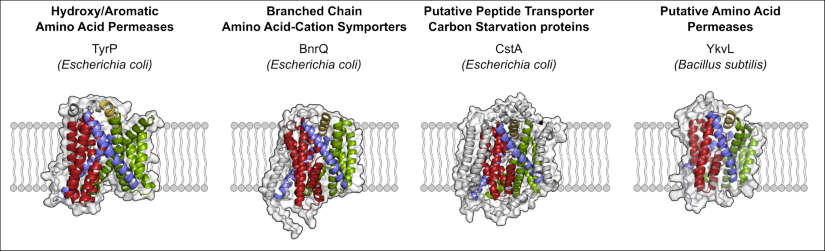
\includegraphics[width=5.5in]{Figures/leutintro_unknowns.pdf}
 \caption[Predicted structural models of proteins belonging to LeuT-fold families with no representatives in the PDB.]{Predicted structural models of proteins belonging to LeuT-fold families with no representatives in the PDB. Transporter families are defined by the Transporter Classification Database, and each model was generated using AlphaFold2.}
\label{fig:leutintro_unknowns}
\end{figure}

\subsection{Functional variation within the LeuT fold}

Retention of this ten-helix core is all the more remarkable considering the extent to which the functions, ligands, and sequences of these proteins differ. Although the majority of LeuT-fold proteins studied thus far cotransport their substrates and driving ions, others exchange them in opposite directions (symport and antiport, respectively \citep*{Forrest2009}). The centrally located substrate-binding site, shared by symporters and antiporters, accommodates ligands ranging in size and charge from halogen ions and divalent metals to sugars and aromatic amino acids. Its manipulation by mutagenesis has been shown to alter substrate specificity profiles in LeuT (\gls{nss}) \citep*{Piscitelli2011, Zomot2007}, GAT-1 (\gls{nss}) \citep*{Zomot2007}, and BetP (\gls{bcct}) \citep*{Perez2014}, highlighting the involvement of this region in identifying and trafficking ligands.

Beyond plasticity at this specific site, structural features decorating the core transporter further contribute to functional specialization. A remarkable example is SLC38A9, which both exports amino acids from the lysosome and activates the regulatory complex mTORC1 under nutrient-rich conditions \citep*{Rebsamen2015, Wang2015}. An N-terminal domain elegantly couples these two functions by binding to the cytoplasmic cavity \citep*{Lei2021} and, following displacement by the transported substrate arginine, releases and binds to GTPases involved in downstream signaling \citep*{Fromm2020}. In an interesting case of convergent evolution, the C-terminal domain of the pH-dependent \gls{glu}/\gls{gaba} exchanger GadC arrests transport by binding to the intracellular cavity at neutral pH in a nearly identical conformation \citep*{Ma2012}. Autoinhibition by disordered terminal domains has also been directly visualized in several potassium-chloride symporters \citep*{Chi2021, Xie2020}. In other proteins, such as eukaryotic \gls{nss}s, disordered termini instead regulate transport by interacting with a range of cytoplasmic proteins \citep*{Cooper2019, Karam2018}. In BetP, a cytoplasmic C-terminal helical domain regulates transport in response to osmotic stress \citep*{Gueler2016, Kraemer2009}. These domains often go unobserved in structural studies \citep*{Coleman2016, Liu2019, Penmatsa2013} due to truncation or intrinsic disorder, prompting speculation regarding their role in transport.

\newpage

\subsection{Quaternary structures adopted by LeuT-fold transporters}

Recent structures obtained by \gls{cryoem} have bolstered the diversity of quaternary structures known to be adopted by these proteins. Whereas X-ray crystallography demonstrated that LeuT-fold transporters can assemble as homodimers (AdiC, vSGLT) \citep*{Faham2008, Gao2009}, homotrimers (BetP, CaiT) \citep*{Ressl2009, Schulze2010}, or heterodimers (GkApcT) \citep*{Jungnickel2018}, due to technical limitations only compact binding interfaces were observed. By contrast, oligomers visualized by \gls{cryoem} reveal a multitude of weaker, more flexible, and in some cases asymmetric binding interfaces \citep*{Chew2019, Lee2019, Oda2020, Tascon2020, Yan2020a, Yan2020b, Yan2019, Yan2020}. For example, the eukaryotic \gls{apc} transporters Lat1, Lat2, and xCT each associate with 4f2hc (also called CD98hc) \citep*{Jeckelmann2020, Oda2020, Yan2019, Yan2020}, a protein with a large extracellular domain and a single transmembrane helix that is uninvolved in transport (Figure \ref{fig:leutintro_panel}). The homologous \gls{apc} transporter $\mathrm{b^{(0,+)}AT1}$ further assembles into a dimer of dimers with rBAT, each of which resemble the Lat/4f2hc complexes \citep*{Wu2020, Yan2020a}. This dimer-of-dimers arrangement was even observed in the \gls{nss} $\mathrm{b^{0}AT1}$, which associates with Angiotensin-converting enzyme 2 (the experimental structure of this tetramer was determined as part of a larger complex involving the SARS-CoV-2 spike protein) \citep*{Yan2020b}. Notably, the N-terminal transmembrane helices of rBAT and 4f2hc bind to the hash domains of $\mathrm{b^{(0,+)}AT1}$ and the Lats, respectively, at a similar position as the C-terminal transmembrane helix of ACE2 to $\mathrm{b^{0}AT1}$. Separately, the eukaryotic \gls{ccc}s \citep*{ Chew2019, Chi2020, Liu2019, Reid2020, Yang2020} and the bacterial potassium transporter KimA \citep*{Tascon2020} both fold as homodimers with large domain-swapped cytoplasmic regions. Divergence in both the sequences of these protein families and the structures of their cytoplasmic domains may highlight a recurrent quaternary assembly mechanism, the extent of which has not yet come to light.

Finally, in many cases, the oligomeric interfaces observed by \gls{cryoem} appear to be weaker and more flexible than suggested by the crystal structures. In both Lat1 and KCC1, for example, substantial interdomain movements have been reported when comparing their respective inward-facing apo and outward-facing inhibitor-bound states \citep*{Liu2019, Yan2021, Yan2019, Yan2020, Zhao2020}. Molecular dynamics simulations of the homodimer KimA suggested that contacts between the two transport domains are transient and fleeting, as these domains are tethered to one another only by their intertwined cytoplasmic domains \citep*{Tascon2020}; similar observations were experimentally made in \gls{ccc}s \citep*{Chi2021}. Such arrangements sharply contrast with the interfaces observed in vSGLT \citep*{Faham2008, Watanabe2010}, BetP \citep*{Ressl2009}, and other oligomers determined by crystallography, and hint at future discoveries regarding how these transporters interact as part of larger complexes.

\subsection{Recurring elements of substrate binding}\label{sec:ligands}

These unique structural features and arrangements surround a highly conserved ten-helix architecture shown in Figure \ref{fig:leutintro_arch}.C that, in several cases, have been shown to retain ligand-binding modes across distantly related proteins (Figure \ref{fig:leutintro_ligands}). A widely discussed example is the conserved sodium site, termed Na2, found in the majority of sodium-coupled symporters \citep*{Faham2008, Ressl2009, Wahlgren2018, Weyand2008, Yamashita2005}. In fact, the Na2 site's recurrence in this fold prompted Chew \emph{et al.} to assign its position to the sodium-binding site in the sodium/potassium/chloride symporter NKCC1, which was subsequently corroborated by molecular dynamics simulations and mutagenesis experiments that severely abrogated transport \citep*{Chew2019, Janos2021}. Among symporters that bind two sodium ions (\gls{nss}s, SiaT \citep*{Wahlgren2018}, BetP \citep*{Khafizov2012}), no such conservation is observed in the position of the other sodium ion. In proton-coupled symporters and amino acid exchangers, positively-charged residues occupy this position (lysine in ApcT, GkApcT, and BasC, and arginine in CaiT \citep*{Errasti-Murugarren2019, Gao2009, Jungnickel2018, Schulze2010, Tang2010}), highlighting the malleability of substrate coupling throughout the fold. A noteworthy exception is the sodium-coupled amino acid symporter AgcS, which coordinates its only sodium at a position equivalent to LeuT's Na1 site, leaving the Na2 site unoccupied \citep*{Ma2018}. This is despite its alanine binding site overlapping nearly perfectly with the substrate binding sites of unrelated amino acid transporters from the \gls{nss} and \gls{apc} families (Figure \ref{fig:leutintro_ligands}.C). To our knowledge, no cations besides sodium ions and protons have been observed in this site, and no comparable degree of structural conservation has observed at other ligand-binding sites, such as those involved in binding potassium (transported by \gls{sert}, as well as the \gls{kup} and \gls{ccc} families) or chloride (transported by \gls{nss}s and \gls{ccc}s).


\begin{figure}[h]
\centering
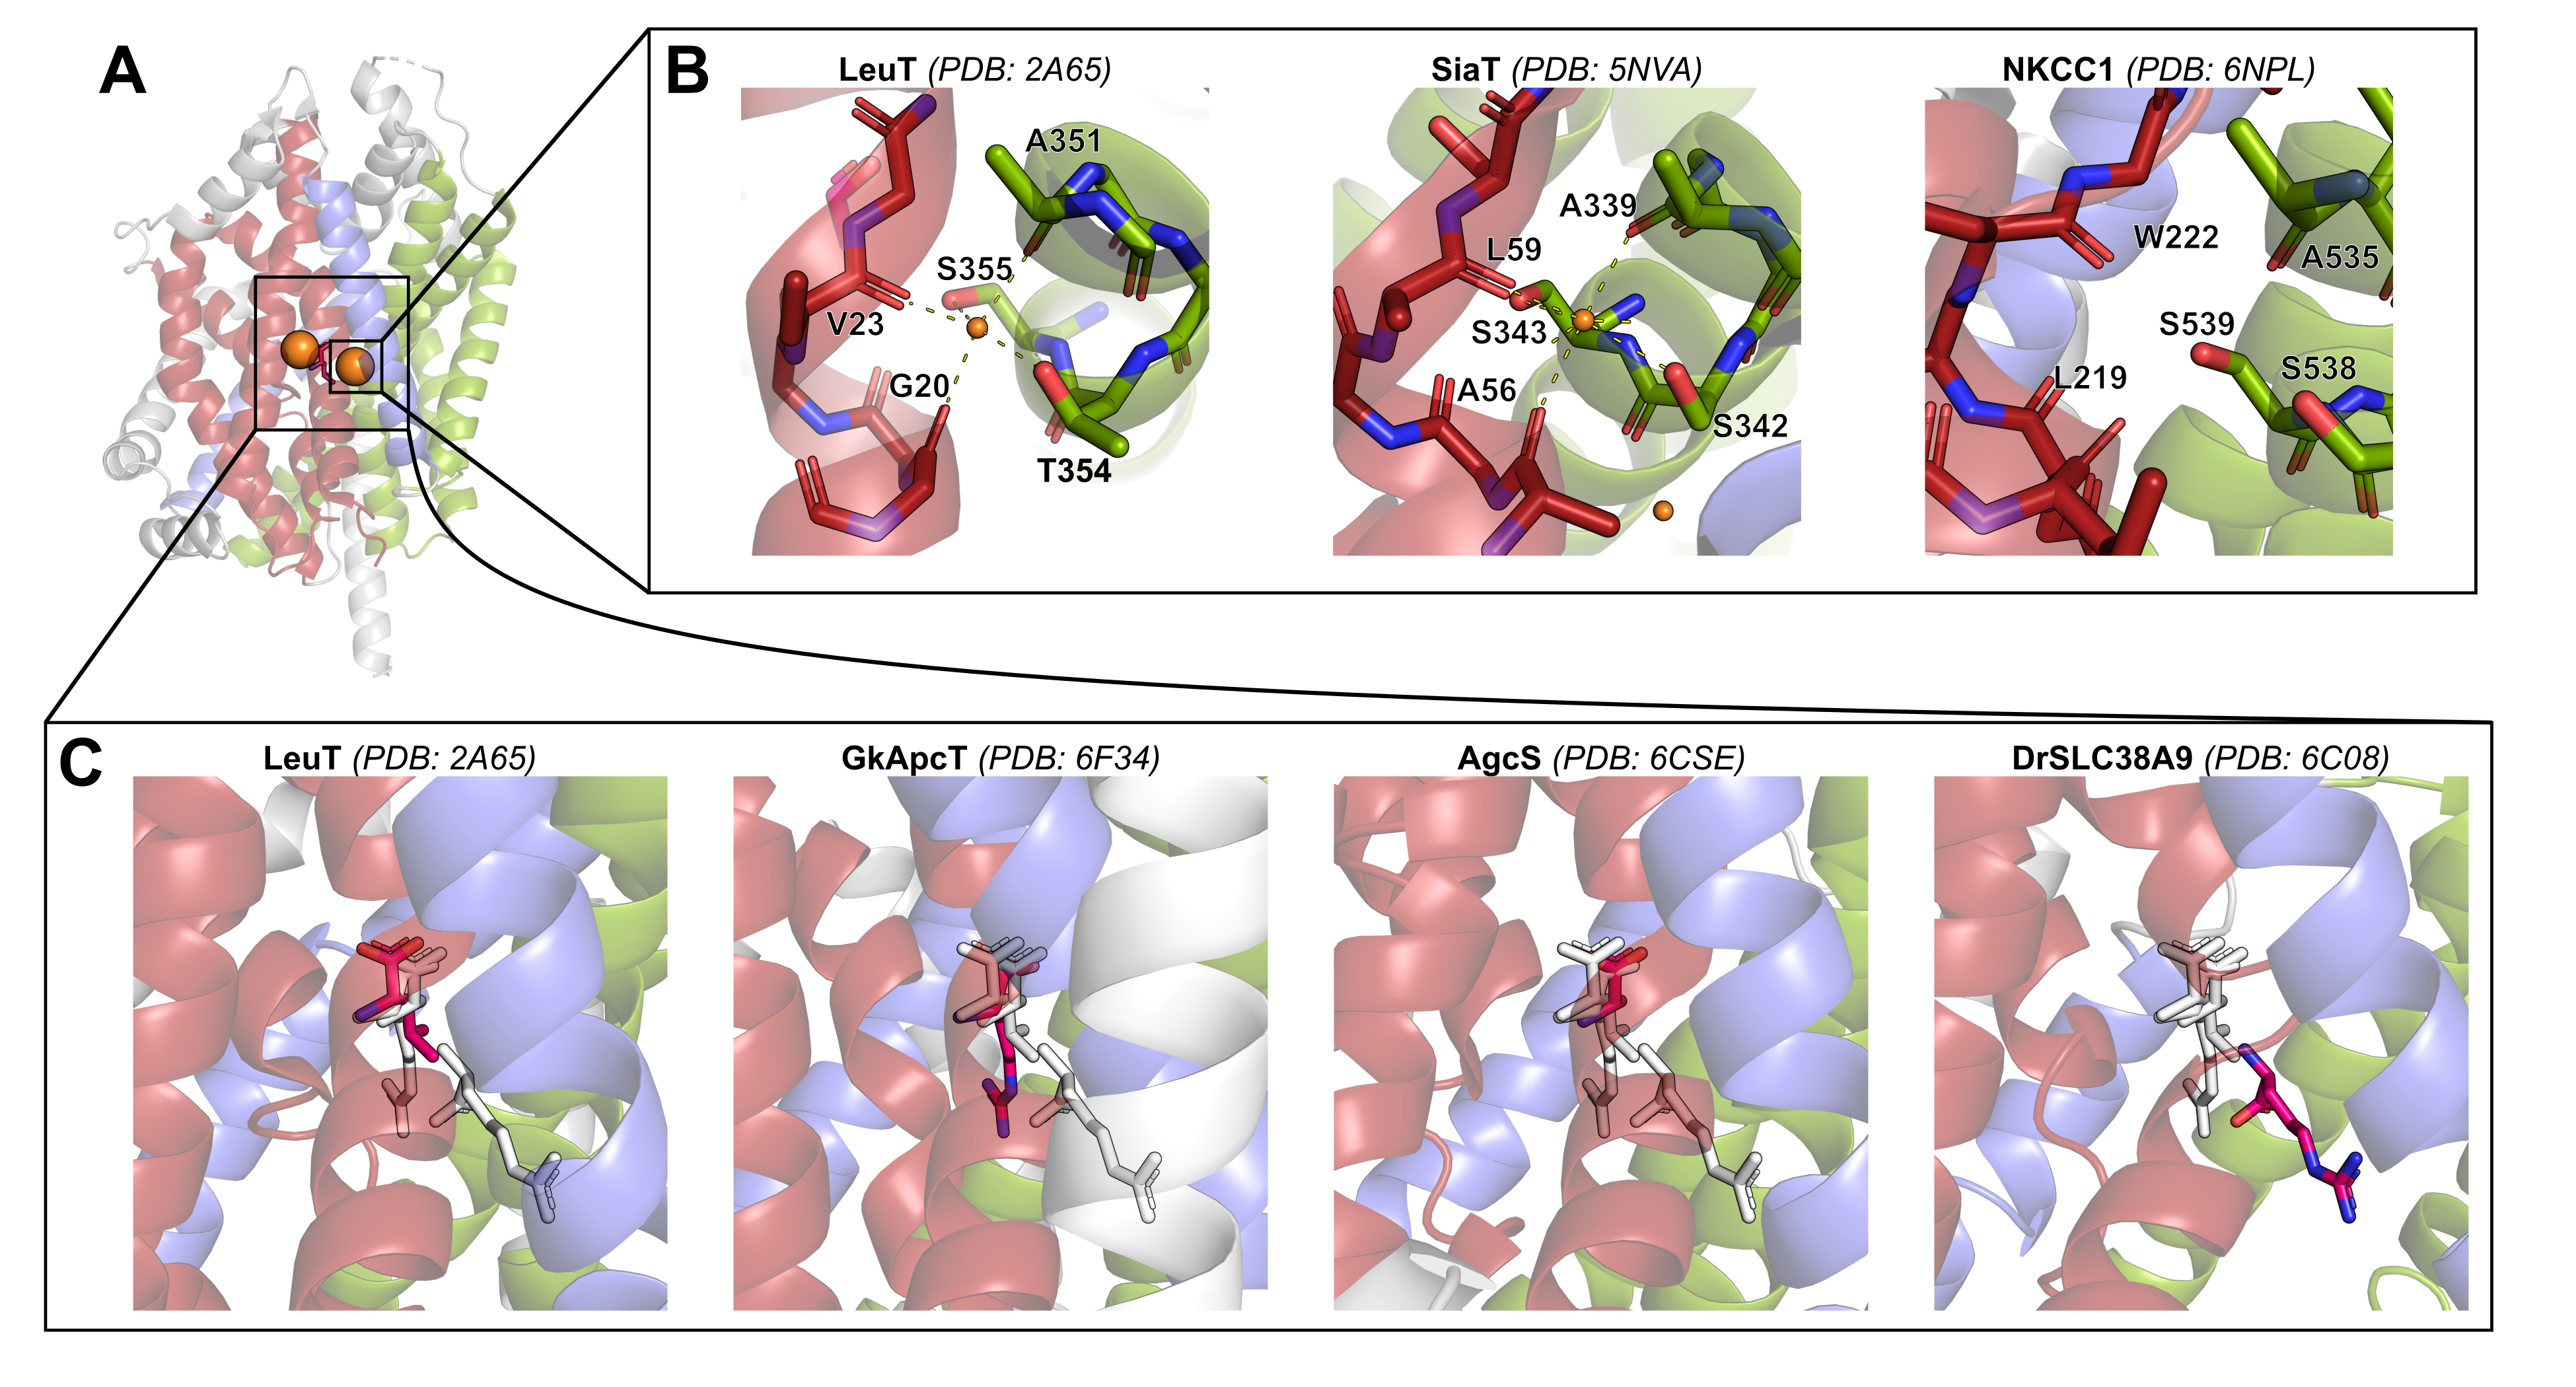
\includegraphics[width=6.5in]{Figures/leutintro_ligands_hoz.pdf}
 \caption[Examples of conserved ligand coordination.]{Examples of conserved ligand coordination. (A) Sodium ions (orange) and leucine (pink) in LeuT. (B) Conservation of the Na2 site. (C) Partial recurrence of amino acid binding modes. Substrates colored white are shared in all four panels.}
\label{fig:leutintro_ligands}
\end{figure}


\section{Alternating access inferred from crystal and cryo-EM structures}

At the molecular level, alternating access involves the opening and closing of gates providing passage to the substrate-binding site from either the intracellular or extracellular spaces \citep*{Jardetzky1966} For transporters with the LeuT-fold, this principally manifests as isomerization between \gls{of} and \gls{if} states using a "rocking bundle" mechanism that forbids substrate entry and exit from the cytoplasmic or periplasmic side of the membrane, respectively \citep*{Forrest2009}. Despite their co-classification, however, closer examination at structural changes in these proteins reveals a striking lack of consensus over the molecular details of alternating access. Conformational divergence as the rule, not the exception, became apparent nearly a decade ago with the publication of high-resolution structures of Mhp1 \citep*{Shimamura2010, Weyand2008}, BetP \citep*{Ressl2009}, and LeuT \citep*{Kazmier2017, Krishnamurthy2012, Yamashita2005}, and has since been reinforced by similar studies in SERT \citep*{Coleman2016, Coleman2019}, DraNramp \citep*{Bozzi2016, Bozzi2019}, and Lat1/4f2hc (Figure \ref{fig:leutintro_aa}) \citep*{Yan2021, Lee2019, Yan2021}. Additional structures of AdiC \citep*{Fang2009, Gao2009} and vSGLT \citep*{Faham2008, Watanabe2010} in both open and occluded conformations, though limited to \gls{of} and \gls{if} states, respectively, further expand the ways in which these transporters grant access to the substrate-binding site. Overall, comparison of pairs of structures reveals fundamental differences in which helices move and which stay fixed (Figure \ref{fig:leutintro_rmsf}).

\begin{figure}[h!]
\centering
\includegraphics[width=6.5in]{Figures/leutintro_aa.pdf}
 \caption[Variations in structural dynamics within the LeuT-fold.]{Variations in structural dynamics within the LeuT-fold. Conformational dynamics of LeuT-fold transporters show striking differences in how alternating access is carried out. Dynamic and static helices are depicted as ribbons and cylinders, respectively. Bottom left: No individual \gls{sss} has been characterized in both \gls{of} and \gls{if} conformations.}
\label{fig:leutintro_aa}
\end{figure}

\begin{figure}[h!]
\centering
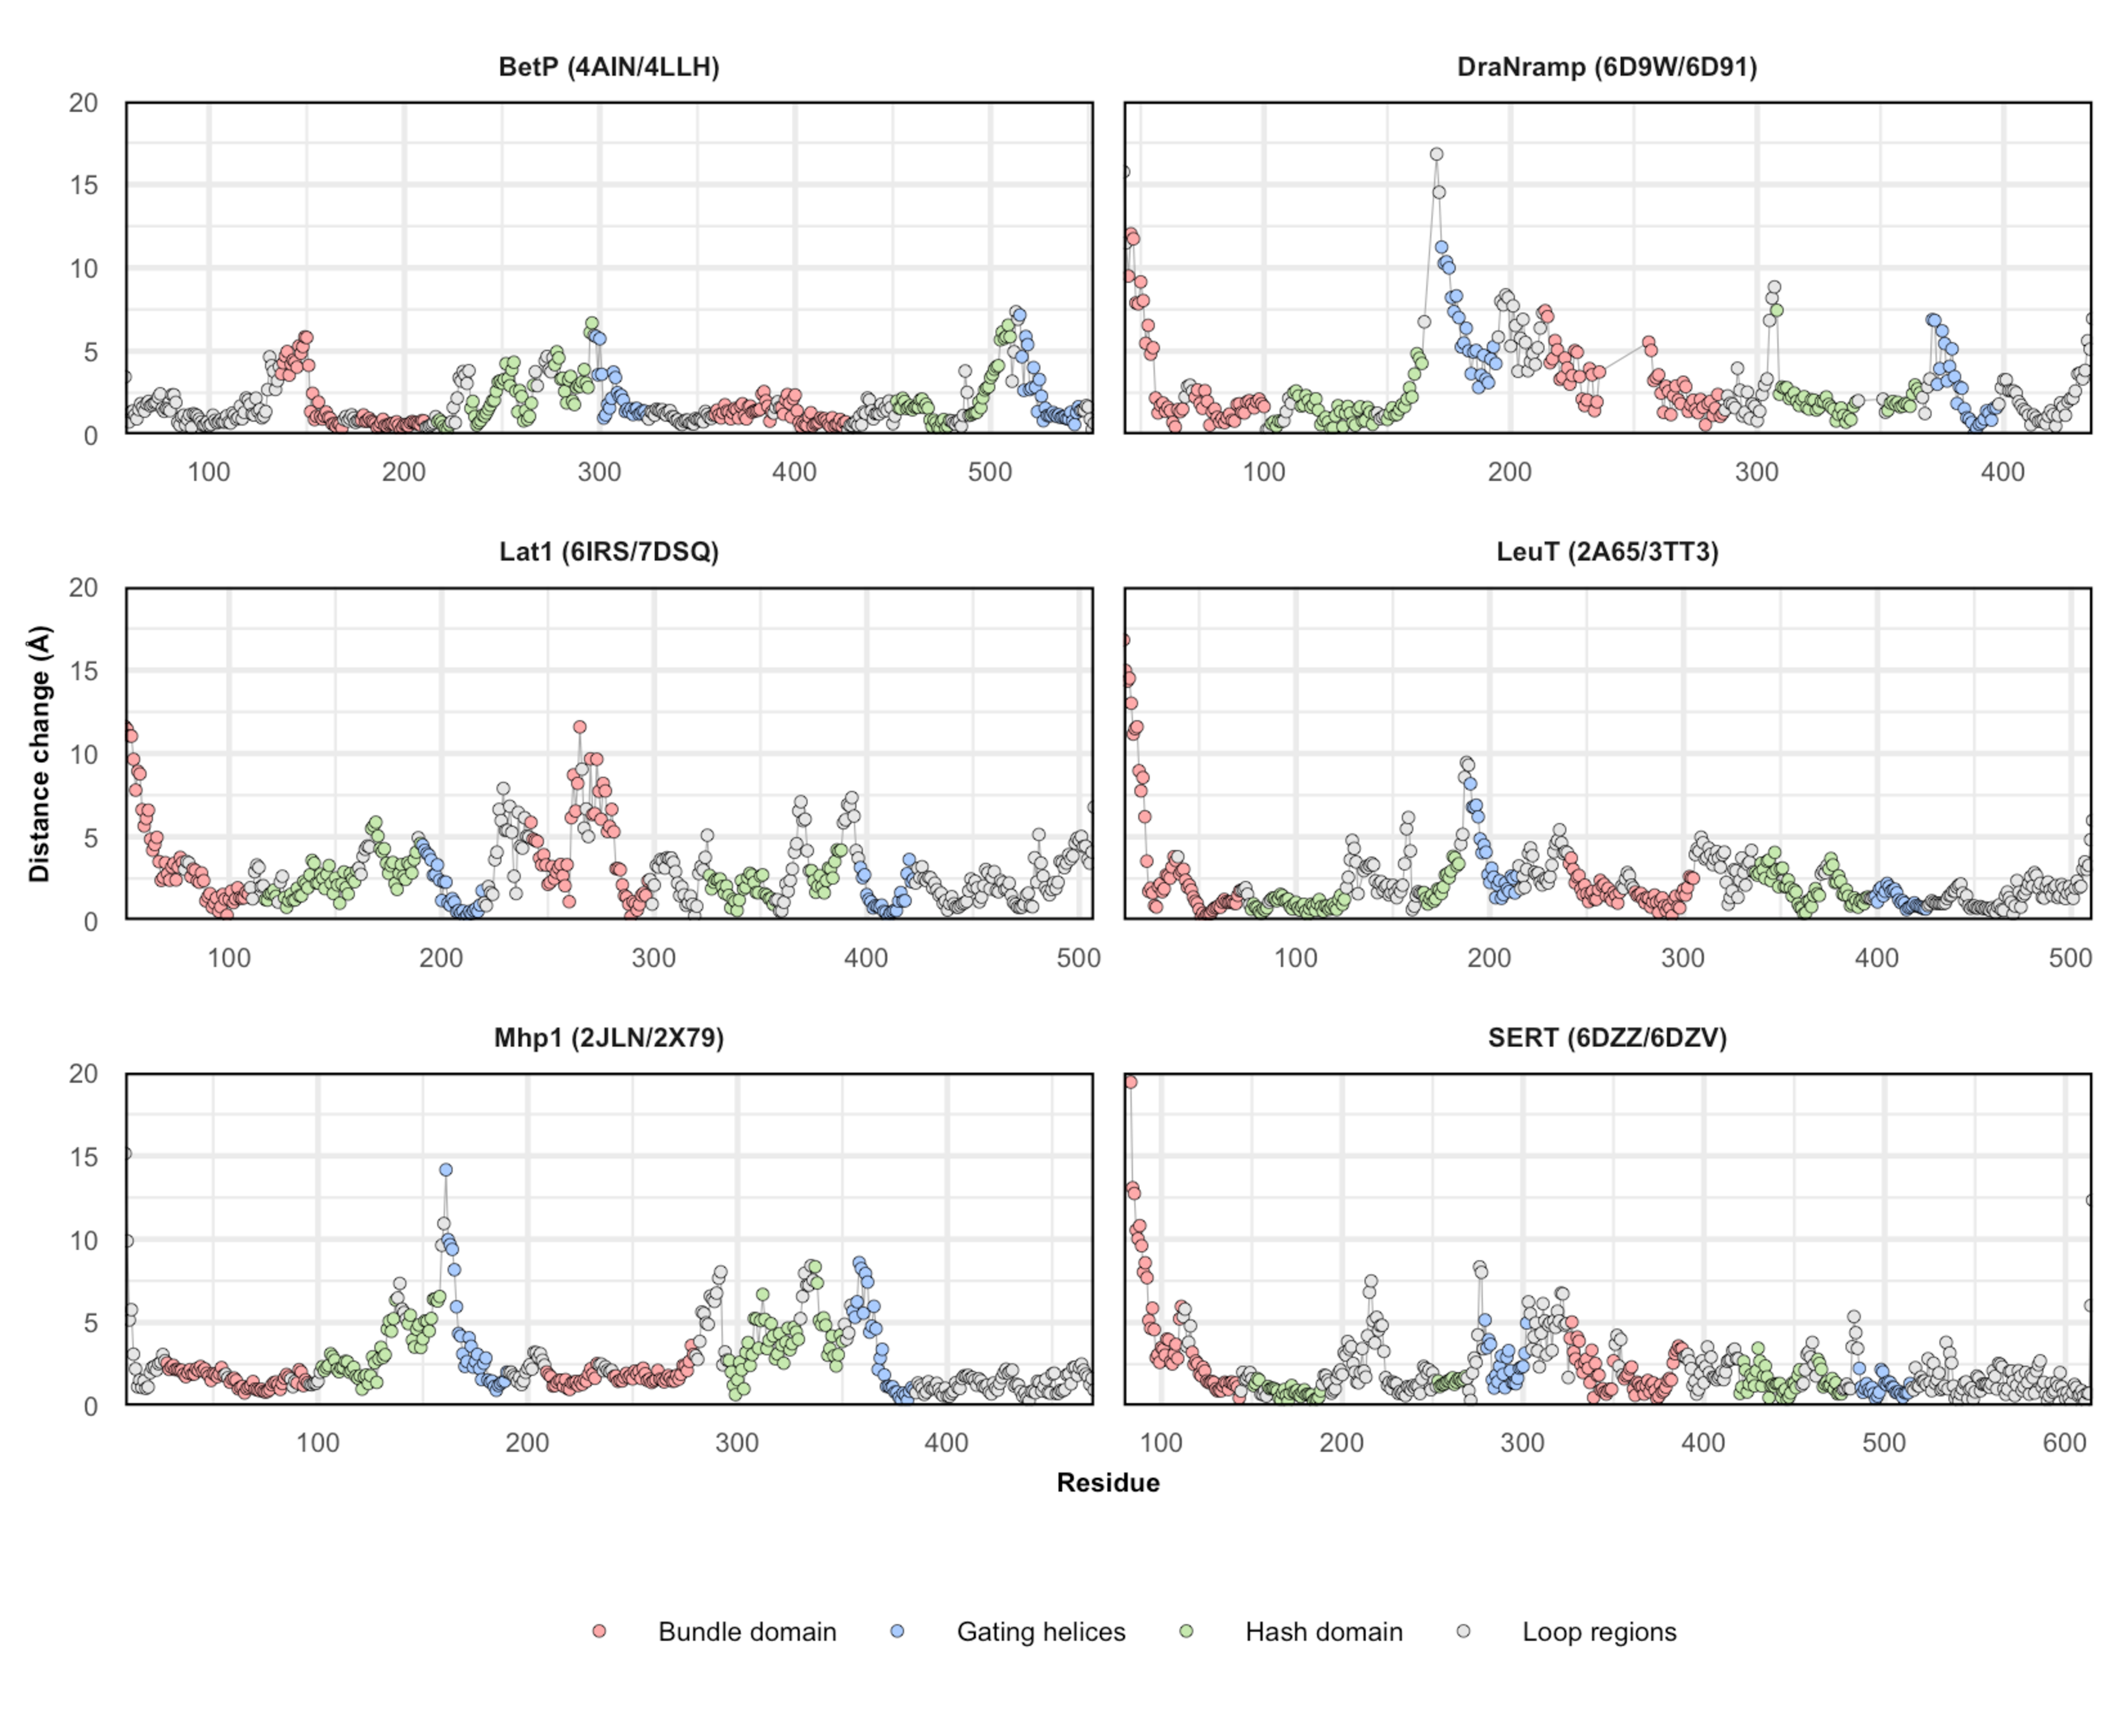
\includegraphics[width=6.5in]{Figures/leutintro_rmsf.pdf}
 \caption[Residue-level movements during IF-to-OF isomerization in various LeuT-fold proteins.]{Residue-level movements during \gls{if}-to-\gls{of} isomerization in various LeuT-fold proteins. Unresolved residues omitted from the plot. All structures were aligned using TM-Align \citep*{Xu2010, Zhang2005}.}
\label{fig:leutintro_rmsf}
\end{figure}

\subsection{Movement of gating helix TMH5}\label{sec:leutintro_tm5}

Along with the intracellular loop preceding it, \gls{tmh}5 ranks among the most consistently mobile and dynamic regions in the transporters studied so far \citep*{Stolzenberg2017}.  In \gls{of} conformations, \gls{tmh}5 nestles against the bundle domain helices \gls{tmh}1a and \gls{tmh}6b, forming the highly ordered intracellular "thick gate". In the IF state, by contrast, opening of the intracellular vestibule is driven by rearrangements that vary across families and even individual proteins within families. The contribution of \gls{tmh}5 to alternating access has been most extensively studied in \gls{nss}s \citep*{Stolzenberg2017}. A $\mathrm{G_{X}NP}$ sequence, strictly conserved within the family and partially conserved throughout the fold, putatively mediates both bending and unfolding motions instrumental to the initiation of substrate release (Figure \ref{fig:leutintro_tm5tm10}). Mutagenesis of glycine or proline severely abrogates transport \citep*{Malinauskaite2014}, highlighting the importance of the dynamic processes facilitated by this motif. First observed in a substrate-bound \gls{if}-occluded conformation of MhsT \citep*{Malinauskaite2014}, partial unwinding of \gls{tmh}5 has been corroborated in several \gls{nss}s by \gls{hdxms} studies under conditions promoting the \gls{if} conformation of each protein \citep*{Adhikary2017, Merkle2018, Moeller2019, Nielsen2019}. However, although \gls{if}-open structures of LeuT and \gls{sert} show this helix protruding out from the rest of the transporter \citep*{Coleman2016, Gotfryd2020, Krishnamurthy2012}, orthogonal measurements in LeuT both suggest that under \gls{if}-promoting conditions it adopts conformations where the intracellular cavity is occluded, rather than open \citep*{Kazmier2014, Shi2008, Zhao2011, Zhao2010}. As is elaborated below in Section \ref{sec:leutintro_nss_dynamics} below, however, these results are qualified by the frequent use of leucine, which has a low transport rate and nanomolar binding affinity \citep*{Singh2008}. Subsequent solution-state experiments bound to different amino acids found that quenching of fluorescent probes attached to the intracellular half of \gls{tmh}5 inversely correlated with transport rate \citep*{Billesbølle2015}, suggesting that this \gls{if}-occluded conformation may be less stable, relative to \gls{if}-open, when transporting substrates with higher turnover rates such as alanine. Nevertheless, in conjunction with other findings discussed below in Section \ref{sec:leutintro_nss_dynamics}, this points to a mechanism in which \gls{tmh}5 preferentially adopts the partially unwound occluded conformation when bound to its substrate but transiently bends to release substrates.

It is notable that \gls{tmh}5 adopts a similar, but not identical, conformation in \gls{if}-open Mhp1, which shares this $\mathrm{G_{X}NP}$ sequence \citep*{Shimamura2010}. Despite this agreement, \gls{epr} measurements revealed a degree of disorder in \gls{tmh}5 altogether absent from similar measurements carried out on LeuT in the presence of leucine \citep*{Kazmier2014a}. Interestingly, ApcT also shares a LeuT-like bend despite lacking a proline in \gls{tmh}5 at the equivalent position \citep*{Shaffer2009}. Since its structure has only been determined in a single conformation, and since its homologs such as GadC and BasC maintain a straight conformation of this helix \citep*{Jungnickel2018, Ma2012}, the extent to which the aforementioned \gls{nss} movements occur in ApcT and its homologs is unclear \citep*{Shi2010}. Finally, although \gls{tmh}5 is also involved in opening the intracellular cavity in DraNramp \citep*{Bozzi2019}, which also lacks the conserved mid-helical proline, it undergoes a rigid-body up-and-out translation rather than bending and unfolding. Many other \gls{if} structures, such as those observed in vSGLT and GkApcT, lack a fully resolved stretch of residues corresponding to \gls{il} 2, located between \gls{tmh}s 4 and 5, indicating a high degree of heterogeneity in the crystal lattice or \gls{cryoem} grid \citep*{Jungnickel2018, Watanabe2010}. Ultimately, the conformational variation observed across the fold in this loop and helix, combined with solution-state data indicative of local disorder, suggests that the protruded conformation observed in some proteins, though perhaps physiologically relevant and likely fundamental to the transport cycle, may not represent a well-defined low-energy state.

\begin{figure}[h]
\centering
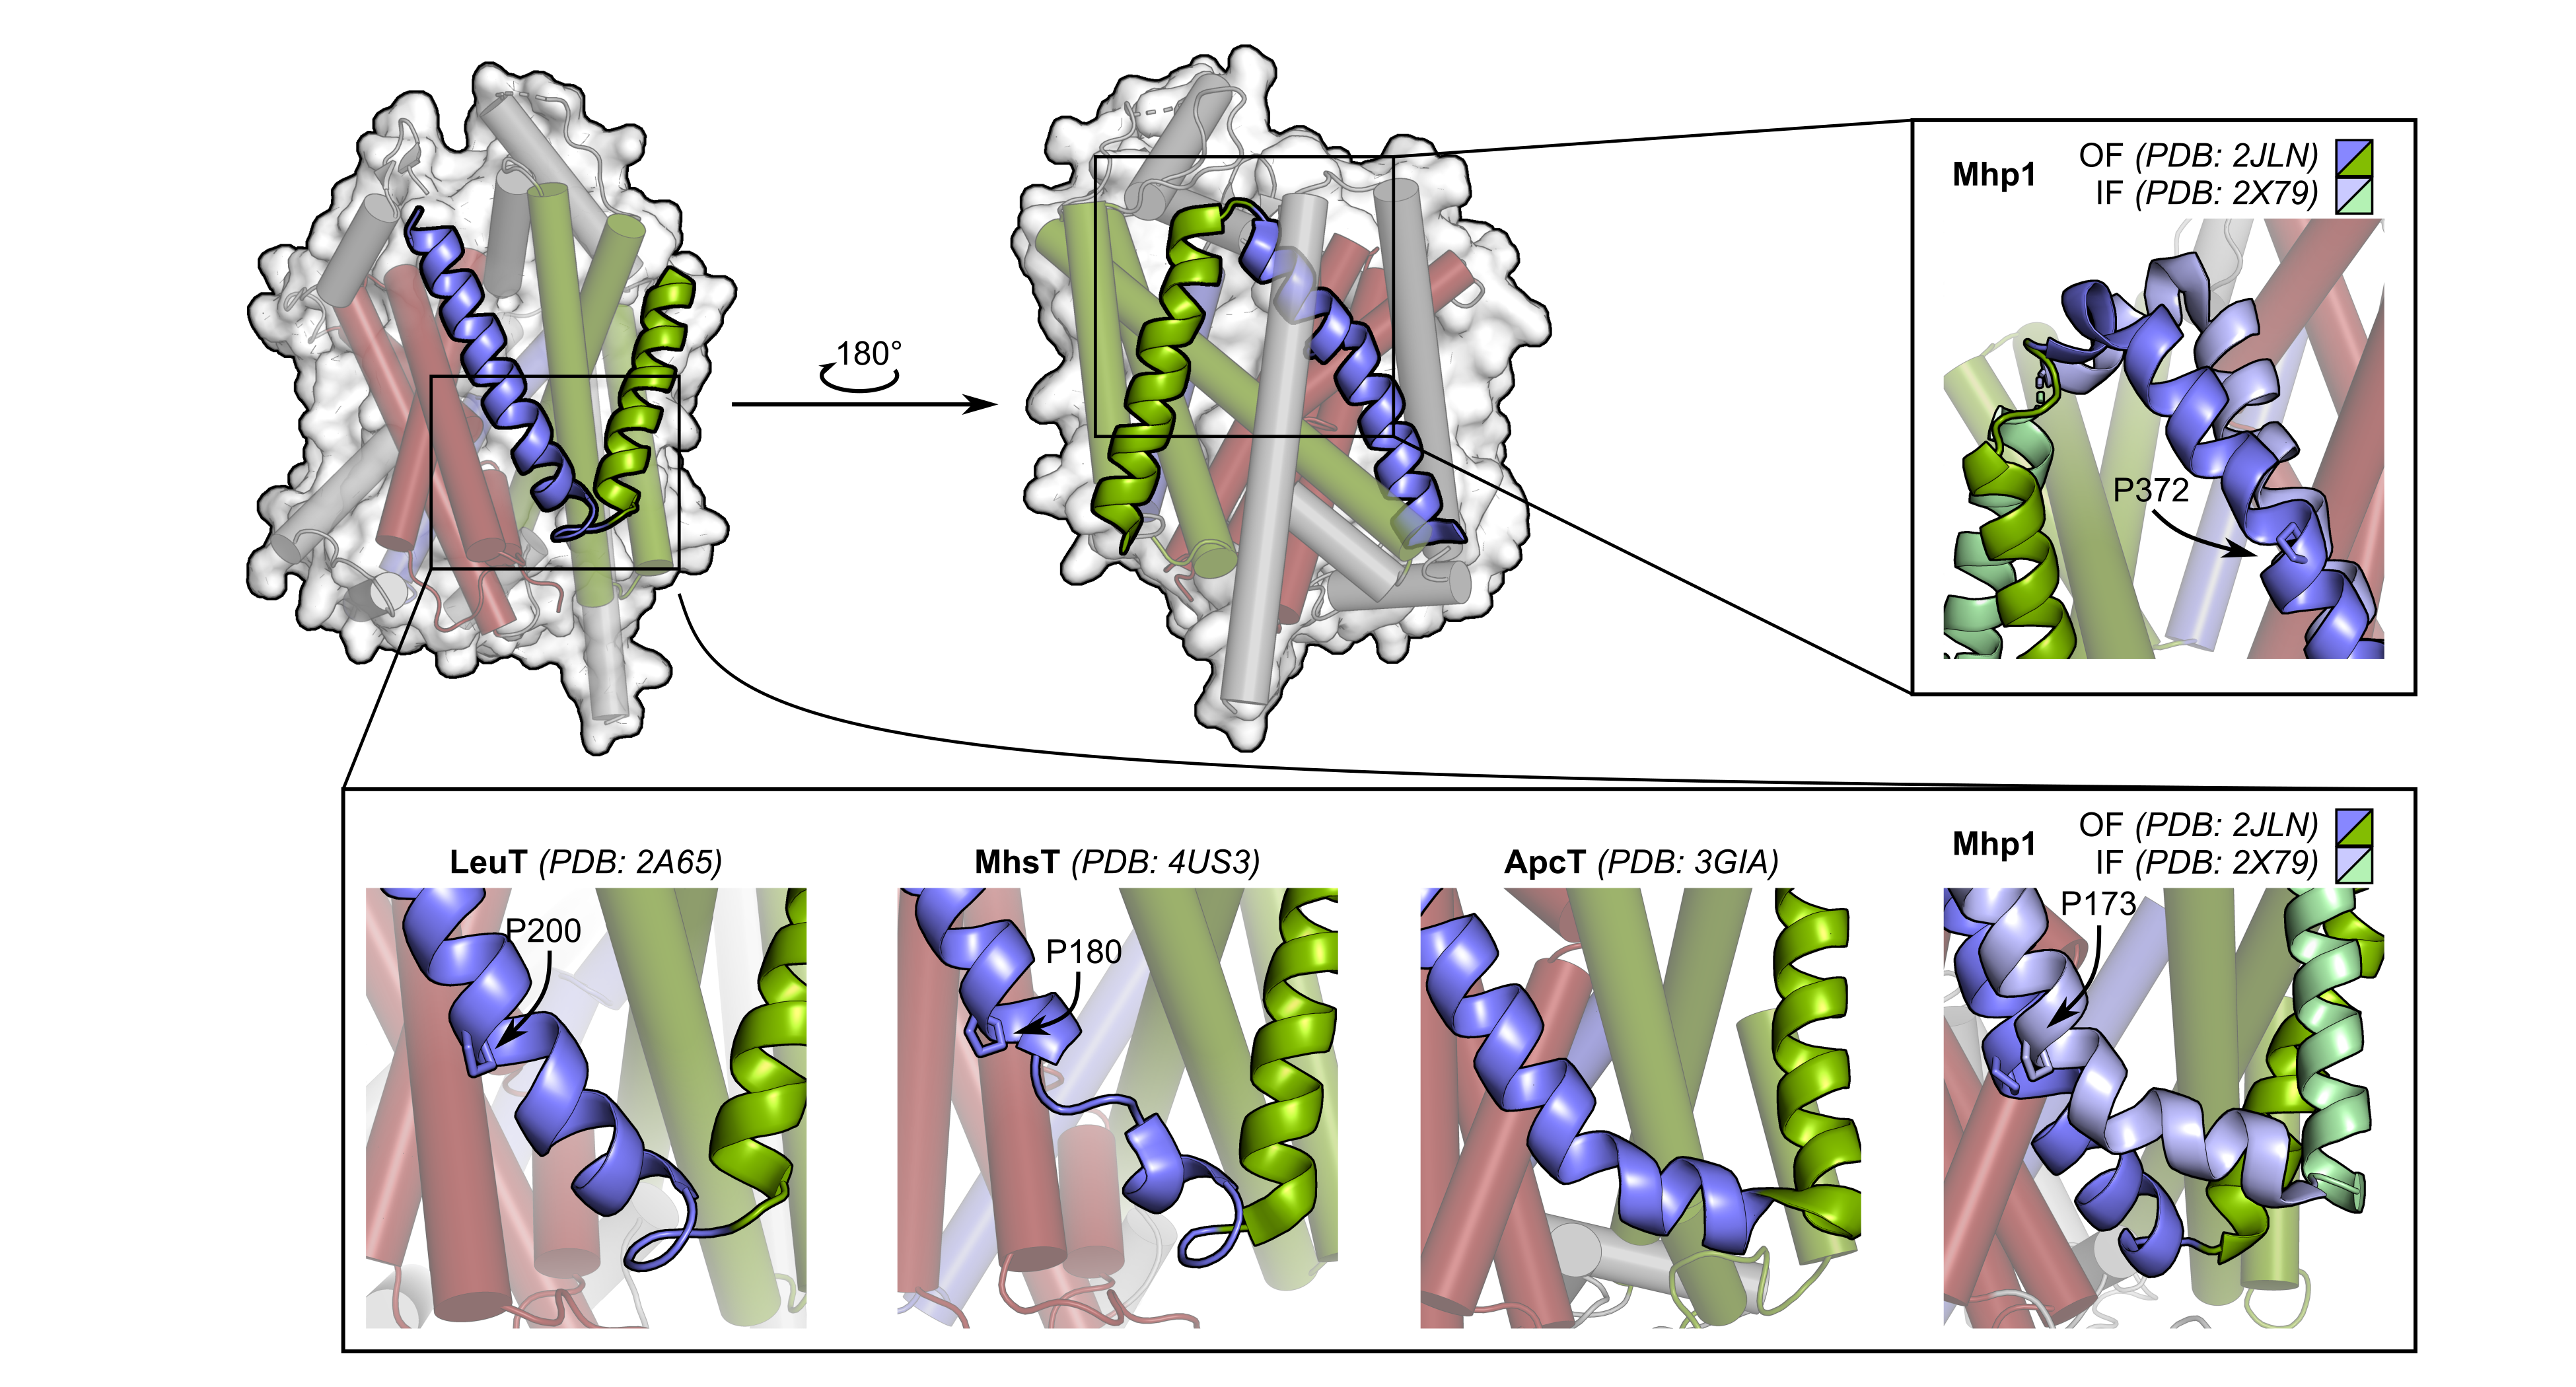
\includegraphics[width=6.5in]{Figures/leutintro_tm5tm10_hoz.pdf}
 \caption[Pivoting of TMH5 and TMH10 is observed in a subset of LeuT-fold transporters.]{Pivoting of \gls{tmh}5 and \gls{tmh}10 is observed in a subset of LeuT-fold transporters. Top left: LeuT with \gls{tmh}4/5 and TM9/10 highlighted. Bottom: Movements of \gls{tmh}5 observed in \gls{nss}s, ApcT, and DraNramp in the IF state. Conserved proline residues are highlighted in LeuT, MhsT and Mhp1. Top right: Movement of \gls{tmh}0 in Mhp1.}
\label{fig:leutintro_tm5tm10}
\end{figure}

\subsection{Movement in gating helix TMH10}

Movement in \gls{tmh}10, despite its pseudosymmetry to \gls{tmh}5, is less frequently observed (Figure \ref{fig:leutintro_tm5tm10}.B). In \gls{nss}s, for example, no evidence has been collected that show involvement in either ligand-dependent conformational dynamics, or partial unwinding \citep*{Kazmier2014a, Merkle2018, Moeller2019, Nielsen2019}. Mhp1 shows some partial symmetry of \gls{tmh}10 to \gls{tmh}5 in both sequence and structure, with comparable increases in conformational heterogeneity detected by \gls{epr} under \gls{of}-stabilizing experimental conditions (Figure \ref{fig:leutintro_tm5tm10}) \citep*{Kazmier2014, Shimamura2010, Weyand2008}. However, the movement inferred from crystal structures is less dramatic than that of \gls{tmh}5. In both BetP and DraNramp, differences between their \gls{of}-closed and open conformations in this region, though less drastic than in Mhp1, are nonetheless unmistakable; indeed, the corresponding proline in \gls{tmh}10 facilitating this bend is strictly conserved in the \gls{bcct} family and partially conserved among \gls{nramp}s \citep*{Bozzi2021, Schulze2010}. Although the \gls{apc} transporter AdiC both shares this specific residue and shows evidence of this structural movement, its structural similarity to the eukaryotic homolog Lat1, which instead has a cysteine at the equivalent position, indicates that placement of the proline halfway across \gls{tmh}10 may be coincidental \citep*{Fang2009, Yan2021}.

\subsection{Helical pivoting in the bundle domain}\label{sec:leutintro_bundle}

LeuT's twofold pseudosymmetry initially appeared to imply that a rigid-body rotation of the bundle domain relative to the rest of the structure mediates alternating access \citep*{Forrest2008}. This proposal, although elegant, failed to predict subsequent structural evidence in two key respects. First, the contribution of this domain to alternating access, although prominent in some proteins, is far from universal. Movement in ancillary helices and loop regions has been observed in every protein studied thus far. Second, the bundle domain virtually never moves as a rigid body. The exception, Mhp1, locks the bundle domain into place and instead pivots the hash domain and gating helices around this scaffold \citep*{Weyand2008} (see Section \ref{sec:leutintro_hash} below).

Movements in \gls{tmh}1a embody the variable intradomain dynamics observed in these helices. Its apparent dissociation from the rest of the intracellular vestibule, observed in X-ray and \gls{cryoem} structures of \gls{nss}s and \gls{nramp}s \citep*{Bozzi2019, Coleman2019, Ehrnstorfer2014, Krishnamurthy2012}, has been verified in solution (both families, it should be noted, lack N-terminal helices and oligomeric interfaces capable of restricting the dynamics of \gls{tmh}1a; see Figure \ref{fig:leutintro_rmsf}). Particular controversy surrounds the relevance of the signature 45° pivot observed in LeuT, which has been attributed to both the use of short-chain detergents commonly used in membrane protein crystallography \citep*{Moeller2020, Sohail2016}, as well as alanine mutagenesis of a conserved tyrosine residue essential for function \citep*{Krishnamurthy2012, Loland2002}. Molecular dynamics simulations of LeuT's \gls{if}-open crystal structure in a lipid bilayer later revealed the steep energetic cost of this movement into a more physiological membrane environment \citep*{Sohail2016}. Although this brought attention to the contribution of the membrane mimetic (along with a high-affinity antibody) in stabilizing such an extreme conformer, these findings, alongside experimental measurements obtained using both \gls{lret} \citep*{Sohail2016} and \gls{hdxms} \citep*{Adhikary2017} in lipid environments, nonetheless corroborated the more general hypothesis that \gls{tmh}1a becomes conformationally disordered in the \gls{if}-open state. Nevertheless, as these experiments were executed on similar tyrosine-to-alanine mutants, they do not address the extent to which this \gls{if}-open conformation is sampled by the wildtype protein in solution. For example, \gls{epr} measurements on equivalent tyrosine-to-alanine mutants recorded a comparable degree of disorder in \gls{tmh}1a; by contrast, no such dynamics were observed in variants without this mutation \citep*{Kazmier2014a, Merkle2018}. Follow-up experiments in \gls{sert} would paint a similar picture, with ibogaine, a ligand used to stabilize the \gls{if}-open structure during \gls{cryoem} studies, taking the role of this tyrosine-to-alanine mutation in LeuT \citep*{Coleman2019, Moeller2019}. Overall, the data suggest that the \gls{if}-open conformations of \gls{nss}s, and perhaps other proteins with similar conformational dynamics, transiently sample disordered \gls{tmh}1a states as part of their function, dovetailing with the conclusions on \gls{tmh}5 discussed above.

A similar pattern of increased disorder under \gls{if}-open-promoting conditions has also been observed in the intracellular side of \gls{tmh}7. In addition to the movements observed crystallographically, \gls{tmh}7 in LeuT appears to partially unfold under \gls{if}-favoring experimental conditions \citep*{Merkle2018}. For example, the eight N-terminal residues of this helix were not assigned to electron density in \gls{if}-open apo DraNramp \citep*{Bozzi2019}. The most pronounced motion of \gls{tmh}7 is likely found in Lat1, which swings over \SI{10}{\angstrom} to close its intracellular cavity \citep*{Yan2021}. As is discussed below, such a motion was suggested by, but not directly observed in, its bacterial homologs in the \gls{apc} family \citep*{Errasti-Murugarren2019, Ma2012}. Interestingly, no comparable movements are observed on the extracellular side of \gls{tmh}7. Unfortunately, the absence of data reporting the dynamics of transporters in the \gls{apc} family prevents any conclusions regarding increases in disorder in this helix from being established.

\gls{tmh}1b and \gls{tmh}6a, located on the extracellular sides of the protein, consistently undergo smaller scale but nonetheless significant dynamics essential to opening of the extracellular vestibule \citep*{Singh2008}. These helices appear to open the extracellular vestibule by moving in concert with the conserved helix \gls{el} 4, located between \gls{tmh}7 and \gls{tmh}8, in \gls{nss}s, \gls{apc} transporters, and \gls{nramp}s. While the observed movements of \gls{el}4 appear minor when compared to \gls{tmh}1a on the intracellular side, \gls{epr} spectroscopy data on LeuT indicate that crystal structures may understate the true extent to which these helices move \citep*{Kazmier2014}. Interestingly, on the intracellular side, no equivalent coupling between \gls{tmh}1a, \gls{tmh}6b, and \gls{il}1 has been detected to our knowledge. Indeed, unlike \gls{el}4, \gls{il}1 appears to be firmly stapled to the hash domain.

\subsection{The hash domain generally acts as a rigid body}\label{sec:leutintro_hash}

Relative to movements outlined above, independent helical movement within the hash domain are relatively rare. Mhp1 stands out in rocking this domain, alongside bending in \gls{tmh}5 and \gls{tmh}10, to fully mediate alternating access \citep*{Kazmier2014a, Shimamura2010, Weyand2008}. Similar movements were recorded in vSGLT using \gls{epr} \citep*{Paz2018}, although these coincided with additional movement distributed throughout the rest of the structure. As a point of contrast, other proteins limit their movements to bending of \gls{tmh}4 on the intracellular side and \gls{tmh}9 on the extracellular side to complement aforementioned movements of \gls{tmh}5 and \gls{tmh}10, respectively. The contribution of ancillary helices, which are frequently found adjacent to the hash domain, in explaining this phenomenon is unclear. In an interesting twist, a preprint publication describing the \gls{if}-to-\gls{of} transition in KCC1 proposes that alternating access is purely mediated by movement of \gls{tmh}3 and \gls{tmh}8, while \gls{tmh}4 and \gls{tmh}9 remain fixed \citep*{Liu2019, Zhao2020}.

\subsection{Conformational stabilization complicates the interpretation of these structures}

Importantly, many of these transporters, with Mhp1 and BetP being noteworthy exceptions, could only be coaxed into specific conformations using mutations, antibodies, or high-affinity transport inhibitors detrimental to function (see Tables \ref{tab:leutintro_proteins1} and \ref{tab:leutintro_proteins2}). In addition to the controversial use of a transport-abolishing tyrosine-to-alanine mutation in LeuT discussed above (Section \ref{sec:leutintro_bundle}) \citep*{Krishnamurthy2012}, stabilization of its \gls{if}-open state was also achieved by mutating a conserved tryptophan similarly found to be essential for function \citep*{Gotfryd2020}. Crystallographic capture of DraNramp in \gls{of} and \gls{if} conformations required glycine-to-arginine and glycine-to-tryptophan mutations near the unwound regions of \gls{tmh}1a and \gls{tmh}6a, respectively, that prevented isomerization by obstructing closure of the appropriate vestibule \citep*{Bozzi2016, Bozzi2019}. In human \gls{nramp}s, the equivalent missense mutation in \gls{tmh}1a is correlated with severely reduced iron uptake \emph{in vivo} \citep*{Barrios2012}, highlighting the extent to which transport function is impaired. Similarly, crystallization of \gls{if}-open vSGLT resulted from a lysine-to-alanine mutation that prevented ligand binding and showed no transport activity \citep*{Watanabe2010}. Capture of the OF-occluded conformation of AdiC, achieved using an aspartate-to-alanine mutation, may have played a role in stabilizing a ligand pose distinct from those observed in subsequent ligand-bound crystal structures of the wildtype protein \citep*{Gao2009}. Equivalent studies of the eukaryotic transporters \gls{sert} \citep*{Coleman2019}, Lat1 \citep*{Yan2021}, and KCC1 \citep*{Zhao2020} have employed a broad panel of potent inhibitors that preferentially bind to specific conformations. Whereas apo \gls{sert} readily crystallized in an \gls{of} conformation, capture of its \gls{if} conformation required the small molecule ibogaine \citep*{Coleman2019}. Similarly, both Lat1 and KCC1 were structurally characterized in \gls{if} conformations in the absence of ligands \citep*{Lee2019, Liu2019, Xie2020, Yan2020a} but could only be described in \gls{of} conformations using inhibitors \citep*{Yan2021, Zhao2020}. In each of these cases, the introduction of small molecules and/or inactivating mutations arrested transport by stabilizing conformers off-path with respect to the protein's functional cycle.

Nevertheless, assuming the physiological relevance of these structures, their comparison naturally prompts speculation regarding the evolutionary and/or functional basis for the variation in alternating access mechanisms. One proposal, made by the authors that determined the \gls{of} structure of KCC1, is the size of the ligand; only small-scale movements, limited to \gls{tmh}3 and \gls{tmh}8, are necessary for symport of the relatively small ions potassium and chloride \citep*{Zhao2020}. This hypothesis implies that larger substrates require larger movements and is supported by the observation that outward-locked DraNramp can transport protons, but not metals \citep*{Bozzi2019}. However, the small size of metals nonetheless raises questions about why DraNramp's \gls{of}-to-\gls{if} transition consists of such large-amplitude movements. Similarly, the relatively minor conformational changes observed in the transport cycle of BetP \citep*{Perez2012}, the substrates of which are comparable in size to amino acids, have been justified by function-specific adaptations. Ultimately, the insufficient data prevent any conclusions from being established in this respect.

\section{Connecting the dots: from structures to landscapes}

Proteins rarely navigate the conformational space accessible to them in the stepwise fashion suggested by depictions such as the one shown in Figure \ref{fig:leutintro_nss}. Mechanistic models of transport must necessarily, therefore, also map the conditions under which specific conformations occur. Secondary active transporters lack a molecular motor such as an ATPase and must therefore rely on the energy input provided by ions and ligands to undergo forward transport \citep*{Boudker2010}. The central question concerns how transporters harness this energy to undergo reconfigurations that ultimately result in productive transport. Unfortunately, the outstanding structural record of the LeuT-fold overrepresents static states amenable to structural characterization \citep*{Mullen2016, Tsai2010}. As a result, although the resulting structures enrich mechanistic models of transport, such as the glide-symmetry symport mechanisms proposed over two decades ago for \gls{nss}s \citep*{Rudnick2006} and \gls{ccc}s \citep*{Russell2000}, they are ill-equipped to directly test them. An example that will not be discussed further is the possible existence of an allosteric binding site in LeuT and other prokaryotic \gls{nss}s, which remains controversial despite over a decade of structural and experimental research \citep*{Fitzgerald2019, LeVine2019, Merkle2018, Piscitelli2010, Quick2009, Quick2012, Shi2010, Tavoulari2011}.

\subsection{Characterizing dynamics in the NSSs}\label{sec:leutintro_nss_dynamics}

The energy landscapes of \gls{nss}s are far better characterized than thoose of LeuT-fold proteins in other families and point to a striking degree of conservation. Measurements carried out in solution consistently demonstrate that sodium stabilizes OF conformations, ligands stabilize occluded conformations, and absence of either promotes flexible interconversion between \gls{if}-open and \gls{of}-open \citep*{Kazmier2014, Merkle2018, Terry2018, Zhang2018, Zhang2021}. These data provide additional context for these structures by reporting on how ligand-binding events bias the conformational ensemble, which can hint at the drivers of the transport cycle. At the same time, the data can reveal steps unanticipated by canonical symport and/or antiport mechanisms. For example, recent data suggesting that potassium stabilizes \gls{if}-open LeuT hint at a step in which intracellular potassium ions indirectly participate in the transport cycle by competing with sodium and accelerating their release from the central binding site \citep*{Billesbølle2016, Merkle2018} (facilitation of substrate release by allosterically bound ions has since been reported in KCC1 \citep*{Liu2019} and KCC2 \citep*{Zhang2021a} and suggested for KCC4 \citep*{Reid2020}).

These studies further highlight how homologs might diverge due to functional specialization. Despite their structural similarity, LeuT, \gls{sert} and \gls{dat} were observed to have slight variations in their conformational dynamics. Whereas LeuT adopts an \gls{if}-occluded conformation when bound to leucine \citep*{Kazmier2014a, Merkle2018}, \gls{sert} fluctuates between \gls{if}-occluded and \gls{if}-open \citep*{Moeller2019}. More intriguingly, the helical unwinding in \gls{il}2 and \gls{tmh}5 initially proposed by the \gls{if}-occluded structure of MhsT \citep*{Malinauskaite2014}, although plausible in LeuT and \gls{sert}, was altogether inconsistent with data collected in \gls{dat} suggesting a lack of cooperative movement in this region \citep*{Nielsen2019}. Comparable dynamics were instead observed in \gls{il}4, a nearby region that was previously found to be critical to \gls{if}-opening in other eukaryotic \gls{nss}s but static in LeuT \citep*{Hansra2004, Kazmier2014a} (lack of coverage in \gls{hdxms} studies of \gls{sert} prevented this region from being studied \citep*{Moeller2019}). However, the presence of lipids and cholesterol in \gls{dat} samples presents a confounding factor when attempting to directly compare these results to those collected in \gls{sert}, which was studied in detergent micelles. This suspicion is supported by previous studies that reported modulation of conformational dynamics in both eukaryotic \gls{nss}s and other secondary active transporters by detergent and lipids \citep*{Coleman2019, Damian2021, Jagessar2020, Martens2016, Moeller2019, Penmatsa2013, Zakrzewska2019}.

\begin{figure}[H]
\centering
\includegraphics[width=6.5in]{Figures/leutintro_nss.pdf}
 \caption[Conformational dynamics of neurotransmitter-sodium symporters inferred from crystal structures.]{Conformational dynamics of neurotransmitter-sodium symporters inferred from crystal structures. Top: LeuT couples the import of small aliphatic amino acids, such as leucine, to the inward and outward electrochemical gradients of sodium and protons, respectively. Bottom: Incomplete transport cycles of other \gls{nss}s. Inhibitor-bound states are highlighted in purple.}
\label{fig:leutintro_nss}
\end{figure}

Single-molecule visualization of conformational changes using \gls{fret} has added a layer of detail entirely missed by these ensemble-level measurements \citep*{Juette2014, Schuler2013}. A recent study employing this technique showed how LeuT appears to undergo uncoupled movement on the intracellular and extracellular sides of the membrane in the absence of substrate, including sampling a channel-like conformation simultaneously open to both sides \citep*{Terry2018}. Although canonical symport mechanisms of alternating access forbid this arrangement \citep*{Forrest2009}, LeuT appears to avoid uncoupled sodium flux by sealing the intracellular cavity in response to sodium binding. Additionally, this study corroborated previous experimental and computational studies on LeuT suggesting that substrate dissociation, and specifically ligand-dependent sodium dissociation from the Na2 site (see Section \ref{sec:ligands} above) \citep*{Billesbølle2015, Razavi2018}, is the rate-limiting step in transport. However, as mentioned above, this phenomenon may be unique to LeuT. A subsequent study on wildtype MhsT, in which soluble amino acid-binding proteins labeled with pairs of complementary fluorescent probes were cleverly introduced to the interior of MhsT-containing proteoliposomes, determined that the substrate-free \gls{if}-to-\gls{of} transition was instead rate-limiting \citep*{Fitzgerald2019}. Electrophysiology studies in human \gls{nss}s led to similar conclusions \citep*{Bhat2021}, suggesting that these discrepancies may be attributable to lower rates of transport and/or higher ligand-binding affinity observed in the thermophilic protein LeuT relative to transporters adapted to function at lower temperatures. 

\subsection{Differential dynamics in the SSS family}

The differences in conformational dynamics among \gls{nss}s, although not trivial, are dwarfed by those distinguishing them from \gls{sss}s such as the eukaryotic sodium/glucose symporter SGLT1, the prokaryotic sodium/galactose symporter vSGLT, and the prokaryotic sodium/proline symporter PutP. While not as well studied, these proteins traverse an energy landscape that is distinct from those of \gls{nss}s and indicative of the challenges inherent to the interpretation of solution-state dynamics data. \Gls{epr} measurements of vSGLT \citep*{Paz2018} and PutP \citep*{Raba2014} as well as fluorescent labeling and cysteine accessibility measurements in SGLT1 \citep*{Loo1998, Loo2006, SalaRabanal2012} suggest that ligand-dependent conformational dynamics were effectively inverted relative to \gls{nss}s, with apo and/or sodium-rich conditions favoring \gls{if} conformations and substrate binding stabilizing the \gls{of} conformation. As with \gls{nss}s discussed above, key differences between vSGLT and PutP were observed: no conformational response to sodium binding was detected in the former \citep*{Paz2018}, whereas sodium binding to the latter led to closing of \gls{el}4 and increased labeling of residues lining the intracellular vestibule \citep*{Jeschke2004a, Raba2014, Wegener2000}. Importantly, similar sodium-invariant conformational dynamics were independently reported in the unrelated bacterial transporter Mhp1 using both \gls{epr} and cysteine accessibility measurements \citep*{Kazmier2014, Calabrese2017, Weyand2011}, and sodium-driven stabilization of an \gls{if} state was also suggested by \gls{epr} data in BetP \citep*{Leone2019}.

Data from \gls{epr} studies on vSGLT prompted the conclusion that the sodium gradient is a critical driver of transport \citep*{Paz2018}. Consistent with this hypothesis, accessibility measurements and fluorescent labeling data collected in human SGLT1 in cells that actively maintain a sodium gradient showed a conformational landscape nearly identical to \gls{nss}s: unrestricted isomerization between \gls{of} and \gls{if} in the apo state \citep*{SalaRabanal2012} and stabilization of the \gls{of} conformation in the presence of sodium and absence of glucose \citep*{Loo1998, Meinild2002}. Critically, the \gls{of}-promoting effect of sodium diminished when the electrochemical gradient was decreased \citep*{Loo1998}. However, while these data support the hypothesis that the gradient may play a similar role in prokaryotic \gls{sss}s, a critical difference with unknown significance is SGLT1’s 2:1 sodium-to-glucose stoichiometry, which contrasts with the 1:1 stoichiometry of the prokaryotic model systems discussed above. 

\subsection{Energy landscapes in antiporters}\label{sec:leutintro_antiporters}

Missing from our knowledge of transporters with this fold is a detailed accounting of conformational dynamics data in antiporters. Despite their ubiquity in all domains of life and their extensive structural study by crystallography and \gls{cryoem} (Figure \ref{fig:leutintro_apc}), their energy landscapes remain virtually uncharacterized. Whereas canonical symport mechanisms, such as those broadly defining \gls{nss}s and \gls{sss}s, contain a substrate-free isomerization step, canonical antiport mechanisms facilitate substrate exchange by forbidding this conformational change \citep*{Forrest2009}. Instead, the second half of the antiport cycle involves the translocation of a second substrate in the opposite direction. In non-LeuT-fold antiporters, import of one molecule is proposed to power the energetically unfavorable export of another. For example, mechanisms of alternating access in unrelated transporters that expel toxic drugs frequently involve the cation-dependent stabilization of an \gls{if} conformation \citep*{Eisinger2017, Jagessar2020, Masureel2014}. The relevance of these findings to understanding LeuT-fold antiporters, however, is unclear, since many of them are not coupled to electrochemical ion gradients and instead function as substrate exchangers facilitating downhill translocation in opposite directions \citep*{Fang2009, Ma2012, Schulze2010, Tang2010}.

\begin{figure}[H]
\centering
\includegraphics[width=6.5in]{Figures/leutintro_apc.pdf}
 \caption[Structures and transport cycles of amino acid exchangers in the APC family.]{Structures and transport cycles of amino acid exchangers in the APC family. Top: The pH-activated precursor-product exchangers GadC and AdiC are co-transcribed with decarboxylases GadB and AdiA, respectively. Bottom: Canonical mechanisms of antiport forbid substrate-free conformational isomerization.}
\label{fig:leutintro_apc}
\end{figure}

A range of pH-dependent amino acid/polyamine antiporters in the \gls{apc} family, sometimes called "virtual proton pumps", import and export the precursors and products, respectively, of proton-consuming amino acid decarboxylases with which they are cotranscribed (Figure \ref{fig:leutintro_apc}) \citep*{Fang2009, Foster2004, Kanjee2013, Krammer2019, Ma2012}. Activation of these decarboxylases under extreme acidic conditions drains the intracellular concentration of the appropriate amino acids and raises that of the cognate polyamines, thus ensuring that both halves of the antiport cycle are energetically favorable. In fact, the two most well-characterized transporters, AdiC and GadC, are capable of forward and reverse transport of both substrates under equilibrium conditions \citep*{Ma2012, Ma2013, Tsai2013, Tsai2013a}. In contrast, they are inactive when their intracellular sides, but not extracellular sides, are exposed to protons, or in the presence of a negative-inside electric potential \citep*{Tsai2013, Tsai2013a}. One hypothesis proposed from \gls{md} simulations of AdiC posits that protonation of a conserved glutamate leads to the rate-limiting substrate dissociation from the central binding site \citep*{Zomot2011}, similar to the proposed role of potassium-induced substrate release on the intracellular side of LeuT (see section \ref{sec:leutintro_nss_dynamics}).

Homologs with broader substrate specificities such as BasC and Lat1 exchange amino acids in accordance with cellular needs while maintaining high intracellular amino acid concentrations \citep*{Errasti-Murugarren2019, Lee2019, Yan2019}. A critical adaptation in these proteins is their asymmetric binding affinity, with apparent Km values in the micromolar and millimolar range during out-to-in and in-to-out transport, respectively \citep*{Bartoccioni2019}. This is hypothesized to address the disparity between amino acid concentrations on the intracellular and extracellular side, which differ by several orders of magnitude. A secondary form of asymmetry in amino acid exchangers of the APC family is the selective import and export of charged substrates; $\mathrm{b^{(0,+)}AT1}$ selectively imports and exports cationic and neutrally charged amino acids, respectively, although neither the structures nor subsequent studies have shed light on the structural basis of this observation \citep*{Wu2020, Yan2020a}.

Unfortunately, the recent explosion of structures in the \gls{apc} transporter family has not been accompanied by studies into these proteins' energy landscapes. To our knowledge, the only study of dynamics in antiporters in the \gls{apc} family has been in the bacterial serine/threonine antiporter SteT \citep*{Reig2007} using single-molecule dynamic force spectroscopy, which reports on a protein's kinetic barriers \citep*{Bippes2009}. This study found that conformational flexibility in SteT increased under substrate-bound conditions relative to apo, consistent with the substrate-dependent conformational movement predicted by a canonical model of antiport. However, the data do not report on the protein's thermodynamics, which leaves critical questions about the protein's energy landscape unanswered.

\section{Comparison to homologous proteins}\label{sec:leutintro_homologs}

Overall, the outstanding evidence suggests that proteins in the LeuT-fold share few, if any, signature motifs of alternating access. To answer the question posed in the Introduction, differences in the structures and conformational dynamics of transporters both within and across families suggest that functional specialization has contributed to a degree of evolutionary divergence that prevents our rich knowledge of \gls{nss}s in general and LeuT in particular from being directly applied to less well-known families such as \gls{kup}s or \gls{aaap}s. However, the data also suggest that transporters in the same family are more similar to each other, both in structure and dynamics, than to proteins in other families. Thus, the question is one of evolutionary conservation at the family-level.

\subsection{Structural similarity within families of transporters}

From the perspective of structural similarity, the outstanding data suggest that homologs within a protein family show a degree of structural conservation not shared by other proteins with this fold. During their transport cycles, individual proteins sample conformations that differ by \SI{3}{\angstrom} $\mathrm{C_{\upalpha}}$ \gls{rmsd} \citep*{Ponzoni2018}. Structures of homologous proteins within and across families, meanwhile, differ by around \SI{3}{\angstrom} and \SI{5}{\angstrom} $\mathrm{C_{\upalpha}}$ \gls{rmsd}, respectively. This divergence has complicated the development of unified mechanistic models of transport for any protein or family because structural variation between different proteins could either reflect differences in sequence and function, or represent distinct steps in the transport cycle. Indeed, minor structural differences are even observed when comparing the structures of the same protein across different species, such as CaiT from \emph{Proteus mirabilis} and \emph{Escherichia coli} \citep*{Schulze2010}, AdiC from \emph{Salmonella typhimurium} and \emph{E. coli} \citep*{Fang2009}, NKCC1 from \emph{Homo sapiens} \citep*{Yang2020, Zhang2021a} and \emph{Danio rerio} \citep*{Chew2019}, and KCC4 from \emph{H. sapiens} \citep*{Xie2020} and \emph{Mus musculus} \citep*{Reid2020}.

An instructive example that was discussed in Section \ref{sec:leutintro_tm5} above is the varying position of \gls{tmh}5 in \gls{nss}s. The ligand-bound \gls{if}-occluded structure of MhsT \citep*{Malinauskaite2014, Stolzenberg2017} was interpreted as evidence that unwinding of \gls{tmh}5 is a feature preceding substrate release in all \gls{nss}s. In contrast, the conformation of \gls{tmh}5 in \gls{if}-occluded LeuT, which was corroborated by \gls{fret}, was bent and not unwound, which provided comparatively greater access to the intracellular vestibule \citep*{Gotfryd2020, Terry2018}, while the conformation of \gls{tmh}5 in \gls{if}-occluded \gls{sert} was described as "halfway" between that of LeuT and MhsT \citep*{Coleman2019}. It remains unclear if these structures represent distinct steps in a shared transport cycle, or if they reflect more fundamental differences between proteins resulting from functional specialization, evolutionary divergence, and/or environment-specific adaptations.

\subsection{Structural similarity between prokaryotic and eukaryotic transporters}

Nevertheless, the striking degree of structural correlation observed between distantly related proteins, particularly between bacterial and eukaryotic proteins, has been a recurring theme throughout studies of proteins with this fold. The first eukaryotic LeuT-fold transporter to be structural determined, the dopamine transporter \gls{dat} from \emph{Drosophila melanogaster} \citep*{Penmatsa2013}, bore a remarkable resemblance to LeuT, obtained from a thermophilic archaeum found in hot springs. Similarly, the structure of the \gls{apc} transporter GadC in an \gls{if} conformation \citep*{Ma2012} aligns well with those determined for the eukaryotic transporters Lat1/4f2hc \citep*{Lee2019, Yan2021, Yan2019}, Lat2/4f2hc \citep*{Jeckelmann2020, Yan2020}, and $\mathrm{b^{(0,+)}AT1}$ \citep*{Wu2020, Yan2020a}. This observation is all the more intriguing given that GadC's structure putatively represents an auto-inhibited state with no mechanistic equivalent in the transport cycles of these eukaryotic proteins \citep*{Ma2012, Ma2013}. Equally fascinating is the correspondence between the \gls{of}-open inactive conformations of Lat1 \citep*{Yan2021} and AdiC \citep*{Ilgu2016}. Unfortunately, comparison of eukaryotic and bacterial homologs is only possible in the \gls{nss} and \gls{apc} families, as the structurally determined proteins comprising every other family of transporters are either exclusively prokaryotic or exclusively eukaryotic.

Regarding the energy landscapes of these proteins, a dearth of dynamics data prevents straightforward comparisons from being made. It is nonetheless remarkable that the structural dynamics of vSGLT are more similar to those of Mhp1, which has identical 1:1 sodium-to-substrate stoichiometry despite being unrelated at the sequence level, than those of its homolog SGLT1, which instead mirror those of \gls{nss}s sharing its 2:1 sodium-to-substrate stoichiometry \citep*{Kazmier2014, Loo1998, Paz2018}. At the same time, given the variation in dynamics data observed among NSSs \citep*{Adhikary2017, Kazmier2014a, Merkle2018, Moeller2019}, small divergences in how \gls{sss}s respond to their substrates at the structural level appear to be expected.

\subsection{Implications of structural similarity and divergence on modeling}\label{sec:leutintro_modeling}

In 2008, vSGLT became the second protein, after LeuT itself, to be observed with the LeuT-fold \citep*{Faham2008}. Publication of its crystal structure in an \gls{if} conformation was complemented by an \gls{of} model generated from the structure of LeuT that attempted to predict which helices are involved in alternating access. Though this comparison is, with the benefit of hindsight, somewhat inappropriate, modeling of alternate conformers has since been a staple of structural studies that has guided experimental design \citep*{Geier2013, Gotfryd2020, Paz2018, Napolitano2017, Ylikangas2014}, generated starting points in simulations \citep*{Bisignano2018, Kelashvilli2015, Razavi2018}, and contextualized experimental findings \citep*{Kazmier2014a, Paz2018, Terry2018}. The previous discussion emphasized the risk of assuming that conformations observed in one protein are relevant to others, modeling has been particularly effective at extracting mechanistic insights into eukaryotic proteins from bacterial model systems \citep*{Bisignano2018, Forrest2008, Forrest2007, Geier2013, Wang2013, Zomot2007}.

Shortly after structure determination of LeuT in 2005, modeling studies led to the identification of the chloride-binding site of eukaryotic \gls{nss}s \citep*{Forrest2007, Zomot2007}. Chloride ions are not native ligands of LeuT, which instead exchanges two extracellular sodium ions and an amino acid with an intracellular proton \citep*{Zhao2010}. Nevertheless, by identifying a negatively-charge side chain near the sodium binding site exclusive to chloride-independent \gls{nss}s \citep*{Beuming2006}, this chloride-transporting phenotype could be introduced by mutating native glutamate and aspartate near the sodium-binding site of LeuT and the bacterial \gls{nss} Tyt1, respectively \citep*{Zomot2007}. Likewise, chloride-independent transport could be introduced in the \gls{gaba} transporter GAT1 by replacing the serine in the same position with a glutamate. In parallel, the chloride-binding site in \gls{sert} was identified by aligning its sequence to LeuT, and the resulting homology model predicted the chloride-binding position in \gls{sert} with astonishing detail \citep*{Forrest2008}.

Several drug discovery studies of Lat1 employed homology models, generated from \gls{if}-occluded ApcT \citep*{Shaffer2009} and \gls{of}-open AdiC \citep*{Gao2009}, to guide rational design of inhibitors and ligands \citep*{Geier2013, Napolitano2017, Singh2018, Ylikangas2014}. Although small details in the substrate-binding sites of these models were subsequently found to be inconsistent with the \gls{cryoem} structures \citep*{Lee2019, Yan2021, Yan2019}, they nonetheless facilitated the identification of multiple novel inhibitors. One of these inhibitors was later used to trap Lat1 in an OF-open conformation for \gls{cryoem} studies \citep*{Yan2021}, and the resulting structures verified the "carboxylate-up" orientation initially predicted by the homology model that had been observed in other transporters (Figure \ref{fig:leutintro_ligands}).

Finally, structural models have been invaluable in guiding restraint selection using sparse experimental data. A model of \gls{of} vSGLT, generated from the homologous SiaT \citep*{Wahlgren2018}, was used to determine which measurements to pursue using \gls{epr} \citep*{Paz2018}. Importantly, the \gls{of} model provided a context for the relatively sparse distance data and highlighted the flexibility of \gls{tmh}10 that was unanticipated. Additionally, prior to the structural determination of NKCC1 by \gls{cryoem}, cross-linking experiments were guided by computational models generated from AdiC; the conformation and register of \gls{tmh}s 10-12 predicted by this model was subsequently validated by \gls{cryoem} \citep*{Monette2014, Yang2020}.

\section{Scope of this dissertation}

The objectives of this dissertation are twofold.

The first objective focuses on studying the structural dynamics of the glutamate/GABA antiporter GadC. At low pH, GadC serves as a model system for other LeuT-fold antiporters, particularly those in the APC sub-family, while at high pH it putatively adopts an inactive conformation. As was discussed in section \ref{sec:leutintro_antiporters}, these transporters are far less well studied than homologous sodium-coupled symporters, and the extent to which their mechanisms of alternating access are conserved is unclear. Symporters such as LeuT, Mhp1, PutP, vSGLT, and SERT have been shown to undergo ligand-dependent changes in their conformational equilibria; whether GadC or homologous exchangers found in eukaryotes do the same is unknown. These questions are explored in Chapter \ref{ch:gadc} using \gls{epr} spectroscopy and computational modeling.

As will be discussed in Chapter \ref{ch:intro_deer}, the experimental data collected in GadC can report on changes in the distribution of distances between two spin labels but are local in nature and must be complemented with computational modeling to obtain global, fold-level structural insights. Thus, the second objective of this dissertation focuses on developing novel computational methods to model the structures of these proteins using these data. The Markov Chain Monte Carlo approach used throughout this text separates the modeling process into two steps, sampling and scoring. As is discussed in subsequent chapters, existing sampling and scoring methods do not effectively leverage the experimental data, leading to unacceptable losses in modeling precision and unnecessary increases in computation time. Therefore, this dissertation describes and discusses advancements in both halves of the modeling process. However, more attention is paid to the development of scoring approaches; the novel sampling approach is discussed further in Appendix \ref{app:confchangemover}. These sampling and scoring methods are combined to attempt to model conformational changes in three homologs of GadC using experimental \gls{epr} data.

One thread discussed in chapters \ref{ch:rosettadeer} and \ref{ch:multilateration} of this dissertation, unrelated to these two objectives, explores the extent to which the analysis of \gls{deer} data and its use for computational modeling can be integrated. In general, the time-domain data are first interpreted as distance distributions, which are in turn used as modeling restraints (see Chapter \ref{ch:intro_deer} for details). While several recent reports have begun to couple interpretation of the time domain data with structural modeling, the benefits of this approach have not been studied. Chapters \ref{ch:rosettadeer} and \ref{ch:multilateration} explore these approaches in greater detail for two specific tasks, predicting the folds of protein structures using sparse \gls{deer} and determining the positions of nitroxide rotamers, respectively. The goal of these two chapters is to determine the extent to which these two steps can be coupled. As is discussed in Chapter \ref{ch:rosettadeer}, this has the potential to advance the integration of computation and spectroscopy in a manner analogous to the prediction of protein structures using unassigned \gls{nmr} chemical shifts or raw SAXS scattering profiles. An overview of methods to analyze and simulate \gls{deer} data is provided in the following chapter. %As we discuss in section \ref{sec:multilateration_main_intro}, this has the potential to avoid propagating artifacts introduced during data analysis, which may negatively affect the quality of structural models.

%The work presented here focuses on studying and modeling the structure of GadC, a glutamate/GABA antiporter that is only active at low pH. Critical unanswered questions surround the effect of substrate on the transport cycles of antiporters in general as well as GadC's pH-dependent activation mechanism in particular. Both questions are answered using \gls{epr} studies comparable to those carried out in LeuT, Mhp1, and vSGLT mentioned earlier. Importantly, while these measurements are executed in the absence of a pH gradient, they are performed on protein reconstituted into lipid nanodiscs that more faithfully recapitulate the protein's native environment. Nevertheless, due to the low information content of \gls{epr}, modeling is necessary to translate these pairwise distance measurements into mechanistic insights. Thus, considerable attention is paid to the development of methods capable of accurately modeling structural states using these data, which are briefly reviewed in Chapter \ref{ch:intro_deer}. Chapter \ref{ch:rosettadeer} and Appendices \ref{app:scoring} and \ref{app:rosettadeer_supp} cover the methods developed for modeling proteins using \gls{deer} data. Chapter \ref{ch:multilateration} and Appendices \ref{app:confchangemover} and \ref{app:multilateration_supp} use these data to model conformational changes in several benchmark cases. Finally, Chapters \ref{ch:gadc} and \ref{app:gadc_supp} unite these methodological advancements and model the structure of GadC using experimental data collected at low and neutral pH. Chapter \ref{ch:conclusions} discusses the challenges that methods development must address to improve the precision of protein structural models, as well as how these integrative approaches might be applied in light of recent advancements in the field of structural biology.


\clearpage % clear the prior chapter's page

\chapter{Analysis and modeling applications of DEER data}\label{ch:intro_deer}
%\vspace{-7mm}

\bigskip

This Chapter presents an overview of the methods available to analyze \gls{deer} data and apply the resulting distance distributions to model protein structures. Particular attention is paid to interpreting these data using Tikhonov regularization and Gaussian mixture models. Distributions converted from the time domain using these methods can then be used to guide structural modeling. Commonly used strategies for integrating these experimental data as restraints are discussed. This Chapter concludes by speculating on how the analysis of \gls{deer} data and its application for modeling protein structures can be coupled.

\section{Introduction}

Among the tools available to the field of structural biology, \gls{deer} spectroscopy is uniquely suited to monitor the dynamic properties of proteins \citep*{Hubbell2000, Jeschke2012, Mchaourab2011}. \Gls{deer}, also called PELDOR, measures nanometer-scale distance distributions between two paramagnetic probes attached to the protein's surface. By resolving and reporting full distributions, rather than just average distance values, \gls{deer} can reveal conformational heterogeneity and intermediate states that may be inaccessible to crystallography and \gls{cryoem}. The contribution of this technique to the derivation of mechanistic inferences has been bolstered in recent years by its integration with computational modeling \citep*{Jeschke2018a}. Distributing experimental measurements throughout the structure of a protein allows qualitative conclusions to be synthesized into quantitative structural models. Computational modeling allows one-dimensional distance data to be interpreted in the context of a three-dimensional structural models, thus facilitating further hypothesis testing.

Nonetheless, computational modeling and \gls{deer} spectroscopy are each areas of research under active development. Their integration in the literature is highly nonstandard, with customized protocols often being used on a case-by-case basis. As will become clear in this chapter, best practices are far from established. Individually, each method provides opportunities to make unwarranted inferences; in tandem, they present a risk of overfitting the data and arriving at spurious conclusions. Perhaps as a result, most studies employ the data conservatively and deliberately underleverage some of the \gls{deer} technique's advantages, such as its ability to reveal minor populations. This hinders the development of one’s understanding of a protein’s structural dynamics. Nonetheless, recent methodological advancements in both \gls{deer} data analysis and macromolecular modeling promise to mitigate this possibility.

This chapter discusses the analysis of four-pulse \gls{deer} data \citep*{Pannier2000} and its interpretation by structural modeling. We focus our attention on the common experimental scenario where proteins are labeled with two flexible spin-$\frac{1}{2}$ nitroxide probes per macromolecule and flash-frozen prior to measurement. Our discussion is limited with respect to more exotic applications, include alternative pulse sequences \citep*{Borbat2013, Breitgoff2017, Mentink-Vigier2013, Spindler2015}, labeling with lanthanide ions \citep*{Giannoulis2019, Matalon2013, Potapov2010, Yagi2011} or noncanonical amino acids \citep*{Braun2019, Schmidt2015, Schmidt2015a}, deliberate introduction of orientation effects \citep*{Bowen2018, Endeward2009, Marko2013}, specialized sample preparation conditions for long-distance measurements \citep*{ElMkami2015, Schmidt2016}, and interpretation of measurements performed at room temperature \citep*{Graenz2018, Kuzhelev2016, Meyer2015} or in cells \citep*{Azarkh2019, Joseph2016, Singewald2019, Yang2019}. The scope of this chapter nonetheless encompasses the vast majority of integrative modeling studies. That being said, the \gls{deer} technique is certain to continue evolving; it is not difficult to envision room-temperature experiments capable of in-cell measurements in proteins with many conserved cysteines.

\section{Analysis of DEER data}\label{sec:deerintro_deeranalysis}

\subsection{Composition of the DEER signal}

Pulse \gls{epr} methods measure the amplitude of spin echoes caused by the successive application of microwave-frequency pulses to samples containing unpaired electrons in the presence of an external magnetic field \citep*{Milov1998, Milov1983}. The signal obtained from a four-pulse \gls{deer} experiment reflects time-dependent spin-spin coupling within a macromolecule ($S(t)$) and across macromolecules ($B(t)$):

\begin{equation}
    \frac{ V \left( t \right)}{ V_0 } = B \left( t \right) * \left( 1 - \lambda \left( 1 - S \left( t \right) \right) \right) + \epsilon
    \label{eq:deerintro_total}
\end{equation}

Here $\frac{V \left( t \right)}{ V_0 }$ denotes the normalized signal amplitude and $\epsilon$ is normally distributed experimental noise in the signal \citep*{Edwards2016}. The modulation depth $\lambda$ reports the spin inversion efficiency and is also affected by the parameters of the \gls{deer} experiment. The background coupling signal is most commonly modeled using the following stretched exponential function $B\left( t \right) = \exp \left( -k | t|^\frac{d}{3} \right)$ and relates the background spin concentration $k$ and the intermolecular coupling dimensionality $d$ (with $d$=3 except under circumstances where, for example, membrane proteins are reconstituted into lipid environments). Alternative background functions can be used to account for an excluded volume effect observed when the size of the molecule under study forbids short-distance intermolecular coupling \citep*{Kattnig2013}.

Ultimately the spectroscopist seeks to isolate and extract the distance information encoded by $S(t)$. Although the background coupling parameters $k$, $d$, and $\lambda$ report biologically meaningful information \citep*{Jeschke2004}, they are frequently treated as nuisance parameters during the analysis of \gls{deer} data. Nevertheless, their identification is critical to the accurate recovery of experimental distance data, and failure to disentangle $S(t)$ from background contributions to the signal can corrupt the resulting distance distribution by, for example, introducing spurious long-distance peaks \citep*{Jeschke2006}.

\subsection{Intramolecular contributions to the experimental signal}

The isolation of $S(t)$ and its conversion into a distance distribution $P(r)$ is at the heart of substantial research and methods development. The two are related by the following kernel function:

\begin{equation}
    S \left( t \right) = \int_{0}^{\infty} K \left( t, r \right) P \left( r \right) \mathup{d}r
\end{equation}

\begin{equation}
    K \left( t, r \right) = \int_{0}^{\frac{ \pi}{2}} \sin \theta \cos \left( \frac{ \left( 1 - 3 \cos^{2} \theta \right) \mu_0 \mu_{\mathup{B}}^{2} g_{\mathup{X}}^{2} t }{ 4 \pi \hslash r^{3} }  \right) \mathup{d} \theta
\label{eq:deerintro_kernel}
\end{equation}

Here $μ_B$ is the Bohr magneton, $μ_0$ is the vacuum permeability constant, $g$ is the electron g-factor, $r$ is the interspin distance in nanometers, $t$ is the timing of the third pulse in microseconds, and $\theta$ is the angle between the interspin vector and the bulk magnetization vector (we emphasize the distinction of $\theta$ from $\vartheta$, which denotes the parameters of a model and is used in Equations \ref{eq:deerintro_fitmodel}, \ref{eq:rosettadeer_kernel}, \ref{eq:aicc}, \ref{eq:multilateration_accept}, \ref{eq:multilateration_loglikelihood}, and \ref{eq:multilateration_kernel} below). Detailed derivations of \ref{eq:deerintro_kernel} are available \citep*{Worswick2018}. In practice, the \gls{deer} signal $S$ and distance distribution $P$ are discretized into time points and distance bins, respectively. The relationship between the intramolecular component of the signal $S$ and the probability distribution $P$ to $K$ can be denoted by the matrix-vector multiplication $S=KP$. Unfortunately, $P$ cannot be obtained by matrix inversion, as $K$ is close to singular \citep*{Edwards2016, FabregasIbanez2019}; consequently, the problem is ill-posed. The resultant distributions are spiky, unstable, overly sensitive to the noise in the data, and almost certainly not representative of actual distance values between unpaired electrons in the sample. Their shapes contrast with our expectation of smoothness from distributions of distances between flexible nitroxide probes attached to flexible macromolecules. In short, obtaining distributions using ordinary least squares is not an option.

\begin{wraptable}{r}{0.4\textwidth}
\scriptsize
\renewcommand{\tabcolsep}{0.09cm}
\centering
\caption[Commonly used methods for analyzing DEER data.]{Commonly used methods for analyzing DEER data.}

\newcolumntype{Y}{>{\raggedright\arraybackslash}X}

\begin{center}
\begin{tabular}{l r}
\toprule \\
\textbf{Method} & \textbf{Reference} \\
\midrule \\
Pake transformation &	\citep*{Jeschke2002} \\
Tikhonov regularization &	\citep*{Chiang2005, Jeschke2004} \\
Osher’s Bregman iterative regularization &	\citep*{FabregasIbanez2019} \\
Integral Mellin Transform &	\citep*{Matveeva2017} \\
Neural networks &	\citep*{Worswick2018} \\
Monte Carlo &	\citep*{Dzuba2016} \\
Wavelet denoising &	\citep*{Srivastava2016} \\
Maximum entropy/Tikhonov &	\citep*{Chiang2005a} \\
Sum-of-gaussians model-based fitting & \citep*{Brandon2012, Stein2015} \\
\bottomrule \\
\end{tabular} 
\end{center}




\label{tab:deerintro_methods}
\end{wraptable}

Thus, the analysis of \gls{deer} data must overcome two problems. First, the background component of the signal must be correctly identified, and second, the intramolecular component must be interpreted into distance data without overfitting noise in the signal. Both problems, particularly the latter, are subjects of active research and have been addressed using a wide range of mathematical strategies. Several approaches have been developed over the past two decades and are listed in Table \ref{tab:deerintro_methods} and shown in Figure \ref{fig:deerintro_methods}. For brevity, the following discussion is limited to Tikhonov regularization and model-based fitting, which are perhaps the two most widely used approaches in the literature. We note that for high-quality data containing an unambiguous background coupling component and a high \gls{snr}, the distributions reported by these methods are nearly identical. Methodological idiosyncrasies become more pronounced as the fidelity of the experiment signal decreases and the intramolecular coupling component $S(t)$ becomes difficult to isolate.

\begin{figure}[h]
\centering
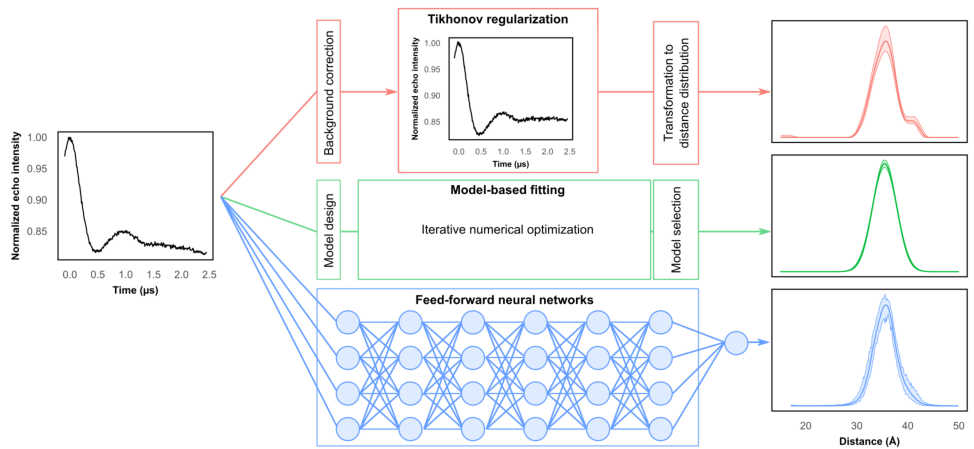
\includegraphics[width=6.5in]{deerintro_methods.pdf}
 \caption[Commonly used methods for analyzing DEER data.]{Commonly used methods for analyzing DEER data.}
\label{fig:deerintro_methods}
\end{figure}

\subsection{Tikhonov regularization}

A widely used approach to stabilizing ill-posed linear problems is to include a penalty term, which is denoted by $L$ and is specific for the problem at hand, that quantifies our expectations of what a reasonable solution should look like. Tikhonov regularization provides a general framework for integrating this penalty term into ordinary least-squares problems \citep*{Tikhonov1963}. The general strategy calculates the optimal probability distribution $\hat{P}$̂ by minimization of both the sum of squared residuals $\norm{KP-S}^2$ and the penalty term $\norm{LP}^2$:

\begin{equation}
    \hat{P}=\underset{P≥0}{\operatorname{\arg \min}} \left\{ \norm{KP-S}^2 + \alpha^2 \norm{LP}^2 \right\}
\end{equation}

Ultimately, the goal of this approach is to generate a smooth distribution with gradual changes in amplitudes between distances fractions of an angstrom apart. For example, it seems unreasonable to expect the peak of a distribution to be at \SI{34.1}{\angstrom} if the probability at \SI{34.0}{\angstrom} is zero. An effective penalty term would therefore restrain the derivative of the distribution, rather than the distribution itself. For this reason, the most widely used matrix penalizes changes in the second derivative \citep*{Edwards2018, FabregasIbanez2019, Jeschke2004}:

\begin{equation}
    L_2 = \begin{bmatrix} 
    1 & -2 & 1 & & & 0 \\
     & 1 & -2 & 1 & & \\
     & & \ddots & \ddots & \ddots & \\
     0 & & & 1 & -2 & 1 \\
    \end{bmatrix}
\end{equation}

This applies the smoothness constraint uniformly throughout the distribution, thus avoiding the spikiness observed by ordinary least-squares fitting. The weight of this term, relative to that of the least-squares term, is determined by the regularization parameter $\alpha$, which does not reflect an experimental variable and is only used to stabilize the probability distribution in solution. In general, lower-quality data require more regularization, and thus larger $\alpha$ values. For any given value of $\alpha$, one of several iterative non-negative least-squares algorithms can be used to obtain an optimal solution \citep*{Bro1997, Lawson1974}.

Not surprisingly, determining the most appropriate value for $\alpha$ is critical to the accurate recovery of distance data. It should be high enough to avoid overfitting noise in the time domain, but no higher than necessary to minimize information loss in the distance domain. Prior to 2018, the most common approach for selecting a value for $\alpha$ was to use an L-curve, in which the distribution is calculated using many values, and the resulting logarithm of the least-squares term of each fit is plotted as a function of the logarithm of the penalty term \citep*{Chiang2005, Jeschke2004}. However, a recent benchmark did not find the widespread practice of selecting the value of $\alpha$ from the “elbow” of this plot to be particularly effective \citep*{Edwards2018}. Instead, the authors proposed using either the \gls{aic} \citep*{Akaike1973} or generalized cross-validation \citep*{Lukas2006}, and since then the use of the former has become standard practice \citep*{FabregasIbanez2020a}. A follow-up study by Fábregas-Ibáñez and Jeschke found that iterative regularization methods can further improve the quality of distributions generated this way \citep*{FabregasIbanez2019}. Although they proposed several alternative approaches to integrate the penalty matrix into the cost function, in practice the Tikhonov functional continues to be widely employed.

As evidenced by its widespread adoption among \gls{epr} spectroscopists, this strategy provides informative distributions without the problems encountered by purely least-squares fitting. Additionally, and in contrast with the model-based paradigm discussed in the following section, it is guaranteed to return the best possible fit given the choice of the penalty matrix $L$ and the regularization parameter $\alpha$. However, its ability to report physiologically meaningful distributions is contingent on the universal application of the smoothness constraint throughout the distribution. As a result, Tikhonov is ill-equipped to handle substantial variation within the distribution, such as mixtures of broad and narrow components, particularly in the presence of noise \citep*{Stein2015}. Sharp components may be smoothed over and broad components may be split. Moreover, artificial peaks may be introduced throughout the distribution to improve the fit, even if there is no physiological basis for their existence \citep*{Casey2015, Jeschke2012}.

One aspect of this optimization approach for the analysis of \gls{deer} data warrants further discussion. The least-squares portion is defined by the matrix-vector multiplication $KP$, effectively preventing the nonlinear background contribution of the \gls{deer} signal from being integrated into this step of the analysis. As a result, the intermolecular coupling signal, modeled by $B \left( t \right)$ as described above, must be determined and removed in advance \citep*{FabregasIbanez2020, Jeschke2004}. This is not a problem when the time collection window is sufficiently large that the intramolecular signal eventually decays to zero, such as when measuring distance distributions that are either short or broadly distributed. Less ideal circumstances may prevent the contribution of background coupling from being readily identified, which can lead to the introduction of fitting artifacts in the distance domain. A secondary result of this \emph{a priori} correction is its effect on the apparent \gls{snr} near the end of the data collection window, termed the “noise explosion” \citep*{FabregasIbanez2020}, which can challenge the assumption fundamental to least-squares fitting that noise values are independently and identically distributed. This can be detrimental to the accurate recovery of short-distance components, and in practice this issue is often sidestepped by signal truncation after background correction. In part to address these concerns, an iterative algorithm was developed that alternates between determining the distribution from the background-corrected data using Tikhonov regularization and refining the background parameter values using nonlinear least-squares fitting \citep*{FabregasIbanez2020a}. The method promises to overcome many of these challenges, but as of writing has not been widely used because of its novelty.

\subsection{Model-based fitting}

The fragmented analytical pipeline required by Tikhonov regularization contrasts with nonlinear least-squares minimization, a one-step approach that can be achieved using a parametric model \citep*{Burnham2002}. The multi-Gauss model, for example, represents the experimental distribution using one or more Gaussian distributions. These parameters, when combined with the background coupling parameters in Equation \ref{eq:deerintro_total}, constitute a parametric model (denoted by $\vartheta$) that can potentially recreate the \gls{deer} signal. As such, their values can be optimized by directly comparing the simulated \gls{deer} trace $V_\mathup{sim} \left( \vartheta \right)$ to the experimental data in the time domain without any background correction:

\begin{equation}
    \hat{\vartheta}=\underset{\vartheta}{\operatorname{\arg \min}} \norm{ V_\mathup{exp} - V_\mathup{sim} \left( \vartheta \right) }^2
\label{eq:deerintro_fitmodel}
\end{equation}

Standard nonlinear optimization algorithms can minimize the deviation between the simulated and experimental DEER traces. These include the Levenberg-Marquardt \citep*{Brandon2012, Levenberg1944, Marquardt1963, Stein2015}, Interior Point \citep*{Hustedt2018, Potra2000}, and Trust Region Reflective \citep*{Byrd1987, FabregasIbanez2020a, Mishra2014} algorithms, as well as approaches such as Hamiltonian \citep*{Hoffman2014, Sweger2020} and random-walk Monte Carlo \citep*{Dzuba2016, Neal1993}, Gibbs sampling \citep*{Edwards2016}, and particle swarm optimization \citep*{Hustedt2018}. Many of the shortcomings discussed above for Tikhonov do not arise with model-based fitting; the background component need not be identified \emph{a priori}, and the use of Gaussian distributions ensures smoothness in the distance domain. Moreover, the only constraint placed upon the model parameters is that the components' amplitudes each exceed zero and total one. This allows the Gaussian mixture model to accurately fit a mix of broad and narrow components that may be challenging for Tikhonov regularization. Finally, the resulting distributions typically lack many of the spurious side peaks and long-distance components that define distributions obtained using Tikhonov and may not be borne out of the signal. 

However, these advantages come at the cost that the best solution is no longer guaranteed to be reached. Whereas linear least-squares problems can be solved analytically, the aforementioned numerical methods required to solve numerical methods may not necessarily converge upon the global minimum. Instead, the solution obtained is the result of iterative improvements of an initial guess provided by the user. Depending on the number of parameters in the model, starting from several unique guesses may be sufficient to identify a reasonable solution \citep*{FabregasIbanez2020a}. A further consideration is the choice of how many Gaussian components constitute the model, which can be guided by several statistical criteria \citep*{Akaike1973, Sugiura1978, Vehtari2017} but must ultimately be chosen by the end user. Collectively, these constraints place a greater burden on the practitioner to avoid the overinterpretation of suboptimal fits.

\section{Structural interpretations of distance distributions}\label{sec:deerintro_globalanalysis}

The intrinsic dynamics and equilibrium states of protein structures come into focus when carrying out multiple orthogonal distance measurements under identical conditions. Proteins may alternate between a discrete number of conformations as part of their function, and the relative proportions of these conformations may be affected by experimental conditions. Whereas an individual \gls{deer} distribution might resemble a featureless smear, a series of measurements in the same pair might reveal distinct distance components that ebb and flow under different conditions. This approach allows discrete conformational states to be extracted from distributions that may otherwise be difficult to interpret. With small datasets and/or simple conformational landscapes, unique conformations can be identified by eye alone \citep*{Barth2018, Duss2014, Kazmier2014a, Manglik2015}.

However, when underlying components are not obvious, specialized approaches may be warranted. In a study of the sodium-coupled aspartate transporter GltPH, which isomerizes between three conformations, eight restraints were measured under six experimental conditions \citep*{Georgieva2013}. These measurements were subsequently fit using three Gaussian components, one for each predicted conformation, under the assumption that the underlying components would retain their means and widths, but change in amplitude. This effort benefited from the determination of several crystal structures in distinct conformations, which provided initial guesses for the distance of each component. This allowed each component across different distance distributions to be linked to specific structures, thus revealing the energy landscape of the transporter. Variations of this approach have been used elsewhere. In a study of HIV-1 protease, the collection of multiple experimental distance distributions allowed the effect of various drugs on specific distance components to be quantified \citep*{Blackburn2009, Casey2015}. Similarly, weighted ensembles of 5-NT in either open, intermediate, or closed conformations were determined under either apo or ligand-bound conditions using a Monte Carlo reweighting approach \citep*{Krug2016}. Again, both cases were aided by a large library of determined conformations.

Similar procedures may nonetheless be carried out even without the information provided by high-resolution protein structures. In their study of the Angiotensin receptor, Wingler \emph{et al} measured ten distance restraints across ten experimental conditions and used \gls{nnmf} to assign specific distance components to four conformations from the entire pool of experimental distance data \citep*{Wingler2019}. Unlike the previous examples, no structures were known \emph{a priori}; in fact, the conformation-specific distances obtained by \gls{nnmf} were ultimately used for molecular dynamics simulations (see Section \ref{sec:deerintro_usingrawdata} below).

Each of these cases relied on distance distributions obtained using Tikhonov regularization to make inferences about a protein's structure and dynamics. As was previously mentioned, Tikhonov can at times introduce artifacts and smooth over sparsely populated components in the distribution. Information lost during analysis cannot be recovered by \gls{nnmf} or Gaussian fitting. One solution is to simultaneously fit the time domain data collected between the same spin-labeled residues under the assumption that certain distance components are conserved across conditions \citep*{Brandon2012}. As with the examples mentioned above, the amplitudes of distinct components will increase and decrease across various conditions, while their means and widths remain fixed. Individual conformations consist of one or more distance components, and their relative energetics can be tracked and monitored under different conditions. The population data obtained this way can reveal details such as the energetics of protein-ligand interactions \citep*{Collauto2017, Dastvan2019} or conformational interconversion \citep*{Dastvan2016a, Jagessar2020, Martens2016, Verhalen2017a}, and facilitate the development of kinetic models of protein function \citep*{Collauto2017, Paz2018}.

\section{Integrative modeling of protein structures using DEER data}

The previous sections discussed the challenges of transforming one-dimensional data in the time domain to one-dimensional distributions in the distance domain. The remainder of this chapter discusses the more daunting task of converting multiple distance distributions into detailed models of protein structures and ensembles. If properly executed, the integration of these data with modeling can reveal the binding and interaction interfaces of multiple proteins or subunits, the conformational heterogeneity of protein substructures under different conditions, and even the topology or fold of protein structures that have not been previously determined to high resolution. 

\subsection{General principles of integrative modeling using experimental data}\label{sec:deerintro_general_integrative}

Quantitative models aim to explain or justify past observations, and/or predict future observations \citep*{Hofman2021}. Several recent reviews focused on integrative modeling of protein structures \citep*{Rout2019, Sali2021} have outlined five possible uses for experimental data: 

\begin{enumerate}
    \item \textbf{Choosing a representation of the protein structure.} In the context of \gls{deer} data, which reports distance distributions between flexible spin labels, atomic-detail information is unavailable. Thus, absent other sources of experimental information, only low-resolution fold-level models are generally feasible.
    \item \textbf{Scoring candidate structural models.} A model's agreement with experimental data must be quantified for direct comparison to other models.
    \item \textbf{Constraining the search space.} Given both the complexity of protein structures and the fundamental sparseness of the \gls{deer} data, exhaustive searches of the fold space are impossible. This is closely related to the choice of which sampling method to use \citep*{Maximova2016}.
    \item \textbf{Filtering of models after sampling.} Agreement with experimental data may be use to filter models \emph{ex post facto}, which is often necessary if consistency with experimental data cannot be rapidly quantified.
    \item \textbf{Model validation.} Finally, the soundness of structural models can be verified using experimental data that may be difficult to quantitatively incorporate.
\end{enumerate}

Most recent advancements surrounding the integration of \gls{deer} data into modeling pipelines can be categorized as improvements in either scoring or filtering approaches. Nevertheless, all modeling studies must first address how to adequately constrain the search space.

%However, whereas most widely used structural biology methods directly report the positions of the atoms comprising the protein structure, \gls{deer} instead reports distance distributions between flexible spin labels attached to the protein structure. Although the spin label facilitates the determination of the protein's structure, its position is rarely of interest to the structural biologist. As a result, two fundamental challenges prevent atomic-detail structural models from being accurately and reliably obtained with \gls{deer} data. First, atomic-detail structural models are largely unachievable as insufficient data is available to restrain such models. Second, current computational methods can rarely reproduce experimental distance data from the target structure of interest, adding further uncertainty when translating experimental measurements into computational models.

\subsection{Working with sparse data}

Even the smallest proteins contain thousands of atoms, and even the coarsest depictions must account for at least two rotatable bonds per residue. If a model can sample these degrees of freedom without restriction, then the \gls{deer} technique's low throughput all but ensures that model parameters outnumber distance restraints (Figure \ref{fig:deerintro_complexity}). The problem can be simplified if the structures of certain regions are known and forced to remain static: rigid body docking of $N$ discrete domains has $6(N-1)$ degrees of freedom \citep*{Duss2015}, or $4(N-1)$ for symmetric homooligomers \citep*{Hilger2007}. Indeed, countless examples exist in the literature of \gls{deer} data being used to identify either a docking interface or the relative spatial arrangements of multiple domains. As an added benefit, the search space of the problems shrinks to the point that it may be searched nearly exhaustively \citep*{Alonso-Garcia2015, Kim2011, Sundaramoorthy2017}.

If intradomain movement cannot be ruled out, then soft restraints can be used to limit the extent to which a model reconfigures away from a known conformation. For example, Evans \emph{et al.} modeled a conformational change in SthK by restraining $\mathrm{C_{\upalpha}}$ atoms to distances observed in the starting conformation using a sigmoid-like function that increased the penalty of deviations up to but not beyond \SI{1}{\angstrom} \citep*{Evans2020}. This limited the changes introduced to the model to regions that were inconsistent with the experimental data. Alternatively, the source of the conformational change can be determined by eye. Kazmier \emph{et al.} found that conformational changes in the transporter LeuT predominately map to four transmembrane helices. This allowed the remainder of the protein structure to be restrained, preventing unnecessary movement \citep*{Kazmier2014a}. Finally, such restraints can be introduced implicitly, such as by starting from a template \citep*{Binder2019, Evans2020}.

Without prior structural information, \gls{deer} distance restraints play a supplementary role to either energy functions and/or alternative sources of experimental data such as \gls{nmr} restraints. Their integration is discussed in Section \ref{sec:deerintro_main_integration}.

\begin{wrapfigure}{R}{0.4\textwidth}
\centering
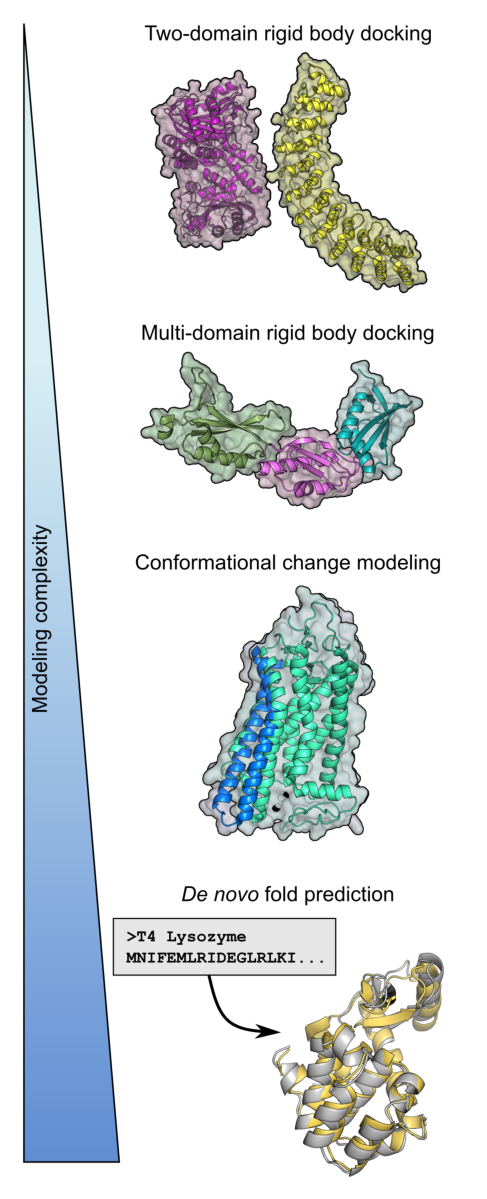
\includegraphics[width=2.5in]{deerintro_complexity.pdf}
 \caption[Protein modeling applications ranked by complexity.]{Protein modeling applications ranked by complexity. More complex problems, such as fold prediction or homology modeling, generally require more restraints to obtain accurate.}
\label{fig:deerintro_complexity}
\end{wrapfigure}

\section{Evaluating a model's agreement with experimental DEER data}

\subsection{Simulation of nitroxide side chains}\label{sec:deerintro_rotamers}

Accurately modeling a protein structure is only possible when the target conformation recapitulates the experimental data more effectively than alternative conformers. The reliance on flexible spin labels complicates the problem of identifying the conformer of interest using \gls{deer} data. Distances are measured between stably bound unpaired electrons far from the protein backbone; for example, in the widely used \gls{mtssl}, they are separated from the $\mathrm{C_{\upbeta}}$ atom by \SI{6}{\angstrom} and five $\upchi$ angles. Ultimately the linkers anchoring these unpaired electrons to the protein backbone determine how distances between unpaired electrons relate to distances between backbone atoms. Their conformations are generally not known in advance (although they can be determined using specialized algorithms, discussed in Section \ref{sec:deerintro_usingrawdata} below). Therefore, accurate models of protein structures require accurate distance distributions, which in turn require accurate predictions of spin labels rotamers.

However, the introduction of spin labels into the protein model is not straightforward. For example, several problems become apparent even in simple cases where protein structures being simulated in an MD environment are modified to have nitroxides at residues that have been experimentally labeled \citep*{Borovykh2006, Bowman2009, Brown2002, Corey2019, Hays2019, Islam2015, Islam2013, Marinelli2015, Marinelli2019, Roux2013}. First, whereas the two spin labels attached to any individual experimentally expressed double-cysteine mutant are unlikely to clash, an \emph{in silico} model attempting to integrate data from many \gls{deer} experiments may contain many explicitly modeled nitroxide side chains, some of which may be in close proximity to one another \citep*{Islam2013}. Second, the identity of the residue being labeled can provide valuable modeling information about which environments it preferentially occupies \citep*{Alexander2008}. For example, mutation of a tryptophan in a membrane protein to a nitroxide prevents it from informing the simulation software about structural characteristics such as membrane depth. Finally, and perhaps most critically, the computational cost of atomic-detail molecular dynamics simulations precludes its use as a screening tool that quantifies any given structural model's agreement with \gls{deer} data.

\Gls{mc} modeling paradigms provide one alternative approach. In this modeling paradigm, the spin label configurations are randomly picked from rotamer libraries, the probabilities of which are computed in advance. However, whereas rotamer statistics for canonical amino acids can be obtained directly from the PDB, those for nitroxide spin labels must instead be computed from detailed quantum mechanical calculations, a procedure described in detail elsewhere \citep*{Alexander2013, Edwards2014, Polyhach2011, Schmidt2015, Yang2020}. After obtaining these rotamers, \gls{mc} facilitates the rapid sampling a residue's local environment, and pairwise measurements can then be compared to experimental distances. The accuracy of distances obtained this way is comparable to those obtained by traditional \gls{md} \citep*{Klose2012} and in many cases are able to recover the rotamers observed experimentally \citep*{Alexander2013}. However, \gls{mc} methods have the advantage of being several orders of magnitude faster.

MDDS, an alternative developed by Islam and Roux, allows \gls{md} methods to rapidly calculate distance distributions from protein models in minutes to hours while avoid modeling spin labels to atomic detail \citep*{Islam2013}. By using a set of over fifty experimental distance restraints collected in T4 Lysozyme, they generalized the position of the unpaired electron with respect to the protein backbone. They then converted these positions into force fields between backbone atoms and a dummy atom representing the unpaired electron, allowing them to discard the rest of the nitroxide side chain.

\subsection{Simulation of DEER distance distributions}

Whereas experimental distance measurements are carried out between ensembles of molecules, computational methods generally model only a single structure at a time. To model the distribution of distance measured in ensembles of molecules, MDDS uses large numbers of noninteracting dummy atoms to build distance distributions \citep*{Kazmier2014a, Raghuraman2014}. Marinelli and Faraldo-Gomez instead used a time window to build their distributions from \gls{md} simulations between explicit nitroxide rotamers \citep*{Hustedt2018, Marinelli2015, Marinelli2019}. Alexander \emph{et al.} generated thousands of models using full-atom MC modeling and assembled distributions from those with the lowest energy \citep*{Alexander2013}.

By far the most common strategy in the literature models ensembles of possible nitroxide conformations. Methods such as MMM \citep*{Jeschke2018, Polyhach2011}, Pronox \citep*{Hatmal2012}, Nasnox \citep*{Beasley2015, Price2007, Tangprasertchai2015} and TagDock \citep*{Edwards2014} introduce every possible configuration stored in of a rotamer library one at a time and calculate Boltzmann energy values for those that do not clash with the rest of the protein. Some methods, such as TagDock, allow neighboring side chains to be repacked in response \citep*{Edwards2014}; others, such as MMM, can be applied to individual frames within an \gls{md} simulation to visualize the contribution of backbone dynamics \citep*{Stelzl2014, Tesei2020}. By contrast, MtsslWizard \citep*{Hagelueken2013, Hagelueken2012} uses \gls{mc} to sample rotamers until the number of either accepted rotamers or clashes reaches a predetermined threshold. A benchmark by Klose \emph{et al.} established that distributions simulated using these rotamer libraries are comparable in accuracy to those simulated using \gls{md}, with the distribution's average values deviating by about \SI{3.0}{\angstrom} from those observed experimental in each case \citep*{Klose2012}.

However, neither this approach, nor to our knowledge \gls{md}, can simulate distributions with widths that correlate with experimental values \citep*{Jeschke2013}, with the former consistently overstating spin label dynamics while neglecting backbone dynamics \citep*{Dastvan2016}. The only method that has achieved any correlation with experimental widths is a sampling-intensive \gls{mc} refinement approach that permits changes in the protein backbone \citep*{Alexander2013}, which suggests that coupling of backbone and side chain dynamics in solution may contribute to the width and shape of experimental distance distributions. Such a case has been crystallographically observed in the chaperone Spa15 when a loop containing a spin-labeled residue was found to slightly reconfigure compared to the wildtype structure \citep*{Lillington2011}.

One explanation for this discrepancy between experimental and simulated distribution widths is the fact that \gls{deer} measurements are almost always carried out in protein samples following the addition of cryoprotectants (such as glycerol) and flash-freezing. The common practice of submerging microliter-volume samples in liquid nitrogen gives spin labels up to hundreds of milliseconds to reconfigure and converge upon low-energy conformers \citep*{Schmidt2020}. Studies with T4 Lysozyme \citep*{Georgieva2012} and hemoglobin \citep*{Banham2007} have observed that the speed at which a sample freezes affects the width of the resulting experimental distribution. It is unclear if this effect could be corroborated \emph{in silico}, since the timescales of such a simulation are not currently feasible. Most likely, the experimental distribution likely involves a complex interplay between the spin label's local environment, the sample conditions and choices involved in its preparation, and the speed at which the sample was frozen.

\subsection{Scoring functions}\label{sec:deerintro_scoring_fxns}

How can the target conformation be identified if it cannot be expected to recreate the experimental data? Unfortunately, no consensus exists on this topic in the literature. Average values of distributions are widely used for the simple reason that their values correlate reasonably well with computational predictions made from structural models. As was just discussed, distribution widths cannot be recapitulated and are frequently ignored altogether, while distribution shapes are far more difficult to glean from the raw data and as a consequence rarely factor into modeling.

One strategy that has seen relatively widespread use is to model the nitroxide rotamers using a rotamer library such as MMM and to measure distances from the unpaired electron closest to the ensemble average \citep*{Dastvan2016, Duss2014, Duss2015, Duss2014a, Fehr2015, Raba2014, Ward2009}. Comparing these distance values to experimental averages allows a model to be scored using the sum of squared residuals. This retains the benefits of using the entire ensemble of spin label conformations while removing potentially unreliably information from the distance distribution. Nevertheless, alternative scoring functions sometimes are used that factor the width of the distribution. For example, in several studies, the deviation between the simulated and experimental average values has been divided by the experimental distribution's width. Presumably, this accounts for backbone heterogeneity by less aggressively penalizing deviations between residues with wider distributions \citep*{Jeschke2016, Peter2019}, although to our knowledge no benchmarks have been carried out to ascertain the merit of this fact. Alternatively, the entire shape can be retained, and the score of a model can be either its percent overlap \citep*{Hays2019, Jeschke2020, Kazmier2014a, Raghuraman2014} or the area between the integrals of the two distributions \citep*{Krug2016}.

It is important to note that regardless of the scoring function, the spin label's flexibility means that the direct application distance restraints to the unpaired electron or nitroxide bond to be largely ineffective at obtaining high-precision protein models, as the rotamers can easily reconfigure without any backbone changes. For example, when dummy atoms are used to model conformational changes modeled using MDDS, they have been found to absorb changes in the distance distribution, leaving the backbone untouched \citep*{Kazmier2014a, Raghuraman2014}. Applying distance restraints to the nitroxide bond of the rotamers in an MC simulation is fraught with similar challenges: for example, Herrick \emph{et al.} constrained the first two chi angles of \gls{mtssl} after finding that rotamers would otherwise adopt "unrealistic orientations" \citep*{Herrick2009, Lai2011}. Similar observations were made when modeling 5-NT \citep*{Krug2016} and Omp85 \citep*{Dastvan2016}. An exception is when data has also been collected using \gls{pre} paramagnetic relaxation enhancement \gls{nmr}, which measures distances between an unpaired electron and backbone nuclei. These distance data can be used as additional restraints on nitroxide rotamers to prevent them from reconfiguring \citep*{Milikisiyants2017, Saio2021, Wu2013}. However, the rotamers that contribute to the experimental signals may differ between the two datasets, since \gls{deer} samples are measured after flash-freezing whereas \gls{pre} samples are measured at room temperature.

\subsection{Limits of modeling protein structures using explicitly modeled rotamers and rotamer libraries}

Distance distributions in non-\gls{md} environments can typically be simulated in seconds or tenths of a second, with the majority of computation time typically devoted to calculating clashes with the rest of the protein. Unfortunately, even these speeds still preclude the use many modeling applications. Most studies therefore use these methods to screen models \emph{ex post facto}, rather than restrain them directly during sampling. Some studies circumvent these cost restrictions by introducing rotamers prior to modeling and retaining them throughout sampling without recalculating clashes, thus skipping the most computationally expensive step. Such a strategy was appropriate when docking CDB3 and Ankyrin \citep*{Edwards2014}, as the local environment of the spin labels were not expected to change throughout the docking simulation. Alternatively, a number of studies only retain the rotamer closest to the center of the ensemble: by fixing it in space relative to the backbone, it could be restrained using distance data without risking its reconfiguration \citep*{Bibow2017, Duss2014, Duss2014a, Raba2014,  Ward2009}.

\subsection{Direct integration of DEER data during sampling using restraints between backbone atoms}\label{sec:deerintro_main_integration}

Because of this computational cost issue, these data are more frequently integrated as restraints between backbone atoms during sampling. Restraints between $\mathrm{C_{\upbeta}}$ atoms are more common, although $\mathrm{C_{\upalpha}}$ atoms have also been used \citep*{Park2006, Sale2004}. While trivial to implement in most modeling packages, this approach requires that distance values between spin labels be transformed into distance restraints between backbone atoms. Unfortunately, these measurements do not always line up perfectly \citep*{Hirst2011}. Yang \emph{et al.} demonstrated the danger of taking these experimental distances at face value when predicting the structure of the homodimer Dsy0195 \citep*{Yang2010}. The \gls{rmsd} of their model improved when using a restraint with an experimental \gls{deer} distance that matched the $\mathrm{C_{\upbeta}}$-$\mathrm{C_{\upbeta}}$ distance, but worsened when the two values differed by as little as \SI{5}{\angstrom}. As has been previously noted \citep*{Alexander2008, Bhatnagar2007, Borbat2002, Fischer2016, Georgieva2013, Jeschke2013, Sale2005}, deviations of this magnitude are not uncommon. In globular proteins, spin labels tend to face away from each other, leading to experimental distances values that exceed the corresponding $\mathrm{C_{\upbeta}}$-$\mathrm{C_{\upbeta}}$ distance by a median of \SIrange{6}{7}{\angstrom}. By contrast, the deviations between these values across protein-protein interfaces are lower but nonetheless significant \citep*{Bhatnagar2007, Fischer2016, Kim2011}. Notably, these values exceed the \SI{3}{\angstrom} deviation observed between the average values of simulated and experimental \gls{deer} distance distributions, highlighting the loss of precision that comes with this scoring approach \citep*{Sale2005}.

Backbone potentials frequently score a model's agreement with experimental data using wide and flat-bottomed harmonic potentials. These have be introduced as NOE-like restraints into programs such as CYANA \citep*{Guentert2004}, Xplor-NIH \citep*{Schwieters2003}, CNS \citep*{Brunger1998}, Rosetta \citep*{Leaver-fay2011, Leman2020, Simons1997}, and BCL \citep*{Karakas2012, Woetzel2012}. Both Alexander \emph{et al.} and MacCallum \emph{et al.} successfully predicted the structures of T4 Lysozyme and aA-crystallin \emph{de novo} using this type of restraint \citep*{Alexander2008, MacCallum2015}. In both cases, a score of zero was assigned to $\mathrm{C_{\upbeta}}$-$\mathrm{C_{\upbeta}}$ distances (in angstroms) ranging from $\upmu_\mathit{SL} - \upsigma_\mathit{SL} - 12.5$ to  $\upmu_\mathit{SL} + \upsigma_\mathit{SL} + 2.5$, where $\upmu_\mathit{SL}$ and $\upsigma_\mathit{SL}$ are the average values and standard deviations of the experimental distribution. Similarly, Kim \emph{et al.} determined the docking interface of CDB3 and Ankyrin using a criterion in which any model was kept if its $\mathrm{C_{\upbeta}}$-$\mathrm{C_{\upbeta}}$ distances deviated by less than \SI{14}{\angstrom} from the experimental average distance \citep*{Kim2011}. Alternatively, the edges of the distribution have been used as restraints bounds \citep*{Bibow2017}.

These scoring functions, although broad, can nonetheless respond poorly to outliers. Bhatnagar \emph{et al.} noted when docking CheA and CheW that a pair of $\mathrm{C_{\upbeta}}$-$\mathrm{C_{\upbeta}}$ restraints whose distance deviated substantially from experimental interspin distance values prevented low-\gls{rmsd} models from being obtained; their removal improved the \gls{rmsd} of the docking interface from over \SI{10}{\angstrom} to \SI{2.6}{\angstrom} \citep*{Bhatnagar2007}. However, they used a more restrictive potential with lower and upper bounds of $\upmu_\mathit{SL} -$\SI{5.0}{\angstrom} and $\upmu_\mathit{SL} +$\SI{1.0}{\angstrom}, respectively, which may increase the scoring function's sensitivity to outliers \citep*{Bhatnagar2010}.

A similar strategy was employed by Evans \emph{et al.} when modeling conformational changes in the ion channel SthK \citep*{Evans2020}. They took advantage of a starting conformation, as well as a set of \gls{deer} data for that conformation, by applying the magnitude of the distance change as a harmonic restraint between $\mathrm{C_{\upbeta}}$ atoms with a lower and upper bound of $\upmu_\mathit{SL} -$\SI{1.0}{\angstrom} and $\upmu_\mathit{SL} -$\SI{1.0}{\angstrom}, respectively. This strategy has the benefit of reducing variation among generated models but assumes that domains and spin labels do not rotate or substantially reconfigure with respect to one another.

Hirst \emph{et al.} generated a custom cubic spline function called the \gls{cone} model that, unlike a flat-bottomed harmonic function, accounts for the fact that the experimental distance is more likely, but not necessarily guaranteed, to be longer than the $\mathrm{C_{\upbeta}}$-$\mathrm{C_{\upbeta}}$ distance \citep*{Hirst2011}. Its use improved the number of high-resolution models folded \emph{de novo} for T4 Lysozyme, and it has since been applied to problems involving \emph{de novo} folding \citep*{Fischer2015, Fischer2017, Fischer2016}, docking \citep*{Alexander2014, Dastvan2016, Fischer2016, Tessmer2018}, and conformational change modeling \citep*{Dastvan2016, Kim2012, Krug2016, VanEps2011}.

None of these approaches can determine unequivocally the structures of proteins or complexes. For example, Kim \emph{et al.} found that the incorporation of twenty experimental restraints when docking CDB3 and Ankyrin led to a wide range of possible configurations \citep*{Kim2011}. This highlights the breadth of the solution space, even in cases where the experimental restraints outnumber the degrees of freedom by more than threefold. Ultimately this pool of models was further trimmed using an orthogonal set of \gls{epr} data that measured the solvent accessibility of individual spin-labeled residues.

This hierarchical approach contrasts with the direct integration of flat-bottomed harmonic restraints into sampling, which has the intended effect of directing the modeling protocol to a conformational subspace encompassing the target structure. Optimization within this subspace proceeds using additional criteria, such as energy functions or experimental \gls{nmr} restraints, which can evaluate structural features with greater precision. The MELD structure prediction program, for example, navigates this subspace using AMBER forcefields and replica exchange molecular dynamics \citep*{MacCallum2015, Perez2016}, whereas Rosetta relies on its coarse-grained energy function and \gls{mc} sampling \citep*{Alexander2008, Kazmier2011}. By contrast, Ling \emph{et al.} used Xplor-NIH to model the structure of YagP by combining \gls{deer} data with \gls{epr} membrane depth restraints \citep*{Ling2016}. In each case, the flat-bottomed potentials do not interfere with optimization within this region; instead, they guide the conformational search away from false minima that fall outside their bounds. As a result, the weights of these restraints, relative to other experimental restraints or score terms, is not generally optimized or fine-tuned. 

By contrast, the \gls{cone} model developed by Hirst \emph{et al.} does introduce a bias into the search procedure by assuming that the experimental distance will usually, but not always, exceed the $\mathrm{C_{\upbeta}}$ distance. This assumption modifies the function landscape and must therefore be carefully integrated into the modeling protocol. During the development of this energy potential, Hirst \emph{et al.} determined by grid search a weight for this energy potential that maximized the proportion of high-accuracy models of T4 Lysozyme. This weight has since been used in virtually all cases outlined above.

We note that although these restraints are imprecise, they are often followed by the use of higher-precision scoring functions in conjunction with atomic-detail depictions of spin label rotamers more amenable to the identification of accurate models \citep*{Sarver2018}. For example, structural modeling of EmrE was achieved using the \gls{cone} model in BCL::Fold followed by refinement with Modeller using the rotamer libraries available in MMM \citep*{Dastvan2016}. The structure of the C-terminus of ExoU was similarly modeled \emph{de novo} using the \gls{cone} model, followed by \emph{in silico} spin labeling with explicit \gls{mtssl} side chains using Rosetta \citep*{Fischer2017}. The CheA/CheW binding interface was determined by generating a set of initial models using $\mathrm{C_{\upbeta}}$-$\mathrm{C_{\upbeta}}$ restraints followed by finer-grain selection using rotamer libraries \citep*{Bhatnagar2007}. Thus, the use of coarse backbone restraints can set the stage for finer-grain modeling.

\subsection{Error analysis}

Our discussion has extensively mentioned the limit of \gls{deer} restraints in modeling structures: even docking interfaces cannot be determined with absolute certainty using these data. Fortunately, quantification of the uncertainty of these models is increasingly widely used. Cross-validation requires that multiple subsets of these restraints be used for modeling, and the results compared to check the stability of the solutions. This approach has been used to model the NhaA homodimer \citep*{Hilger2007}, 5-NT \citep*{Krug2016}, and RmsE/RmsZ \citep*{Bhatnagar2007}. The docking interface of the NhaA homodimer, for example, was determined using each of the 36 available combinations of seven restraints from nine restraints available, leading to an \gls{rmsd} of \SI{0.45}{\angstrom} among each of the thirty-six best models from each set \citep*{Hilger2007}. Bowen and colleagues took this idea a step further and quantified the uncertainty resulting from the choice of rotamer library \citep*{Bowen2018}. Alternatively, if a starting structure is available, the error calculated for that structure can be used to inform the precision with which certain features and/or substructures of a protein can be modeled with high confidence. Bliecken \emph{et al.} calculated the deviations among restraints in the soluble Bax monomer, which had been initially determined using \gls{nmr}, and used those values to inform the accuracy of their model for the membrane-bound Bax dimer \citep*{Bleicken2014}. More commonly, uncertainty is depicted informally, for example by presenting a handful of the best-scoring models \citep*{Evans2020, Gigli2018, Kim2011}. Far more often it is ignored altogether.

\subsection{Integrating DEER restraints with other types of experimental data}

Flat-bottomed harmonic functions, although imprecise, nonetheless allow DEER data to be elegantly integrated into a modeling protocol involving other types of data. When modeling distributions using programs such as MMM, it is less clear how best to jointly consider agreement with both \gls{deer} data and, for example, \gls{saxs} data. One option mentioned above is to use hierarchical approaches, where models are effectively filtered out if they fail to satisfy each of several experimental criteria. Bowman, Boura, and Sundaramoorthy combined \gls{deer} and \gls{saxs} data using this approach for rigid-body modeling of Vps75/Nap1, ECSRT-I, and Chd1, respectively \citep*{Boura2012, Boura2011, Bowen2018, Sundaramoorthy2017}. In each case, models needed to be docked in such a way that both the \gls{deer} data and \gls{saxs} density were satisfied. Several examples in the literature exist in which this is done informally, such that a solution obtained using \gls{deer} data is simply validated using experimental data from another source. Hilger \emph{et al.} compared their model for the dimeric NhaA antiporter to previously published low-resolution 2-D cryo-electron microscopy data \citep*{Hilger2007}, whereas Sung \emph{et al.} docked their model of Bax into \gls{saxs} density \citep*{Sung2015}.

A preferable approach is the direct integration of the two during sampling. This, however, requires that scores be balanced in such a way that avoid overemphasizing data from either method. To our knowledge, no single widely used approach exists. In the literature, ESCRT-II was modeled using both \gls{saxs} and \gls{deer} data using a $\chi^2$ potential for each experimental technique \citep*{Boura2012}. Peter \emph{et al.} also used $\chi^2$ potentials to model YopO using both \gls{saxs} and \gls{deer}, but simply compared the average values of the simulated and experimental distributions \citep*{Peter2019}.

\subsection{When simulation guides experiment: choosing restraints using starting structures}

Several application-specific algorithms have been developed that recommend experimental restraints. These recommendations are typically application-specific, as the demands of each application change the information being sought by the experimental data. As an example, \emph{de novo} folding problems benefit from restraints between residues that are distant in sequence but close in space. The \gls{mc} algorithm developed by Kazmier \emph{et al.} that chooses restraints for \emph{de novo} folding uses two criteria: it tries to ensure that the pairs of residues are far apart in sequence space while diversifying their placements to avoid collecting redundant information, for example between the same pair of helices \citep*{Kazmier2011}. By contrast, when a structure is known but its loops are not, networks of four restraints per spin-labeled loop residue have been proposed in a procedure analogous to triangulation \citep*{Jeschke2016}. For conformational change problems, both Hays \emph{et al.} \citep*{Hays2018} and Mittal and Shukla \citep*{Mittal2017} developed restraint-picking methods for conformational change modeling problems that prioritize the reduction of redundant information by selecting residue pairs whose movements are minimally correlated; both rely on short nanosecond \gls{md} simulations to obtain an initial guess for these structural dynamics. If for some reason such a simulation is impossible, an alternative method \citep*{Jeschke2012a} predicts which regions of a protein structure will move using normal mode analysis and a modification of the Zheng-Brooks algorithm \citep*{Zheng2005}. The same author proposed a separate criterion for rigid body docking problems, which require far fewer restraints to define analytically \citep*{Jeschke2020}. Since only three residues need to be spin labeled per rigid body, an intuitive choice is to choose the three residues in each rigid body that generate the largest nearly-equilateral triangle. This minimizes the propagation of errors throughout the docked structure.

\section{Towards the analysis of DEER data by structural modeling}\label{sec:deerintro_usingrawdata}

The first half of this chapter discussed the difficulty of extracting distance data from \gls{deer} traces in the time domain, while the second half discussed how best to use those distance data for modeling protein structures. In principle, the two steps can be directly integrated by attempting the simulate the raw data using the same approach summarized earlier. Briefly, the conformation determines the distance distributions being fitted and reconfigures to improve the goodness-of-fit in the time domain. Several studies have attempted to recapitulate the raw data from protein models as early as 2007 \citep*{Bhatnagar2007, Hilger2007}. The previously mentioned ESCRT-II, which was modeled using the raw \gls{deer} traces alongside \gls{saxs} data using a $\chi^2$ potential to balance the two \citep*{Boura2012, Boura2011}. Marinelli and Fiorin modeled a conformational change in VcSiaP by restraining the spin labels directly using the raw data \citep*{Marinelli2019}. Notably, both the study of VcSiaP and NhaA also attempted to fit the background contribution to the signal, which was added to the simulated data using a "fit-within-a-fit" procedure. By contrast, the study of ESCRT-II, as with others \citep*{Reichel2018}, background-corrected the data before using it as a restraint.

Additionally, we mentioned in this chapter that native or correctly folded models are not expected to perfectly recapitulate the experimental \gls{deer} distance distribution. Failure to account for this expectation can cause the data to be overfitted. In fact, whereas this expectation can easily be encoded into the scoring function when scoring models using data in the distance domain - for example, using broad, flat-bottomed functions (see Section \ref{sec:deerintro_scoring_fxns} above) - it is far more difficult to anticipate the magnitude of these deviations in the time domain. This imprecision prevents minor contributions to the experimental signal from being resolved, removing one of the fundamental advantages of the \gls{deer} technique.

How can this issue be addressed? One might intuit that less flexible spin labels, the positions of which can more precisely be simulated from the backbone, may be positioned to improve the precision of simulated distributions enough to permit modeling using data in the time domain. Several options are explored in the literature. The label IDSL (also called V1 or RSSR), for example, has far less rotameric freedom than \gls{mtssl} and leads to sharper distance distributions \citep*{Balo2016, Warshaviak2013}. Other alternatives that have been used for modeling include bifunctional spin labels \citep*{Fajer2015, Islam2015, Sahu2017} and paramagnetic copper ions \citep*{Cunningham2015, Merz2014} that are conjugated to or coordinated by pairs of alpha carbons. By reducing or altogether eliminating the contribution of rotamer dynamics to the width of the distribution, these methods can potentially isolate the contribution of backbone dynamics. Moreover, it avoids the risk of uncritical accepting the width of the rotamer distribution obtained from methods such as MMM, which may cause backbone dynamics to be understated (see Section \ref{sec:deerintro_rotamers}).

A second option to reduce uncertainty is to determine the positions of flexible spin labels in advance. This triangulation procedure, however, requires a conformation of the protein to be known \emph{a priori} that is consistent with a set of experimental data. The positions of the spin labels can be determined by singular value decomposition  \citep*{Hagelueken2013}, non-linear least squares minimization \citep*{Bleicken2014}, or by eye \citep*{Wingler2019}. An instructive example is provided in the study of the Angiotensin receptor, where distance distributions attributed to a known conformation were used to determine which rotamers were sampled in solution\citep*{Wingler2019}. The distance data from other conformations were then used for conformational change modeling using \gls{md}. Similarly, the model of dimeric membrane-embedded Bax was obtained by first determining the \gls{mtssl} rotamers from the monomeric model \citep*{Bleicken2014}. However, the constraints placed upon rotamer triangulation - that a conformation is both known to high resolution and consistent with a set of experimental data - make it uncommon, and this technique has not yet been used to model proteins using data in the time domain. More often, it is used to localize a paramagnetic ligand or ion within the same structure \citep*{Gaffney2012, Yang2012}.

What would the key benefit be of working with the raw data? To answer this question, it may be prudent to take a global perspective on the state of the art, as outlined in Section \ref{sec:deerintro_deeranalysis} above. \Gls{deer} data are commonly background corrected, then analyzed; \gls{deer} distance distributions are partitioned among several conformations, with the average peak of each component frequently isolated for the purposes of modeling. As discussed above, information lost during each of these four steps cannot later be recovered. It may, however, be accessible to one-step approaches that simulating the raw data from an ensemble of models. It is in precisely this direction that we hope the field moves.
\clearpage % clear the prior chapter's page

\chapter{Rapid simulation of unprocessed DEER decay data for protein fold prediction}\label{ch:rosettadeer}
%\vspace{-7mm}
%\bigskip

The contents of this chapter have been previously published \citep*{DelAlamo2020}.

\bigskip

Despite advances in sampling and scoring strategies, Monte Carlo modeling methods still struggle to accurately predict \emph{de novo} the structures of large proteins, membrane proteins, or proteins of complex topologies. Previous approaches have addressed these shortcomings by leveraging sparse distance data gathered using \gls{sdsl} and \gls{epr} spectroscopy to improve protein structure prediction and refinement outcomes. However, existing computational implementations entail compromises between coarse-grained models of the spin label that lower the resolution and explicit models that lead to resource-intense simulations. These methods are further limited by their reliance on distance distributions, which are calculated from a primary refocused echo decay signal and contain uncertainties that may require manual refinement. Here, we addressed these challenges by developing RosettaDEER, a scoring method within the Rosetta software suite capable of simulating \gls{deer} distance distributions and decay traces between spin labels fast enough to fold proteins \emph{de novo}. We demonstrate that the accuracy of resulting distance distributions match or exceed those generated by more computationally intensive methods. Moreover, decay traces generated from these distributions recapitulate intermolecular background coupling parameters, even when the time window of \gls{epr} data collection is truncated. As a result, RosettaDEER can discriminate between poorly folded and native-like models using decay traces that cannot be accurately converted into distance distributions using regularized fitting approaches. Finally, using two challenging test cases, we demonstrate that RosettaDEER leverages these experimental data for protein fold prediction more effectively than previous methods. These benchmarking results confirm that RosettaDEER can effectively leverage sparse experimental data for a wide array of modeling applications built into the Rosetta software suite.

\section{Introduction}

Structural biology increasingly relies on integrated methods to model the structure and dynamics of proteins and protein assemblies \citep*{Steven2008, Xia2017}. Multiple complementary experimental methodologies can describe the structure and dynamics of proteins that elude determination from a single technique, such as integral membrane proteins, conformationally flexible proteins, and those that fall outside the size limitations of solution-state nuclear magnetic resonance and \gls{cryoem}. By integrating experimental data from multiple approaches, computational modeling can build accurate models in regions with sparse experimental data. One promising source of high-resolution experimental data for integrated structural biology combines \gls{sdsl} and \gls{epr} \citep*{Jeschke2018a, Sahu2018}. Previous studies have employed \gls{sdsl}-\gls{epr} and computation in tandem to predict protein structures \emph{de novo} \citep*{Alexander2008, Fischer2015, Fischer2017, Fischer2016, Hirst2011, Kazmier2011, Ling2016, Yang2010}, model conformational changes \citep*{Kazmier2014, Kazmier2014a, Marinelli2019, Raghuraman2014}, and dock rigid-bodies \citep*{ Bhatnagar2007, Edwards2014, Hilger2007}.

Existing modeling methods largely focus on data gathered using four-pulse \gls{deer} \citep*{Pannier2000}, which can report on distances of up to \SIrange{60}{80}{\angstrom} between stable unpaired electrons conjugated to the protein backbone by \gls{sdsl} \citep*{Jeschke2012, Mchaourab2011}. However, incorporation of these distances as interatomic restraints for modeling purposes is confounded by the conformational freedom of these paramagnetic probes. The central challenge is to convert inter-spin distance information into structural restraints that report on the protein backbone \citep*{Abdullin2016, Alexander2014, Iwahara2004}. Additionally, the need to incorporate two spin labels into the protein sequence per restraint results in sparse coverage of the experimental data that can introduce ambiguities into computational modeling \citep*{Kazmier2011}. As a result, only a few experimental restraints are generally available to describe the protein fold.

These sparse datasets have nonetheless been leveraged for protein structure prediction and refinement by a range of computational modeling approaches that represent the spin labels either implicitly or explicitly. Implicit models such as the \gls{cone} model \citep*{Alexander2008} use knowledge-based potentials to translate inter-spin distance values into backbone restraints, typically between $\mathrm{C_{\upbeta}}$ atoms \citep*{Sale2005}. Introducing these restraints led to measurable improvements in \emph{de novo} structure prediction benchmarks by programs employing Monte Carlo sampling strategies \citep*{Alexander2008, Fischer2015, Fischer2017, Fischer2016, Hirst2011, Kazmier2011}, gradient minimization \citep*{Ling2016, Yang2010}, and molecular dynamics \citep*{MacCallum2015}. However, because these potentials fail to account for the environment or the relative orientations of the spin labels, they tend to be ambiguous \citep*{Sale2005}. Explicit methods, by contrast, model spin labels as either individual side chains \citep*{Alexander2013, Dastvan2016, Krug2016,  Marinelli2019, Marinelli2015}, ensembles of side chains \citep*{Hagelueken2012, Hatmal2012, Hilger2007, Polyhach2011}, or ensembles of dummy atoms \citep*{Islam2013, Kazmier2014, Kazmier2014a}. The added detail improves accuracy of modeling but makes implementations too computationally intensive for \emph{de novo} protein structure prediction and limits the utility of these methods to modeling small-scale conformational changes \citep*{Kazmier2014, Kazmier2014a, Marinelli2019}.

Despite their diversity, these methods largely share a common limitation in their reliance on distance distributions, rather than the primary spectroscopic readout. Other computational methodologies directly incorporate primary experimental data, such as two-dimensional NMR spectr \citep*{Meiler2003} and \gls{cryoem} electron density maps \citep*{Wang2016} to fold and refine proteins. The feasibility of using \gls{deer} dipolar coupling decay traces as modeling restraints has only recently been explored \citep*{Marinelli2019}. Whereas processing spectroscopic decay traces into distance distributions risks introducing ambiguities and artifacts \citep*{Brandon2012, Hustedt2018, Jeschke2006, K.IlkerSen2007, Worswick2018}, simulating a decay trace from a distance distribution is well-described and mathematically straightforward \citep*{Hogben2011, Hustedt2018, Jeschke2012, Marinelli2019}.

Here we introduce RosettaDEER, a method in the macromolecular modeling suite Rosetta capable of rapidly simulating distance distributions and \gls{deer} decay traces between spin labels as well as evaluating a model’s agreement with experimental data. RosettaDEER’s computational efficiency enables prediction of protein structures \emph{de novo} with greater accuracy than the default energy function or the CONE model. Owing to Rosetta’s Monte Carlo sampling strategy \citep*{Leaver-fay2011}, the experimental data can be used directly without analysis or background-correction. Thus, as with other forward modeling approaches\citep*{Stein2015}, the quality of the primary spectroscopic data can be significantly poorer than what would ordinarily be required for rigorous transformation into distance distributions using common fitting strategies. This method reinforces the utility of \gls{deer} in conjunction with computational modeling to accurately model protein structures.

\section{Materials and Methods}\label{sec:rosettadeer_methods}

\subsection{Assembly of diverse experimental datasets}

RosettaDEER was implemented in the Rosetta software suite \citep*{Leaver-fay2011, Leman2020}, trained on distance data gathered in T4 Lysozyme obtained from the laboratory of Hassane S. Mchaourab, and tested and cross-validated using both raw spectroscopic and analyzed distance data gathered in five laboratories (Table \ref{tab:rosettadeer_main_proteins}). Data for the ExoU C-terminus \citep*{Fischer2017}, Bax \citep*{Bleicken2014}, and Mhp1 \citep*{Kazmier2014a} were obtained from and analyzed by the laboratories of Dr. Jimmy Feix, Dr. Enrica Bordignon, and Dr. Hassane S. Mchaourab, respectively. New ExoU double-cysteine mutants were purified, spin labeled, measured and analyzed as previously described (Figure \ref{fig:rosettadeer_supp_exou}) \citep*{Fischer2017}. Raw data for CDB3 \citep*{Zhou2005} and bovine rhodopsin \citep*{Altenbach2008} were obtained from the laboratories of Dr. Albert Beth and Dr. Wayne Hubbell, respectively, and were analyzed using DEERAnalysis2016 \citep*{Jeschke2006}; the last \SI{200}{ns} and \SI{500}{ns} were removed from experimental decay traces shorter and longer than \SI{1.5}{\upmu s}, respectively. The distribution of restraints is shown in Figure \ref{fig:rosettadeer_supp_restraints}.

\subsection{Generation of DEER distance distributions}

The accuracy of various methods that simulate distance distributions between spin labels were compared using Bax (PDB: 1F16, NMR state 8), ExoU (PDB: 3TU3), CDB3 (PDB: 1HYN chains R/S), Rhodopsin (PDB: 1GZM chain A), and Mhp1 (PDB: 2JLN). The methods compared were MMM \citep*{Polyhach2011}, MDDS \citep*{Islam2013}, MtsslWizard \citep*{Hagelueken2012}, Pronox \citep*{Hatmal2012}, and TagDock \citep*{Edwards2014} (See Figure \ref{fig:rosettadeer_main_pseudorotamer} and Table \ref{tab:rosettadeer_main_proteins}). MMM2017 was run locally on both cryogenic \SI{175}{K} and ambient mode \SI{298}{K} with default settings. MDDS was run using the CHARMM-GUI web server \citep*{Jo2014}. MtsslWizard was run locally from PyMol 1.7.2.1 using tight fitting unless no rotamers could be placed, in which case loose fitting was used (Mhp1 residue 324 could not be labeled using loose fitting). Pronox was run from the USC web server using a bias of 0.9 and a van der Waals radius scaling factor of 0.75, the latter of which was reduced to 0.4 if rotamers could not be placed. TagDock was run locally with SCWRL4 \citep*{Krivov2009} and a bump radius of 0.85. Measurements using the CONE model \citep*{Alexander2008, Hirst2011} were determined by adding \SI{1.79}{\angstrom} to the $\mathrm{C_{\upbeta}}$-$\mathrm{C_{\upbeta}}$ distance.

\begin{wraptable}{R}{0.7\textwidth}
\scriptsize
\renewcommand{\tabcolsep}{0.15cm}
\centering
\caption[Benchmark set for the evaluation of RosettaDEER.]{Benchmark set for the evaluation of RosettaDEER.}

\newcolumntype{Y}{>{\raggedright\arraybackslash}X}

\begin{center}
\begin{tabular}{l l l l l}
\toprule \\
 \textbf{Protein} & \textbf{Organism} & \textbf{Restraints} & \textbf{PDB ID} & \textbf{Reference}  \\ \\
\midrule \\
Bax & \emph{Homo sapiens} & 21 & PDB: 1F16 model 8 & \citep*{Bleicken2014}  \\ 
ExoU & \emph{Pseudomonas aeruginosa} & 11 & PDB: 3TU3 & \citep*{Fischer2017} \\
CDB3 & \emph{Homo sapiens} & 15 & PDB: 1HYN R/S & \citep*{Zhou2005} \\
Rhodopsin & \emph{Bos taurus} & 14 & PDB: 1GZM A & \citep*{Altenbach2008} \\
Mhp1 & \emph{Microbacterium tumefaciens} & 18 & PDB: 2JLN & \citep*{Weyand2008} \\

\bottomrule \\
\end{tabular} 
\end{center}




\label{tab:rosettadeer_main_proteins}
\end{wraptable}

\begin{figure}[h]
\centering
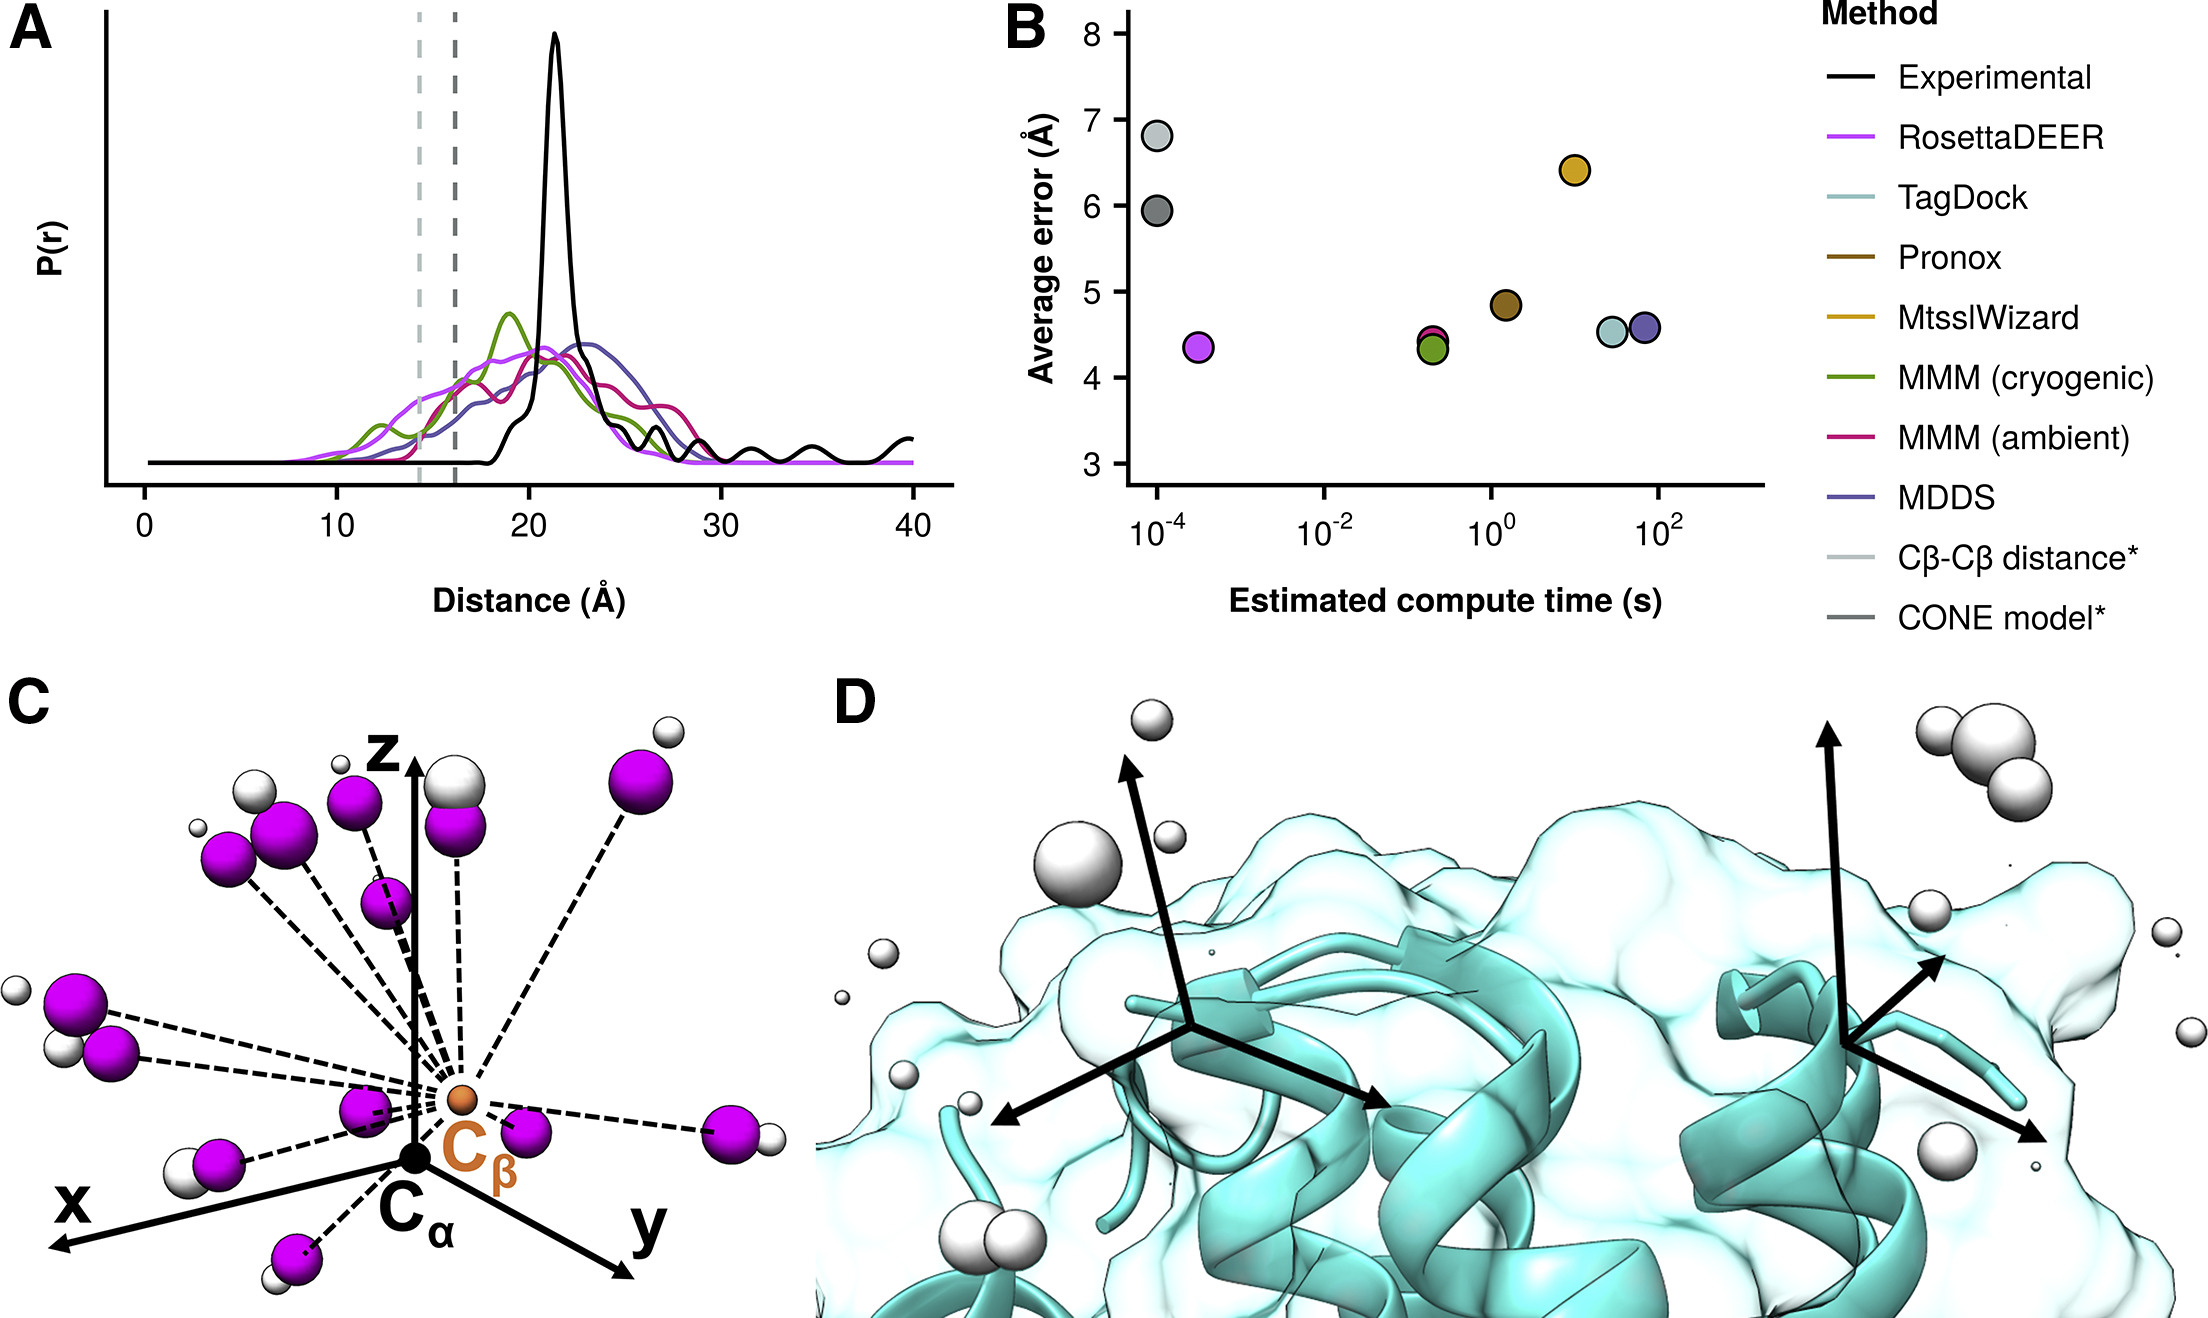
\includegraphics[width=5.5in]{rosettadeer_main_pseudorotamer.jpg}
 \caption[Simulations of distance distributions between nitroxide probes using RosettaDEER.]{Simulations of distance distributions between nitroxide probes using RosettaDEER. (A) An example of an experimentally observed distance distribution in apo Mhp1 51/278, shown in black. Distance distributions were simulated using RosettaDEER, MMM, and MDDS from the occluded Mhp1 structure (PDB: 2JLN). The average distance between $\mathrm{C_{\upbeta}}$ atoms and the average distance calculated using the CONE model shown in light gray and dark gray, respectively. (B) The estimated average time required to simulate distance distributions (*the lower limit of quantification exceeded the $\mathrm{C_{\upbeta}$-$C_{\upbeta}}$ distance compute time). (C) Coarse-grained rotameric ensemble representation of the \gls{mtssl}. Centers of mass, shown in purple, are used for clash evaluation, whereas electron coordinates, shown in gray, serve as measurement coordinates. (D) Distance distributions between residues are simulated by superimposing coordinates, evaluating clashes and measuring all resulting pairwise distances.}
\label{fig:rosettadeer_main_pseudorotamer}
\end{figure}

\subsection{RosettaDEER method description}

The Rosetta rotamer library for the paramagnetic probe \gls{mtssl} \citep*{Alexander2013} served as the basis for the coarse-grained rotameric ensemble used in this study. For each of fifty-four possible rotameric configurations, the unpaired electron was assumed to occupy the nitroxide bond midpoint; it was from these coordinates that distances would be measured. These coordinates were consolidated into a common frame defined by the $\mathrm{C_{\upalpha}}$ atom at the origin, the backbone carbonyl carbon along the Z-axis, and the backbone nitrogen in the Y-Z plane (Figure \ref{fig:rosettadeer_main_pseudorotamer}.C). The remainder of each rotamer was represented by a single pseudo-atom with a radius of \SI{2.4}{\angstrom} that was placed at 87.5\% of the distance between each nitroxide bond midpoint coordinate and an idealized $\mathrm{C_{\upbeta}}$ coordinate; if this pseudo-atom clashed with the protein model, its corresponding electron coordinate was not used for distance measurements. The placement of this pseudo-atom coincides with the center of mass of the nitroxide ring of \gls{mtssl} (all spin-labeled proteins in the PDB are listed in Table \ref{tab:rosettadeer_main_slproteins} and Figure \ref{fig:rosettadeer_supp_sl}). In cases where the steric environment prevented the placement of any coordinates, the van der Waals radius of this pseudo-atom was gradually lowered until at least one rotamer could be accommodated. Distance distributions between two residues reflect all pairwise distance measurements between their respective coordinates after evaluating clashes; we smoothed each of these distance values into gaussian distributions with a \SI{0.5}{\angstrom} standard deviation. The resulting distance distributions were then binned to \SI{0.5}{\angstrom}.

The resulting coordinate frame, which consisted of 54 unweighted coordinates and their positions with respect to protein backbone, did not account for the dynamics of the spin label (e.g. the configurations and positions it preferentially occupies) and was highly redundant, with coordinates often being placed less than \SI{1.0}{\angstrom} apart (Figure \ref{fig:rosettadeer_supp_scheme}). We addressed both issues using a scheme outlined in Figure \ref{fig:rosettadeer_supp_scheme}. Neighboring coordinates were merged using \emph{k}-means clustering to generate a series of coordinate sets ranging from 3 positions to 53 total positions. The weights of these resulting positions were then optimized using 49 previously published experimental distance distributions between 37 residues gathered in T4 Lysozyme \citep*{Islam2013}. During each of half a million iterations, a Monte Carlo Metropolis algorithm randomly modified the weight of a coordinate and either accepted or rejected the change based on the improved agreement with the experimental T4 Lysozyme distance data. This algorithm was carried out on each set of clustered coordinates one thousand times. The resulting set of weights with the best agreement consisted of seventeen coordinates, four of which were fit to be zero. This set was introduced as the default set of coordinates for RosettaDEER and was used for all subsequent experiments described here.

\subsection{Simulation of DEER dipolar coupling decay traces and comparison to experimental values}

Because the simulation of \gls{deer} decay traces has been extensively described \citep*{Hustedt2018, Jeschke2012, Jeschke2006, Marinelli2019}, here we limit our discussion to their generation from distance distributions for the purpose of evaluating protein structural models. The traces simulated by RosettaDEER ($V_{\mathup{sim}}$) are shown in Figure \ref{fig:rosettadeer_supp_alltraces} and reflect coupling between spin labels attached to the same macromolecule ($V_{\mathup{intra}}$), as well as an intermolecular “background” component reflecting coupling between spin labels across different macromolecules:

\begin{equation}\label{eq:rosettadeer_decay_complete}
V_{\mathup{sim}}\left(t_{\mathup{i}},\lambda,k,\vec{r},\vec{w}\right)=\exp\left(-k | t_{\mathup{i}} | \right)*\left(1-\lambda \left(1-V_{\mathup{intra}}\left(t_{\mathup{i}},\vec{r},\vec{w}\right)\right)\right)
\end{equation}

This background is assumed to be homogeneous across three dimensions and is modeled using a slope $k$ and a modulation depth $\lambda$. The simulated distribution consists of a vector of distances $r$ (in nanometers) and their corresponding amplitudes $w$. Simulated traces obtained this way are converted into scores ($S_{\mathup{DEER}}$) by comparing them to the corresponding experimental spectra ($V_{\mathup{exp}}$) using the following cost function:

\begin{equation}\label{eq:rosettadeer_scorefxn}
S_{\mathup{DEER}} = \frac{1}{n} \sum^{n}_{i=1} \left(V_{\mathup{exp}}\left(t_{\mathup{i}}\right)-V_{\mathup{sim}}\left(t_{\mathup{i}},\lambda,k,\vec{r},\vec{w}\right)\right)^{2}
\end{equation}

where $n$ is the number of time points in the data.

To convert a distance distribution into a spectroscopic signal that can be compared to experimental data, RosettaDEER first simulates $V_{\mathup{intra}}$ for each \SI{0.5}{\angstrom} bin $j$ between \SIrange{15}{100}{\angstrom}:

\begin{equation}
V_{\mathup{intra}}\left(t_{\mathup{i}},\vec{r},\vec{w}\right)=\sum^{m}_{j=1}w_{\mathup{j}}*\int_{0}^{\frac{\pi}{2}}\sin \theta \cos \left(\frac{\left(1-3 \cos^2 \theta\right)*\mu_{\mathup{0}} \mu_{\mathup{B}}^{2} g_{\mathup{A}} g_{\mathup{B}} t_{\mathup{i}} }{4 \pi \hslash r_{\mathup{j}}^{3}}\right) \mathup{d} \theta
\label{eq:rosettadeer_kernel}
\end{equation}

where $t$ is the time point of a trace in microseconds, $\mu_{\mathup{B}}$ is the Bohr magneton, $\mu_{\mathup{0}}$ is the vacuum permeability constant, $g_{\mathup{X}}$ is the g-factor of electron $X$, $\theta$ is the angle between the interelectron vector and the bulk magnetic field, and $m$ is the number of distance bins.

Background parameters $k$ and $\lambda$ are then determined and optimized in two stages. Initial values for both parameters were first determined by incrementing $\lambda$ with step size 0.01 and log-transforming \ref{eq:rosettadeer_decay_complete} to determine $k$ using linear regression:

\begin{equation}\label{eq:rosettadeer_logtransform}
\hat{k} = \sum^{n}_{\mathup{i}=1} \left(t_{\mathup{i}}*\ln\left(\frac{V_{\mathup{exp}}\left(t_{\mathup{i}}\right)}{1-\lambda \left(1-V_{\mathup{intra}}\left(t_{\mathup{i}},\vec{r}, \vec{w}\right)\right)}\right)\right) * \left(\sum^{\mathup{n}}_{\mathup{i}=1} t^{2}_{\mathup{i}}\right)^{-1}
\end{equation}

Subsequent attempts to fit simulated intramolecular decay traces were achieved using gradient minimization to solve for $\lambda$ and linear regression to solve for $k$. Convergence was reached when $\lvert \Delta \lambda \rvert < 0.0025$. The iterative strategy used to obtain the initial guess was repeated in cases where $\lambda$ exceeded reasonable values, the lower and upper bounds of which are defined by default as 0.02 and 0.50. This range corresponds to modulation depth values that would ordinarily be obtained from Q-band \gls{deer} on well-labeled double-cysteine mutants without using an arbitrary waveform generator. Deviations from experimentally observed values for these two parameters was found to frequently occur during the initial stages of extended chain \emph{de novo} folding, where simulated distance distributions deviated drastically from experimental values and lead to erroneous background parameter results. 

\subsection{Rosetta model generation and evaluation}\label{sec:rosettadeer_enrichment}

Rosetta models were generated with two approaches to sample a large conformational space but also ensure native-like models at a high density. The native-like models were generated with RosettaCM \citep*{Song2013} using either full-length or truncated native models as inputs. Coverage of a large conformational space was accomplished by \emph{de novo} protein folding. Bax, ExoU, and CDB3 were scored using the \emph{ref2015} energy function \citep*{Alford2017}, and Rhodopsin and Mhp1 were scored using RosettaMembrane \citep*{Yarov-Yarovoy2006}. The transmembrane regions for Rhodopsin and Mhp1 were predicted using OCTOPUS \citep*{Viklund2008}. These models were evaluated using $\mathrm{RMSD_{100SSE}}$, which measures the size-normalized \gls{rmsd} over residues in secondary structures \citep*{Carugo2002}. Enrichment of these models was evaluated as $\log_{10} \frac{TP_{\mathup{P,Score}}*N_{\mathup{Total}}}{P*N_{\mathup{Total}}}$ ⁡where $N_{\mathup{Total}}$ refers to the total number of models being considered, $P$ refers to the proportion of models considered native-like by $\mathrm{C_{\upalpha}}$ $\mathrm{RMSD_{100SSE}}$, and $TP_{\mathup{P,Score}}$ refers to the number of true positives identified in the top $P*N_{\mathup{Total}}$ models by score \citep*{Fischer2015}. We treated the top 10\% of models as native-like ($P$=0.1), thus scaling the metric from -1 (none of the top 10\% of models by $\mathrm{RMSD_{100SSE}}$ were in the top 10\% by score) to 1 (all of the top 10\% of models by $\mathrm{RMSD_{100SSE}}$ were also in the top 10\% by score), with a value of 0 indicating that the number of native-like models found in the top 10\% by score was equal to what is expected by chance.

Oscillation frequencies of decay traces in microseconds for distributions with an average distance $r_{\mathup{avg}}$ (in angstroms) were calculated as $\frac{r_{\mathup{avg}}}{5.2*10^{4}}$  \citep*{Hustedt2018}. Decay traces with fewer than three oscillations were not used to evaluate enrichment as a function of decay trace duration.

\subsection{\emph{De novo} protein structure prediction benchmark}

The protein structure prediction protocol we used largely follows a previously published template \citep*{Ovchinnikov2015} and consists of three stages. In the first stage, 10,000 models were generated using extended chain AbInitio with either RosettaDEER restraints, \gls{cone} model restraints \citep*{Alexander2008}, or no restraints. This protocol relies on the insertion of fragments obtained from a July 2011 copy of the Protein Data Bank and was obtained from the Robetta online server \citep*{Kim2004}; homologous protein structures were excluded from these fragment libraries. The contribution of the RosettaDEER score term was adjusted so that its dynamic range was similar to that of the Rosetta energy function \citep*{Ovchinnikov2015}. Since the proportion of \gls{deer} restraints relative to the protein length was comparable for Bax and ExoU, the impact of the number of restraints on the weight of the score term was not considered \citep*{Weiner2014}. 

Models generated this way were then clustered to a radius of \SI{7.5}{\angstrom} $\mathrm{C_{\upalpha}}$ $\mathrm{RMSD_{100}}$ using Durandal \citep*{Berenger2012}. Each cluster was evaluated by scoring its models using both RosettaDEER and the full-atom Rosetta energy function \citep*{Alford2017}, obtaining the cluster averages for both values, and adding their Z-scores with respect to those of other clusters. After discarding sparsely-populated clusters (smaller than 5\% of the size of the largest cluster), the top ten best-scoring models by combined Z-score were selected from the five best-scoring clusters for subsequent modeling.

An additional 1,200 models were generated from these 50 models using RosettaCM \citep*{Song2013}, which also relies on fragment insertion but ensures that the input model’s topology is retained throughout the modeling process. The scripts were obtained from a recently published refinement protocol \citep*{Park2018}, and no experimental restraints were used. Models generated during this stage were again clustered to \SI{7.5}{\angstrom} $\mathrm{C_{\upalpha}}$ $\mathrm{RMSD_{100}}$ and scored, except only the RosettaDEER score was used to evaluate the quality of these models.

During the third and final stage, models in the best-scoring cluster were minimized using FastRelax \citep*{Conway2014}, which introduces and repacks side chains while performing gradient descent on a full-atom depiction of the entire model. Models generated at this stage were scored exclusively using the native Rosetta energy function, with the lowest-scoring model selected as the output model.

\section{Results}\label{sec:rosettadeer_results}

\subsection{Modeling nitroxide spin labels using RosettaDEER}

A strategy to model proteins using \gls{deer} data must reliably simulate distance distributions between spin-labeled residues. To quantify the computational cost and efficiency of this task, we considered a panel of five proteins, listed in Table \ref{tab:rosettadeer_main_proteins}, where both atomic-detail structures and experimental \gls{deer} data were available \citep*{Altenbach2008, Bleicken2014, Fischer2017, Kazmier2014, Zhou2005}. Distance distributions between residue pairs that have been previously measured experimentally were simulated using a number of methods, and the resulting error was quantified as the difference between the average values of the simulated and experimental distance distributions (example shown in Figure \ref{fig:rosettadeer_main_pseudorotamer}.A). In addition, we measured how rapidly each program calculated these distance distributions (Figure \ref{fig:rosettadeer_main_pseudorotamer}.B). Consistent with previous results \citep*{Fischer2016, Hagelueken2012, Sale2005}, the average values of experimental distance distributions gathered in monomeric proteins, but not the homodimer CDB3, agree more closely with those of simulated distributions than their corresponding $\mathrm{C_{\upbeta}}$-$\mathrm{C_{\upbeta}}$ distances, from which restraints such as the \gls{cone} model are derived \citep*{Alexander2008}. By contrast, none of the methods examined here reliably reproduced the width of the distance distributions. This is likely attributable to oversampling of available conformational space of the spin label, which results from the exclusive use of van der Waals repulsive energies to limit possible rotameric configurations. Finally, the data revealed how simulation times varied substantially between these methods.

These results further illustrate that increasing computational complexity did not lead to more accurate distance distributions. We hypothesized that, for the same reason, decreasing the computational complexity would not lead to less accurate distance distributions. Therefore, RosettaDEER’s design prioritized computational efficiency (see section \ref{sec:rosettadeer_methods}). Rather than measure distances from full-atom rotamers or mobile dummy atoms, RosettaDEER uses a probability density function to capture high-occupancy electron positions that would be explored by \gls{mtssl} and map them onto the protein structure (Figures \ref{fig:rosettadeer_main_pseudorotamer}.C and D). For each of these coordinates, an evaluation of a potential van der Waals overlap was performed between a pseudo-atom representing the nitroxide ring’s center of mass and the rest of the protein. Placing this pseudo-atom at an idealized location, consistent with spin-labeled protein structures in the Protein Databank (Figures \ref{fig:rosettadeer_supp_sl} and Table \ref{tab:rosettadeer_main_slproteins}), reduced the number of atoms for this evaluation to one per rotamer, thus maximizing computational efficiency. Figures \ref{fig:rosettadeer_main_pseudorotamer}.A and B demonstrate that RosettaDEER’s simplified representation of the spin label allows the generation of distance distributions three to five orders of magnitude faster than other approaches but with comparable accuracy.

\begin{figure}[h!]
\centering
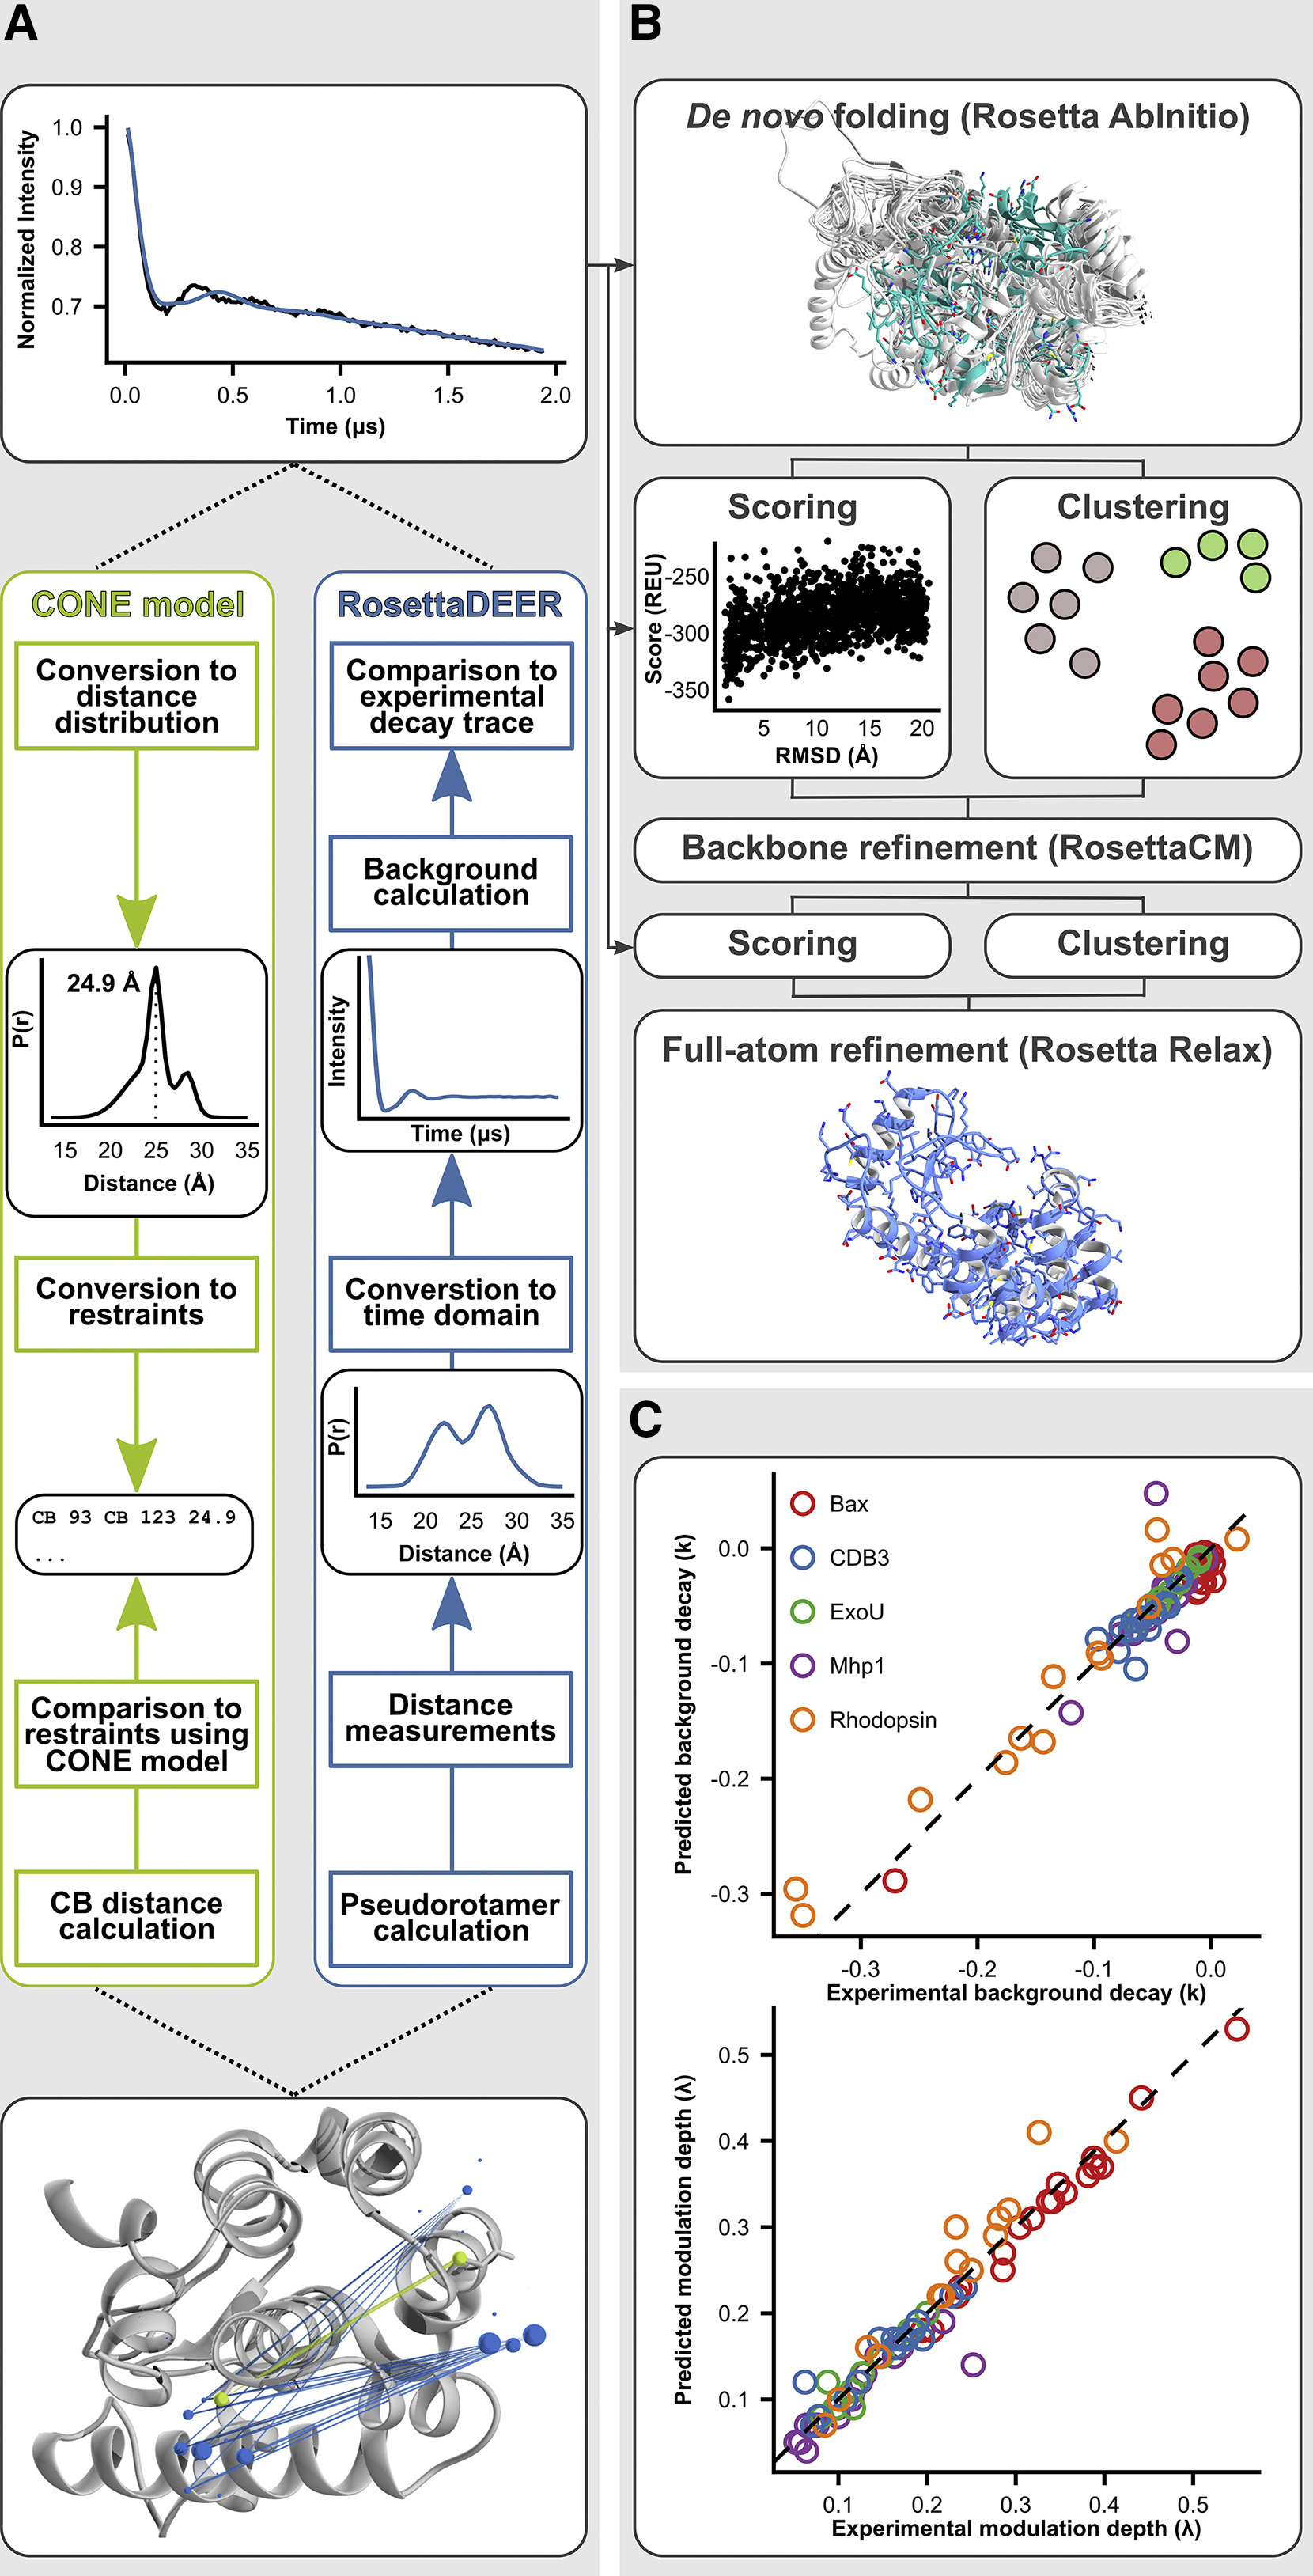
\includegraphics[width=3.25in]{rosettadeer_main_scheme.jpg}
 \caption[RosettaDEER simulations of distance distributions and decay traces.]{RosettaDEER simulations of distance distributions and decay traces. The forward approach taken by RosettaDEER contrasts with the preprocessing required by the CONE model. (A) A flowchart illustrating how both the CONE model and RosettaDEER use experimental \gls{deer} data to model proteins (example shown is T4 lysozyme residues 93 and 123). (B) Incorporation of \gls{deer} experimental restraints into Rosetta structure prediction pipeline. (C) Recovery of experimental background coupling and modulation depth parameter values.}
\label{fig:rosettadeer_main_scheme}
\end{figure}

\subsection{Comparison of simulated with experimental DEER decay traces}

Most existing methods that leverage \gls{deer} experimental data for structural modeling require the primary spectroscopic readout first be processed into a distance distribution. A conventional approach, such as the Rosetta \gls{cone} model, is outlined in Figure \ref{fig:rosettadeer_main_scheme}.A. This involves 1) manually identifying and removing the “background” signal, which corresponds to coupling between spin labels across macromolecules; 2) using Tikhonov regularization to convert the remaining intramolecular signal into a distance distribution; and 3) selecting a single distance value from this distribution to restrain the modeling process. An additional bias is often required to convert these distance data into backbone restraints \citep*{Alexander2008, Alexander2013, Sale2004, Yang2010}.

We reasoned that these preprocessing steps could be avoided by simulating a spectroscopic signal from candidate models for direct comparison to the experimental data. As with other forward approaches to fitting \gls{deer} data \citep*{Hustedt2018, Stein2015}, the steps are as follows: 1) the model is used to generate a distance distribution; 2) this distance distribution is converted into a spectroscopic signal consisting solely of the effect of coupling between spin labels attached to the same macromolecule; and 3) the slope of the “background” coupling and depth of modulation needed to optimally fit the simulated and experimental decay traces is determined.

This final step represents the outstanding challenge in the proposed pipeline, as most modeling programs, including Rosetta, focus on isolated protein structural models. We instead used a two-parameter exponential function to simulate the background coupling ($k$) and modulation depth ($\lambda$) (see Section \ref{sec:rosettadeer_methods}). The values of these parameters were determined by minimizing the sum of the squared residuals. The optimum values obtained strongly correlated with those obtained using DeerAnalysis \citep*{Jeschke2006}, with $r^2$ values exceeding 0.90 for both parameters (Figure \ref{fig:rosettadeer_main_scheme}.C), despite the fact that the inaccuracies in the distance distributions affected the fit (Figure \ref{fig:rosettadeer_supp_alltraces}). In fact, we found that this correspondence correlated less strongly with the goodness-of-fit in the distance domain than it did with the quality of the experimental data in the time domain (Figure \ref{fig:rosettadeer_supp_oscillations}).

\subsection{Enrichment of native-like models using experimental decay traces}

Being able to simulate \gls{deer} traces from candidate structural models without any pre-processing offers the possibility to reframe the problem currently faced by translating the \gls{deer} traces into distance distributions. Whereas methods such as Tikhonov regularization convert individual \gls{deer} traces into distance distributions, RosettaDEER, in conjunction with Monte Carlo modeling, would instead seek to determine the structural model most consistent with both an energy function and the experimental data. To investigate whether unprocessed \gls{deer} traces can be used to discriminate native-like models from incorrectly-folded models, we generated a series of 1000-2000 misfolded models for each of the five proteins in our test set and scored their agreement with experimental \gls{deer} data. In addition, we generated 1000 docked models of the homodimer CDB3 that retained the native fold for the protomer, but not the oligomeric interface. Similarity to the native model was measured by $\mathrm{C_{\upalpha}}$ $\mathrm{RMSD_{100SSE}}$ \citep*{Carugo2002}, which is the size-normalized root means squared deviation across secondary structural elements (Figure \ref{fig:rosettadeer_main_zscores}). RosettaDEER’s effectiveness at this task was measured by the enrichment parameter, which is defined in the Section \ref{sec:rosettadeer_enrichment} section and quantifies a scoring function’s ability to discriminate native-like models from incorrectly-folded models.

\begin{wrapfigure}{ro!}{0.55\textwidth}
    \centering
    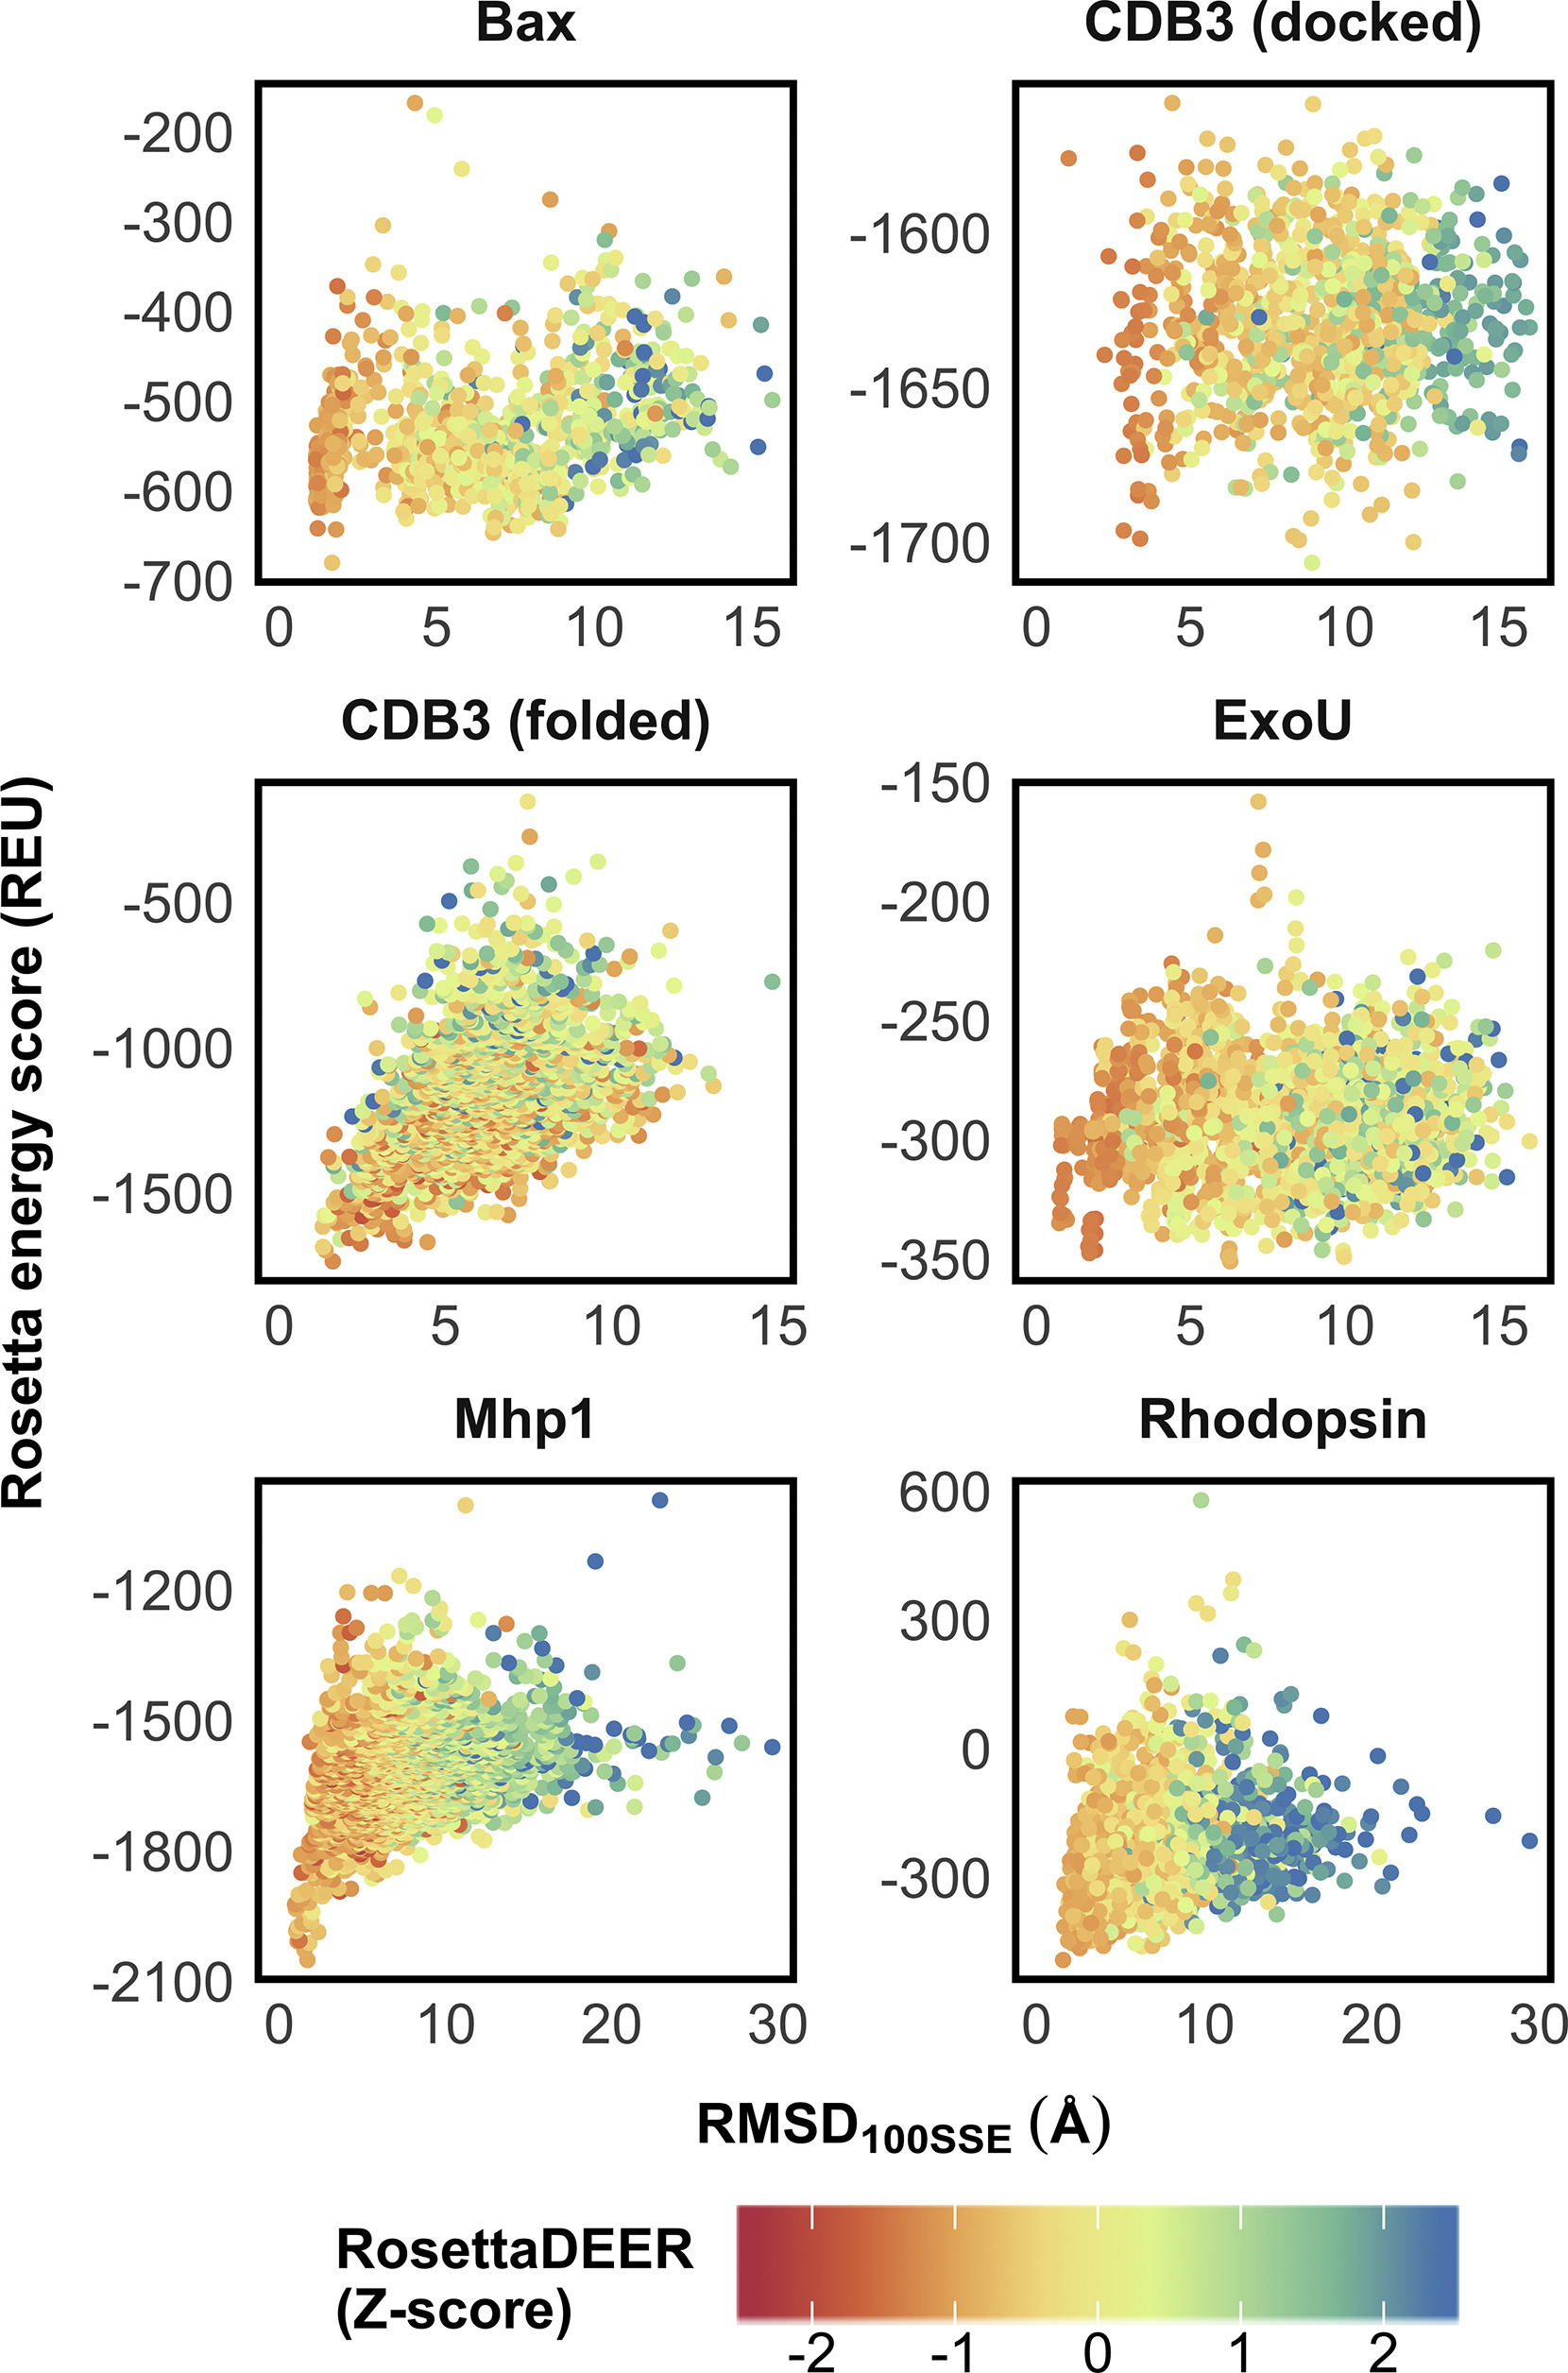
\includegraphics[width=3.25in]{Figures/rosettadeer_main_zscores.jpg}
     \caption[Evaluation of models using \gls{deer} decay traces.]{Evaluation of models using \gls{deer} decay traces. Models with $\mathrm{C_{\upalpha}}$ $\mathrm{RMSD_{100SSE}}$ ranging from \SI{0.5}{\angstrom} to \SI{30.0}{\angstrom} were scored using both the Rosetta energy function and RosettaDEER.}
    \label{fig:rosettadeer_main_zscores}
\end{wrapfigure}

RosettaDEER consistently scored native-like models of the monomeric proteins more favorably than poorly-folded models (Figure \ref{fig:rosettadeer_main_zscores}). This was also observed with correctly-docked models of CDB3. Moreover, it generally outperformed the \gls{cone} model in enriching native-like models (Figure \ref{fig:rosettadeer_supp_oscillation_decoys}). Perhaps unsurprisingly, the simultaneous use of Rosetta’s energy function often improved enrichment, since it overwhelmingly considers short-range interactions and is therefore expected to complement the evaluation of longer ranger, fold-level information provided by \gls{deer} restraints (Figure \ref{fig:rosettadeer_supp_oscillation_decoys}) \citep*{Alford2017}. We note that RosettaDEER could not effectively identify misfolded models of CDB3, which we attribute to the fact that \gls{deer} restraints reflect distances across the center of symmetry, rather than within the protomer. Nevertheless, these results suggest that RosettaDEER’s inability to perfectly recreate the experimental \gls{deer} data did not impede its ability to identify correctly folded models, suggesting that it could be effectively used for structure prediction.



The fact that structural models are scored based on their consistency with the primary spectroscopic data led us to hypothesize that they could be evaluated using lower-quality data than what would be necessary for conversion into precise distance distributions. We were specifically interested in evaluating the importance of the experimental data’s time window, which must undergo roughly 0.8 and 1.6 oscillations for Tikhonov regularization to accurately identify a distance distribution’s average and standard deviation, respectively \citep*{Jeschke2012}. This hypothesis was tested by artificially truncating the experimental data in the time domain and measuring enrichment as a function of how many oscillations were included (see \ref{sec:rosettadeer_methods} and Figure \ref{fig:rosettadeer_supp_oscillation_decoys}). Strikingly, RosettaDEER could enrich native-like models of Bax, ExoU, Rhodopsin, and Mhp1 with highly truncated data ($\mathrm{<0.8}$ oscillations), albeit to a reduced degree. We found that the addition of data in the time domain beyond one oscillation failed to lead to any measurable improvements in enrichment, despite its importance in allowing RosettaDEER to identify the correct background coupling parameters (Figure \ref{fig:rosettadeer_supp_oscillations}). These results suggest that RosettaDEER is more permissive than Tikhonov regularization with respect to the effect of data quality on protein structural modeling.

\subsection{\emph{De novo} folding of Bax and ExoU}\label{sec:rosettadeer_folding_results}

To further illustrate RosettaDEER’s capability to identify native-like models, we folded Bax and ExoU \emph{de novo} using experimental \gls{deer} decay data. These two proteins were chosen because native-like models cannot be identified using the default Rosetta energy function alone (Figures \ref{fig:rosettadeer_main_zscores} and \ref{fig:rosettadeer_supp_oscillation_decoys}). The structure prediction protocol we used is similar to one used to model proteins using other types of sparse data \citep*{Kim2004, Ovchinnikov2015} and is illustrated in Figure \ref{fig:rosettadeer_main_scheme}.B and described in detail in \ref{sec:rosettadeer_methods}. We first generated an initial set of ten thousand models using Rosetta AbInitio folding supplemented by either experimental restraints through RosettaDEER, experimental restraints through the \gls{cone} model \citep*{Alexander2008}, or no restraints. These models were then clustered, and models from the best-scoring clusters were refined and recombined into one thousand two hundred new models without using experimental data. After a second round of clustering, models from the cluster with the best agreement to the experimental data were refined and minimized, and the model with the best Rosetta energy score was returned as the predicted model. 

\begin{wrapfigure}{l}{0.55\textwidth}
    \centering
    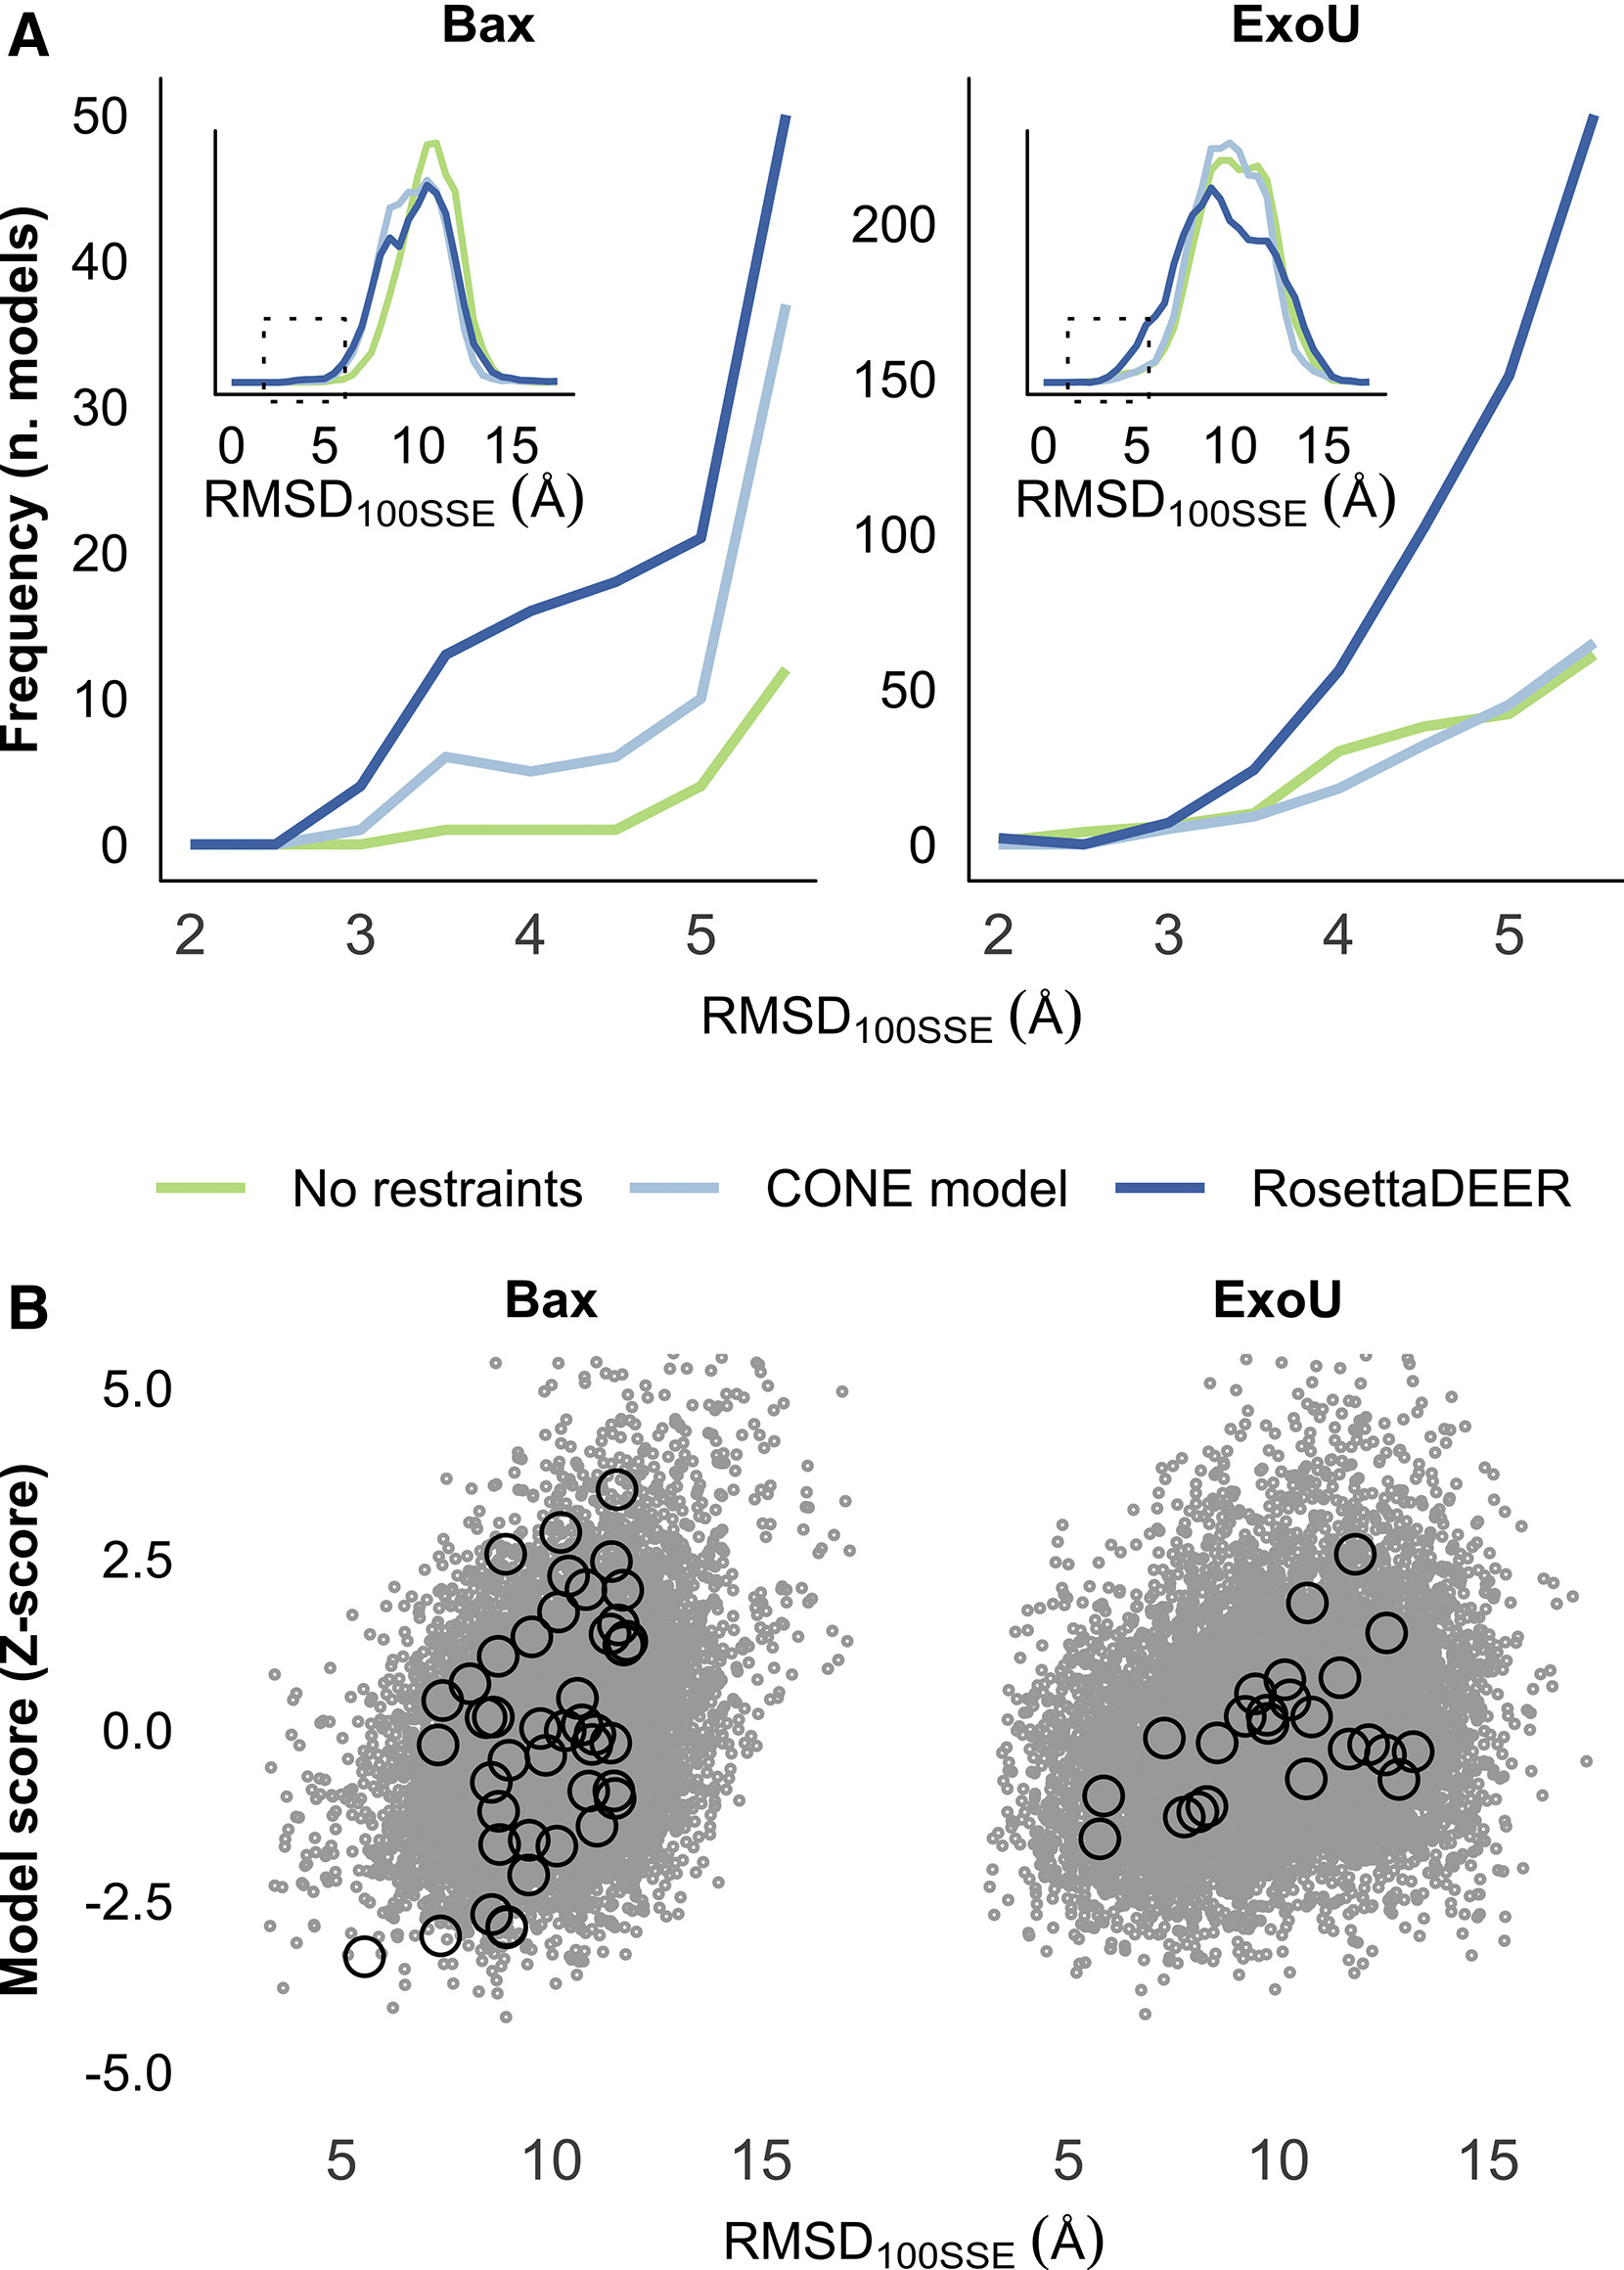
\includegraphics[width=3.25in]{Figures/rosettadeer_main_folding.jpg}
     \caption[Structure prediction of Bax and ExoU using experimental decay data.]{Structure prediction of Bax and ExoU using experimental decay data. (A) \emph{De novo} protein folding of native-like models using \gls{deer} decay restraints with RosettaDEER, $\mathrm{C_{\upbeta}}-\mathrm{C_{\upbeta}}$ distance restraints with the CONE model, or no restraints. Inset: spread of all models generated using these three methods. (B) Accuracy of \emph{de novo} folded models (gray dots) and clusters (black circles) as a function of combined \gls{deer} and Rosetta Z-score.}
    \label{fig:rosettadeer_main_folding}
\end{wrapfigure}

In the absence of experimental restraints, few of the models generated by AbInitio folding resembled the native fold (Figure \ref{fig:rosettadeer_main_folding}.A). Perhaps strikingly, providing \gls{deer} restraints with the \gls{cone} model had no effect on the proportion of native-like models of ExoU generated this way (a measurable improvement was observed when folding Bax). This contrasts with the proportion of native-like models generated using RosettaDEER, which was substantially higher in the case of both proteins.

Although agreement between models and experimental structures loosely correlated with both RosettaDEER score and Rosetta energy score for both proteins, an abundance of incorrectly-folded models obscured this trend (Figure \ref{fig:rosettadeer_main_folding}.B; RosettaDEER and Rosetta energy scores were jointly considered by adding the Z-scores of each). As a result, we were unable to identify native-like models for either Bax of ExoU from score values alone. The ten best-scoring models by these metrics were generally incorrectly folded (\SIrange{5}{10}{\angstrom} $\mathrm{C_{\upalpha}}$ $\mathrm{RMSD_{100SSE}}$) and buried amphipathic features found on the surface of the native model. This shortcoming is typically addressed by clustering, since native-like models are more likely to be found near the centers of large clusters with favorable average scores \citep*{Shortle1998}. We therefore clustered Bax and ExoU models with a radius of \SI{7.5}{\angstrom} and evaluated these clusters by taking the Z-scores of both the average Rosetta energy and RosettaDEER score and adding them together (Figure \ref{fig:rosettadeer_main_folding}.B). In the case of both proteins, this step placed native-like models in the best-scoring clusters. Focusing our attention on the five best-scoring clusters allowed us to discard 85.3\% of the Bax models and 61.3\% of the ExoU models, while retaining a majority of the native-like models in each case.

\begin{wrapfigure}{R}{0.6\textwidth}
    \centering
    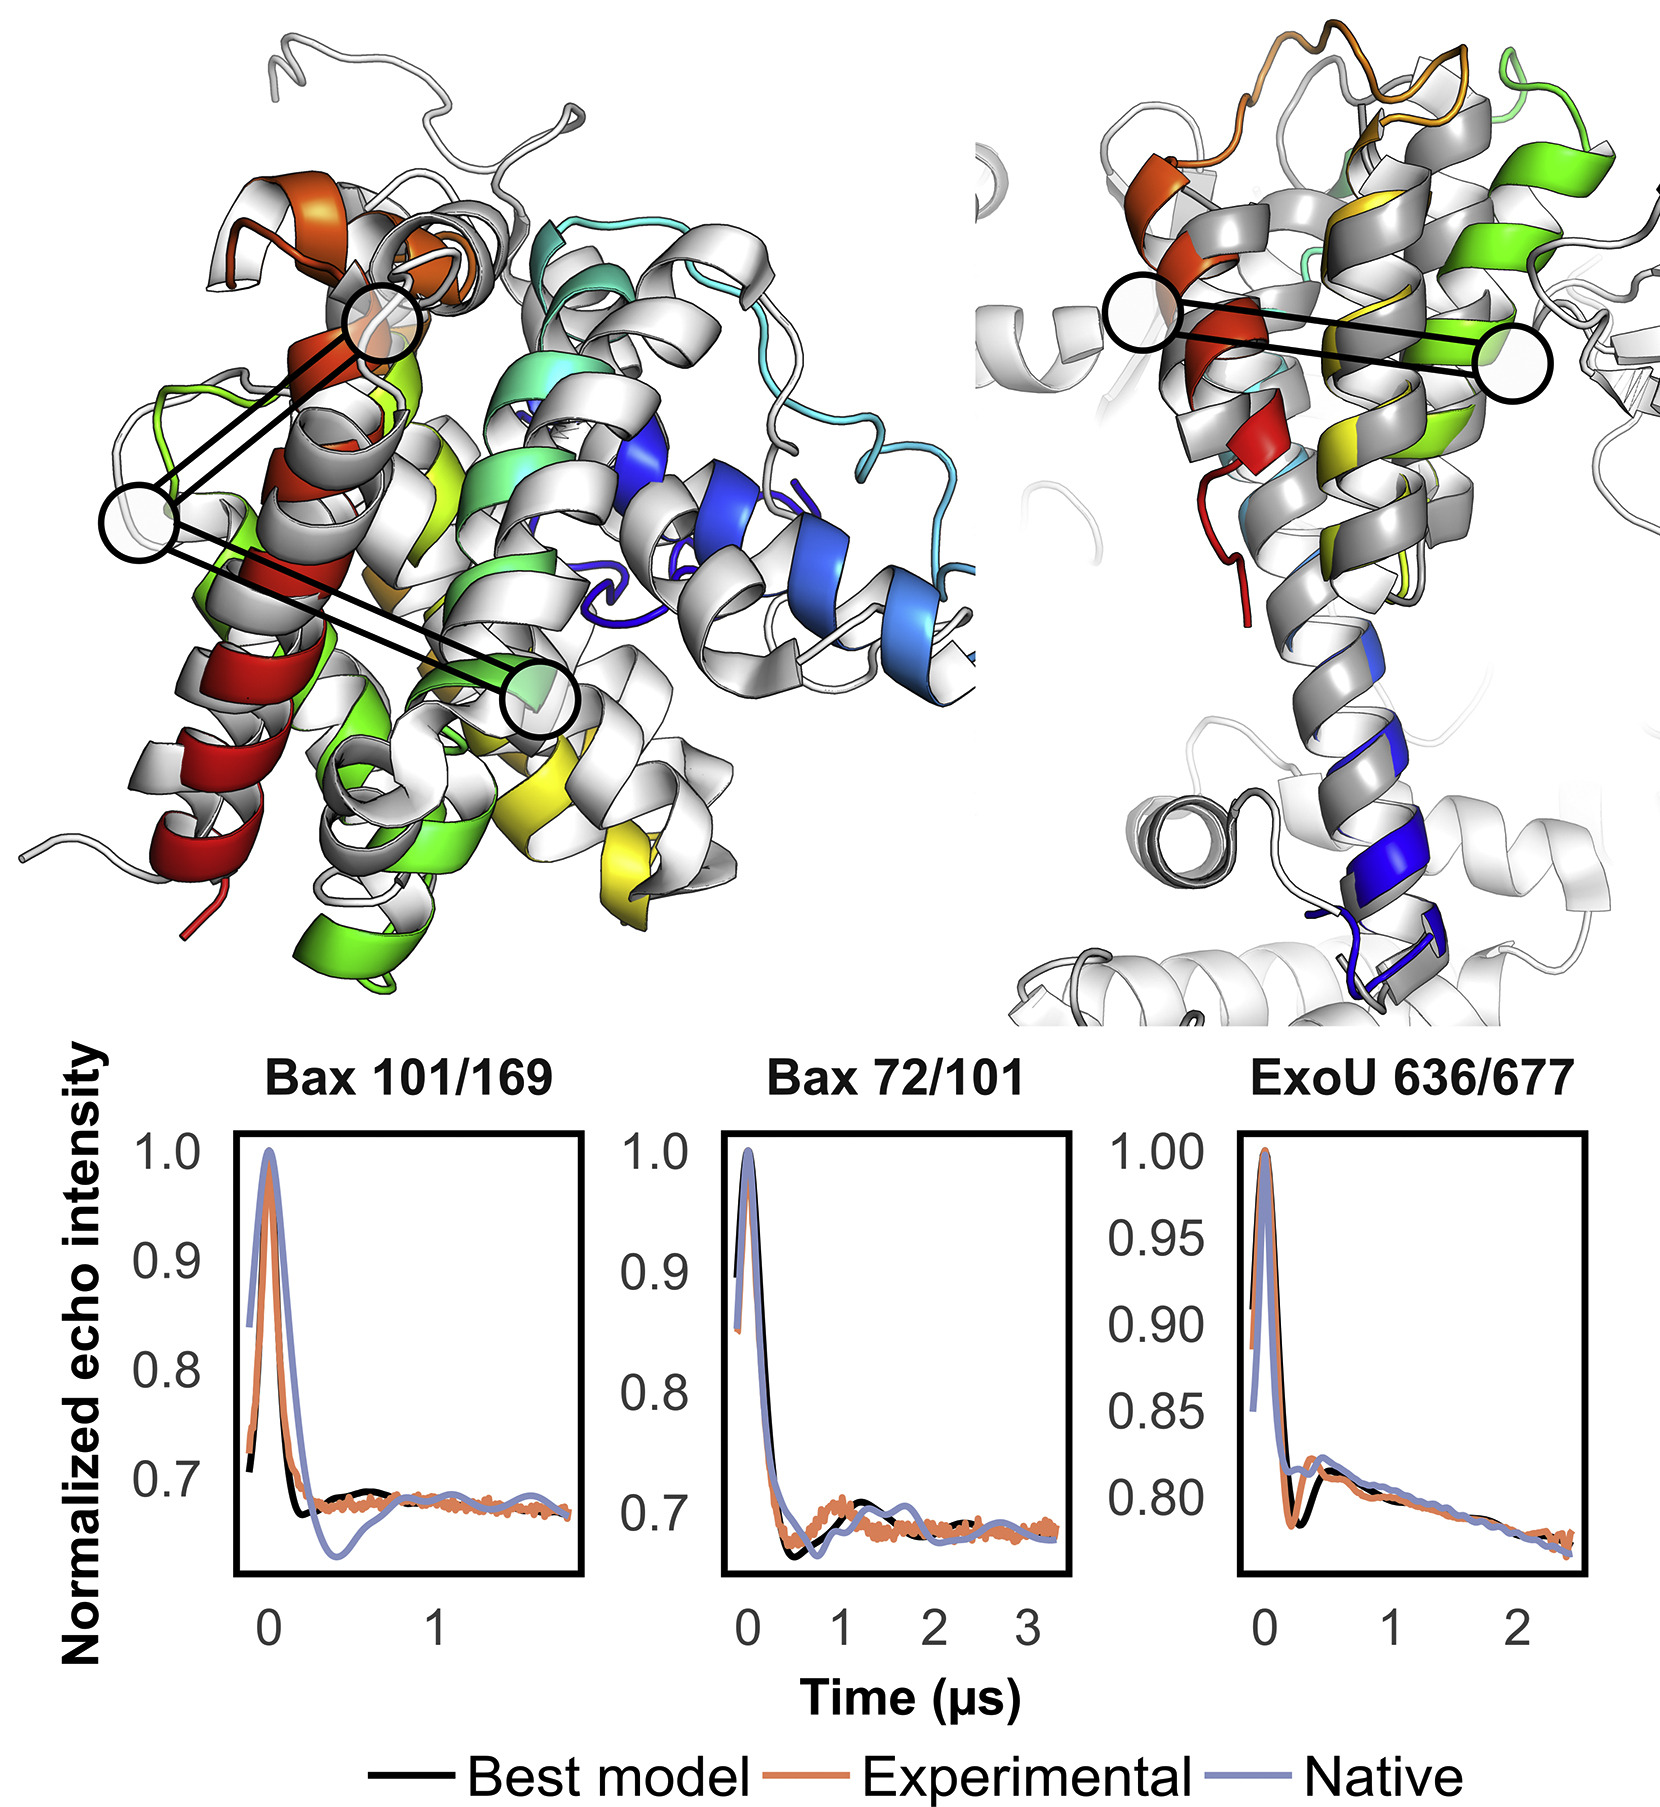
\includegraphics[width=3.25in]{Figures/rosettadeer_main_bestmodels.jpg}
     \caption[Predicted models of Bax and ExoU generated using DEER data.]{Predicted models of Bax and ExoU generated using DEER data. Best-scoring models of Bax and ExoU had an accuracy of \SI{3.2}{\angstrom} and \SI{2.1}{\angstrom} $\mathrm{C_{\upalpha}}$ $\mathrm{RMSD_{100SSE}}$, respectively.(Top) Models were obtained from 10,000 \emph{de novo} folded models, the best-scoring of which were refined into 1200 additional models. Native models shown in white. (Bottom) Example \gls{deer} traces in which the best model outperformed the native. Corresponding residues indicated as circles in (A) and (B).}
    \label{fig:rosettadeer_main_bestmodels}
\end{wrapfigure}

Each cluster at this stage represented a broad population of models that satisfied the \gls{deer} data. To test whether refining models without experimental restraints would reveal the native fold, ten models from each of the top five clusters were refined and recombined using RosettaCM \citep*{Song2013}. This step retained the topology of the input models, but permitted minor backbone rearrangements that allowed misfolded models to optimize away from conformations consistent with the experimental data. As a result, the cluster with the most native-like models after this resampling stage scored the most favorably by RosettaDEER. After minimization of models in this cluster \citep*{Conway2014}, the best-scoring model by Rosetta score for both Bax and ExoU had near-native folds (<\SI{3.5}{\angstrom} $\mathrm{C_{\upalpha}}$ $\mathrm{RMSD_{100SSE}}$; Figure \ref{fig:rosettadeer_main_bestmodels} and \ref{fig:rosettadeer_supp_top3}).

\section{Discussion}

RosettaDEER predicts and refines protein structures by integrating \gls{deer} spectroscopy data and Rosetta computational modeling protocols. The novel aspects of this method are a simplified representation of the commonly used spin label \gls{mtssl} and a strategy to rapidly simulate \gls{deer} decay traces for comparison to uncorrected experimental traces. The robustness of the method was demonstrated by benchmarking every step on five sparse datasets. Despite the simplified spin label representation, the distance distributions simulated by RosettaDEER are comparable to those generated using more computationally complex rotamer library approaches. Moreover, even though simulated spectra fail to perfectly fit experimental \gls{deer} traces, this integrated approach efficiently identifies conformations that simultaneously satisfy the data and the Rosetta energy function. Our findings illustrate how RosettaDEER can complement similar methods that are more computationally intensive but able to use \gls{deer} decay data to perform high-resolution refinement of protein structures \citep*{Marinelli2019}.

The \emph{de novo} folding benchmark with the small soluble proteins ExoU and Bax highlights the success of this strategy. Both proteins possess surface-exposed amphipathic regions that insert into the membrane. Bax transitions from a soluble monomer into a membrane-bound oligomer using its C-terminal helix \citep*{Bleicken2014}, whereas ExoU is hypothesized to move into the membrane using a flexible loop between its two C-terminal helices \citep*{Tessmer2017}. Consistent with previous results \citep*{Fischer2017, Fischer2016}, the Rosetta energy function favored models that packed these substructures in the protein core, leading to incorrectly folded models and lack of correlation between the Rosetta score and model accuracy. As a result, orthogonal experimental data that define the structure are critical to \emph{de novo} folding. Our folding benchmark suggests that RosettaDEER more effectively leverages the experimental data than the $\mathrm{C_{\upbeta}}$-based \gls{cone} model. Moreover, even low-quality data can be used to discriminate native-like from incorrectly-folded models. We appreciate that, for larger proteins, structure determination from \gls{deer} experiments alone would require extensive experimental data. Integrating RosettaDEER with other types of sparse experimental data could therefore reduce the number of \gls{deer} restraints required for accurate modeling.

The strategy of RosettaDEER to predict the structures of these two proteins leverages the experimental data by folding and optimizing protein structures with and without restraints, respectively. The first step leads to a substantial reduction in the search space and a concomitant increase in the number of models that satisfy the restraints, although not all of these models are correctly folded. After clustering the models to remove those that correspond to narrow energy minima, the second step, optimization without restraints, allows clusters with incorrectly folded models to reach energy minima inconsistent with the data. This filtering procedure restores the experimental data’s ability to identify native-like models, since the most native-like models of Bax and ExoU at this stage were not identifiable using the Rosetta energy function. Overall, this protocol decreases both the number of incorrectly-folded structures that fit the data and the conformational search space inherent to the protein folding problem.

Despite its success illustrated here, the current implementation of RosettaDEER assumes that a single protein conformation describes the data. For example, the distance distributions of Mhp1, the most conformationally flexible protein examined in this dataset, were generally more poorly simulated using available methods than those collected in other proteins. Experimental applications of the \gls{deer} technique often focus on monitoring ensembles of protein conformations. They can therefore be effectively complemented by computational methods that interpret this data with the capability to generate multiple models and examine their consistency with sparse experimental data.

\section{Acknowledgements}

The authors would like to thank Dr. Christian Altenbach, Dr. Enrica Bordignon, and Dr. Eric Hustedt for providing experimental data used in this study and Dr. Rocco Moretti, Dr. Axel Fischer, and Dr. Andrew Leaver-Fay for helpful discussions on designing and implementing RosettaDEER. Research was funded by the National Institutes of Health (R01 GM080403, R01 GM073151, R01 GM114234, R01 GM077659, R01 HL122010, and R01 HL144131).
\clearpage % clear the prior chapter's page

\chapter{Methodology for rigorous modeling of protein conformational changes by Rosetta using DEER distance restraints}\label{ch:multilateration}
%\vspace{-7mm}
%\bigskip

The contents of this chapter have been previously published \citep*{DelAlamo2021a}.

\bigskip

We describe an approach for integrating distance restraints from \gls{deer} spectroscopy into Rosetta with the purpose of modeling alternative protein conformations from an initial experimental structure. Fundamental to this approach is a multilateration algorithm that harnesses sets of interconnected spin label pairs to identify optimal rotamer ensembles at each residue that fit the \gls{deer} decay in the time domain. Benchmarked relative to data analysis packages, the algorithm yields comparable distance distributions with the advantage that fitting the \gls{deer} decay and rotamer ensemble optimization are coupled. We demonstrate this approach by modeling the protonation-dependent transition of the multidrug transporter PfMATE to an inward facing conformation with a deviation to the experimental structure of less than \SI{2}{\angstrom} $\mathrm{C_{\upalpha}}$ \gls{rmsd}. By decreasing spin label rotamer entropy, this approach engenders more accurate Rosetta models that are also more closely clustered, thus setting the stage for more robust modeling of protein conformational changes.

\section{Introduction}\label{sec:multilateration_main_intro}

Distance measurements between pairs of spin labels by \gls{deer} spectroscopy have been utilized extensively to investigate the structures and dynamics of proteins \citep*{Collauto2017, Evans2020, Kazmier2014, Mishra2014} and the assembly of protein-protein complexes \citep*{Bhatnagar2007, Kim2018, Kim2011, Tessmer2018}. At the fundamental level, \gls{deer} measures magnetic dipolar coupling to infer the distributions of distances between two or more spin labels \citep*{Jeschke2012, Mchaourab2011}. A two-step process typically interprets these distances as spatial restraints describing the protein backbone structure. First, the echo-decay time traces are transformed into distributions consisting of distance components characterized by a mean and width \citep*{FabregasIbanez2020, Hustedt2018, Jeschke2004, Pannier2000, Stein2015}. Second, these distributions are compared to those predicted using one of several strategies, ranging from generic rotamer libraries\citep*{Hagelueken2012, Polyhach2011, Reichel2018}, explicitly modeled pseudoatoms\citep*{Kazmier2014, Raghuraman2014}, or explicitly modeled spin label side chains \citep*{Alexander2013, Dastvan2016, Krug2016, Marinelli2019, Sale2005, Spicher2020}. However, these strategies tend to overestimate the dynamics of flexible probes such as the commonly used \gls{mtssl}. Therefore, the predicted distributions are broad relative to the experimental ones \citep*{Hagelueken2012, Hatmal2012, Islam2013, Jeschke2013, Klose2012}, which hinders \gls{deer}-based evaluation of protein structures or complexes as well as mapping of protein conformational changes. The latter can be obscured entirely if modeled distribution widths exceed distance changes observed between spin labels.1 Another layer of complications in modeling of conformational changes arises if the ensemble of spin label rotamers is allowed to reconfigure, hence providing a low energy pathway to account for changes in distance distributions that originate from backbone movements. Collectively, these caveats limit the accuracy and precision of molecular models generated from \gls{deer} restraints.

Several algorithms have recently been developed to refine ensembles of spin label rotamers by employing multilateration \citep*{Abdullin2015, Gaffney2012, Hagelueken2013, Hays2019, Jeschke2018, Reichel2018}. Multilateration refers to the determination of an object’s position in three-dimensional space given its distance from a constellation of points; common applications include the positioning of electronic devices using the Global Positioning System and of earthquakes epicenters using time-of-arrival data \citep*{Fang1986}.  To utilize this approach to position spin label rotamers requires both a high-resolution starting structure and a set of \gls{deer} distance data consistent with that structure. However, a unique challenge in this endeavor is that spin labels are flexible relative to the protein backbone.  As a result, the ensembles characterizing their positions must be refined simultaneously for all spin labels in a given protein model. 

Molecular dynamics simulations have been used to determine a set of optimized rotamers from explicitly modeled spin labels restrained by experimental distance distributions \citep*{Hustedt2018, Marinelli2015, Marinelli2019, Roux2013}. Alternatively, rotamer libraries have been precomputed and reweighed using either Monte Carlo \citep*{Gaffney2012, Hays2019}, singular value decomposition \citep*{Hagelueken2013}, or nonlinear least-squares minimization \citep*{Jeschke2018}. The positions of these labels can, in turn, be used to more precisely locate paramagnetic ligands or metal ions \citep*{Abdullin2015, Abdullin2021, Gaffney2012, Yang2012} as well as make small-scale refinements to protein structures \citep*{Reichel2018, Wingler2019}. To our knowledge, however, none of these methods have demonstrated that these optimized rotamers can lead to improvements in modeling conformational changes.

Furthermore, these methods generally do not address unique factors confounding multilateration of spin labels. First, the width of a distribution reflects disorder in the solid state as a result of backbone and spin label side chain dynamics at room temperature. Existing multilateration methods generally ignore the former, by assuming the distribution is explained entirely by spin label dynamics \citep*{Gaffney2012, Reichel2018}, or both, by extracting the peak distance from the distribution and discarding the width \citep*{Wingler2019}. Second, relying on distance distributions rather than time domain data propagates assumptions intrinsic to the method used for the transformation of the latter. Depending on the noise level of the experimental measurements, this step can distort true components or introduce ghost components to the distribution. Finally, although \gls{deer} distributions are often reported with confidence bands to reflect the uncertainty inherent to this transformation \citep*{Edwards2016, FabregasIbanez2020, Hustedt2018}, they are generally taken at face value when used for rotamer multilateration. This incorrectly implies that experimental uncertainty is uniformly distributed across the dataset and can lead to rotamers that over- or underfit the \gls{deer} distributions. Collectively, these obstacles prevent the straightforward positioning of spin label ensembles in three-dimensional space and complicate the confidence with which such ensembles can be used for subsequent modeling purposes.

To address these issues, we developed and implemented, as part of the RosettaDEER module, an algorithm that combines rotamer multilateration \citep*{Abdullin2021, Gaffney2012, Jeschke2018} for pairs sharing common spin labeling sites with direct analysis of \gls{deer} time traces. The algorithm calculates a weighted distribution of “pseudo-rotamers”, or inflexible coarse-grained side chains, capable of recapitulating large experimental datasets collected using \gls{deer}. Importantly, this algorithm goes beyond comparable methods by refining these ensembles using raw data in the time domain, rather than distance distributions calculated \emph{a priori}, thus avoiding the loss of information that can occur as result of data transformation. Using experimental collected in the model system T4 Lysozyme and the multidrug transporter PfMATE, we demonstrate that this algorithm is able to fit time domain data as effectively as widely-used \gls{deer} data analysis programs. Integrated with Rosetta, these rotamers ensembles yield substantial improvements in both accuracy and precision of modeling the outward-to-inward isomerization of the multidrug transporter PfMATE, thus reinforcing the notion that coupling analysis of primary data with rotamer optimization is a superior approach for restrained modeling of protein conformational states. 

\section{Results and Discussion}

\subsection{Overview of the multilateration algorithm}

The algorithm capitalizes on the concept of pseudo-rotamers, which are simplified representations of the spin label designed to maximize computational efficiency. A pseudo-rotamer models the spin label side chain as a centroid atom representing the nitroxide ring and its unpaired electron, yielding predicted distance distributions that are comparable to full-atom depictions. Unlike explicit depictions of the spin label used in all-atom simulations, ensembles of pseudo-rotamers do not interact with one another; as a result, the dynamics of spin labels close in space are fully independent. However, in principle, any rotamer library can be used for the multilateration strategy described here \citep*{Alexander2013, Fajer2015, Hagelueken2012, Hatmal2012, Polyhach2011, Spicher2020}.

The transformation of DEER data to distance distributions is an ill-posed mathematical problem necessitating the use of either regularization \citep*{Chiang2005, FabregasIbanez2020, Jeschke2006}, parametric modeling \citep*{FabregasIbanez2020, Hustedt2018, Stein2015}, neural networks \citep*{Worswick2018}, or other methods \citep*{Edwards2016, Pannier2000, Srivastava2016}. Because these methods have intrinsic approximations which could interfere with rotamer ensemble determination, we elected to fit the raw experimental data directly using an iterative simulated annealing strategy that 1) measures all pairwise distances between pseudo-rotamers, 2) converts each distance distribution into a \gls{deer} decay, and 3) calculates the intermolecular dipolar coupling contribution by nonlinear least-squares minimization (Figure \ref{fig:multilateration_main_scheme}). Different levels of noise between \gls{deer} traces linked by multilateration were normalized using estimates obtained from each signal’s corresponding imaginary component \citep*{Marinelli2019}. The algorithm prioritized the generation of parsimonious ensembles by minimizing the total number of pseudo-rotamers with nonzero weights using the \gls{aicc} \citep*{Akaike1973, Sugiura1978}. This metric, which allows for regularization in rotamer space rather than the distance domain, was guided by the heuristic that the flash-freezing process sharpens the distribution of rotamers that contribute to the \gls{deer} signal \citep*{Banham2007, Georgieva2012}. Finally, to account for backbone heterogeneity and the expectation of smoothness in the distance domain, simulated distributions were broadened by a magnitude corresponding to the residues’ intrinsic flexibility, as reported by their respective crystallographic B-factor values \citep*{Sun2019, Yang2007}.

\begin{figure}[h!]
\centering
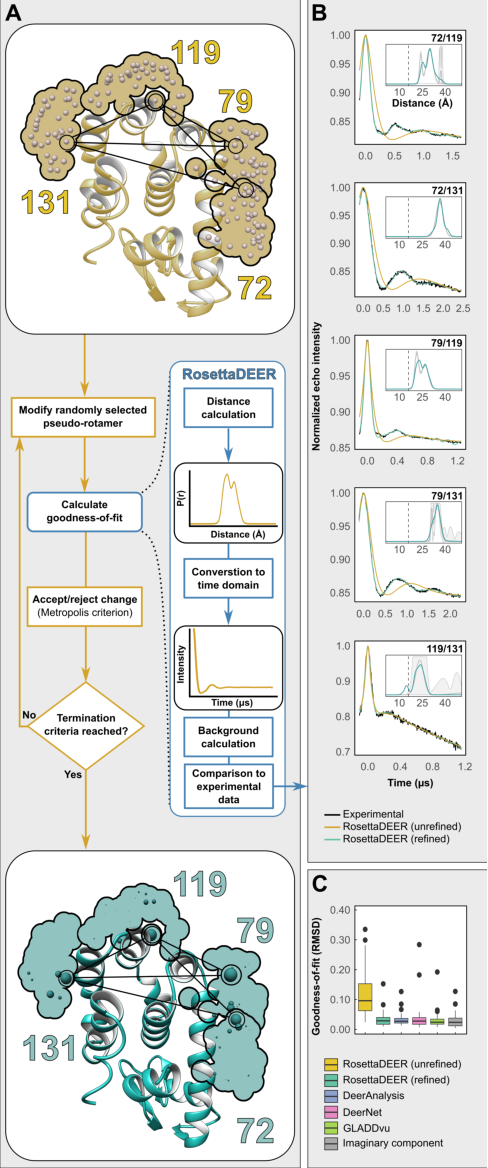
\includegraphics[width=3in]{Figures/multilateration_main_scheme.pdf}
 \caption[Overall scheme of the RosettaDEER multilateration algorithm.]{Scheme of the RosettaDEER multilateration algorithm. (A) Refinement of pseudo-rotamers using the RosettaDEER multilateration algorithm. (B) Representative \gls{deer} traces prior to and following refinement. Insets: Distributions with 95\% confidence bands. (C) Comparison of RosettaDEER to other analysis programs.}
\label{fig:multilateration_main_scheme}
\end{figure}

\subsection{Data analysis benchmark}

We benchmarked this method using experimental DEER data collected in two model proteins, T4 Lysozyme \citep*{Islam2013, Weaver1987} (PDB: 2LZM) and the \gls{mate} transporter PfMATE \citep*{Jagessar2020, Tanaka2013} in its outward-facing conformation (PDB: 6GWH). The extracellular and intracellular spin label pairs of PfMATE were treated independently since they did not share residues in common. These three \gls{deer} datasets consisted of 65 restraints between 47 residues; a subset of the restraints in T4 Lysozyme is shown in \ref{fig:multilateration_main_scheme}.A. We note that unlike the benchmarks used in other multilateration methods, these restraints were highly interconnected; half of the residues were spin labeled in three or more DEER pairs, and in the most extreme case, two residues in T4 Lysozyme were spin labeled across seven pairs (Figure \ref{fig:multilateration_supp_n_restraints}). For each of the three datasets, the RosettaDEER multilateration algorithm was executed for 1000 replicas, with each replica yielding refined pseudo-rotamer ensembles at every spin labeled site.

We compared the resulting fits to those obtained using GLADDvu \citep*{Hustedt2018}, DeerAnalysis \citep*{Jeschke2006}, and DeerNet \citep*{Worswick2018}, which are programs that analyze \gls{deer} data using Gaussian mixture models, Tikhonov regularization, and feed-forward neural networks, respectively. Although other analysis methods are available, we believe these represent a sufficiently diverse range of analytical approaches for the purposes of comparison. We found that the optimum rotamer ensembles, selected by the \gls{aicc}, could recapitulate the experimental \gls{deer} traces as effectively as each of these programs (Figures \ref{fig:multilateration_main_scheme}.B and C, \ref{fig:multilateration_supp_alltraces}, \ref{fig:multilateration_supp_gladdvu}, \ref{fig:multilateration_supp_deeranalysis}, and \ref{fig:multilateration_supp_deernet}). The mean squared errors obtained by the best fit were not statistically different from those obtained by any of these three methods, or from the noise estimated from the imaginary component (Student’s paired one-tailed t-test with Bonferroni correction). However, unlike the latter methods, the interconnectedness of the spin label pairs allowed our algorithm to couple pseudo-rotamer parametrization to the analysis of \gls{deer} data in the time domain.

\begin{wrapfigure}{R}{0.5\textwidth}
\centering
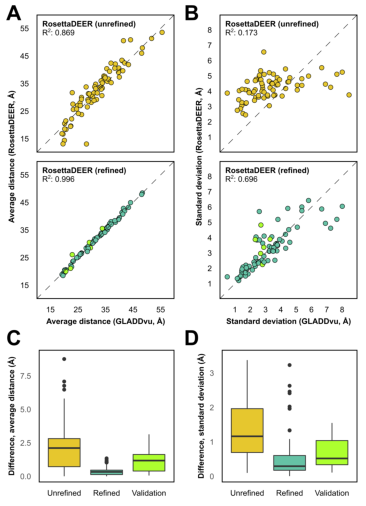
\includegraphics[width=3.25in]{Figures/multilateration_main_fit.pdf}
 \caption[Evaluation of distance distributions by multilateration.]{Evaluation of distance distributions by multilateration. Average distances (A) and widths (B) between pseudo-rotamers prior to (top) and following (bottom) refinement by multilateration. T4 lysozyme distributions omitted from multilateration are shown in light green. (C and D) Boxplots showing the difference between values obtained using GLADDvu and values simulated between pseudo-rotamer ensembles prior to and following refinement.}
\label{fig:multilateration_main_fit}
\end{wrapfigure}

\subsection{Distance distribution benchmark}

We anticipated that the analysis of \gls{deer} data by multilateration would yield distance distributions similar to those obtained using traditional methods. Consistent with this expectation, distributions between refined pseudo-rotamers in both T4L and PfMATE showed remarkable agreement with those obtained using the three methods mentioned above (see insets in Figure \ref{fig:multilateration_main_scheme}.B for examples and  \ref{fig:multilateration_supp_gladdvu}, \ref{fig:multilateration_supp_deeranalysis}, and \ref{fig:multilateration_supp_deernet} for all distributions). For example, the average values of these distributions were within \SI{0.5}{\angstrom} of those obtained using GLADDvu for 60 of the 65 restraints (Figure \ref{fig:multilateration_main_fit}). Additionally, the widths of 52 of these restraints were within \SI{0.5}{\angstrom} of those obtained using GLADDvu. Discrepancies occurred for broad distributions or long distances (because the information content in the time domain is not as well-defined) or components less than \SI{15}{\angstrom} (because these distances minimally contribute to the \gls{deer} signal). Additionally, we uncovered differences when comparing the widths of these distributions to those obtained using DeerAnalysis, likely resulting from small “ghost” side peaks frequently observed in regularization. Discrepancies were also observed when comparing these distributions to those obtained using DeerNet, which yielded widths clustered between \SIrange{2.5}{4.5}{\angstrom} (Figure \ref{fig:multilateration_supp_avgs_stdev}).

Finally, the uncertainty of these distributions was calculated from the five pseudo-rotamer ensembles with the lowest \gls{aicc} values. The resulting confidence bands, which capture 95\% of the variation in the distance distributions, are qualitatively comparable to those obtained using GLADDvu, DeerAnalysis, and DeerNet (Figure \ref{fig:multilateration_supp_conf_bands}).

To further validate the algorithm, we simulated distance distributions for six T4L spin label pairs which were excluded from the multilateration dataset. We observed that the median error between the average distance values fell by 50\% (Figure \ref{fig:multilateration_main_fit}) using the refined rotamers. By contrast, the standard deviations did not significantly sharpen, and their values are similar to those observed prior to refinement. Notably, the uncertainty of these distributions is greater than those of the distributions included in the training set.

\subsection{Conformational change modeling in PfMATE using refined pseudo-rotamers}

While the results above demonstrate the robustness of the multilateration algorithm in identifying optimal spin label pseudo-rotamer ensembles, the central question is whether these provide superior restraint quality for modeling conformational changes. To address this question, we modeled the isomerization of PfMATE between \gls{of} and \gls{if} conformations (shown in Figure \ref{fig:multilateration_main_rmsd}.A and B, respectively), both of which were determined by X-ray crystallography \citep*{Tanaka2013, Zakrzewska2019}. The two conformations differ primarily in the relative orientations of the N- and C-terminal domains resulting from changes in the backbone dihedral angles of \gls{tmh}7. Of direct relevance to the question addressed here, distance distributions between pairs of spin labels measured at pH 7.5 and pH 4.0 were shown to be consistent with the OF and IF conformations, respectively \citep*{Jagessar2020}.



We generated several thousand models, using Rosetta \citep*{Leaver-fay2011, Leman2020} without \gls{deer} restraints, by perturbing \gls{tmh}7 and found that none of the built-in membrane protein scoring functions \citep*{Alford2020, Alford2015, Weinstein2019, Yarov-Yarovoy2006} could identify the \gls{if} state by score alone (Figure \ref{fig:multilateration_supp_scores}) even if it was included in the initial model set. Thus, from an \gls{mc} modeling perspective, the \gls{of}-to-\gls{if} conformational transition can be sampled, but not necessarily identified, without experimental data.

\begin{table}[h!]
\scriptsize
%\renewcommand{\tabcolsep}{0.09cm}
\renewcommand{\tabcolsep}{0.15cm}
\centering
\caption[Restraints used to score PfMATE models.]{Restraints used to score PfMATE models.}

\newcolumntype{Y}{>{\raggedright\arraybackslash}X}

\begin{center}
\begin{tabular}{l l l l l l l l l l l}
\toprule \\
\textbf{Set} &	\textbf{1} &	\textbf{2} &	\textbf{3} &	\textbf{4} &	\textbf{5} &	\textbf{6} &	\textbf{7} &	\textbf{8} &	\textbf{9} &	\textbf{10} \\
\midrule \\
1 &	120/269 &	215/318 &	120/413 &	215/394 &	134/269 &	215/442 &	186/269 &	240/318 &	186/348 &	240/442 \\
2 &	120/413 &	215/318 &	134/269 &	215/394 &	186/348 &	215/442 &	186/269 &	240/318 &	196/348 &	240/442 \\
3 &	240/442 &	186/348 &	215/394 &	196/348 &	215/442 &	120/269 &	215/318 &	186/269 &	240/318 &	120/413 \\
4 &	215/318 &	186/269 &	240/442 &	120/413 &	240/318 &	134/269 &	186/348 &	196/348 &	215/442 &	120/269 \\
\bottomrule \\
\end{tabular} 
\end{center}




\label{tab:pfmate_restraints}
\end{table}

\begin{wrapfigure}{r}{0.5\textwidth}
\centering
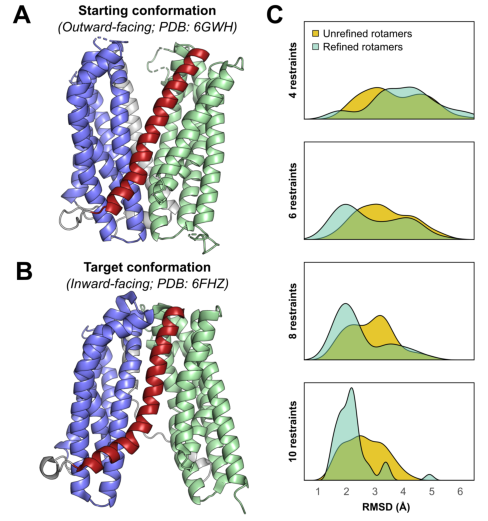
\includegraphics[width=3.25in]{Figures/multilateration_main_rmsd.pdf}
 \caption[Modeling conformational changes in the multidrug transporter PfMATE.]{Modeling conformational changes in the multidrug transporter PfMATE. (A) \Gls{of} and (B) \gls{if} crystal structures of PfMATE. N- and C-terminal domains shown in purple and green, respectively, with \gls{tmh}7 in red. (C) \Gls{rmsd} values of ten best-scoring models relative to the \gls{if} conformation using pseudo-rotamers either refined by multilateration (teal) or available by default (yellow).}
\label{fig:multilateration_main_rmsd}
\end{wrapfigure}

To test the notion that \gls{deer} restraints interpreted with the refined pseudo-rotamers can drive convergence of Rosetta modeling, we identified spin label pairs where the \gls{epr} lineshape showed minimal changes upon a pH shift from 7.5 to 4.0, supporting the approximation that the spin label rotamer ensembles are invariant and thus were not allowed to reconfigure during Rosetta modeling (Table \ref{tab:pfmate_restraints}). From these pairs, 40 sets of restraints were generated, each of which consisted of one to ten spin label pairs. Using scoring functions to assess the agreement with the DEER restraints (see section \ref{sec:multilateration_main_methods}), the \gls{of}-to-\gls{if} conformational transition was modeled by perturbing the dihedral angles of \gls{tmh}7. \Gls{deer} distributions were simulated using either the pseudo-rotamers ensembles refined by multilateration or the unrefined ensembles available to RosettaDEER by default. Agreement with the experimental distributions was evaluated by the overlap between the experimental and simulated distance distributions. Similarity to the inward-facing crystal structure was quantified by the \gls{rmsd} of the alpha carbons excluding \gls{tmh}s 1 and 7.


We observed a striking contrast between the effectiveness of the refined and unrefined ensembles (Figure \ref{fig:multilateration_main_rmsd}.C). The default rotamer library did not effectively improve the average \gls{rmsd} values of the ten lowest-scoring models beyond \SIrange{2.0}{3.5}{\angstrom}. By contrast, the use of multilaterated pseudo-rotamers converged upon inward-facing models to \SIrange{1.5}{2.5}{\angstrom} $\mathrm{C_{\upalpha}}$ \gls{rmsd} using restraints obtained from the same spin label pairs.

Alongside these improvements in accuracy, the sharper range of \gls{rmsd} values suggested that multilateration improved model precision. Distributions of representative distances in the intracellular and extracellular sides of the top ten models (Figures \ref{fig:multilateration_main_convergence}.A and B) revealed that, when using the default pseudo-rotamers, a majority of these models failed to close the extracellular cavity and were less inward-open than the \gls{of} structure (Figure \ref{fig:multilateration_main_convergence}.C), even when ten restraints were used. By contrast, models obtained using refined pseudo-rotamers deviated less drastically from the crystal structure. Nonetheless, these models were virtually all less inward-open than the crystal structure, consistent with shorter-than-expected experimental \gls{deer} measurements on the intracellular side at pH 4.0 (Figure \ref{fig:multilateration_main_convergence}.D) \citep*{Jagessar2020} .


\subsection{Concluding remarks}

Our results highlight a strategy to improve the quality of models obtained from \gls{epr} restraints. We envision that the main application of this strategy is to model alternate conformational states starting from an experimental structure and a set of interconnected \gls{deer} data. By implementing this algorithm in Rosetta, we hope to encourage its use for a wide variety of modeling applications, such as protein-protein docking and \emph{de novo} folding. Moreover, further development of this approach, as well as extensive use of multilateration in the design of spin label pairs, will open the door to modeling proteins where conformational changes are defined by more complex modes of motion.

\section{Materials and Methods}\label{sec:multilateration_main_methods}

\subsection{Overview of the model-based approach}


\begin{wrapfigure}{r}{0.6\textwidth}
\centering
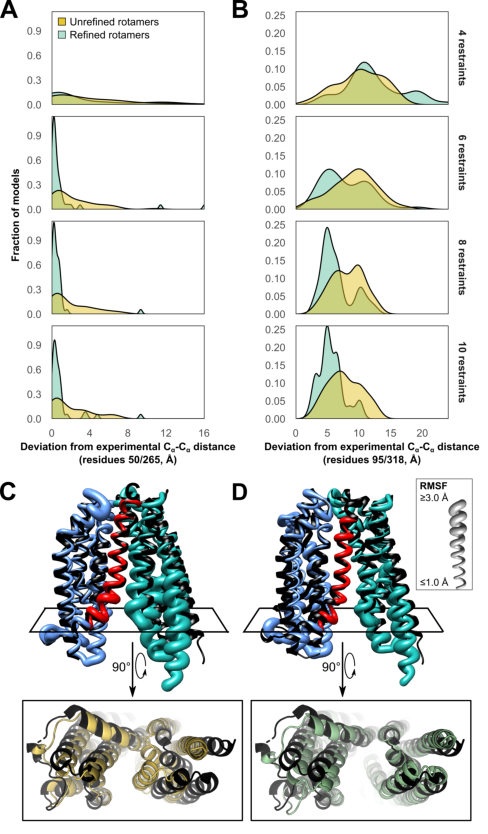
\includegraphics[width=3.25in]{Figures/multilateration_main_convergence.pdf}
 \caption[Models obtained using multilaterated rotamers more closely resemble the IF structure.]{Models obtained using multilaterated rotamers more closely resemble the IF structure. Deviation between experimental and predicted $\mathrm{C_{\upalpha}}$-$\mathrm{C_{\upalpha}}$ distances observed between pairs on the A) extracellular and B) intracellular sides. Models obtained using ten restraints either with C) default or D) refined rotamers (\gls{if} structure in black).}
\label{fig:multilateration_main_convergence}
\end{wrapfigure}

The objective of the RosettaDEER multilateration algorithm is to fit a set of \gls{deer} data by weighting the nitroxide pseudo-rotamers available to each spin-labeled residue in a protein structural model. Each replicate of the algorithm independently generates a unique set of pseudo-rotamer ensembles for each spin-labeled residue. For clarity throughout this text, we will refer to these outputs as "coordinate models", to differentiate them from the starting structural models. The space accessible to the unpaired electron of each residue’s spin label is divided into fifty discrete pseudo-rotamers, which are shown as small spheres in Figure \ref{fig:multilateration_main_scheme}.A. RosettaDEER then identifies and removes pseudo-rotamers that clash with the protein backbone. Each residue’s ensemble of pseudo-rotamers represents a probability density function of the space accessible to the unpaired electron of that residue’s spin label. As a result, following refinement using this algorithm, the weights of a coordinate model’s pseudo-rotamers for any given residue are tightly coupled to those of other residues.



In this study we focus our attention on coordinate models with high parsimony. For example, coordinate models capable of recapitulating \gls{deer} traces using only one pseudo-rotamer per residue are prioritized over those with two or more. However, if the \gls{deer} trace indicates a broad and multimodal distribution, additional pseudo-rotamers may be necessary to improve the goodness-of-fit. The total number would ideally be no greater than the minimum required to fit the data, and multiple combinations of pseudo-rotamers may be equally consistent with the data. We identified parsimonious coordinate models using the \gls{aicc} \citep*{Akaike1973, Burnham2002, Sugiura1978}:

\begin{equation}
AICc = -2 * \ln(L(\hat{\vartheta}|D)
\label{eq:aicc}
\end{equation}

This metric balances two competing objectives of 1) fitting the experimental data as well as possible and 2) simplifying the model as much as possible. The leftmost term, goodness-of-fit, is expressed as the maximum likelihood estimate of the coordinate model with parameters $\vartheta$ given the experimental \gls{deer} data $D$ and is described below. The middle and rightmost term express the complexity of the model, with the variable $K$ corresponding to the total number of parameters in the coordinate model and $n_{\mathup{total}}$ corresponding to the total number of time points in the experimental \gls{deer} data. $K$ includes the number of pseudo-rotamers with nonzero weights, as well as the number of parameters required to fit the intramolecular \gls{deer} data in the time domain. The rightmost term, which converges to zero as the data-to-parameter ratio increases, serves as further regularization in modeling cases where less experimental data is available (in this case corresponding to the number of time points in all \gls{deer} traces). Overall, the \gls{aicc} quantifies the expectation that few spin label rotamers contribute to the distance distribution.

\subsection{Detailed description of the multilateration algorithm}

The multilateration algorithm is implemented in Rosetta \citep*{Leaver-fay2011, Leman2020} as part of the RosettaDEER package and can be run using RosettaScripts \citep*{Fleishman2011}. It uses an iterative simulated annealing approach and is therefore non-deterministic. As a result, it obtains diverse sets of solutions when executed multiple times. However, there is no guarantee that the global minimum solution is obtained using this algorithm.

The positions of the pseudo-rotamers are kept fixed in space throughout the duration of the algorithm, e.g., they are reweighted, rather than moved. Initial positions are obtained from the nitroxide bond midpoints of each rotamer in the Rosetta \gls{mtssl} rotamer library following clash evaluation \citep*{Alexander2013}. At the start of the algorithm, one of these pseudo-rotamers is randomly chosen for each residue and has its weight set to 1; the rest have weights set to zero.

The algorithm then proceeds as follows:

\begin{itemize}
    \item The weight of a randomly chosen pseudorotamer is modified by a randomly chosen number. Initially this value ranges uniformly from -0.1 to 0.1.
    \item The weight change is applied, and the resulting sum-of-squared residuals is calculated as discussed below.
    \item Any move that decreases the sum-of-squared residuals is accepted, while any move that increases it is accepted with the following probability (with $\mathup{iter}$ being the current iteration):
    \begin{equation}
        p_{accept}= \exp \left( - \frac{\ln \left( L \left( \vartheta_{\mathup{iter+1}} | D \right) \right) - \ln \left( L \left( \vartheta_{\mathup{iter}} | D \right) \right) }{k_{\mathup{B}}T} \right)
        \label{eq:multilateration_accept}
    \end{equation}
    \item The Boltzmann temperature $k_{\mathup{B}}T$ starts at 1.5 and asymptotically approaches zero with each iteration as the algorithm proceeds. A total of 2500 trials per round are performed per \gls{deer} trace in the dataset. However, each round is aborted if 500 consecutive trials fail to sample an improvement.
    \item At the end of each round, the temperature $k_{\mathup{B}}T$ is raised to 1.5. If no improvements were sampled, the magnitude of the weight changes made to coordinates is reduced by a factor of $\sqrt{10}$. Once this magnitude reaches $10^{−4}$, the algorithm is concluded.
\end{itemize}

For PfMATE, we used a non-three-dimensional background model to fit the intermolecular contribution of the experimental signal. This required a modification to the algorithm in which the first round of optimization was performed using a three-dimensional background. The first time $k_{\mathup{B}}T$ was reset to 1.5, this restriction was removed. Otherwise, the dimensionality of the intermolecular background coupling was found to immediately drop to a value of 2, trapping the solution in a local minimum.

\subsection{Simulation of DEER distance distributions}

To simulate distance distributions between two spin-labeled residues u and v, pairwise distances were measured between all coordinates belonging to each residue. To account for backbone heterogeneity, each of these measurements were then broadened by a value equal to the pairwise \gls{rmsf} as inferred from the crystallographic isotropic B-factor of the residues’ $\mathrm{C_{\upalpha}}$ atoms:

\begin{equation}
    RMSF_{\mathup{u}}=\sqrt{\frac{3 B_{\mathup{u}, C_{\upalpha}}}{8 \pi^{2}}}
\end{equation}

\begin{equation}
    RMSF_{\mathup{uv}}=\sqrt{RMSF_{\mathup{u}}^{2}+RMSF_{\mathup{v}}^{2}}
\end{equation}

The result is equivalent to the convolution of the original distribution with a Gaussian distribution with a width of $RMSF_{\mathup{uv}}$. Regions of proteins with higher B-factors, such as loops, have previously been found to exhibit a greater degree of backbone flexibility in solution \citep*{Billeter1992, Powers1993, Yang2007}. Failure to account for backbone flexibility could potentially overstate the intrinsic dynamics of the spin label and decrease the precision of the models generated using the pseudo-rotamers obtained this way. We did not normalize the experimental B-factors to account for differences in experimental crystallographic resolution, since such differences may reflect variations in the backbone disorder of different proteins.

\subsection{Evaluating coordinate models obtained from raw DEER traces}

The data $D$ consist of $N$ decay traces ($V_{\mathup{exp}}$), e.g., $D = {V_{\mathup{exp,1}}, V_{\mathup{exp,2}},…, V_{\mathup{exp,N}}}$, with the $\mathup{i}$th decay trace consisting of $n_{\mathup{i}}$ time points for a total of $n_{\mathup{total}}$ experimental time points among all experimental traces. In this case, the likelihood of the model was evaluated by the noise-normalized sum-of-squared residuals to the experimental data:

\begin{equation}
    \ln \left( L \left( \vartheta | D \right) \right)=-\frac{ n_{\mathup{total}}}{2} * \ln \left( \frac{1} {n_{\mathup{total}}} \sum_{\mathup{i}=1}^{N} \sum_{\mathup{i}_{t}}^{n_{\mathup{i}}} \left( \frac{ V_{\mathup{exp,i}} \left( t_{\mathup{i_t}} \right) - V_{\mathup{intra,i}} \left( t_{\mathup{i_{t}}} | \vartheta \right) }{\sigma_{\mathup{i}}} \right)^2 \right)
    \label{eq:multilateration_loglikelihood}
\end{equation}

Here $\sigma_{\mathup{i}}$ is the standard deviation of the noise corresponding to the $\mathup{i}$th decay trace, $V_{\mathup{exp,i}}\left(t_{\mathup{i}} \right)$ refers to the experimental data at the $i_{\mathup{t}}$th time point of decay trace $\mathup{i}$, and $V_{\mathup{intra,i}}\left( t_{\mathup{i}_{t}}|\vartheta \right)$ refers to the value of the simulated data in decay trace $\mathup{i}$ at time point it given the model parameters $\vartheta$. The values of $\sigma_{\mathup{i}}$ were calculated from the imaginary component of each \gls{deer} trace. Normalizing the data to the noise was necessary to satisfy the assumption that the sum of squared residuals is independently and identically distributed. Forgoing this correction led to overfitting of noisier \gls{deer} traces and underfitting of less noisy traces.

Simulation of DEER traces occurred in three steps. First, the distance distributions were obtained from the model coordinates as described above. Second, the intramolecular form factor was calculated for each time point $t_{\mathup{i_t}}$:

\begin{equation}
    V_{\mathup{intra,t}}\left( t_{\mathup{i_{t}}} | \vartheta \right) = \sum_{\mathup{j}=1}^{m} P_{\mathup{sim,i}} \left( r_{\mathup{j}} | \vartheta \right) \int_{0}^{\frac{\pi}{2}} \sin \left( \theta \right) * \cos \left( \frac{ \left( 1 - 3 \cos^{2} \theta \right) \mu_{0} \mu_{\mathup{B}}^2 g^2 t_{\mathup{i_{t}}} }{4 \pi \hslash r_{\mathup{j}}^{3}} \right) \mathup{d} \theta
    \label{eq:multilateration_kernel}
\end{equation}

Here, $g$ is the electron g-factor, $\mu_{\mathup{0}}$ is the vacuum permeability constant, $\mu_{\mathup{B}}$ is the Bohr magneton, $t_{\mathup{i}_{t}}$ is the $i_{\mathup{t}}$th time point in microseconds, $r$ is the bin distance in nanometers, and $\theta$ is the angle between the bulk magnetic field and the interspin vector.

In the third step, the modulation depth, background slope, and dimensionality (in the case of PfMATE) were determined using nonlinear least-squares minimization. This background was modeled using the stretched exponential function $B \left( t \right) = exp \left( - \left( kt \right)^\frac{d}{3} \right)$, where $d$ refers to the dimensionality of the background coupling and was constrained to 3.0 for T4 Lysozyme and to between 2.0 and 3.5 for PfMATE. In the latter case, we generally obtained values ranging from 2.0 to 2.5. These parameters were determined using an initial search as previously described and were fine-tuned throughout the duration of the algorithm using the Levenberg-Marquardt algorithm.

\subsection{Determination of distance distributions}

We used GLADDvu \citep*{Hustedt2018} and DeerAnalysis2019b \citep*{Jeschke2006} to fit the data and obtain distance distributions. Each \gls{deer} trace was truncated by \SI{500}{ns} to avoid fitting artifacts. Sum-of-Gaussian distributions were obtained with GLADDvu using the interior point method. The distribution with the lowest Bayesian Information Criterion was selected. Distributions were also obtained using Tikhonov regularization with an L-curve criterion with default settings, as well as the generic DeerNet neural network ensemble, using DeerAnalysis2019b. Confidence bands and/or error margins were obtained using the delta method for GLADDvu, the Validation tool for Tikhonov regularization, and built-in ensemble statistics for DeerNet.

\subsection{Application to T4 Lysozyme and PfMATE}

The algorithm as described above was applied to T4 Lysozyme (PDB: 2LZM) and \gls{of} PfMATE structure (PDB: 6GWH). For PfMATE, the data were further separated into the extracellular restraints and the intracellular restraints. The algorithm was executed one thousand times for each of these three datasets. Each of the one thousand coordinate models were scored using the \gls{aicc} (Equation \ref{eq:aicc}).

\subsection{Modeling the OF-to-IF conformational change of PfMATE}

Modeling the outward-to-inward conformational change of PfMATE was achieved using an \gls{mc} fragment insertion approach implemented in RosettaScripts. This protocol randomly changes the backbone dihedral angles of certain residues chosen at random to match those of a similar stretch of residues found in protein structures deposited in the PDB. Only residues 1–50 and 241–268 were perturbed. Peptide fragments were obtained from a July 2011 version of the PDB using the Robetta web server \citep*{Kim2011} with homologous protein structures removed. The fragment insertion protocol was executed 1000 times in RosettaScripts using the \emph{score3} scoring function and was repeated for 5000 cycles. The Boltzmann temperature was set to 1.0. The following scoring function was then used to quantify the similarity between the experimental and simulated DEER distributions:

\begin{equation}
    S_{\mathup{DEER}} = \sum_{\mathup{i}=1}^{N} \ln \left( \sum_{\mathup{j}=1} p_{\mathup{sim,ij}}p_{\mathup{exp,ij}} \right)
\end{equation}

In the event that an experimental and simulated distribution did not overlap, the inner term resolves to $\ln \left(0 \right)$. Under these circumstances, this value was automatically set to -87.0, which is equivalent to the natural logarithm of the lowest non-negative value that can be described by a single-precision floating point number. The choice of this scoring function is discussed in Appendix \ref{app:scoring}.

\section{Acknowledgements}

We thank Dr. Derek P. Claxton and Dr. Richard A. Stein for critical reading of the manuscript, and Dr. Eric Hustedt for both fruitful discussions regarding the \gls{aicc} and model-based fitting as well as critical reading of the manuscript.
\clearpage % clear the prior chapter's page

\chapter{Structural dynamics of the glutamate-GABA antiporter GadC}\label{ch:gadc}
%\vspace{-7mm}
%\bigskip

This Chapter is based on unpublished data.

\section{Introduction}

Transporters belonging to the \gls{apc} family shuttle amino acids and their derivatives such as hormones and polyamines through lipid bilayers in organisms across all domains of life \citep*{Kandasamy2018, Vastermark2014}. Some \gls{apc} transporters mediate cation-independent substrate exchange, or antiport, across cell membranes \citep*{Bartoccioni2019, Errasti-Murugarren2019, Shaffer2009}, and in humans their upregulation correlates with poor prognosis in a wide variety of cancers \citep*{Kandasamy2018}.  Homologous antiporters allow bacteria to withstand extreme acid stress by importing and exporting the precursors and products, respectively, of proton-consuming amino acid decarboxylases \citep*{Foster2004, Hersh1996, Kanjee2013}. Of these four "virtual proton pumps" found in the pathogenic \emph{Escherichia coli} strain O157:H7, the \gls{glu}/\gls{gaba} antiporter GadC operates at the lowest pH range \citep*{Gao2010, Kanjee2013, Ma2012}. Unlike the others, its knockout sensitizes cells to extremely acidic conditions (pH 1.5-4.0) and sharply decreases host infection and mortality \citep*{Lu2013}. Experimental studies of GadC may thus reveal both how deadly pathogens involved in food-borne illness survive at low pH and how eukaryotic homologs with disease relevance transport their substrates.

Functional characterization of GadC revealed a stringent dependence of activity on pH, with little to no detectable transport under neutral or weakly alkaline conditions \citep*{Ma2013, Ma2012, Tsai2013}. Its structure, determined by X-ray crystallography in detergent micelles at pH 8.0, was putatively assigned to an inactivated state incapable of substrate translocation. Interestingly, a C-terminal domain unique to GadC was found embedded in the intracellular cavity, suggesting that pH-dependent inactivation appeared to be in part facilitated by autoinhibition. Although mild transport activity was observed under neutral conditions in deletion mutants lacking this domain, detachment of the C-terminus has never been directly detected.

Perhaps more importantly, the structure and dynamics of GadC as it undergoes amino acid exchange remain unknown. It has been assumed that the conformational cycles of \gls{apc} transporters are expected to follow in outline  those of well-studied LeuT-fold transporters such as neurotransmitter-sodium symporters and sodium-solute symporters, which couple the otherwise unfavorable import of substrates to inward electrochemical gradients of sodium ions \citep*{Kazmier2014a}. However, studies of these transporters using solution-state methods such as \gls{epr} spectroscopy \citep*{Claxton2010, Kazmier2014, Kazmier2014a, Paz2018} and \gls{hdxms} \citep*{Adhikary2017, Merkle2018, Moeller2019, Nielsen2019} have revealed striking divergences in both their elements of alternating access as well as its and their ligand dependence. Moreover, as symporters, \gls{nss}s, \gls{sss}s, and others undergo fundamentally different transport cycles than GadC \citep*{Forrest2009}. In contrast, the conformational dynamics of antiporters with this fold such as GadC remain understudied and unknown.

Here, \gls{deer} spectroscopy \citep*{Dastvan2019, Jeschke2012, Mchaourab2011} and integrative modeling \citep*{Rout2019, Tessmer2018} are used to investigate and model the pH-dependent structural changes of GadC in a native lipid environment. We directly detect detachment of the C-terminus at low pH and observe increases in conformational heterogeneity among neighboring helices. Unlike homologous symporters, GadC did not undergo large-amplitude substrate-dependent conformational changes at low pH, which may indicate that its antiport mechanism, rather than resulting from ligand-dependent conformational changes observed in unrelated antiporters \citep*{Jagessar2020, Martens2016, Masureel2014}, could instead stems from stabilization of a transition state that is inaccessible in the absence of substrate. Structural models generated from these distance measurements deviate from the published crystal structure in key aspects and indicate that GadC predominantly adopts an inward-facing occluded conformation in lipid bilayers \citep*{Errasti-Murugarren2019, Shaffer2009}.

\section{Results}

\begin{wrapfigure}{R!}{0.5\textwidth}
\centering
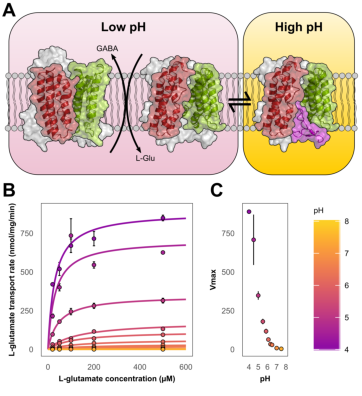
\includegraphics[width=3.25in]{Figures/gadc_main_transport.pdf}
 \caption[Transport activity in the glu/GABA antiporter GadC is dependent on pH.]{Transport activity in the glu/GABA antiporter GadC is dependent on pH. (A) Cartoon depiction of the activation mechanism. (B) Glutamate transport in wildtype GadC reconstituted into proteoliposomes is strongly dependent on pH. (C) Maximal transport rate (Vmax) increases exponentially as a function of pH.}
\label{fig:gadc_main_transport}
\end{wrapfigure}
	
The pH-dependent activity profile of GadC was verified by measuring radiolabeled substrate uptake into proteoliposomes. A construct of wildtype GadC, previously cloned from \emph{E. coli} str. O157:H7, was obtained and expressed in \emph{E. coli} C43 (DE3), purified in $\mathrm{\upbeta}$-DDM detergent micelles, and reconstituted into proteoliposomes containing \SI{5}{mM} \gls{glu} at pH 5.5. These proteoliposomes were then tested for substrate transport by detection of [$\mathrm{^3H}$]-L-glutamic acid uptake as a function of both external pH and substrate concentration. Additionally, time-dependent \gls{glu} transport was measured in proteoliposomes containing \SI{5}{mM} \gls{gaba} at pH 5.5 (Figure \ref{fig:gadc_supp_time_transport}). Consistent with previous findings \citep*{Ma2013, Ma2012, Tsai2013}, we observed a strong dependence of radioligand uptake on pH, with negligible transport detected at pH 6.5 and above (Figures \ref{fig:gadc_main_transport}.B and C).

To characterize the structural changes associated with pH-dependent activation, we used site-directed spin labeling and \gls{epr} spectroscopy \citep*{Jeschke2012, Mchaourab2011}. After mutating all three endogenous cysteines in the wildtype sequence to chemically inert residues (C60V, C247A, C380V), a panel of 25 single- and double-cysteine mutants were generated. As with previous studies on structural homologs of GadC, double-cysteine pairs were selected based on their ability to report on inter- and intra-domain motions. To evaluate if these measurements were expected to fall within the detectable range for DEER measurements (\SIrange{15}{60}{\angstrom}) and to test whether the resulting data were consistent with the crystal structure, distance measurements were first simulated between candidate residue pairs using dummy spin labels modeled over the crystal structure \citep*{Islam2013, Jo2014}. Following purification and spin-labeling, all mutants were reconstituted into proteoliposomes and tested for transport and pH-dependent inactivation at pH 5.5 (Figure \ref{fig:gadc_supp_transport}) and 7.5 (Figure \ref{fig:gadc_supp_transport75}), respectively. Additionally, all experimental \gls{deer} measurements were carried out in nanodiscs with lipid profiles matching those of the proteoliposomes used for transport assays. This ensured that neither the spin labels nor the membrane environment interfered with the protein's ability to traffic substrates at acidic pH or to undergo inactivation at neutral pH.


\begin{wrapfigure}{r!}{0.5\textwidth}
\centering
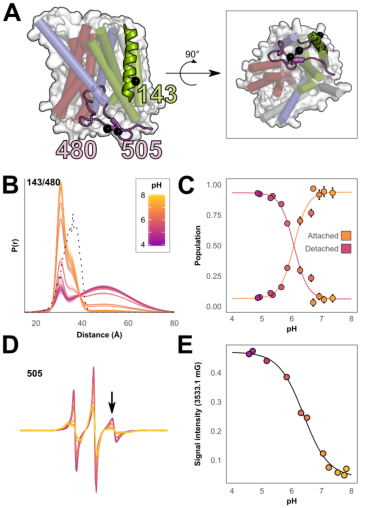
\includegraphics[width=3.25in]{Figures/gadc_main_tail.pdf}
 \caption[Detachment of the C-terminus is triggered by low pH.]{Detachment of the C-terminus is triggered by low pH. (A) Position of the C-terminus, shown in pink, relative to the main transmembrane domain of the transporter. Inset: The domain is embedded into the intracellular vestibule. (B) At low pH, a distance component consistent with a distance distribution predicted from the crystal structure (shown in the dashed line) is replaced by a wider, longer-distance component. (C) Titration measurement of the dissociation of the C-terminus. (D) pH-dependent increases in conformational heterogeneity resolved by CW-\gls{epr}. (E) Titration measurement of the third moment of the CW spectra reveals a similar profile to the DEER measurements.}
\label{fig:gadc_main_tail}
\end{wrapfigure}

Although GadC was crystallized as an antiparallel homodimer, no experimental evidence of this quaternary assembly was detected in lipid nanodiscs (shown below). Additionally, the addition of substrates induced neither large-scale conformational modulations nor changes in continuous-wave \gls{epr} lineshape data (representative pairs shown in Figure \ref{fig:gadc_supp_substrates}). As a result, the following discussion is limited to pH-dependent structural changes.

\subsection{Monitoring the detachment of the C-terminus as a function of pH}


Abrogation of transport at neutral and alkaline pH has previously been attributed to a coiled domain at the protein's extreme C-terminus (shown in pink in Figures \ref{fig:gadc_main_transport} and \ref{fig:gadc_main_tail}.A). In the crystal structure of GadC, captured at pH 8.0, this domain is embedded in the intracellular cavity and putatively obstructs closure of the intracellular gate, a prerequisite of alternating access. To test the hypothesis that this domain detaches under acidic conditions, a double-cysteine mutant (143C/480C) was generated and spin-labeled to measure the distance between the C-terminus and the transmembrane domain.  Distance distributions of this pairs reported large changes as a function of pH.  At neutral pH, the average distance matched that predicted from the crystal structure, whereas a sharp increase in both the magnitude and the width of the distribution was observed under acidic conditions (Figure \ref{fig:gadc_main_tail}.B, raw data shown in Figure \ref{fig:gadc_supp_tail}). A nonlinear least-squares fit of a sigmoid function to the amplitudes of the short- and long-distance components revealed that this shift occurred cooperatively with a pKa of 6.07±0.11 (Figure \ref{fig:gadc_main_tail}.C), with both short-distance components diminishing at low pH in a tightly correlated manner (Figure \ref{fig:gadc_supp_tail_rsq}).

To further determine if this cooperative distance change originated from  conformational disorder of the C-terminal domain, a second single-cysteine mutant was introduced near the C-terminal extreme of the domain (505C). At neutral pH, the lineshape of this mutant's \gls{cw}-\gls{epr} spectrum suggested that the domain was relatively structured, consistent with its docked conformation in the crystal structure. By contrast, reducing the pH led to a sharp spectral component that dominated the lineshape at pH 6.0 and below, suggesting increases in the C-terminal domain's disorder and mobility. Nonlinear least squares fit of the signal's intensity of the high field line on as a function of pH yielded a pKa of 6.30±0.04, consistent with the \gls{deer} measurements discussed above (Figure \ref{fig:gadc_main_tail}.D and E). Taken together, the data are consistent with the corroborate the hypothesis that the tail detaches from the transmembrane domain and becomes heterogeneous and disordered. Additionally, the pKa of this event closely matched the pH at which transport activity is abrogated, reinforcing this domain’s role in regulating substrate exchange under neutral pH conditions.
	
\subsection{Characterization of structural changes in the transmembrane domain induced by low pH}

To determine if low pH drives additional structural changes following detachment of the C-terminal domain, a systematic analysis of the structure of GadC was undertaken. A variety of motifs defining conformational heterogeneity and alternating access have been observed in structural homologs using both high-resolution methods, such as crystallography and \gls{cryoem} \citep*{Bozzi2019, Kazmier2017, Krishnamurthy2012, Lee2019, Liu2019, Perez2012, Shimamura2010,  Weyand2008, Yamashita2005, Yan2019}, as well as solution-state methods such as \gls{epr} spectroscopy \citep*{Claxton2010, Kazmier2014, Kazmier2014a, Paz2018}, \gls{fret} \citep*{Zhao2010}, and \gls{hdxms} \citep*{Adhikary2017, Merkle2018, Moeller2019, Nielsen2019}. Depending on the transporter, isomerization between inward- and outward-facing conformations appears to be largely mediated by combinations of rigid-body movements between the bundle and hash domains, movement of \gls{el}2 and unwinding of \gls{tmh}5, and/or independent movement of \gls{tmh}1, \gls{tmh}6a, \gls{tmh}7, and/or \gls{el}4. We thus set out to test if movement in these motifs underpin activation of GadC at low pH.
	
\subsection{The bundle domain is tilted relative to the crystal structure}

\begin{figure}[h!]
\centering
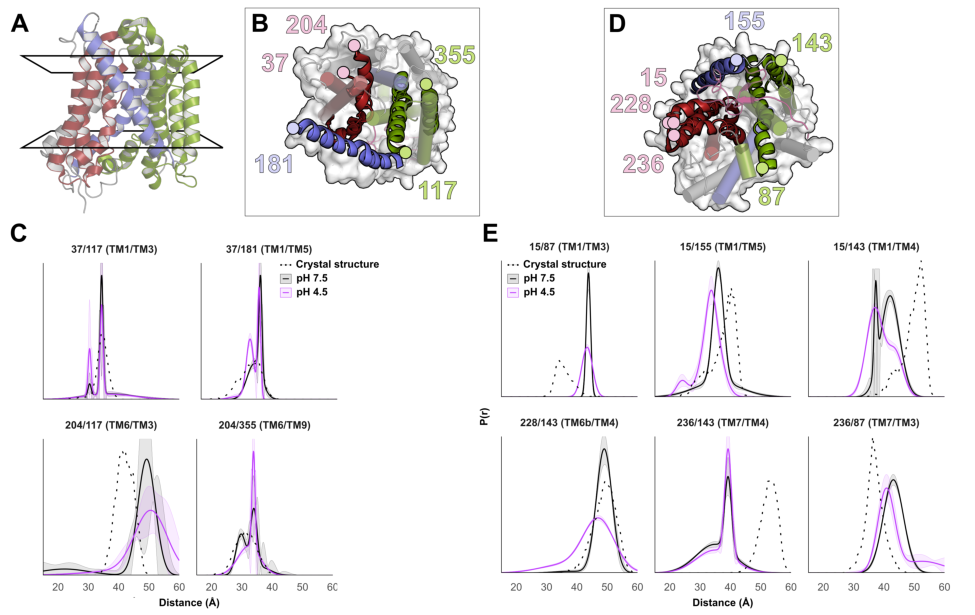
\includegraphics[width=6.5in]{Figures/gadc_main_bundle_hash.pdf}
 \caption[Distance measurements between the bundle and scaffold domains reveal deviate from crystal structure.]{Distance measurements between the bundle and scaffold domains deviate from crystal structure. (A) Side view of GadC with the top and bottom slices corresponding to panels B and D, respectively. (C) Distance measurements carried out at pH 4.5 and 7.5 alongside predictions made from the crystal structure. Confidence intervals (95\%) shown as shaded regions. (E) Distance measurements on the intracellular side reveal striking inconsistencies with the crystal structure.}
\label{fig:gadc_main_bundle_hash}
\end{figure}

A series of measurements were carried out between spin labels attached to the bundle domain and either the hash domain or \gls{tmh}5 on the extracellular side of the GadC (Figure \ref{fig:gadc_main_bundle_hash}.A). Distance distributions collected at pH 7.5 were largely in agreement with predictions made from the crystal structure, in which the extracellular gate was fully closed (Figure \ref{fig:gadc_main_bundle_hash}.B). Consistent with this finding, \gls{cw} profiles involving residue 37, located on the loop connecting helices 1 and 2, were broad and indicative of a constrained environment (Figure \ref{fig:gadc_supp_bundle_hash_extra}). Additionally, cysteine mutants labeled at this residue showed partially abrogated transport at low pH (Figure \ref{fig:gadc_supp_transport}). Only minor changes were observed in measurements at pH 4.5, suggesting that the extracellular vestibule remained closed even at low pH. Although broadening was observed between \gls{tmh}3 and \gls{tmh}6, the considerable overlap between the 95\% confidence intervals for both distributions prevented us from definitively concluding that this resulted from conformational rearrangements. The remainder of the data indicate that at both low and high pH, the extracellular gate is consistent with the outward-closed conformation observed in the crystal structure (Figure \ref{fig:gadc_main_bundle_hash}.C).

In contrast to these observations, distance measurements carried out on the intracellular side of GadC deviated substantially from predictions made from the crystal structure (Figures \ref{fig:gadc_main_bundle_hash}.D, \ref{fig:gadc_main_bundle_hash}.E, and \ref{fig:gadc_supp_bundle_hash_intra}). At pH 7.5, we observed that \gls{tmh}1 and \gls{tmh}7 in the bundle domain were \SIrange{10}{15}{\angstrom} farther from \gls{tmh}3, and \SIrange{10}{20}{\angstrom} closer to \gls{tmh}4 and \gls{tmh}5, than the predictions made from the crystal structure. Lowering the pH to 4.5 caused these distance distributions to broaden and, in some distributions, to further shorten by \SIrange{3}{5}{\angstrom}. However, the pairwise nature of the data do not immediately indicate which regions of the protein A) deviated from the crystal structure, and B) underwent increases in heterogeneity.

\subsection{The scaffold domain is largely consistent with the crystal structure}

As only minor pH-dependent movement was observed between the bundle and hash domains, subsequent measurements focused on \gls{el}4 and \gls{il}1, which connected helices 7 and 8 and 2 and 3, respectively. \Gls{el}4 has been shown to pivot outward and provide access to the extracellular vestibule in LeuT \citep*{Claxton2010, Kazmier2014a}, whereas transport activity data suggest that \gls{il}1 is involved in mediating pH-dependent activation in the homolog AdiC \citep*{Wang2014}. In addition to revealing whether the positions of these domains respond to changes in pH, the \gls{deer} data could further determine the extent to which the discrepancies observed between our measurements and predictions made from the crystal structure extended to the remainder of the structure.

\begin{figure}[h!]
\centering
\includegraphics[width=6.5in]{Figures/gadc_main_il1_el4.pdf}
 \caption[No pH-dependent movements are observed in IL1 and EL4.]{No pH-dependent movements are observed in IL1 and EL4. (A) Extracellular view of GadC. (B) Measurements between EL4 and extracellular sites on the scaffold domain suggest that TM5 is closer to the main body of the transporter than in the crystal structure. Confidence intervals (95\%) shown as shaded regions. (C) Intracellular view of GadC. (D) Intracellular measurements within the scaffold domain. (D) Intracellular view. (E) Side view. (F) In-to-out measurement suggests a slight pH-dependent movement in \gls{tmh}9.}
\label{fig:gadc_main_il1_el4}
\end{figure}

On the extracellular side, we collected three distance distributions between \gls{el}4 and various points in the structure (Figures \ref{fig:gadc_main_il1_el4}.A, \ref{fig:gadc_main_il1_el4}.B, and \ref{fig:gadc_supp_el4}). None of the distributions indicated a large-amplitude distance change as would be expected from \gls{el}4-mediated opening of the extracellular vestibule. However, whereas two of the distributions involving the C-terminal end of \gls{el}4 (residue 280) were in reasonable agreement with the crystal structure, a third pair collected between \gls{tmh}5 and \gls{el}4 showed a shorter-than-expected distance distribution. To ascertain if this discrepancy was due to the position of \gls{tmh}5, rather than \gls{el}4, we collected an additional measurement between TM3 and TM5 and found that it too was also shorter than expected (Figure \ref{fig:gadc_main_il1_el4}.A). A likely explanation is that the extracellular side of \gls{tmh}5 does not protrude as far as suggested by the crystal structure, and that the position of \gls{el}4 is otherwise consistent with the crystal structure.

Distance distributions between \gls{il}1 and \gls{tmh}3 similarly showed little movement and suggest that the two helices are effectively stapled together, consistent with a lack of independent movement observed in other LeuT-fold transporters (Figures \ref{fig:gadc_main_il1_el4}.C, D, and \ref{fig:gadc_supp_il1}). Further measurements across the hash domain on the intracellular side highlight its structural invariance. However, minor pH-dependent distance changes in \gls{il}1/\gls{tmh}4 are observed and appear to accompany local reconfigurations as evidenced by the \gls{cw} profile (Figure \ref{fig:gadc_supp_il1}). Alongside evidence that other distributions involving residue 143 on \gls{tmh}4 were bimodal, these data suggest that several distinct nitroxide rotamer states may be populated and that their relative proportions shift as a function of pH. Measurements from the hash domain to \gls{tmh}5, by contrast, do indicate minor changes in their relative positions. This further illustrates how changes in pH and detachment of the C-terminal tail domain coincide with subtle reorganizations of helices on the intracellular side of the protein.

Interestingly, measurements between \gls{il}1 and \gls{tmh}9 on the extracellular side suggested a slight sharpening that may be pH-dependent (Figure \ref{fig:gadc_main_il1_el4}.E and F). The similarity in the distance changes observed between both \gls{tmh}6/\gls{tmh}9 (204/355) and \gls{el}4/\gls{tmh}9 (280/355; Figures \ref{fig:gadc_main_bundle_hash}.A and \ref{fig:gadc_main_il1_el4}.A, respectively), combined with the lack of distance changes in measurements involving IL1, suggest that these data as slight pH-dependent movements of \gls{tmh}9. However, this movement is substantially less than what is observed in structural homologs, such as Mhp1 \citep*{Shimamura2010, Weyand2011, Weyand2008}, that use the loop connecting \gls{tmh}9 and \gls{tmh}10 as a hinge to facilitate entry and exit from the substrate-binding site.

Altogether, the data reveal minor structural rearrangements on the intracellular side but fail to precisely identify which domains are moving and which are stationary.

\subsection{The bundle domain does not behave like a rigid body}

Finally, we evaluated whether the bundle domain acted as a rigid body during this pH transition. The narrowness of this domain, combined with the \SI{15}{\angstrom} lower limit of \gls{deer}, meant that we could only answer this question using distance measurements between the intracellular and extracellular sides of the protein (Figure \ref{fig:gadc_main_bundle_only}.A). Distance changes were observed in every measurement (Figures \ref{fig:gadc_main_bundle_only}.A and \ref{fig:gadc_supp_bundle_only}), arguing against the possibility that this domain acts as a rigid body as previously posited. Additionally, they reveal minor discrepancies regarding the position of the extracellular half of \gls{tmh}6, which was hinted at by measurements described previously involving the hash domain (Figure \ref{fig:gadc_main_bundle_hash}.A).

\begin{wrapfigure}{r!}{0.5\textwidth}
\centering
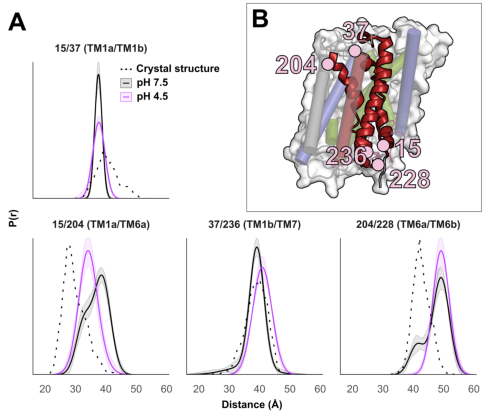
\includegraphics[width=3.25in]{Figures/gadc_main_bundle_only.pdf}
 \caption[Measurements within the bundle domains are inconsistent with a rigid-body pattern of conformational dynamics. ]{Measurements within the bundle domains are inconsistent with a rigid-body pattern of conformational dynamics. (A) In-to-out \gls{deer} distance distributions in the bundle domain. Confidence intervals (95\%) shown as shaded regions. (B) Side view showing the measurements.}
\label{fig:gadc_main_bundle_only}
\end{wrapfigure}

\subsection{GadC adopts an inward-facing occluded conformation at both pHs}

To summarize the experimental \gls{deer} data, we observed both substantial deviations between our observations and predictions made from the crystal structure, as well as minor pH-dependent broadening and amplitude changes. To translate these pairwise measurements into fold-level structural models, we generated a series of structural models of GadC using the modeling software suite Rosetta \citep*{Leaver-fay2011, Leman2020}. Unfortunately, high-precision models of the structure of GadC cannot be obtained given the relatively small number of available distance restraints. Therefore, we supplemented the modeling process with a custom-designed statistical potential that quantified each model's similarity to the structures of previously determined homologs. The design of this potential, outlined in Section \ref{sec:gadc_methods},  capitalized on the large number of structures of homologs deposited in the Protein Databank. Effectively, this statistical potential served as a form of regularization to penalize the introduction of conformational changes that are not anticipated by the known structures of closely related homologs of GadC.

We generated 5,000 Rosetta models for each pH condition using a procedure discussed in detail in section \ref{sec:gadc_methods} and Appendix \ref{app:confchangemover}. Experimental \gls{deer} data was introduced as distance restraints using the RosettaDEER module (Chapter \ref{ch:rosettadeer}) and the scoring function discussed in Appendix \ref{app:scoring}. Each model generated this way was reweighed based on its structural similarity to homologous transporters (discussed in section \ref{sec:leutintro_antiporters}). The five best-scoring models generated using data collected at either pH are shown in Figures \ref{fig:gadc_main_model}.A and \ref{fig:gadc_supp_models}. These models principally deviated from the crystal structure in the positions of \gls{tmh}1 and 7, although we note that the hash domain adopted a slightly more "upright" conformation with \gls{tmh}4 nearly parallel to the membrane normal. By contrast, the extracellular sides of these models closely resembled that of GadC, with subtle modifications to \gls{tmh}5 and \gls{tmh}6a. Initial structural comparisons suggest that these models resemble the inward-facing occluded conformation of the homologs ApcT \citep*{Shaffer2009} and MjApcT \citep*{Jungnickel2018}, in which the bundle domain is tilted toward \gls{tmh}4 and away from \gls{tmh}3 relative to the crystal structure of GadC as suggested by the data (Figure \ref{fig:gadc_main_model}). However, unlike ApcT, \gls{tmh}5 in our models is not bent or puckered and instead adopts a configuration similar to that observed in the GadC crystal structure. In fact, despite differences in the bundle domain, the overall structure of our models closely resembles the structure of GadC, highlighting both the data's limited disagreement with the crystal structure and the effectiveness of our regularization strategy.

\begin{figure}[h]
\centering
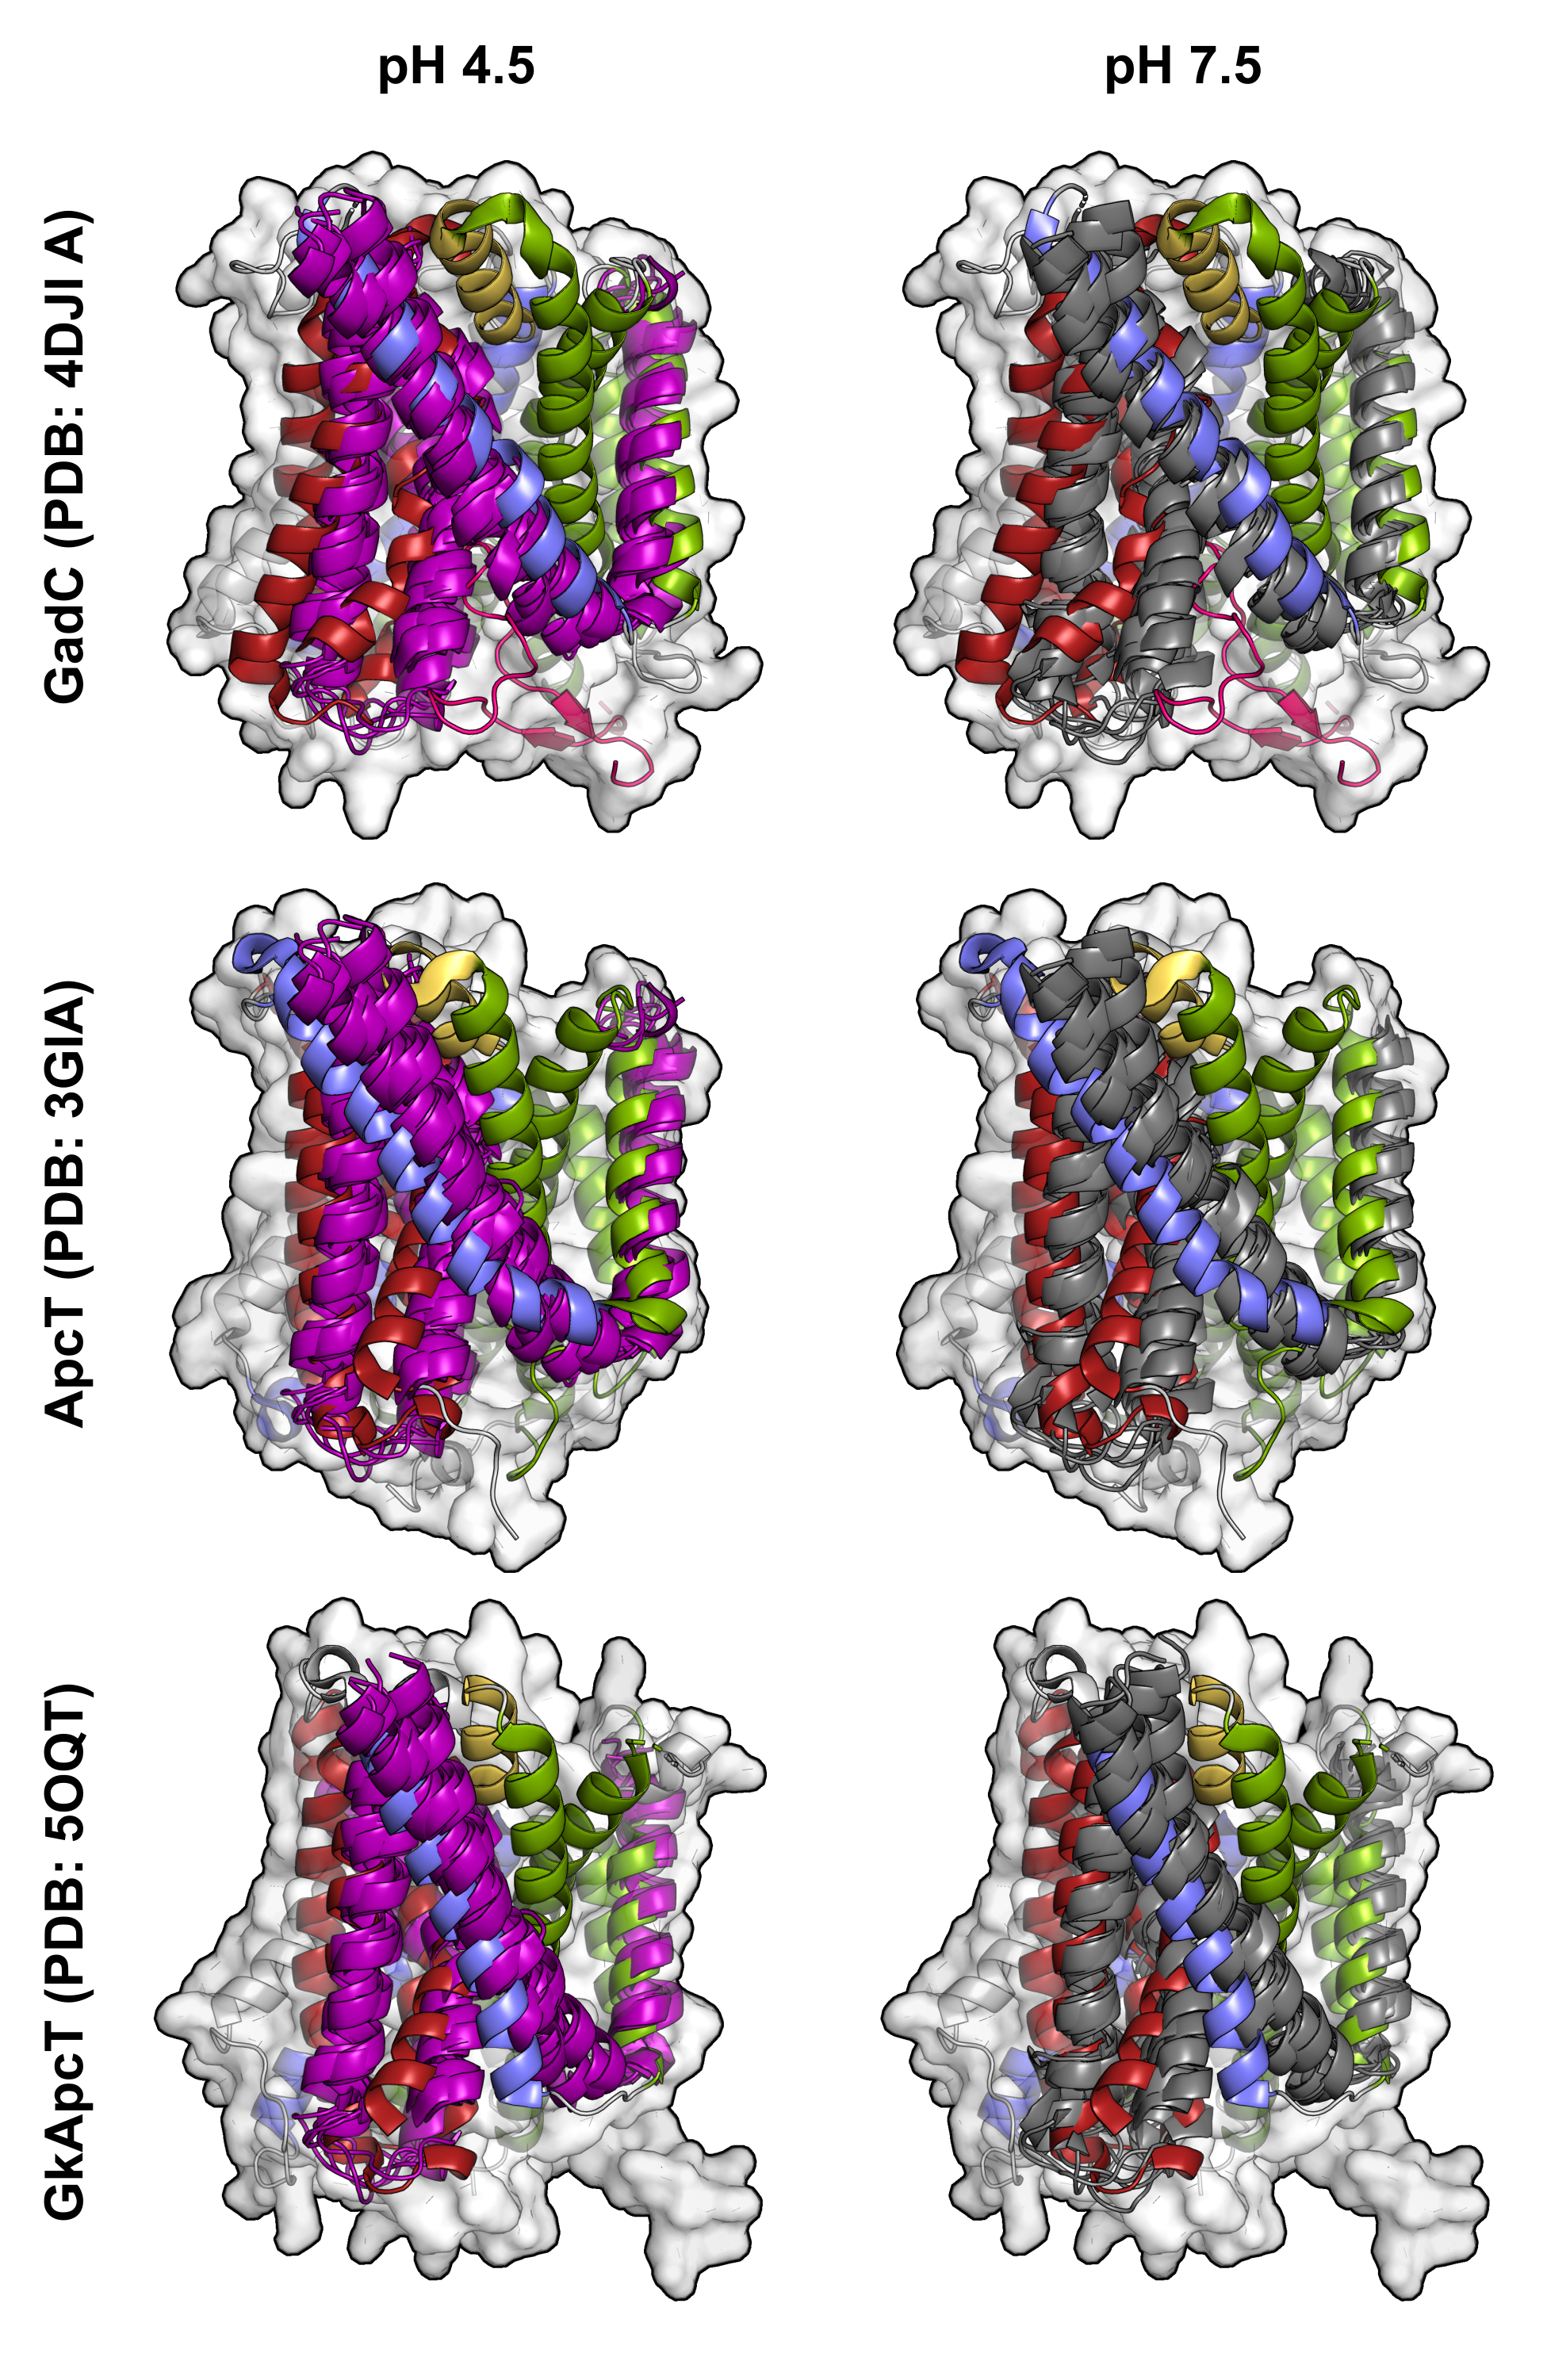
\includegraphics[width=3.25in]{Figures/gadc_main_model.pdf}
 \caption[Rosetta models of the low- and high-pH conformations generated using the DEER data in purple and dark grey, respectively.]{Rosetta models of the low- and high-pH conformations generated using the DEER data in purple and dark grey, respectively. Crystal structures of GadC and its homologs ApcT and GkApcT are shown in the colored helices and suggest that GadC adopts an inward-facing occluded conformation.}
\label{fig:gadc_main_model}
\end{figure}

These clear deviations from the crystal structure contrasted with far more subtle differences observed between low-pH and high-pH models. In fact, although small pH-dependent distance changes were observed in the data, variation between the top five models at either pH were comparable to differences between models across different pHs (Figure \ref{fig:gadc_supp_models}). Therefore, we conclude that the resolution and sparseness of the data prevent the structural basis of pH-dependent activation following release of the C-terminus from being determined with high confidence. It is therefore unclear if increases in heterogeneity observed at low pH are the result of movement in \gls{tmh}5, as suggested by structures of homologous transporters, or \gls{tmh}1, which is more strongly supported by the \gls{deer} data. 

\section{Discussion}\label{sec:gadc_discussion}

The \gls{deer} data presented here investigates the structure and dynamics of the pH dependent \gls{glu}/\gls{gaba} antiporter GadC at low pH. These measurements, which reflect solution-state backbone dynamics \citep*{Jeschke2012, Kazmier2017}, are inconsistent with the conformation stabilized by the crystal lattice, with substantial deviations observed on the intracellular side of the protein. Instead, models generated using Rosetta suggested that GadC adopts a conformation similar to closely related homologs in which its the intracellular vestibule of GadC is partially occluded and resemble the inward-facing occluded conformations observed in the closely related homologs. Indeed, we found that a model of GadC generated \emph{de novo} using the state-of-the-art method RoseTTAFold \citep*{Baek2021} generated a similarly \gls{if}-occluded model that was more consistent with the data than the crystal structure \ref{fig:gadc_supp_rosettafold}. This conformation is all the more notable given the crystal structure's similarity to homologs such as BasC \citep*{Errasti-Murugarren2019}, Lat-1 \citep*{Lee2019, Yan2019}, Lat-2 \citep*{Yan2020}, and $\mathrm{b^{(0,+)}AT1}$ \citep*{Wu2020, Yan2020a}. It should be noted, however, that our measurements reflect the structure and dynamics of GadC in a more physiologically relevant lipid environment. The aforementioned homologs, by contrast, were structurally characterized in detergent micelles and/or when bound to antibodies. It should be noted that lipid/detergent-dependent conformational changes have also been reported in several transporters, including the structural homolog LeuT \citep*{Quick2009, Sohail2016}, as well as other membrane proteins. 

The absence of substrate-induced conformational changes observed at low pH (Figure \ref{fig:gadc_supp_substrates}) contrasts with results from similar studies of unrelated antiporters, such as those mediating sodium- or proton-dependent drug efflux. However, this discrepancy may be explained by the fact that, unlike the substrates of ion coupled antiporters, neither glutamate nor GABA are hypothesized to move down their concentration gradients under physiological conditions. This owes to bacterial responses to acid stress that trigger rapid decarboxylation and depletion of cytoplasmic amino acids, such as glutamate, and the corresponding spike in cognate polyamines, such as GABA \citep*{Foster2004, Richard2004}. In fact, all four of the "virtual proton pumps" involved in bacterial acid resistance, including GadC, are co-transcribed with corresponding amino acid decarboxylases \citep*{Kanjee2013}. This metabolomic adaptation ensures that neither half of GadC's transport cycle, glutamate import or GABA export, is energetically unfavorable. This, in turn, may would obviate the need for ligand-dependent changes in thermodynamics equivalent to, for example, the pH-dependent conformational rearrangements observed in proton/drug antiporters \citep*{Dastvan2016a, Jagessar2020, Masureel2014}.

On the basis of this observation, we propose a model in which the transport cycle of GadC consists of two half-cycles of uniport in which facilitated diffusion of both \gls{glu} and \gls{gaba} are coupled in opposite directions (Figure \ref{fig:gadc_main_transportmodel}). This posits that substrate binding contributes to the kinetics, rather than the thermodynamics, of the transporter's functional cycle. We propose that this is achieved by stabilization of a high-energy transition state separating the inward-facing and outward-facing conformations that, under apo conditions, cannot be traversed. Ligand-induced increases in conformational flexibility, which would be consistent with this hypothesis, have previously been reported in the homologous serine/threonine exchanger SteT using single-molecule dynamic force spectroscopy \citep*{Bippes2009}. These findings could extend to homologous amino acid exchangers in humans, such as xCT, which couples the energetically favorable export of glutamine to the import of cystine, which is immediately reduced to two cysteine molecules and thus absent from the cytoplasm \citep*{Oda2020}.

\begin{figure}[h!]
\centering
\includegraphics[width=3.75in]{Figures/gadc_main_transportmodel.pdf}
 \caption[Mechanistic model of pH-dependent activation and substrate transport in GadC.]{Mechanistic model of pH-dependent activation and substrate transport in GadC. (A) Under acidic conditions, the C-terminal domain of GadC detaches. Separately, GadB decarboxylates intracellular glutamate into GABA, consuming protons and increasing intracellular pH. (B) GadC undergoes two half-cycles of energetically downhill uniport. High cytoplasmic concentrations of GABA ensure that its export is the most energetically favorable means of undergoing \gls{if}-to-\gls{of} isomerization, while low cytoplasmic concentrations of glutamate ensure that its import is the most energetically favorable means of undergoing \gls{of}-to-\gls{if} isomerization.}
\label{fig:gadc_main_transportmodel}
\end{figure}

Nevertheless, as these conclusions are derived from data collected under equilibrium conditions, they do not reflect structural changes induced by  substrate in the presence of gradients, such as those reported in structural homologs such as SGLT1 \citep*{Loo1998}. The possibility that the conformational dynamics of \gls{apc} transporters are responsive to gradients is reinforced by evidence that homologous transporters preferentially bind substrates on specific sides of the membrane \citep*{Bartoccioni2019}. For this reason, further inquiries must determine the structure and function of GadC as it operates in and maintains a pH gradient.

\section{Materials and Methods}\label{sec:gadc_methods}

\subsection{Site-directed mutagenesis}

A codon-optimized version of the GadC gene from \emph{Escherichia coli} str. O157:H7 (Genscript) was cloned into a pET19b vector encoding an N-terminal deca-histidine tag. A cysteine-less construct (C60V, C246A, C380V) was generated from this template using site-directed mutagenesis (QuikChange). All single- and double-cysteine mutants were similarly generated from this cysteine-free construct and verified by Sanger sequencing using both T7 forward and reverse primers.

\subsection{Expression, purification, and spin labeling of GadC}

Plasmids encoding either wildtype or mutant GadC were transformed into competent \emph{E. coli} str. C43 (DE3) cells and overexpressed in 1L minimal media A supplemented with ampicillin (Gold Biotechnology) as previously described60. Upon reaching an absorbance (OD600) of 0.7-0.8, GadC expression was induced by adding \SI{1}{mM} IPTG (Gold Biotechnology) and the temperature was dropped to 20°C. Cells were harvested after 16 hours by centrifugation at \SI{5500}{g} for 15 minutes, resuspended in \SI{22}{mL} lysis buffer (\SI{100}{mM} KPi, \SI{10}{mM} DTT, pH 7.5), and lysed by sonication. After centrifugation at \SI{9000}{g} for 15 minutes, the supernatant was collected and ultracentrifuged at \SI{200000}{g} for \SI{90}{minutes}.

The pelleted membrane fractions were then solubilized in resuspension buffer (\SI{50}{mM} Tris/Mes, \SI{200}{mM} NaCl, 20\% glycerol, \SI{1}{mM} DTT, pH 7.5) containing 1\% $\mathrm{\upbeta}$-DDM (Anatrace) and stirred on ice for \SI{60}{minutes}. Insoluble material was removed by ultracentrifugation at \SI{200,000}{g} for \SI{30}{minutes}, and the supernatant was incubated with \SI{1.0}{mL} Ni-NTA Superflow (Qiagen) resin at 4°C for two hours with \SI{25}{mM} imidazole. After washing with ten column volumes of resuspension buffer containing \SI{50}{mM} imidazole and 0.05\% B-DDM, purified GadC was eluted from the resin using resuspension buffer with \SI{250}{mM} imidazole and 0.05\% β-DDM.

Following the addition of \SI{60}{mM} Mes, single- and double-cysteine mutants were labeled with three rounds of 20-fold molar excess \gls{mtssl} (Enzo Life Sciences) per cysteine at room temperature and moved to ice overnight after four hours. Samples were then concentrated using Amicon Ultra \SI{50,000}{MWCO} filter concentrators (Millipore) to a final concentration no greater than \SI{3}{mg/ml}, as reported by absorbance at \SI{280}{nm} ($\epsilon$=\SI{67,840}{M^{-1}.cm^{-1}}), and purified into \SI{200}{mM} Tris/Mes, pH 7.2, 20\% glycerol, 0.05\% $\mathrm{\upbeta}$-DDM by size exclusion chromatography using a Shodex KW-803 column with guard column. Peak fractions were isolated for further studies.

\subsection{Reconstitution of GadC into proteoliposomes}

A 3:1 ratio (weight/weight) of \emph{E. coli} polar lipids and L-$\mathrm{\upalpha}$-phosphocholine (Avanti Polar Lipids) were dissolved in chloroform and evaporated with a rotary evaporator. After overnight desiccation in a vacuum chamber, lipids were resuspended in the appropriate buffer, homogenized by ten cycles of freeze-thawing, and stored in small aliquots at -80°C.

Lipids prepared for liposomes were resuspended in \SI{25}{mM} KPi, \SI{150}{mM} KCl pH 5.5, and either \SI{5}{mM} L-Glu or \SI{5}{mM} \gls{gaba} to a final concentration of \SI{20}{mg/ml} (\SI{16.4}{mM}). Before reconstitution, lipids were diluted and destabilized with the addition of 1.25\% \gls{bog} (Anatrace) and extruded through a \SI{400}{nm} membrane filter (Whatman). Purified GadC was added to the sample at a 1:200 ratio (weight/weight), bringing the final lipid concentration to \SI{5}{mg/mL}. Following a thirty-minute incubation at room temperature, detergent was removed from the sample by the gradual addition of \SI{400}{mg/mL} SM-2 polystyrene Bio-Beads (Bio-Rad) over the course of four hours. After rocking overnight in the dark, the proteoliposome solution was cleared of biobeads and ultracentrifuged at \SI{150,000}{g} for \SI{60}{minutes}. Proteoliposomes were then resuspended in external buffer (\SI{25}{mM} KPi, \SI{150}{mM} KCl, pH 5.5) and ultracentrifuged to remove external substrates. After repeating this ultracentrifugation step a total of three times, proteoliposomes were suspended in external buffer at a final lipid concentration of \SI{100}{mg/ml}. GadC concentration was then quantified using SDS/PAGE and densitometry (ImageJ v. 1.53g), with purified GadC in $\mathrm{\upbeta}$-DDM serving as a standard curve.

\subsection{Transport assays}\label{sec:gadc_transport_assay}

\emph{In vitro} transport assays were carried out either in triplicate (concentration-dependent) or in duplicate (time-dependent) as previously described \citep*{Ma2012}. An additional baseline measurement was performed on ice. Glutamic acid (between \SI{25}{\upmu M} and \SI{1}{mM}) was added to external buffer and checked for pH immediately prior to all transport experiments. For the time-dependent transport \gls{glu}/\gls{gaba} exchange assays shown in Figure \ref{fig:gadc_supp_time_transport}, an fixed external \gls{glu} concentration of \SI{50}{\upmu M} at pH 5.5 was used. In both experiments, proteoliposomes (\SI{2}{\upmu L}) were added to external buffer (\SI{98}{\upmu L}) containing \SI{1}{\upmu Ci} [$\mathrm{^3H}$]-L-glutamic acid (approximately \SI{200}{nM}) and gently agitated. For titration experiments on wildtype GadC, proteoliposomes (\SI{1}{\upmu L}) were added to external buffer (\SI{99}{\upmu L}) containing \SI{1}{\upmu Ci} [$\mathrm{^3H}$]-L-glutamic acid. Substrate uptake proceeded for two minutes at 25°C and was quenched by adding ice-cold stop buffer (\SI{25}{mM} glycine, \SI{150}{mM} KCl, pH 9.5) and vacuum-filtering the solution through a \SI{0.22}{\upmu m} GSTF filter (Millipore) pre-soaked in stop buffer. The filter was then washed with an additional \SI{6}{mL} stop buffer, removed, and added to \SI{5}{mL} Ecoscint H scintillation solution (National Diagnostics). Following quantitation, data were analyzed using Michaelis-Menten kinetics using the \emph{curve\_fit} function implemented in SciPy \citep*{Virtanen2020}. Baseline measurements were subtracted from the 25°C measurements.

\subsection{Reconstitution of GadC into lipid nanodiscs}

Lipids for nanodisc reconstitution were prepared as described above and resuspended in \SI{50}{mM} Tris/Mes pH 7.5 to a final concentration of \SI{20}{mM}. MSP1D1E3 was purified as previously described \citep*{Jagessar2020}. Nanodisc reconstitution proceeded using a molar ratio of 1:8 GadC:MSP1D1E3, 1:50 MSP1D1E3:lipid, and 1:5 lipid:cholate. Detergents were gradually removed from the solution using SM-2 Bio-Beads as previously described \citep*{Jagessar2020}. After overnight incubation, biobeads were removed from the solution using a \SI{0.20}{\upmu m} filter. Nanodisc-reconstituted GadC was then isolated from empty nanodiscs by size-exclusion chromatography using a Superdex 200 Increase 10/300 GL column into \SI{50}{mM} Tris/Mes, pH 7.5, 10\% glycerol and concentrated using an Amicon Ultra \SI{100,000}{MWCO} filter concentrator (Millipore). The pH of all protein samples was carefully determined using a microelectrode and adjusted using \SI{1}{M} citrate and \SI{1}{M} Tris. Protein concentration was then evaluated using \gls{cw} \gls{epr} spectroscopy as previously described \citep*{Zou2010}. Glycerol was added to all \gls{deer} samples to a final concentration of 23\% vol/vol, which were then flash-frozen in liquid nitrogen prior to DEER spectroscopy.

\subsection{CW-EPR and DEER spectroscopy and data analysis}

Spin-labeled GadC was characterized using \gls{cw}-\gls{epr} at 25°C using a Bruker EMX spectrometer operating at a frequency of \SI{9.5}{GHz}, a \SI{10}{mW} incident power, and a modulation amplitude of \SI{1.6}{G}. \Gls{deer} measurements were carried out using a dead-time free four-pulse protocol \citep*{Pannier2000} at either \SI{50}{K} (for 143C/480C) or \SI{83}{K} (all other double-cysteine mutants). Pulse lengths were as follows: \SIrange{10}{14}{ns} (first $\frac{\pi}{2}$ pulse), \SI{20}{ns} (second and fourth $\pi$ pulse), and \SI{40}{ns} (third $\pi$ pulse). The pump and observation frequencies were separated by \SI{62.26}{MHz}. Echo decay data were analyzed into distance distributions using GLADDvu with the last \SI{500}{ns} of the signal truncated \citep*{Hustedt2018}. Fitting model parameters were chosen using the Bayesian Information Criterion. To analyze the pH titration distance data collected using GadC 143C/480C, the long-distance component was isolated from the two short-distance components, and was fitted with a sigmoid function using the \emph{curve\_fit} function as implemented in SciPy \citep*{Virtanen2020}. For all \gls{deer} pairs, the distance distributions were compared to predictions generated by MDDS, which was accessed using the CHARMM-GUI web server \citep*{Jo2014}.

\subsection{Generation of a structure-based statistical potential}\label{sec:gadc_potential}

After manually isolating the ten core transmembrane helices defining the LeuT-fold, each protein was aligned to each other using TM-Align version 20180426 \citep*{Zhang2005}. For each model, the highest TMscore \citep*{Zhang2004} to a transporter in the \gls{apc} family was obtained. TMscore quantifies structural similarity and ranges from 0 to 1, with 1 indicating perfect structural overlap \citep*{Xu2010}; values between different structures of the same transporter were not considered. To reflect the probability of a model belonging to the \gls{apc} family given its TMscore to structures of other proteins in that family, we used the following exponential function:

\begin{equation}
    p(M)=\exp \left( -\frac{1\mathrm{-}TMscore}{\upbeta} \right)
\end{equation}
This function was parametrized by minimization of the total cross-entropy $-\sum{\ln \left(q_i\right)}$, where $q_i=p(M_i)$ for all \gls{apc} transporters and $q_i=1-p(M_i)$ for all non-\gls{apc} LeuT-fold transporters. Using the \emph{minimize} function implemented in SciPy \citep*{Virtanen2020}, a value of $\upbeta=0.072185$ was obtained.

\subsection{Initial homology modeling}

Structural alignments were obtained using TMAlign. The Rosetta application \emph{partial\_thread} was then used to thread the first ten transmembrane helices (residues 1-359) of the GadC sequence over each structure. The three remaining helices were then directly grafted onto the structure by structural alignment; the C-terminal tail (residues 471-511) was omitted. Homology models were constructed using HybridizeMover \citep*{Song2013} with five randomly selected templates as well as the hash domain from GadC (PDB: 4DJI chain A). The weight of the \gls{deer} data was set to 10.0 during the first two stages and to 0.0 during the final full-atom minimization stage. Sequence fragments used during this step were obtained from the Robetta web server \citep*{Kim2004}. Each of these models were further refined using ConfChangeMover as described below.

\subsection{Conformational change modeling using ConfChangeMover}

The structural modeling method ConfChangeMover, described in detail in Appendix \ref{app:confchangemover}, was implemented in Rosetta 3 \citep*{Leaver-fay2011, Leman2020} and consisted of three stages. In the first stage, rigid-body segments consisting of either beta-sheets or individual helices were identified, and cutpoints were introduced in the loops connecting them. This allowed secondary structural elements to be manipulated in three-dimensional space while avoiding the "lever-arm effect" described previously \citep*{Tyka2012}. Sampling consisted of either rigid-body movements or fragment insertions. The former consisted of random rotations and translations, with an average rotation of 15° and an average translation of \SI{2.0}{\angstrom}, and the latter consisted of modifications to the backbone dihedral angles of the model. During testing, it was found that 50,000 total rounds, consisting of an even mixture of fragment insertions and rigid-body movements, was sufficient to sample a reasonable variety of conformations.

In the second stage, loops were closed using a fragment-based protocol described in detail elsewhere \citep*{Song2013}. During this stage, sequence fragments were superimposed over regions of the protein with chainbreaks that were introduced during rigid-body movement, and Cartesian minimization was used to both minimize bond lengths and correct bond angles \citep*{Rohl2004}. Additionally, contiguous regions up to fifteen residues in length were periodically taken from the starting structure and superimposed as fragments this way. We found that 1000 sampling rounds were sufficient to resolve the chainbreaks caused by the first stage.

Lastly, explicit full-atom side chains were added to the model, which was then minimized using FastRelax. An implicit membrane was introduced using RosettaMembrane \citep*{Yarov-Yarovoy2006}, with membrane-spanning regions determined using OCTOPUS \citep*{Viklund2008}.

Several types of restraints were used to drive the model toward conformations consistent with the \gls{deer} data while maintaining the LeuT-fold topology of the starting model. During the first two stages, models were restrained using the experimental \gls{deer} restraints as implemented in RosettaDEER. A weight of 10.0 was given to this score term. Agreement with the experimental distribution was quantified using the probability function:

\begin{equation}
    S_{\mathup{DEER}} = \sum_{\mathup{i}=1}^{N} \ln \left( \sum_{\mathup{j}=1} p_{\mathup{sim,ij}}p_{\mathup{exp,ij}} \right)
\end{equation}

This function reflects the overlap between the experimental and simulated distributions. In the event that any individual simulated distribution does not overlap with its experimental counterpart, the innermost term resolves to $\ln(0)$. To avoid arbitrarily large scores, we automatically set this number to -87.0, which is approximately the negative logarithm of the smallest non-negative value that can be represented by a single-precision floating point number.

To account for the relative invariance of backbone dihedral angles in experimentally observed conformational changes, the model's backbone dihedral angles $\phi_{\mathup{sim}}$ and $\psi_{\mathup{sim}}$ in radians were restrained using the following circular sigmoid functions:

\begin{equation}
    S_{\upphi}(x) = \left( 1 + \exp \left( | \phi_{\mathup{sim}} - \phi_{\mathup{exp}} | - \frac{\pi}{2} \right) \right)^{-1} + \left( 1 + \exp \left( | \phi_{\mathup{sim}} - \phi_{\mathup{exp}} | + \frac{\pi}{2} \right) \right)^{-1}
\end{equation}

\begin{equation}
    S_{\uppsi}(x) = \left( 1 + \exp \left( | \psi_{\mathup{sim}} - \psi_{\mathup{exp}} | - \frac{\pi}{2} \right) \right)^{-1} + \left( 1 + \exp \left( | \psi_{\mathup{sim}} - \psi_{\mathup{exp}} | + \frac{\pi}{2} \right) \right)^{-1}
\end{equation}

Here $\phi_{\mathup{exp}}$ and $\psi_{\mathup{exp}}$ refer to the backbone dihedral angles in the starting model. This potential minimized the introduction of unnecessary changes to backbone dihedral angles resulting from fragment insertion. These potentials were further limited to regions of the protein with secondary structure during the first stage and to loops during the second stage.

Finally, between the first two stages of modeling, coordinate constraints were placed on the $\mathrm{C_{\upalpha}}$ backbone atoms belonging to secondary structures. This minimized the probability of reversion to the initial starting pose. Both the dihedral and coordinate constraints were maintained during the full-atom minimization and were given weights of 1.0 throughout conformational change modeling.

\clearpage % clear the prior chapter's page

\chapter{Perspectives and future directions}\label{ch:conclusions}
%\vspace{-7mm}
%\bigskip

\section{Synopsis of experimental findings}

% Talk about dynamics in the LeuT-fold
% Talk about advances in modeling using EPR data
% Talk about more general advances in protein modeling

This document presents experimental research into the pH-dependent activation mechanism and conformational dynamics of GadC, a "virtual proton pump" found in the \gls{apc} transporter family. Additionally, it describes a series of structural models generated using these experimental data that attempt to recapitulate the conformation adopted by GadC in solution. While the structural dynamics of more distant homologs, such as prokaryotic and eukaryotic \gls{nss}s and \gls{sss}s, continue to be extensively studied, prior to this research only a single investigation in a member of the \gls{apc} family, the homologous serine/threonine antiporter SteT, had been conducted. It is noteworthy that although the work discussed in this dissertation coincided with several breakthroughs in membrane protein structural biology (discussed below), our body of knowledge with respect to structural dynamics of LeuT-fold antiporters barely grew. High-resolution structures of eukaryotic exchangers with disease relevance, including Lat1 and Lat2, were unaccompanied by detailed descriptions of how or even whether they isomerize when bound to ligands.

Given the sensitivity of structural homologs LeuT, Mhp1, and vSGLT to ligands, it came as a surprise that no ligand-dependent conformational dynamics were observed in GadC. Sodium-coupled symporters rely on ion gradients to drive the energetically unfavorable uptake of amino acids and other nutrients into the cell. By contrast, in the low-pH conditions under which GadC is hypothesized to be active, depletion and buildup of intracellular glutamate and \gls{gaba}, respectively, lead both substrates to be transported down their concentration gradients. The environmental concentrations of both substrates on either side of the cell may thus be sufficient to enforce productive substrate movement required by the bacterial cell under low-pH conditions. Thus, the data presented in Chapter \ref{ch:gadc} and Appendix \ref{app:gadc_supp} of this dissertation reinforce the structural and conformational diversity of transporters with the LeuT-fold, further highlighting the extent to which the energy landscapes of proteins with the same fold can diverge. A key takeaway from this work is that experimental evidence of ligand-dependent conformational dynamics in one transporter may not fully correspond with those of structural homologs; in other words, conservation of transporter dynamics at the family-level may not be guaranteed. An important implication of this conclusion is that it may suggest that the conformational dynamics of transporters in eukaryotic organisms in general and humans in particular may not match those of bacterial model systems (see section \ref{sec:leutintro_homologs}). For this reason, it remains unclear whether these results extend to human amino acid exchangers with disease relevance such as Lat1 \citep*{Lee2019, Yan2019} or xCT \citep*{Oda2020}. Ultimately this hypothesis will be tested as investigations into human proteins become more widespread.

\subsection{Perspectives on the effect of substrates on the conformational dynamics of GadC}

The \gls{deer} data presented here suggests that neither substrate biases the conformational dynamics of GadC, a finding which led us to postulate that glutamate and \gls{gaba} affect the protein's kinetics, rather than its thermodynamics - such a mechanism would almost certainly be missed by measurements carried out using the \gls{deer} technique. Under the proposed mechanism, which is outlined in section \ref{sec:gadc_discussion}, the contribution of substrate binding to conformational dynamics is limited to stabilization of a hypothetical high-energy transition state that is not traversable under apo conditions. This model, although simple, would explain both the antiport mechanism forbidden substrate-free isomerization as well as the absence of any substrate-mediated changes in the conformational dynamics of GadC observed using \gls{deer}. Nevertheless, as the \gls{deer} technique only interrogates protein thermodynamics, rather than kinetics, other experiments would be required to test this hypothesis. Direct evaluation of changes in protein kinetics can be achieved using \gls{hdxms} \citep*{Oganesyan2018}, single-molecule \gls{fret} \citep*{Schuler2013}, or fluorine \gls{nmr} \citep*{Manglik2015}.

\subsection{Perspectives on the pH-dependent activation mechanism of GadC}

This directly ties into outstanding questions regarding the mechanism of pH-dependent substrate transport. Data collected in radioligand transport assays show how activity spikes at low pH and does not appear to plateau in the pH range under experimental observation (Figure \ref{fig:gadc_main_transport}.B and C). By contrast, detachment of the C-terminus appears to occur with a pKa of 6.0 to 6.25 (Figure \ref{fig:gadc_main_tail}.B, C, and D), which likely rules out the contribution of this domain to the increase in transport rate observed at pH 4.0-5.0. In fact, the change in glutamate exchange observed at pH 6.0-6.5 is negligible compared to the high rates of transport observed at lower pHs, which calls into question the role of this domain in regulating transport at neutral pH.

Two questions naturally follow this line of thinking. First, what other mechanism could explain the pH-dependent activity observed in GadC? Although protonation of the substrates' $\mathrm{\upgamma}$-carboxylate (pKa: 4.25), a prerequisite for transport, may partially explain this phenomenon, abrogated transport of glutamine, which mimics protonated glutamate, at neutral and alkaline pHs is inconsistent with this hypothesis \citep*{Ma2013}. In the homologous arginine/agmatine antiporter AdiC, activation has been attributed to the proton sensing residue tyrosine Y74, located on the intracellular amphipathic helix connecting \gls{tmh}s 2 and 3 \citep*{Wang2014}. Whereas the wildtype similarly undergoes inactivation at neutral pH, AdiC-Y74A maintained high transport activity regardless of pH. This research is relevant because AdiC-Y74F maintained the same pH-dependent inactivation profile of the WT, and in GadC a phenylalanine is found at the equivalent position (residue 76). However, we note that spin-labeled cysteine mutants at residue 77 showed little to no change in either \gls{deer} distance measurements or \gls{cw} spectra, and was inactive at neutral pH. Nevertheless, this hypothesis can be directly tested on F76A background mutants using radioligand transport assays such as those outlined in section \ref{sec:gadc_transport_assay}. A second hypothesis in AdiC, proposed following \gls{md} simulations, suggests that protonation of E218 drives dissociation of the substrate from the active site \citep*{Zomot2011}. This residue is strictly conserved in the pH-dependent "virtual proton pumps" but not the neutral-pH homologous transporters such as ApcT and Lat1 \citep*{Ma2012}. A simple test of this hypothesis would be to measure the dissociation constants of radiolabeled glutamate, \gls{gaba}, and glutamine as a function of pH using a scintillation proximity assay \citep*{Quick2007}, which measures substrate binding affinity in detergent-solubilized transporters, in both wildtype and E218Q mutants of GadC. The role of this proposed proton would be equivalent to that of potassium in LeuT, which serves to displace sodium from the substrate-binding site but is otherwise uninvolved in the transport cycle \citep*{Billesbølle2016}.

Second, if the C-terminal domain is negligibly involved in regulation of pH-dependent transport, then what is its primary purpose? We speculate that this domain binds the glutamate decarboxylase GadB, which is cotranscribed with GadC and has been shown to partition to the membrane fraction via an unknown mechanism at acidic pH, but not at neutral pH. In fact, the 2003 publication presenting the crystal structure of GadB proposed this exact hypothesis in passing \citep*{Capitani2003}. While the structure of GadC, determined and published a decade later, was entirely consistent with this mechanism \citep*{Ma2012}, no experimental evidence supporting or refuting this possible protein-protein interaction has, to our knowledge, been published. Moreover, since the publication of GadC's structure, an equivalent mechanism was observed and demonstrated in the structural homolog DrSLC38A9, which has a similar N-terminal domain embedded in its intracellular cavity that, when released into the cytoplasm, binds and recruits the regulatory complex mTORC1 to the lysosomal membrane. A pH-dependent GadB/GadC interaction could easily be tested by spin labeling the C-terminal domain and observing mobility changes in the \gls{cw} spectrum as a function of both pH and GadB concentration (see Figure \ref{fig:gadc_main_tail}.D for an example of this experiment), as slower tumbling times would be expected following binding of a \SI{330}{kDa} soluble protein. Follow-up experiments include visualization of GFP-labeled GadB using fluorescence microscopy \emph{in vivo} in cells expressing either full-length or truncated GadC at neutral and acidic pH. Alternatively, the structural basis of this interaction can be determined by crystallography of GadB at low pH with a peptide fragment whose sequence matches that of the C-terminal domain of GadC.

\subsection{Perspectives on the IF-occluded conformation observed using DEER}

We now turn our attention to the \gls{if}-occluded conformation modeled using the experimental \gls{deer} data. Under physiological conditions, antiporters belonging to the \gls{apc} transporter family exchange substrates present at micromolar concentrations outside the cell, but millimolar concentrations inside the cell. In some proteins, such as the alanine/serine/cysteine antiporter BasC, this leads to apparent Km values in the micromolar range during import (\gls{of}-to-\gls{if}) but in the millimolar range during export (\gls{if}-to-\gls{of}). Technical limitations prevented the \gls{deer} experiments presented in this dissertation from being carried out in a gradient, leading to substrate concentrations identical on both sides of the membrane. We therefore speculate that if GadC interacts with substrates with a similar sidedness as BasC, then under the experimental conditions discussed in this dissertation, this would be expected to lead to more \gls{of}-to-\gls{if} isomerization than \gls{if}-to-\gls{of}, consistent with a preponderance of \gls{if} GadC observed in our experiments. Stabilization of \gls{of} GadC may be achieved by introducing a gradient, which would require reconstitution of GadC into proteoliposomes.  To address the possibility that not all GadC molecules are correctly oriented in the proteoliposome, the membrane-impermeable reducing agent TCEP may need to be introduced following reconstitution to reduce any spin-labeled cysteine residues on the wrong side of the membrane (e.g. intracellular cysteine residues on the outside of the proteoliposome).

Other conformations in the transport cycle could conceivably be visualized using \gls{deer} by introducing a pH gradient. Maintenance of a pH gradient for extended periods of time has previously been shown to require specific lipid profiles; previous experiments in AdiC and GadC have relied on liposomes comprised of 3:1 POPE:POPG to maintain an outer pH of 2.2 and an inner pH of 5.0 \citep*{Tsai2012, Tsai2013, Tsai2013a}. When executed in conjunction with the preparatory steps outlined above, this experiment could reveal how pH gradients contribute to stabilization of \gls{of} GadC and sampling of discrete conformational intermediates in the presence or absence of substrates.

To summarize the experimental findings, we found that 1) the structural basis of pH-dependent activation is partially, but not fully, mediated by detachment of the C-terminal domain as previously hypothesized \citep*{Ma2012}, and 2) the transporter predominantly adopts an inward-facing occluded conformation regardless of whether substrates are presence or not. These findings advance our understanding of transporters with the LeuT-fold by reinforcing the divergent energy landscapes underpinning function. Further research into the breadth of transport mechanisms mediated by symporters, antiporters, and permeases will be necessary to determine whether the observations made in GadC are restricted to amino acid exchangers or transporters in the APC family.

\section{Synopsis of methodological advancements}

While this dissertation nominally focused on studies of GadC, the overwhelming majority of the results presented focus on the development of methods for modeling protein structures using sparse experimental data, particularly \gls{deer} data. These methods were designed to tackle the sparse and imprecise nature of the data being collected. Thus, in contrast with equivalent methods designed to model proteins using \gls{cryoem} density or residue coevolutionary restraints, acknowledging the uncertainty and uneven distribution inherent to the experimental data presented in Chapter \ref{ch:gadc} was fundamental to minimizing the risk of overfitting, which could lead to spurious conclusions (results obtained in \emph{de novo} folding benchmarks of Bax and ExoU in Chapter \ref{ch:rosettadeer} illustrate how incorrectly folded models can satisfy the experimental data, which is exactly the outcome to be avoided). Therefore, the work presented in this dissertation took a multi-pronged approach to maximize the contribution of these data during modeling:

\begin{itemize}
    \item Uncertainty was minimized by explicitly modeling the spin label ensemble (Chapter \ref{ch:rosettadeer}). Compared to the previous implementation of \gls{deer} restraints in Rosetta, the \gls{cone} model, improvements in modeling precision were observed in every protein.
    \item An effective scoring function was then determined by comparing several candidate functions in Appendix \ref{app:scoring}. This included the possibility that multiple conformers were present in the data, which the distributions in Chapter \ref{ch:gadc} could not rule out.
    \item Further improvements in modeling precision were possible in cases where the starting structure was consistent with a set of \gls{deer} data. Multilateration of the spin labels using the algorithm discussed in Chapter \ref{ch:multilateration} could conceivably be used to more precisely determine the conformation of interest. Unfortunately, GadC did not adopt the conformation observed in the crystal structure, precluding the use of this method.
    \item Effective sampling methods discussed in Appendix \ref{app:confchangemover} allowed modeling to be focused on the immediate conformational vicinity of the starting structure, which prevented precious computational resources from being wasted on sampling unrealistic conformers.
    \item Finally, a statistical potential capturing our expectation that the structure of GadC resembles those of its homologs served as an additional source of regularization that prevented outrageous structures from being considered (see section \ref{sec:gadc_potential}).
\end{itemize}

The combined approach allowed models of \gls{if}-occluded GadC to be modeled using only 23 experimental restraints. The resulting models at both pHs closely resembled the structures of two homologs, ApcT and GkApcT, as well as a model generated using RoseTTAFold (see section \ref{sec:conclusion_integrative_modeling} below and Figure \ref{fig:gadc_supp_rosettafold}). Nevertheless, uncertainty in modeling prevented differences between conformations generated using low- or neutral-pH data from being observed. While that may hint at additional computational innovations that have yet to be realized, it may also suggest that imprecise and/or sparse experimental measurements can only go so far in resolving small-scale conformational changes. Mitigation or elimination of experimental uncertainty could be achieved using more rigid spin labels, such as bifunctional labels or imidazole-derived spin labels, which sample fewer conformers.

In summary, the computational work presented here describes a means to directly integrate \gls{deer} data for protein modeling. The results we obtained when using the raw data as experimental restraints, rather than as a means of checking the correctness of structures after the fact, suggests that sparse experimental \gls{deer} data can be integrated with computational modeling to complement a wide variety of tasks. In this dissertation the use of \gls{deer} data is limited to \emph{de novo} protein fold prediction (Chapter \ref{ch:rosettadeer}, homology modeling (Chapter \ref{ch:gadc}), and conformational change modeling (Chapters \ref{ch:multilateration} and \ref{ch:gadc}), but the data can conceivably be adapted to achieve other tasks, such as to predict the conformations of flexible loop regions that might be unresolved in experimental structures (see Appendix \ref{app:loophash}), or determine the location of paramagnetic ligands (see reference \citep*{Gaffney2012}). However, integrating \gls{deer} data with other forms of experimentally collected information, such as SAXS data or low-resolution \gls{cryoem} density, will require further fine-tuning.

\section{Final thoughts: perspectives on integrative modeling using sparse data}\label{sec:conclusion_integrative_modeling}

As was discussed in section \ref{sec:deerintro_general_integrative}, the overarching goal of integrative modeling is to either explain data that has already been collected or predict future observations \citep*{Hofman2021}. While the former was the predominant goal of the methods development projects discussed here, both approaches contributed to the research presented in Chapter \ref{ch:gadc} of this dissertation. Although not discussed, experimental design of spin label pairs in GadC was initially guided by an \gls{of} homology model of GadC generated using RosettaCM \citep*{Song2013} with various structures of AdiC serving as templates \citep*{Fang2009, Gao2009}. A challenge when using homology models to predict conformational changes between states with \gls{rmsd} values of \SIrange{3}{5}{\angstrom} is that physiologically relevant structural movements are difficult to distinguish from modeling artifacts. By contrast, pairs of experimental structures of a single homolog in both \gls{of} and \gls{if} conformations can reveal more precisely which regions of a protein move and which stay fixed. Unfortunately, structural characterization of an \gls{apc} transporter in both conformations did not occur until March 2021, after data collection was concluded. Comparison of these two structures, shown in Figures \ref{fig:leutintro_aa} and \ref{fig:leutintro_rmsf}, reveal movement in virtually every helix in the core LeuT-fold transmembrane domain. Importantly, they showed helical movements that were initially predicted by the \gls{of} homology model of GadC, but misconstrued as modeling artifacts, particularly in the hash domain and \gls{tmh}10. As a result, no spin pairs were designed to specifically interrogate these movements.

The shortcomings in using integrative modeling to design experiments of this nature hint at a larger problem regarding the use of \gls{epr} spectroscopy as an exploratory tool for structural studies. Fortunately, this research coincided with two methodological advancements with major implications for the field of integrative structural biology. First, steady improvements in both software and hardware allowed single-particle \gls{cryoem} to mature from a technique capable of viewing the topologies of large proteins and complexes (>\SI{150}{kDa}) at low-to-medium resolution to one capable of resolving the structures and dynamics of even medium-sized proteins, such as \gls{sert} (\SI{70}{kDa}), to atomic detail \citep*{Coleman2019, Zhong2021}. Second, state-of-the-art \emph{de novo} protein structure prediction algorithms were recently developed that are capable of routinely achieving sub-angstrom modeling accuracy from sequence alone \citep*{Baek2021, Jumper2021}. Appendix \ref{app:alphafold2} presents anecdotal evidence that multiple discrete conformers may be modeled to high accuracy this way, solving a major outstanding problem in \emph{de novo} structure prediction \citep*{Nicoludis2018}. Therefore, access to atomic-detail structures and structural models is expected to be less of a barrier to high-impact structural biology research in the coming years.

What will be the effect of these developments on integrative modeling? The research outlined in this dissertation followed a playbook used in previous integrative structural biology investigations \citep*{Kazmier2014a, Paz2018} that focuses on two types of models: structural models and mechanistic models. These technological advancements point to a future in which the integration of sparse data, such as distance data collected using \gls{epr}, for the purposes of structure prediction may soon be unnecessary. By contrast, these technological improvements have the potential to facilitate the design of enormously informative experiments seeking to describe how and when different structures of a protein, either obtained experimentally or predicted \emph{de novo}, interconvert in response to mutagenesis, ligand binding, or environmental changes such as pH or lipid composition. As stated above, it was unclear during data collection if the absence of conformational dynamics in the \gls{deer} data resulted from structural uniformity or from uninformative spin pair design. Having multiple protein structures and/or high-accuracy structural models in different conformations can mitigate the possibility of the latter, which would be a welcome change when designing experiments that reports on the characteristics of a protein's energy landscape. Thus, experimental design that aims to track population changes, rather than precise conformational details, plays to the strength of the \gls{deer} technique and will ensure its relevance for years to come.

\singlespacing
\bibliographystyle{plain}
\bibliography{dissertation}

%\onehalfspacing 
\doublespacing

\appendix

\clearpage % clear the prior chapter's page

\chapter{AlphaFold2 predicts the inward-facing conformation of the multidrug transporter LmrP} \label{app:alphafold2}
%\vspace{-7mm}
%\bigskip

The contents of this Appendix have been previously published \citep*{DelAlamo2021b}.

%\vspace{-7mm}
\bigskip

As part of the 14th annual \gls{casp}, the protein structure prediction algorithm AlphaFold2 generated multiple models of the proton/drug antiporter LmrP. Previous experimental data from \gls{deer} spectroscopy, a technique which reports distance distributions between spin labels attached to proteins, suggest that one of the lower-ranked models may have captured a conformation that has so far eluded experimental structure determination.

\begin{figure}[H]
\centering
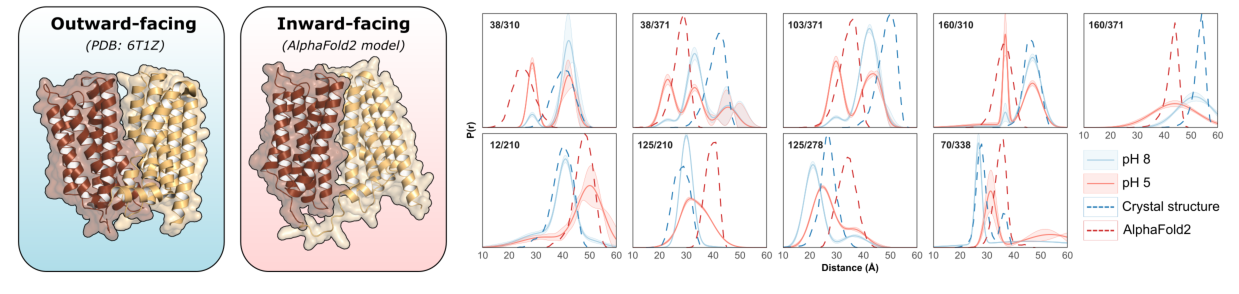
\includegraphics[width=6.5in]{Figures/lmrp_data.pdf}
 \caption[An IF model of LmrP generated by AlphaFold2 is consistent with experimental data.]{An IF model of LmrP generated by AlphaFold2 is consistent with experimental data. Left: \Gls{of} and \gls{if} conformations determined using X-ray crystallography and modeled by AlphaFold2, respectively. Right: Experimental \gls{deer} distance distributions on the extracellular and intracellular sides of the protein, respectively, overlap with distances predicted by AlphaFold2 model 1. Dashed lines are distance distributions predicted by either the crystal structure (blue) or the model (red). These data have been previously published.}
\label{fig:lmrp_data}
\end{figure}

\section{Main Text}

Active transporters such as LmrP alternate between \gls{of} and \gls{if} conformations during their transport cycles \citep*{Boudker2010, Masureel2014, Martens2016}. Whereas the crystal structure captures LmrP in the former \citep*{Debruycker2020}, AlphaFold2 modeled LmrP in the latter \citep*{Jumper2020} (Figure \ref{fig:lmrp_data}). Because LmrP is a proton/drug antiporter, we carried out \gls{deer} distance measurements \citep*{Jeschke2012, Dastvan2019, Mchaourab2011} at low and neutral pH to stabilize the \gls{if} and \gls{of} conformation, respectively (shown in red and blue in Figure \ref{fig:lmrp_data}). To evaluate the \gls{if} model's consistency with the low pH DEER data, we modeled the predicted distances \emph{in silico} using MDDS \citep*{Islam2013}, a program hosted on the CHARMM-GUI web server \citep*{Jo2014}. Not only do the predicted distances overlap remarkably well with our experimental data (Figure \ref{fig:lmrp_data}, dashed and solid lines, respectively), but importantly the magnitudes of the experimental distance changes agree with those predicted between the \gls{of} crystal structure and AlphaFold2's \gls{if} model. These results suggest that the AlphaFold2 model depicts a functionally relevant intermediate of LmrP.


\begin{wrapfigure}{r}{0.5\textwidth}
\centering
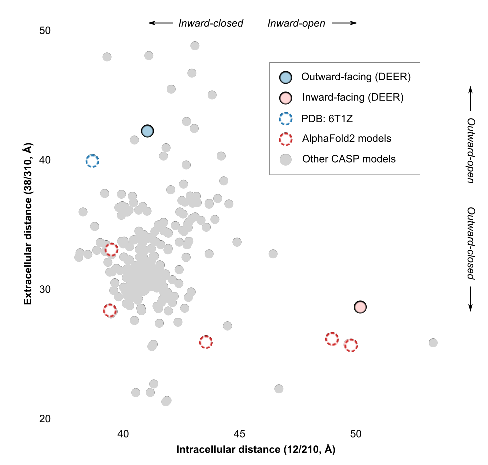
\includegraphics[width=3.25in]{Figures/lmrp_caspmodels.pdf}
 \caption[Predicted DEER distances of all CASP14 LmrP models.]{Predicted DEER distances of all CASP14 LmrP models. X and Y axes reflect the average predicted \gls{deer} distances of all \gls{casp} LmrP models on the intracellular side and extracellular sides, respectively. Solid blue and red circles represent components from the experimental \gls{deer} data corresponding to outward- and inward-facing conformations, respectively. The inward-facing AlphaFold2 model shown in panel A is located on the bottom-right.}
\label{fig:lmrp_caspmodels}
\end{wrapfigure}

The significance of this breakthrough in modeling transporter conformations is reinforced by comparison of this model to those submitted by other contestants, which overwhelmingly depicted LmrP in an occluded conformation (Figure \ref{fig:lmrp_caspmodels}). Occluded models result from methodological biases that favor compactness \citep*{Nicoludis2018}. Therefore, the success of AlphaFold2 in modeling \gls{if} LmrP suggests that these biases may finally have been overcome. Additionally, it sets the stage for the structural characterization of transporters and their functional intermediates by integrating computational modeling with experimental spectroscopy.

\section{Acknowledgments}

The work presented here was supported by the National Institutes of Health (GM077659).
\clearpage % clear the prior chapter's page

\chapter{Evaluation of scoring approaches for integrative modeling using DEER distance data} \label{app:scoring}
%\vspace{-7mm}
%\bigskip

This Appendix is based on unpublished data.

%\vspace{-7mm}
\bigskip

Conformational changes define the functional cycles of many proteins. The complete characterization of functional intermediates, such as those that are infrequently sampled or are transiently populated, continues to elude established structural biology techniques. Integrating experimental distance data collected using \gls{deer} spectroscopy with computational modeling methods promises to overcome these barriers and provide a glimpse at these states. However, experimental \gls{deer} distance distributions cannot be reliably predicted or reproduced \emph{in silico}, preventing the identification of correctly folded models to high accuracy. In part because of this fact, the scoring functions used to evaluate protein structural models using experimental DEER data in the literature vary wildly and are highly non-standard. Here we use experimental data collected in the model system PfMATE to evaluate a panel of scoring functions with the goal of determining the most effective metric for identifying correctly folded protein structures. In general, most metrics were comparable in performance when scoring unimodal distributions consistent with a single structure. However, when the data indicated a bimodal distribution representing two populations in equilibrium, only a small subset of these metrics could effectively identify native-like models. We conclude that methods comparing the overlap between the simulated and experimental distributions, rather than their average distances as is commonly performed, are more effective at identifying native-like models when structural uniformity cannot be guaranteed by the data. Nevertheless, our results indicate that optimal results can only be achieved by \emph{a priori} determination of individual conformations in the data.

\section{Introduction}

The integration of sparse experimental data collected using \gls{cryoem}, X-ray crystallography, or \gls{nmr} with Rosetta protein structure prediction allows protein models to be generated at atomic-detail accuracy \citep*{Aprahamian2019, Boura2011, Srivastava2020, Steven2008, Xia2017}. Recently, distance data collected using \gls{epr} spectroscopy in conjunction with \gls{sdsl} have been a new focus for analyzing protein structure and dynamics \citep*{Hubbell2000, Hubbell2013, Jeschke2018a, Mchaourab2011}. Even a small number of distance measurements obtained using \gls{deer} spectroscopy, which range from \SIrange{15}{80}{\angstrom}, effectively complement short-range distance data obtained using nuclear magnetic resonance spectroscopy \citep*{Ling2016, Yang2010}. As a consequence, the number of computational tools that integrate these data into modeling continues to grow \citep*{Hays2019, Hirst2011, Marinelli2019}.

The recent interest in the \gls{deer} technique has been accompanied by methodological improvements in the way the primary spectroscopic data are converted in the distance restraints for computation. A number of paradigms exist for fitting these data \citep*{Srivastava2017, Worswick2018} with model-free fitting continuing to be the most widely-used strategy \citep*{Jeschke2006, Jeschke2002}. Recent studies have identified improvements in background correction methods \citep*{FabregasIbanez2020} and have detailed the optimal balance between fitting the data and regularization \citep*{Edwards2018, FabregasIbanez2019}. By contrast, among methods that model distributions as sums of Gaussian functions, substantial work has gone into identifying more effective fitting algorithms and model selection criteria \citep*{FabregasIbanez2020a, Hustedt2018, K.IlkerSen2007, Stein2015, Sweger2020}. In both cases, these advancements have coincided with the more widespread use of confidence bands in distance distributions to visualize experimental uncertainty \citep*{Edwards2016, FabregasIbanez2020a, Hustedt2018, Sweger2020}.

Less research has been completed into determining the best approach for converting these distance data into accurate protein structural models. As a result, there is no standard approach for integrating these data for protein structural modeling. For example, it is still common to use the average or peak distance as a single restraint while disregarding the width or shape of the distance distribution \citep*{Dastvan2016, Lim2018, VanEps2018}. In other cases, distribution widths have been used as function bounds \citep*{Alexander2008, Dastvan2016a, Evans2020, Fischer2016, Ling2016}. When spin labels are explicitly modeled as flexible side chains or pseudo-rotamers, restraints have been introduced that attempt to maximize the overlap between the entire simulated and experimental distributions \citep*{Hays2019, Kazmier2014a, Marinelli2015, Raghuraman2014, Roux2013}. A functionally similar approach is to minimize the area between the integrals \citep*{Krug2016}. Finally, the primary \gls{deer} data has been used directly for model-building and refinement \citep*{Bowen2018, Hilger2007, Marinelli2019, Reichel2018}. Although direct fitting has the potential to sidestep analytical artifacts, it is unclear whether there is any quantifiable improvement in model quality as a result of using this approach. Therefore, despite the variation in these approaches, to the best of our knowledge, the optimal scoring function for protein modeling has not been determined.

Here we employ the modeling suite Rosetta to compare several different scoring approaches using the proton-coupled multidrug transporter PfMATE as a model system. Different scoring functions are found to vary substantially in their ability to identify native-like structural models using sparse \gls{deer} data. Importantly, several commonly used metrics, such as naive integration of average distance values, fail to identify native-like models when the data are multimodal, which is commonly observed in conformationally heterogeneous proteins. Using scoring functions that compute the overlap between the experimental and simulated distributions could facilitate more meaningful interpretation of protein structures from limited \gls{deer} distance data.

\section{Results and Discussion}

\subsection{Overview of the hybrid energy function}

Protein structural models are commonly evaluated using a hybrid score representing the sum of its energy and its agreement with the data. This can be written as $E_{\mathup{total}}=E_{\mathup{model}} + w_{\mathup{data}} E_{\mathup{data}}$, where $E_{\mathup{model}}$ is a model’s score derived from an energy or scoring function, $E_{\mathup{data}}$ is the function evaluating a model’s goodness-of-fit to the experimental data, and $w_{\mathup{data}}$ is the weight assigned to the experimental data relative to the native energy function \citep*{Adams1997, Jack1978}. Ideally, both $E_{\mathup{model}}$ and $E_{\mathup{data}}$ would increase monotonically as a function of a model’s deviation from the target conformation of interest. In practice, neither term alone is sufficient to unequivocally identify the experimentally determined structure of a protein. The former crudely approximates the physical forces acting upon biomacromolecules in solution, while the latter reflects agreement with measurements that may be sparse, ambiguous, and unevenly distributed. Both functions must contribute to the calculation of physiologically meaningful models.

The challenge when applying experimental \gls{deer} data as modeling constraints is the fact that the distance distributions simulated \emph{in silico} tend to overstate the dynamics of the spin label while neglecting the dynamics of the protein backbone \citep*{Hagelueken2012, Hatmal2012, Islam2013, Polyhach2011}. Any single structural model can by definition only depict a subset of the backbone conformations sampled in solution. By contrast, because clash evaluation is predominantly used to remove rotamers from structural models, the conformations of the spin labels sampled in solution are likely a subset of the rotamer libraries used to simulate these distributions. As such, it is highly unlikely that any individual structural model can exactly reproduce the experimental data.

\subsection{Overview of the benchmark}

We thus sought to determine the most effective function of $E_{\mathup{data}}$ that could most effectively identify native-like models despite these factors. Several reasons guided the choice to use the multidrug transporter PfMATE as a model system to quantify the effectiveness of various scoring methods (Table \ref{tab:scoring_metrics}). First, several crystal structures in different conformations have previously been published \citep*{Tanaka2013, Zakrzewska2019}. Second, a comprehensive panel of experimental \gls{deer} data has been previously collected and found to be largely consistent with two of these structures that face either outward (to the periplasm) or inward (to the cytoplasm) \citep*{Jagessar2020}. Third, the Rosetta suite is well equipped to model intermediate states between these two conformations. We thus generated a library of "decoy" structural models of PfMATE using Rosetta by perturbing the dihedral angles of this helix, leading to approximately 3000 alternative conformations that ranged from \gls{of} to \gls{if}, fully occluded, and fully open (see Chapter \ref{ch:multilateration} for details on how these were modeled). We then calculated the $\mathrm{C_{\upalpha}}$ \gls{rmsd} of each model to the \gls{of} state. Finally, since this conformation is sampled at neutral pH, we curated four sets of distance distributions collected at pH 7.5 that interrogated this inter-lobe distance on both the intracellular and extracellular sides of the membrane (see Table \ref{tab:pfmate_restraints} in Chapter \ref{ch:multilateration}). 



\begin{table}[b!]
\scriptsize
\renewcommand{\tabcolsep}{0.15cm}
\centering
\caption[Scoring metrics used for the benchmark.]{Scoring metrics used for the benchmark. Symbols: $\mu$: average distance; $\sigma$: standard deviation; \emph{cdf}: cumulative density function; $p_{\mathit{X}} \left( r \right)$: probability of distance $r$ in distribution $X$.}

\newcolumntype{Y}{>{\raggedright\arraybackslash}X}

\begin{center}
\begin{tabular}{l c}
\toprule \\
\textbf{Method} & \textbf{Formula} \\
\midrule \\
Average distance only & $\left( \mu_{\mathup{sim}} - \mu_{\mathup{exp}} \right)^2$ \\
Bounded range & $ max \left( 0.0, | \mu_{\mathup{sim}} - \mu_{\mathup{exp}} - \sigma | \right) $ \\
Overlap & $ \sum_{\mathup{i}=1} | p_{\mathup{sim}} \left( r_{\mathup{i}} \right) - p_{\mathup{exp}} \left( r_{\mathup{i}} \right) | $  \\
Wasserstein & $\sum_{\mathup{i}=1} |cdf_{\mathup{sim}} \left( r_{\mathup{i}} \right) - cdf_{\mathup{exp}} \left( r_{\mathup{i}} \right) | $ \\
Discrepancy & $max \left( | p_{\mathup{sim}} \left( r \right) - p_{\mathup{exp}} \left( r \right) \right) $\\
Kolmogorov-Smirnov & $max \left( | cdf_{\mathup{sim}} \left( r \right) - cdf_{\mathup{exp}} \left( r \right) \right)$ \\
Chi-squared & $\sum_{\mathup{i}=1} \frac{ \left( p_{\mathup{sim}} \left( r_{\mathup{i}} \right) \right) - p_{\mathup{exp}} \left( r_{\mathup{i}} \right)^2 }{p_{\mathup{exp}} \left( r_{\mathup{i}} \right)} $ \\
Reverse Chi-squared & $\sum_{\mathup{i}=1} \frac{ \left( p_{\mathup{exp}} \left( r_{\mathup{i}} \right) \right) - p_{\mathup{sim}} \left( r_{\mathup{i}} \right)^2 }{p_{\mathup{sim}} \left( r_{\mathup{i}} \right)} $ \\
Cross entropy & $ - \sum_{\mathup{i}=1} p_{\mathup{exp}} \left( r_{\mathup{i}} \right) \ln \left( p_{\mathup{sim}} \left( r_{\mathup{i}} \right) \right) $ \\
Jensen-Shannon distance & $ \sqrt{ \sum_{\mathup{i}=1} \left( \frac{ p_{\mathup{sim}} \left( r_{\mathup{i}} \right) } {2} \ln \left( \frac{ 2 * p_{\mathup{sim}} \left( r_{\mathup{i}} \right) } {p_{\mathup{sim}} \left( r_{\mathup{i}} \right) + p_{\mathup{exp}} \left( r_{\mathup{i}} \right)} \right) \right) + \frac{ p_{\mathup{exp}} \left( r_{\mathup{i}} \right) } {2} \ln \left( \frac{ 2 * p_{\mathup{exp}} \left( r_{\mathup{i}} \right) } {p_{\mathup{sim}} \left( r_{\mathup{i}} \right) + p_{\mathup{exp}} \left( r_{\mathup{i}} \right)} \right) } $ \\
Bhattacharyya & $- \ln \left( \sum_{\mathup{i}=1} \sqrt{ p_{\mathup{sim}} \left( r_{\mathup{i}} \right) p_{\mathup{exp}} \left( r_{\mathup{i}} \right)}  \right)$ \\
Hellinger & $1 - \sum_{\mathup{i}=1} \sqrt{ p_{\mathup{sim}} \left( r_{\mathup{i}} \right) p_{\mathup{exp}} \left( r_{\mathup{i}} \right)} $\\
Jaccard index & $\sum_{\mathup{i}=1} \frac{ min \left( p_{\mathup{sim}} \left( r_{\mathup{i}} \right), p_{\mathup{exp}} \left( r_{\mathup{i}} \right) \right) } { max \left( p_{\mathup{sim}} \left( r_{\mathup{i}} \right), p_{\mathup{exp}} \left( r_{\mathup{i}} \right) \right)}$ \\
Joint probability & $\sum_{\mathup{i}=1} p_{\mathup{sim}} \left( r_{\mathup{i}} \right) p_{\mathup{exp}} \left( r_{\mathup{i}} \right)$ \\
\bottomrule \\
\end{tabular} 
\end{center}




\label{tab:scoring_metrics}
\end{table}

In addition to evaluating the effect of each function on scoring, we also focused on the contribution of experimental noise and uncertainty to scoring. The data preparation pipeline, which is discussed in detail in \ref{sec:scoring_methods}, proceeded as follows. First, the experimental distance data at pH 7.5 were converted into raw \gls{deer} traces in the time domain with a step size of \SI{8}{ns}. Background intermolecular coupling was modeled as a stretched exponential function with background slope values ranging from $10^{-6}$ to $10^{-1}$ and modulation depth values ranging uniformly from 0.05 to 0.40, which roughly corresponds to values that would be obtained with Q-band \gls{deer} without the use of an arbitrary waveform generator.  Second, random Gaussian noise was added to these time traces to simulate the effect of \gls{snr} that were either high (noise comprises 0.5\% of the signal on average), medium (2\%), or low (10\%). Third, these data were truncated at time window durations corresponding to the number of oscillations observed, which ranged from 0.2 to 3.0 with step sizes of 0.2. Previous research suggests that at least one complete oscillation is required to accurately resolve features in the distribution beyond the mean, such as the width and multimodality. Fourth, these data were converted into distance distributions with 95\% confidence intervals in an automated fashion using the analytical software DeerLab \citep*{FabregasIbanez2020a}. Finally, to evaluate the effect of restraint quantity on scoring, between one and ten such distributions were used as restraints to evaluate each structural model of PfMATE using each of the metrics listed in Table \ref{tab:scoring_metrics}.

\subsection{Unimodal distance distribution benchmark}

The results are presented in Figure \ref{fig:scoring_heatmap}.A and show that most metrics achieve Spearman correlation coefficients of approximately 0.7 under ideal conditions (three oscillations, ten restraints, high \gls{snr}). Interestingly, experimental \gls{snr}, but not duration in the time domain, appeared to have an outsized impact on correlation quality, which may be indicative of recent advancements in background correction methods during the analysis of \gls{deer} data \citep*{FabregasIbanez2020}. The least effective metrics for model quality by Spearman correlation were the average, cross-entropy, maximum discrepancy, and Chi-squared, each of which we discuss in turn. The average distance may have been overly sensitive to long-distance components that were occasionally added when time domain data were transformed to the distance domain, but which may be absent when more deliberate data analyses are performed. Indeed, simply using a distance range appeared to ameliorate this problem. The cross-entropy metric may have been sensitive to differences in the width of the experimental and simulated distributions, since it requires perfect overlap between the domains of the two distributions (e.g., the X-axes). This may be challenging for this specific model system, as the distance data are characterized by wide distributions likely resulting from backbone disorder. The discrepancy metric captures the largest difference in amplitudes at any point in the distance distribution; given the difficulty of exactly simulating \gls{deer} distance distributions \emph{in silico}, it is unsurprising that this a poor reporter for model quality. By contrast, we are unable to rationalize why the Chi-squared metric, but not the reverse Chi-squared metric, is ineffective of distinguishing native-like from non-native-like models. None of these results were substantially affected by the inclusion of 95\% confidence intervals during calculation (data not shown).

\begin{figure}[h!]
\centering
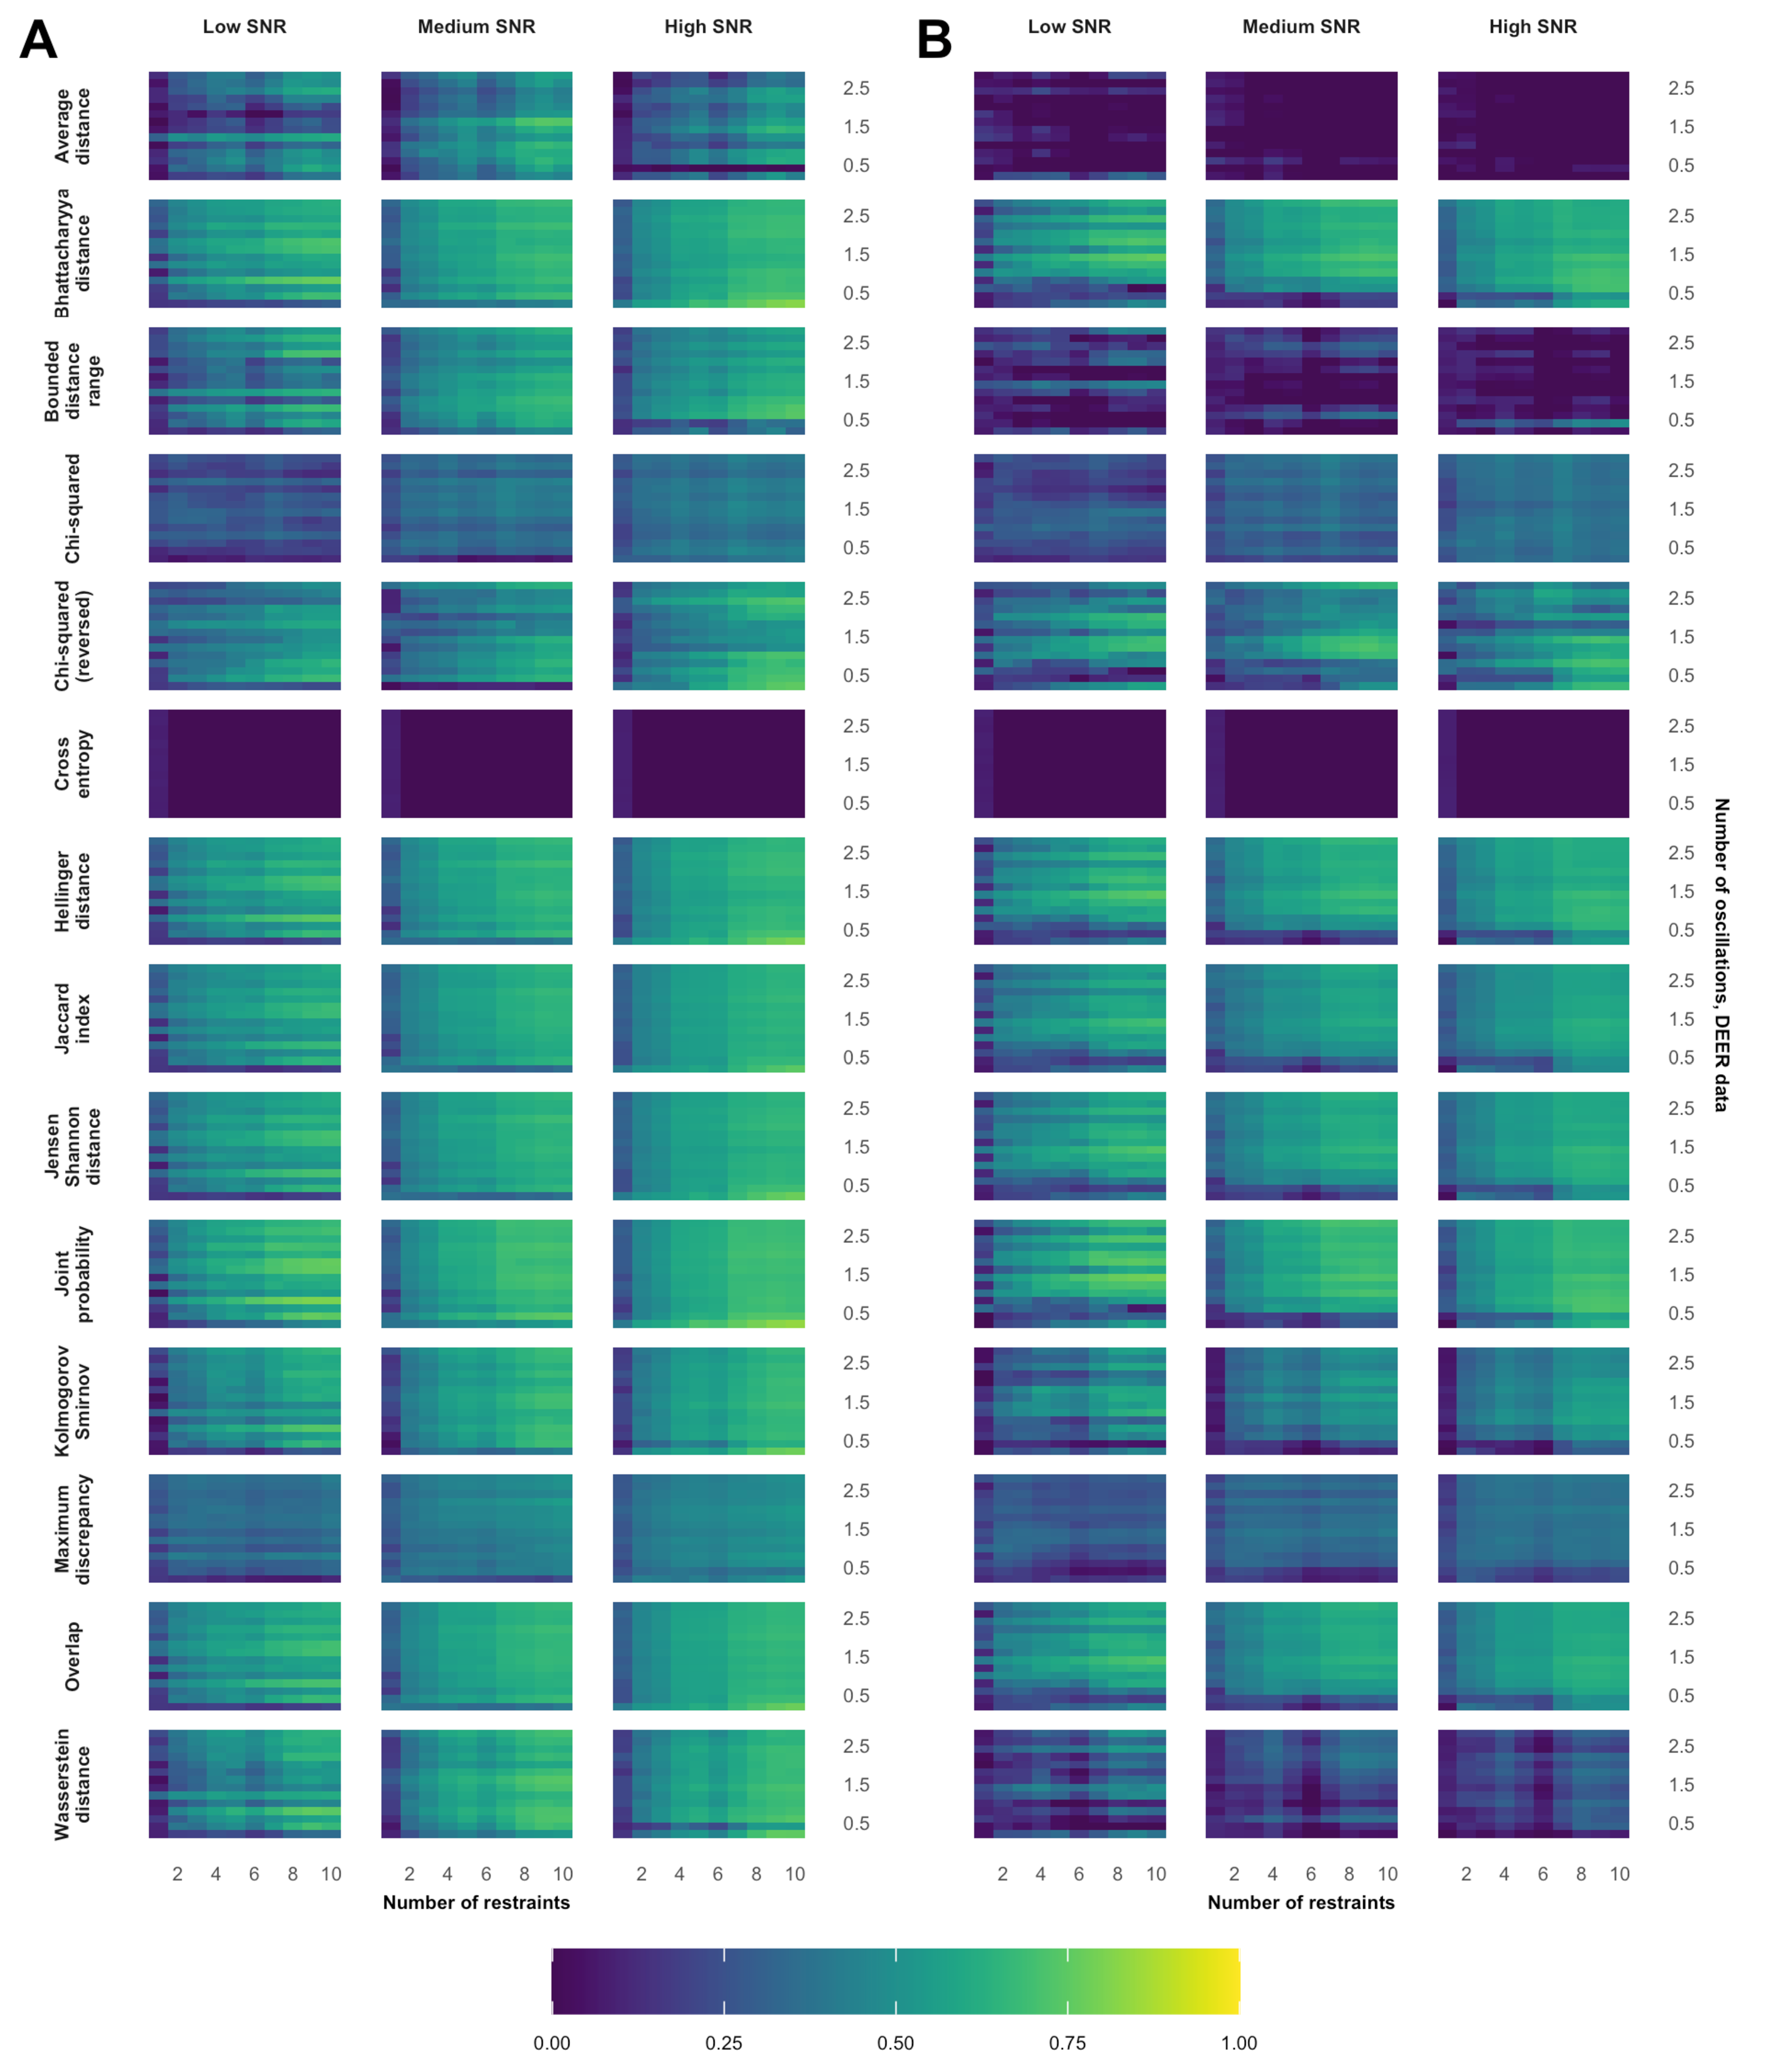
\includegraphics[width=6in]{Figures/scoring_heatmap.pdf}
 \caption[Spearman correlation coefficients between model RMSD and score as a function of number of restraints, number of oscillations in the data, and scoring function.]{Spearman correlation coefficients between model RMSD and score as a function of number of restraints, number of oscillations in the data, and scoring function. Data consist of distance distributions that are either A) unimodal or B) bimodal. Only a small number of metrics, namely those that evaluate the overlap between experimental and simulated \gls{deer} distance distributions, generate scores that correlate with \gls{rmsd} when using bimodal distributions.}
\label{fig:scoring_heatmap}
\end{figure}

\subsection{Multimodal distance distribution benchmark}

The results presented above are qualified by the fact that they were obtained using experimental data that is ideal for modeling purposes, insofar as they represent a single population or component consistent with the target crystal structure from which \gls{rmsd} values were measured. In practice, experimental data often features multiple populations with distinct distance components, some of which may be analytical artifacts or "ghost" peaks. While such data can be cleaned prior to modeling using strategies such as non-negative matrix factorization and/or global analysis \citep*{Hustedt2018, Wingler2019}, it is not always possible to exactly distinguish which distance components belong to the conformations of interest. Under circumstances where multiple components are present in the data, we would expect metrics that consider agreement with entire distributions, such as the average distance, or the Wasserstein (also called the earth mover's) distance quantifying the area between the integrals of two distributions, to be overly sensitive, and thus respond poorly, to multimodality in the data.

To test this hypothesis, we repeated the simulation pipeline outlined above, but added a distance component consistent with the \gls{if} conformation of PfMATE prior to simulation of the data in the time domain. The remaining steps of the analytical pipeline were unchanged. Each distribution in this second set of data thus consisted of an even mixture of distance components belonging to outward- and inward-facing PfMATE. The results, plotted in Figures \ref{fig:scoring_heatmap}.B and \ref{fig:scoring_comparison}, reveal that the majority of metrics considered in this study are incapable of correctly identifying models using these data, with many of their respective correlation coefficients plummeting even under ideal conditions (three oscillations, high \gls{snr}, ten restraints). Because performance was irrespective of \gls{snr} or duration in the time domain, we believe these reflect fundamental shortcomings in the ways scores are computed, rather than how the data were analyzed. We note that results obtained using these distributions, unlike the unimodal distributions discussed above, appeared to be more sensitive to time domain truncation, which may reflect the increased difficulty of resolving the shape of these distribution when there is insufficient data in the time domain.

\begin{figure}[h]
\centering
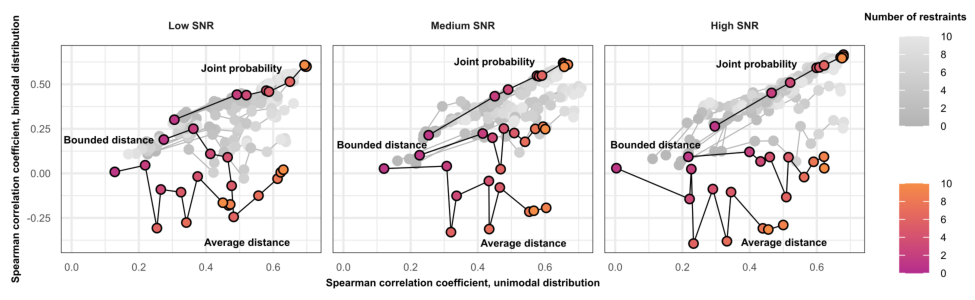
\includegraphics[width=6in]{Figures/scoring_comparison.pdf}
 \caption[Comparison of scoring methods when evaluating unimodal and bimodal distributions.]{Comparison of scoring methods when evaluating unimodal and bimodal distributions. All data used for scoring results shown here consisted of three oscillations in the time domain.}
\label{fig:scoring_comparison}
\end{figure}

Correlation coefficients calculated using several methods, such as the Jaccard index and the Joint probability, appear to be minimally affected by the presence of new components in the distance data. Interestingly, these metrics all favorably score partial overlap between distance components, while penalizing distributions that fall between the two components. This may allow specific conformations consistent with the data to be pinpointed, including the outward-open conformation from which RMSD values were calculated. It should be noted that these methods were more sensitive to time domain truncation than the unimodal distributions described above, which may demonstrate the extent to which low-quality data interferes with high-precision modeling of protein structures. Nonetheless, all of them return values that correlate slightly worse than when scoring models using unimodal distributions (Figure \ref{fig:scoring_heatmap}.A), again demonstrating the value of preprocessing the data prior to modeling.

\subsection{Concluding remarks}

This study evaluated several scoring functions using experimental \gls{deer} data in the conformationally heterogeneous model system PfMATE. We elected to use this model system, rather than a more static system such as T4 Lysozyme, due to its nonnegligible backbone dynamics that are also observed in other proteins of biophysical interest \citep*{Collauto2017, Dastvan2019, Evans2020, Martens2016, Verhalen2017a}. Indeed, while these experimental data may be broadly classified as consisting of components belonging to either outward-facing or inward-facing conformations, they also indicate substantial heterogeneity and disorder. Thus, reducing the distribution to a single value, such as an average distance, appears in this case to be detrimental to high-precision modeling. In general, the majority of scoring functions studied here return values that correlate well with model quality when the data consist of only one component. By contrast, while none of these scoring functions perfectly maintain this performance when the data consist of multiple components, a minority of these scoring functions can nonetheless return score values for models that correlate with \gls{rmsd}. Nevertheless, in all cases the Spearman correlation coefficients decreased, indicating the importance of preprocessing the data and, if possible, isolating individual components in the data prior to modeling.

\section{Materials and Methods}\label{sec:scoring_methods}

\subsection{Preparation of PfMATE decoy models}

A library of 2,855 structural models of PfMATE was generated using the software suite Rosetta 3.10 \citep*{Leaver-fay2011, Leman2020}, with both its \gls{of} (PDB: 6GWH) and \gls{if} (PDB: 6FHZ) conformations serving as template models. These models were generated using fragment insertion, in which the backbone dihedral angles of transmembrane helices 1 (residues 1-50) and 7 (residues 240-268) were perturbed using sequence fragments obtained from the Protein Databank. Sequence fragments were obtained from the Robetta web server as previously described \citep*{Kim2004}. A total of 5000 rounds of fragment insertion was executed using the scoring function \emph{score3}. Each model's structural similarity to the outward-facing state (PDB: 6GWH) was then calculated using the \emph{score\_jd2} application with residues 1-50 omitted. Finally, we binned these models by this \gls{rmsd} value and balanced the dataset to avoid the overrepresentation of models that were either fully occluded or highly inaccurate.

\subsection{Simulation and analysis of DEER data}

All experimental \gls{deer} distributions used in this study have been previously published \citep*{Jagessar2020}. Unimodal distance distributions were simulated using the data at pH 7.5 as follows. First, each distance distribution was converted into a \gls{deer} trace in the time domain with \SI{8}{ns} time steps as previously described. Each trace was normalized such that the signal intensity at \SI{0}{\upmu s} was equal to 1, and their duration was set to three oscillations, which we calculated from the average distance $r_{\mathup{avg}}$ in angstroms such that one oscillation had a duration of $ \frac{r_{\mathup{avg}}^3}{5.2*10^4} $ microseconds. Second, background coupling was simulated using the function $B \left(t \right)=\exp \left( -kt \right)$, where $k$ represents the contribution of intermolecular background coupling to the signal and $t$ is the time in microseconds. Then, normally distributed noise was added to simulate the contribution of experimental noise in the data, with the standard deviation equal to either 0.005, 0.02, or 0.1 for the high, medium, and low \gls{snr} datasets, respectively. Finally, these \gls{deer} traces were truncated to specific durations ranging from 0.2 to 3.0 oscillations and were analyzed using the \emph{fitmodel} function implemented in DeerLab v0.13.1 with default settings \citep*{FabregasIbanez2020a}.

Simulation of bimodal distributions was identical, except the experimental \gls{deer} data collected at pH 4.0 were added to the experimental distributions collected at pH 7.5 prior to transformation to the time domain.

\subsection{Scoring of PfMATE models using simulated DEER distributions}

We used the \emph{score\_jd2} application to score each PfMATE model using each of the metrics listed in Table \ref{tab:scoring_metrics}. All scoring methods were implemented in RosettaDEER. Scores were correlated with \gls{deer} values using the \emph{spearmanr} function as implemented in SciPy \citep*{Virtanen2020}.

\section{Acknowledgements}

We would like to thank Luis Fábregas Ibáñez for helpful assistance with DeerLab and Karan Bhardwaj for contributing exploratory data analysis to this study.
\clearpage % clear the prior chapter's page

\chapter{ConfChangeMover: Integrative modeling of conformational changes in LeuT-fold transporters using sparse spectroscopy data} \label{app:confchangemover}
%\vspace{-7mm}
%\bigskip

This Appendix is based on unpublished data.

%\vspace{-7mm}
\bigskip

\section{Introduction}

Active transporters, such as those with the LeuT-fold, undergo conformational changes to import and export substrates into and out of the cell \citep*{Kazmier2017}. Canonical models of symport and antiport mandate that these proteins adopt several different conformers. However, their structures are often experimentally resolved in one specific state, leaving scientists guessing at the the molecular drivers of substrate translocation. Sparse experimental data, collected using techniques such as \gls{epr} \citep*{Jeschke2012, Kazmier2014a} and/or \gls{hdxms} \citep*{Merkle2018}, can report on the structural basis of alternating access when higher-resolution methods such as \gls{cryoem} and X-ray crystallography fail. In conjunction with computational modeling, these data can provide a glimpse of the molecular details of these unknown conformers. Nonetheless, the sparseness and ambiguity of these experimental restraints make it challenging to model structures that are consistent with the data provided while retaining atomic-detail information provided by the starting X-ray or \gls{cryoem} structure.

We reasoned that the general problem surrounding the accurate modeling of conformational changes is similar in principle to that of structure refinement, in which the atomic details of structural models are deduced from low-quality models \citep*{Heo2019, Park2019, Read2019}. Recent advancements in \gls{mc} refinement methods have relied on conservative sampling described as "broken-chain kinematics" \citep*{Park2018}, in which rigid-body segments of structural models are manipulated in isolation and rejoined using loop closure (see section \ref{sec:loophash_intro} for a more detailed discussion on protein loop closure methods). This strategy has been instrumental to recent advances in homology modeling and is the foundation of widely-used methods including RosettaCM \citep*{Song2013} and Modeller \citep*{Eswar2006}. However, \gls{mc} methods are rarely employed for conformational change modeling problems, which have instead generally been tackled using either gradient minimization \cite*{Evans2020} or \gls{md} simulations \citep*{Marinelli2019, Sfriso2016}. Both methods are computationally expensive and can potentially understate the extent to which protein backbones reconfigure. 

Here we describe a general-purpose \gls{mc} sampling method, ConfChangeMover, which we implemented in the macromolecular modeling program Rosetta \citep*{Leaver-fay2011, Leman2020} and designed to model conformational changes using sparse experimental data (Figure \ref{fig:ccm_scheme}). The method combines recent conceptual advances borrowed from cutting-edge homology modeling methods with novel sampling approaches designed to conservatively manipulate a starting structure. Whereas homology modeling is concerned with identifying the dihedral angles of a protein that satisfy spatial restraints provided by one or more template models, our approach instead samples spatial rearrangements consistent with dihedral angles observed in the starting structure. We first demonstrate ConfChangeMover on a panel of soluble proteins using simulated $\mathrm{C_{\upalpha}}$-$\mathrm{C_{\upalpha}}$ distance restraints. Then, using experimental \gls{epr} data that has been previously published, we apply the method to three transporters with the LeuT-fold fold (described in detail in Chapter \ref{ch:leutintro}).


\begin{figure}[h]
\centering
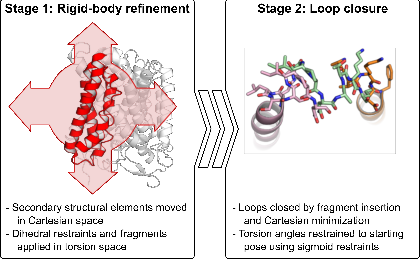
\includegraphics[width=5in]{Figures/ccm_scheme.pdf}
 \caption[Overview of the ConfChangeMover sampler.]{Overview of the ConfChangeMover sampler.}
\label{fig:ccm_scheme}
\end{figure}


\section{Materials and Methods}

\subsection{Overview of the sampling approach}


ConfChangeMover was implemented in Rosetta and executed in RosettaScripts \citep*{Fleishman2011}. As with RosettaCM, it samples candidate structural models using a two-stage strategy (Figure \ref{fig:ccm_scheme}). Prior to the first stage, the input structure is converted to a coarse-grained model with side chains replaced by immobile centroid pseudo-atoms. Cutpoints are introduced at residues located on loops connecting pairs of rigid bodies, or segments, which consist of either $\mathrm{\upalpha}$-helices or $\mathrm{\upbeta}$-sheets identified using the \gls{dssp} \citep*{Kabsch1983}. These cutpoints allow the positions and conformations of these segments to be perturbed either in isolation or in concert in the first stage without downstream propagation to rest of the protein via the "lever-arm effect" \citep*{Tyka2012}. A series of sigmoid dihedral constraints, discussed below in section \ref{sec:confchangemover_restraints}, are added to model.

During the first stage, several types of perturbations are randomly introduced in the structural model. These include:

\begin{itemize}
    \item \textbf{Rigid-body movements of one \gls{sse}.} Rotation angles and translation vectors are randomly drawn from normal distributions with standard deviations of 15° and \SI{2.0}{\angstrom}, respectively.
    \item \textbf{Rigid-body movements of multiple spatially adjacent \gls{sse}s.} The number of \gls{sse}s randomly ranges from 2 to $N-1$, where $N$ is the number of segments in the model, and the movement parameters match those used for a single \gls{sse}.
    \item \textbf{Helical twists.} Helices are twisted by a randomly chosen angle drawn from a normal distribution with a standard deviation of 15°.
    \item \textbf{Fragment insertion.} The dihedral angles of a three-residue stretch of the protein are modified to match those of a randomly chosen sequence fragment obtained from the PDB. Fragments were obtained using the Robetta web server as previously described \citep*{Kim2004}.
\end{itemize}

Throughout this stage, \gls{sse}s that are adjacent in sequence are constrained such that their N- and C-terminal ends can be plausibly bridged by the loop connecting them. We achieved this by automatically rejecting moves that separate the termini of consecutive \gls{sse}s by distances greater than $2.65n_{\mathup{res}}+2.11$ \AA, where $n_{\mathup{res}}$ is the number of residues in the loop \citep*{Woetzel2012}.

During the second stage, loops are closed using a method similar to one described previously \citep*{Rohl2004} that is used by RosettaCM \citep*{Song2013}. However, ConfChangeMover supplements this procedure using stretches of the starting model ranging from three to fifteen residues in length. The perturbations available include:

\begin{itemize}
    \item \textbf{Fragment superimposition over gap regions.} Nine-residue fragments obtained from the PDB are superimposed over unresolved gaps in the structure.
    \item \textbf{Fragment superimposition over randomly chosen regions.} Nine-residue fragments are superimposed over randomly-chosen regions, which can include those that do not contain chainbreaks.
    \item \textbf{Template superimposition.} Stretches of residues with lengths ranging from nine to fifteen residues are copied from the starting conformation and superimposed over the model.
\end{itemize}

As with RosettaCM, during the final 25\% of the second stage, each move is followed by a brief Cartesian minimization \citep*{Conway2014} using the limited-memory Broyden-Fletcher-Goldfarb-Shanno algorithm \citep*{Byrd1995}. At the end of stage 2, the entire model is minimized using the same approach.

During an optional third stage, all-atom side chains replace the centroid pseudo-atoms, and the entire model is iteratively minimized as previously described \citep*{Conway2014, Song2013}.

\subsection{Application of constraints during modeling}\label{sec:confchangemover_restraints}

Several types of constraints are applied to these models throughout the algorithm. To account for the relative invariance of protein dihedral angles during conformational change modeling (see section \ref{sec:ccm_results_dihedrals}), circular sigmoidal restraints are added to the $\phi$ and $\psi$ angles of the model based on either the starting conformation or a separate model provided by the user:

\begin{equation}
    S_{\upphi}(x) = \left( 1 + \exp \left( | \phi_{\mathup{sim}} - \phi_{\mathup{exp}} | - \frac{\pi}{2} \right) \right)^{-1} + \left( 1 + \exp \left( | \phi_{\mathup{sim}} - \phi_{\mathup{exp}} | + \frac{\pi}{2} \right) \right)^{-1}
\end{equation}

\begin{equation}
    S_{\uppsi}(x) = \left( 1 + \exp \left( | \psi_{\mathup{sim}} - \psi_{\mathup{exp}} | - \frac{\pi}{2} \right) \right)^{-1} + \left( 1 + \exp \left( | \psi_{\mathup{sim}} - \psi_{\mathup{exp}} | + \frac{\pi}{2} \right) \right)^{-1}
\end{equation}

Additionally, following stage 1, coordinate constraints were applied to the $\mathrm{C_{\upalpha}}$ atoms of all residues belonging to \gls{sse}s. This allowed fragment insertions during stage 2 to close loops while minimally affecting the dihedral angles obtained following stage 1.

\subsection{Benchmark on soluble proteins using simulated distance restraints}

We first tested ConfChangeMover on seven soluble proteins (Table \ref{tab:ccm_proteins}). These topologically dissimilar proteins were selected from previous benchmarks \citep*{Jeschke2012, Sfriso2016}. We first modeled all missing residues using RosettaCM \citep*{Song2013}. Distance restraints between $\mathrm{C_{\upalpha}}$ atoms were selected from the starting structure using a modification of the Zheng-Brooks algorithm as implemented in the program MMM \citep*{Jeschke2012, Jeschke2018a, Polyhach2011, Zheng2005}, with one restraint per twenty residues in the total protein sequence, rounding up. For the benchmark on soluble proteins, we compared ConfChangeMover to fragment insertion, in which the dihedral angles of the starting structures were directly modified. For both methods, regions that did not undergo conformational transitions between the two states were not permitted to move and were not used for \gls{rmsd} calculations.

\begin{table}[h]
\scriptsize
\renewcommand{\tabcolsep}{0.09cm}
\centering
\caption[Protein structures used in the benchmark of ConfChangeMover.]{Protein structures used in the benchmark of ConfChangeMover. $^{\dagger}$ A model of \gls{of} vSGLT was generated from the X-ray structure of the homolog SiaT. This model was not used as a target model in this benchmark. $^{\ddagger}$ Insufficient experimental restraints were available to model the \gls{of}-to-\gls{if} transition in LeuT.}

%\newcolumntype{Y}{>{\raggedright\arraybackslash}X}

% Structures are marked if they were mutated ($\dagger$) or bound to inhibitors ($\ddagger$) or antibodies ($\mathsection$).}

\begin{center}
\begin{tabular}{l l l l r}
\toprule \\
\textbf{Protein \emph{(Organism)}} & \textbf{PDB A (Resolution)} & \textbf{PDB B (Resolution)} & \textbf{Length} & \textbf{References} \\
\midrule \\
\multicolumn{5}{l}{\textbf{Soluble proteins (simulated data)}} \\
Adenosylcobinamide kinase (\emph{Salmonella enterica}) & 1CBU (\SI{2.30}{\angstrom}) & 1C9K (\SI{2.20}{\angstrom}) & 181 & \citep*{Thompson1998, Thompson1998a} \\
DNA polymerase I (\emph{Thermophilus aquaticus}) &  2KTQ (\SI{2.30}{\angstrom}) & 3KTQ (\SI{2.30}{\angstrom}) & 832 & \citep*{Li1998} \\
Glutamine-binding protein (\emph{Escherichia coli}) & 1GGG (\SI{2.30}{\angstrom}) & 1WDN (\SI{1.94}{\angstrom}) & 248 & \citep*{Hsaio1996, Sun1998} \\
Lactoferrin (\emph{Homo sapiens}) & 1LFH (\SI{2.80}{\angstrom}) & 1LFG (\SI{2.20}{\angstrom}) & 710 & \citep*{Haridas1995, Norris1991} \\
Leucine-binding protein (\emph{E. coli}) & 1USI (\SI{1.80}{\angstrom}) & 1USG (\SI{1.53}{\angstrom}) & 369 & \citep*{Magnusson2004} \\
Mitochondrial aspartate aminotransferase (\emph{Gallus gallus}) & 1AMA (\SI{2.30}{\angstrom}) & 9AAT (\SI{2.20}{\angstrom}) & 423 & \citep*{McPhalen1992, McPhalen1992a} \\
Pol alpha DNA polymerase (\emph{Escherichia} phage RB69) & 1IG9 (\SI{2.60}{\angstrom}) & 1IH7 (\SI{2.21}{\angstrom}) & 903 & \citep*{Franklin2001} \\
\\
\multicolumn{5}{l}{\textbf{LeuT-fold proteins (experimental data)}} \\
LeuT (\emph{Aquifex aeolicus}) & 2A65 (\SI{1.65}{\angstrom}) & $\mathrm{3TT3}^\ddagger$ (\SI{3.22}{\angstrom}) & 513 & \citep*{Krishnamurthy2012, Yamashita2005} \\
Mhp1 (\emph{Microbacterium tumefaciens}) & 2JLN (\SI{2.85}{\angstrom}) & 2X79 (\SI{3.80}{\angstrom}) & 489 & \citep*{Shimamura2010, Weyand2008} \\
vSGLT (\emph{Vibrio parahaemolyticus}) & 2XQ2 (\SI{2.73}{\angstrom}) & $\mathrm{5NV9^\dagger}$ (\SI{1.95}{\angstrom}) & 543 & \citep*{Wahlgren2018, Watanabe2010} \\
\bottomrule \\
\end{tabular} 
\end{center}
\label{tab:ccm_proteins}
\end{table}

\subsection{Benchmark on LeuT-fold transporters proteins using experimental EPR restraints}

For the benchmark using experimental data, ConfChangeMover was tested using three LeuT-fold transporter proteins: LeuT \citep*{Krishnamurthy2012, Yamashita2005}, Mhp1 \citep*{Shimamura2010, Weyand2008}, and vSGLT \citep*{Watanabe2010} (Table \ref{tab:ccm_proteins}). These three proteins have previously been studied using \gls{epr}, and all undergo ligand-dependent conformational transitions between \gls{if} and \gls{of} conformations \citep*{Claxton2010, Kazmier2014, Kazmier2014a, Paz2018}.

Four transitions of interest were used to benchmark ConfChangeMover (Table \ref{tab:ccm_proteins}). In each case, experimental data was provided using the RosettaDEER module (see Chapter \ref{ch:rosettadeer}). For LeuT, the \gls{if}-to-\gls{of} transition took advantage of distance restraints collected on LeuT in the presence of the detergent $\mathrm{\upbeta}$-OG \citep*{Kazmier2014a}. In Mhp1, the \gls{of}-to-\gls{if} and \gls{if}-to-\gls{of} transitions were simulated using \gls{deer} data collected either without substrates or with both sodium and benzylhydantoin, respectively \citep*{Kazmier2014}. Finally, because vSGLT has only been crystallized in \gls{if} conformations \citep*{Faham2008, Watanabe2010}, we modeled the \gls{of}-to-\gls{if} transition by starting from a previously published \gls{of} homology model generated from the homologous sialic acid transporter SiaT \citep*{Paz2018, Wahlgren2018}. The \gls{if}-to-\gls{of} transition of vSGLT and the \gls{of}-to-\gls{if} transition of LeuT were not modeled.

For both benchmarks, we set stages 1 and 2 to consist of 50,000 rounds and 1,000 rounds, respectively. The weights of the score terms \emph{dihedral\_constraint}, \emph{atompair\_constraint}, and \emph{coordinate\_constraint} were set to 1.0, 10.0, and 1.0, respectively. The Rosetta scoring functions \emph{score3} and \emph{score4\_smooth\_cart} were used for stages 1 and 2, respectively. We generated 100 models using each method for the soluble protein benchmark and 1000 models for the LeuT-fold benchmark. 

\section{Results and Discussion}

\subsection{Most dihedral angles do not change during conformational isomerization}\label{sec:ccm_results_dihedrals}

To determine the extent to which dihedral $\phi$ and $\psi$ angles rotate during conformational change, we compared pairs of structures from a panel of conformational changes used in a recent benchmark \citep*{Jeschke2012a}. Comparison of proteins in multiple states revealed that the overwhelming majority of backbone dihedral angles in proteins remain unchanged when undergoing conformational transitions, suggesting that interconversion between two states may be facilitated by a small fraction of residues as previously suggested \citep*{Sauer2020} (Figure \ref{fig:ccm_angles}). This expectation was implemented as a modeling restraint using circular sigmoidal functions on the backbone $\phi$ and $\psi$ angles (see section \ref{sec:confchangemover_restraints}). Sigmoidal restraints have previously been used for modeling proteins using restraints with a small number of false positives, such as those obtained using residue coevolution \citep*{Ovchinnikov2015, Ovchinnikov2017, Teixeira2017}, because they favor structural models that satisfy as many restraints as possible while minimizing the contribution of noisy data to the resulting model. 

\begin{figure}[h]
\centering
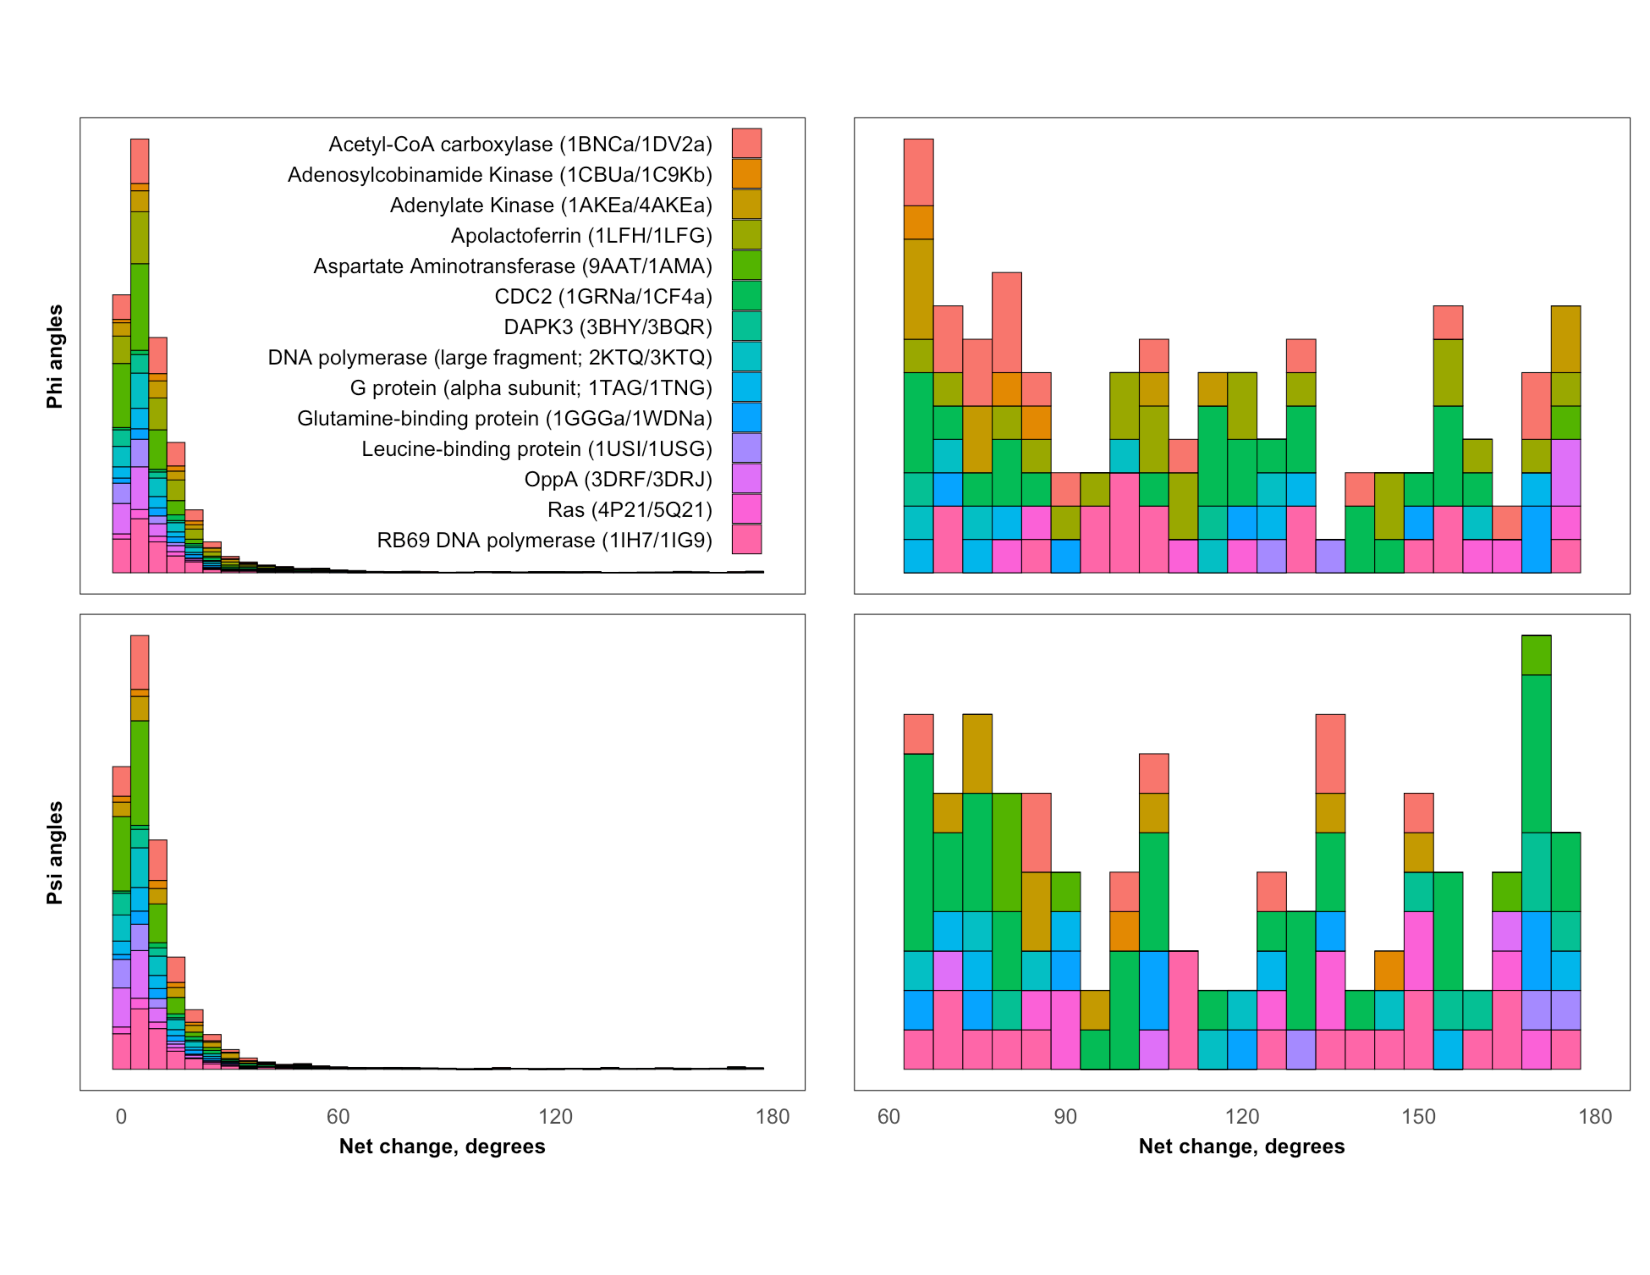
\includegraphics[width=6.5in]{Figures/ccm_angles.pdf}
 \caption[Rotational changes observed in the dihedral angles of various proteins undergoing conformational changes.]{Rotational changes observed in the dihedral angles observed in various proteins undergoing conformational changes. Left: the overwhelming majority of dihedral angles in the dataset rotate less than 30° during isomerization. Right: Close-up of cases that rotate more than 60°.}
\label{fig:ccm_angles}
\end{figure}

\subsection{Benchmark on soluble proteins}

We first benchmarked ConfChangeMover on a panel of seven soluble proteins using simulated distance restraints (Table \ref{tab:ccm_proteins}). Both directions were used as part of the benchmark, leading to fourteen total transitions. These proteins were specifically chosen for their complex modes of conformational isomerization, wherein loops and \gls{sse}s moves in ways that are unlikely to be easily recapitulated by simple rotation of backbone dihedral angles \citep*{Dastvan2016a, Krug2016}. To test that this was the case, the performance of ConfChangeMover was compared to simple fragment insertion. For both methods, regions that do not move in between these two states were not manipulated. Distance restraints between $\mathrm{C_{\upalpha}}$ atoms were chosen using a previously published restraint-picking algorithm \citep*{Jeschke2012a, Zheng2005} and simulated from the target structure. Following the simulation, $\mathrm{C_{\upalpha}}$ \gls{rmsd} values were calculated exclusively from the mobile regions of the protein.

The results are plotted in Figure \ref{fig:ccm_soluble}. In the absence of restraints, the majority of models sampled using ConfChangeMover were nearly identical to the starting model, indicated by the dashed line, suggesting that the starting structure generally occupied an energy minimum that may be difficult to escape. Introducing simulated $\mathrm{C_{\upalpha}}$-$\mathrm{C_{\upalpha}}$ restraints led to improvements in \gls{rmsd} in every protein except lactoferrin.  In contrast, using restraints with fragment insertion generally led to unfolding of the models and worsening of \gls{rmsd} relative to the starting structure (see Figure \ref{fig:ccm_soluble}.A), despite the fact that fragments were only inserted in stretches of mobile residues. In general, the breadth of models sampled this way was both far larger and universally poorer in quality than those obtained ConfChangeMover. The exception to this second point, lactoferrin, appeared to be modeled relatively easily by simple changes in the dihedral angles connecting two domains. Additionally, the majority of simulated restraints obtained using the modified Zheng-Brookes restraint-picking algorithm discussed above did not cover mobile portions of the protein. As a result, we believe the aggressive sampling available to fragment insertion may have been beneficial to escaping the local minimum and sampling conformers similar to the target. Nevertheless, the majority of models did worsen in \gls{rmsd} relative to the starting structure.

\begin{figure}[h!]
\centering
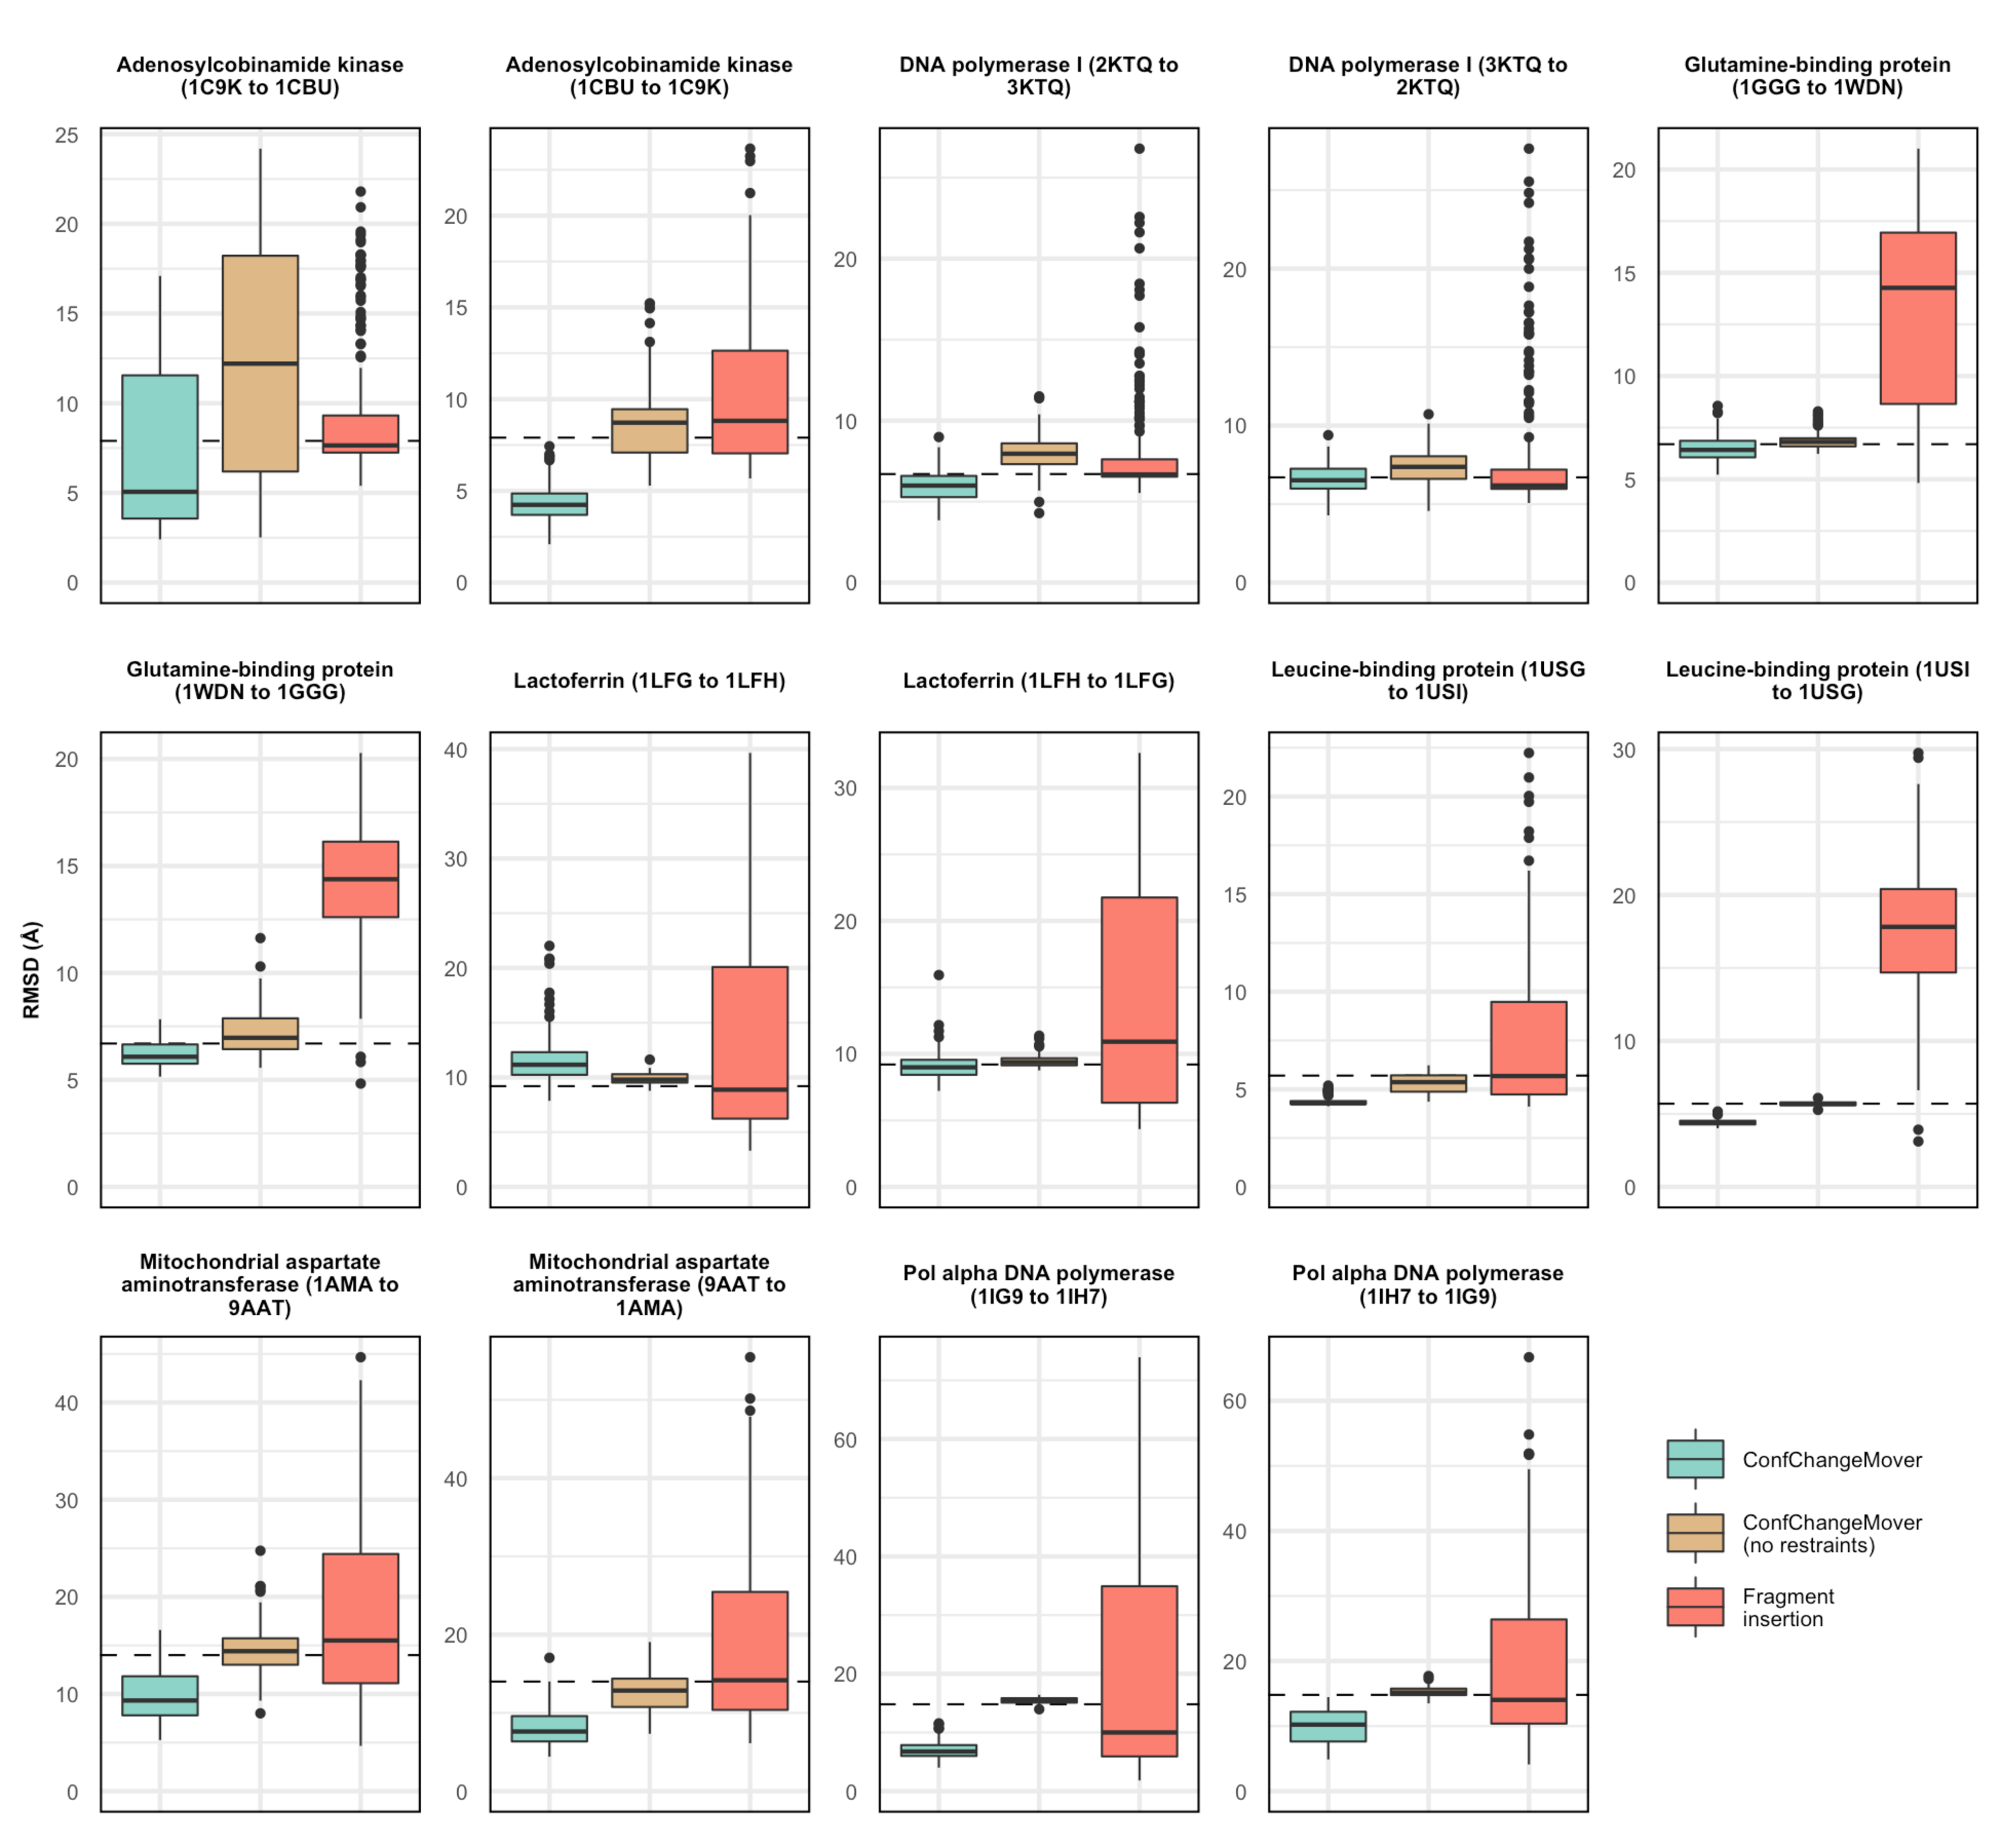
\includegraphics[width=6.5in]{Figures/ccm_soluble.pdf}
 \caption[ConfChangeMover outperforms fragment insertion in Rosetta when modeling conformational changes in soluble proteins using simulated $\mathrm{C_{\upalpha}}$ restraints.]{ConfChangeMover outperforms fragment insertion in Rosetta when modeling conformational changes in soluble proteins using simulated $\mathrm{C_{\upalpha}}$ restraints. Starting models indicated by the dashed black line. }
\label{fig:ccm_soluble}
\end{figure}

The remaining proteins in the benchmark set generally show a consistent pattern in which sampling using ConfChangeMover is focused and worsening of models is generally avoided. This is the principal challenge of structure refinement \citep*{Park2018}, as there are many more ways to ruin a structural model than improve it.

\subsection{Benchmark on LeuT-fold transporters using experimental data}

With these results in hand, we then applied this method to LeuT-fold transporters that have been experimentally studied using \gls{epr}. The transmembrane domains of these transporters are entirely $\mathrm{\upalpha}$-helical and undergo various divergent modes of isomerization to facilitate translocation of substrates across the membrane (see Chapter \ref{ch:leutintro} for details). Libraries of \gls{deer} measurements collected in LeuT, Mhp1, and vSGLT are generally consistent with experimental structures. For LeuT, due to outstanding controversies surrounding the conformational details of the \gls{if} state \citep*{Kazmier2014a, Sohail2016}, we exclusively simulated the \gls{if}-to-\gls{of} transition using experimental measurements collected in the detergent \gls{bog}. Helices in the bundle domain, as well as \gls{tmh}5 and \gls{el}4, were permitted to move, while the positions of the hash domain and \gls{tmh}10-12 were fixed. For Mhp1, both the \gls{if} and \gls{of} conformations were largely found to be consistent with \gls{epr} data collected in the apo and substrate-bound state and indicated rigid-body movement of the hash domain and bending of \gls{tmh}5. For vSGLT, which has only been crystallized in \gls{if} conformations, we modeled the \gls{of}-to-\gls{if} conformational change starting from an \gls{of} homology model generated from the structure of the homolog SiaT \citep*{Wahlgren2018} that was generated for a previous study \citep*{Paz2018}. The conformational changes suggested by the \gls{epr} data are largely consistent with those expected from this model and suggest a mechanism of alternating access that combines elements of both LeuT and Mhp1 that involve helices across the whole protein. We repeated the conformational change modeling procedure and compared it to both fragment insertion and to the homology modeling program RosettaCM \citep*{Song2013}. Additionally, to evaluate the impact of experimental restraints on modeling, ConfChangeMover was also run with simulated \gls{deer} restraints generated using MDDS \citep*{Islam2013}, as well as simulated $\mathrm{C_{\upalpha}}$-$\mathrm{C_{\upalpha}}$ distance restraints generated from the target model.


\begin{figure}[h!]
\centering
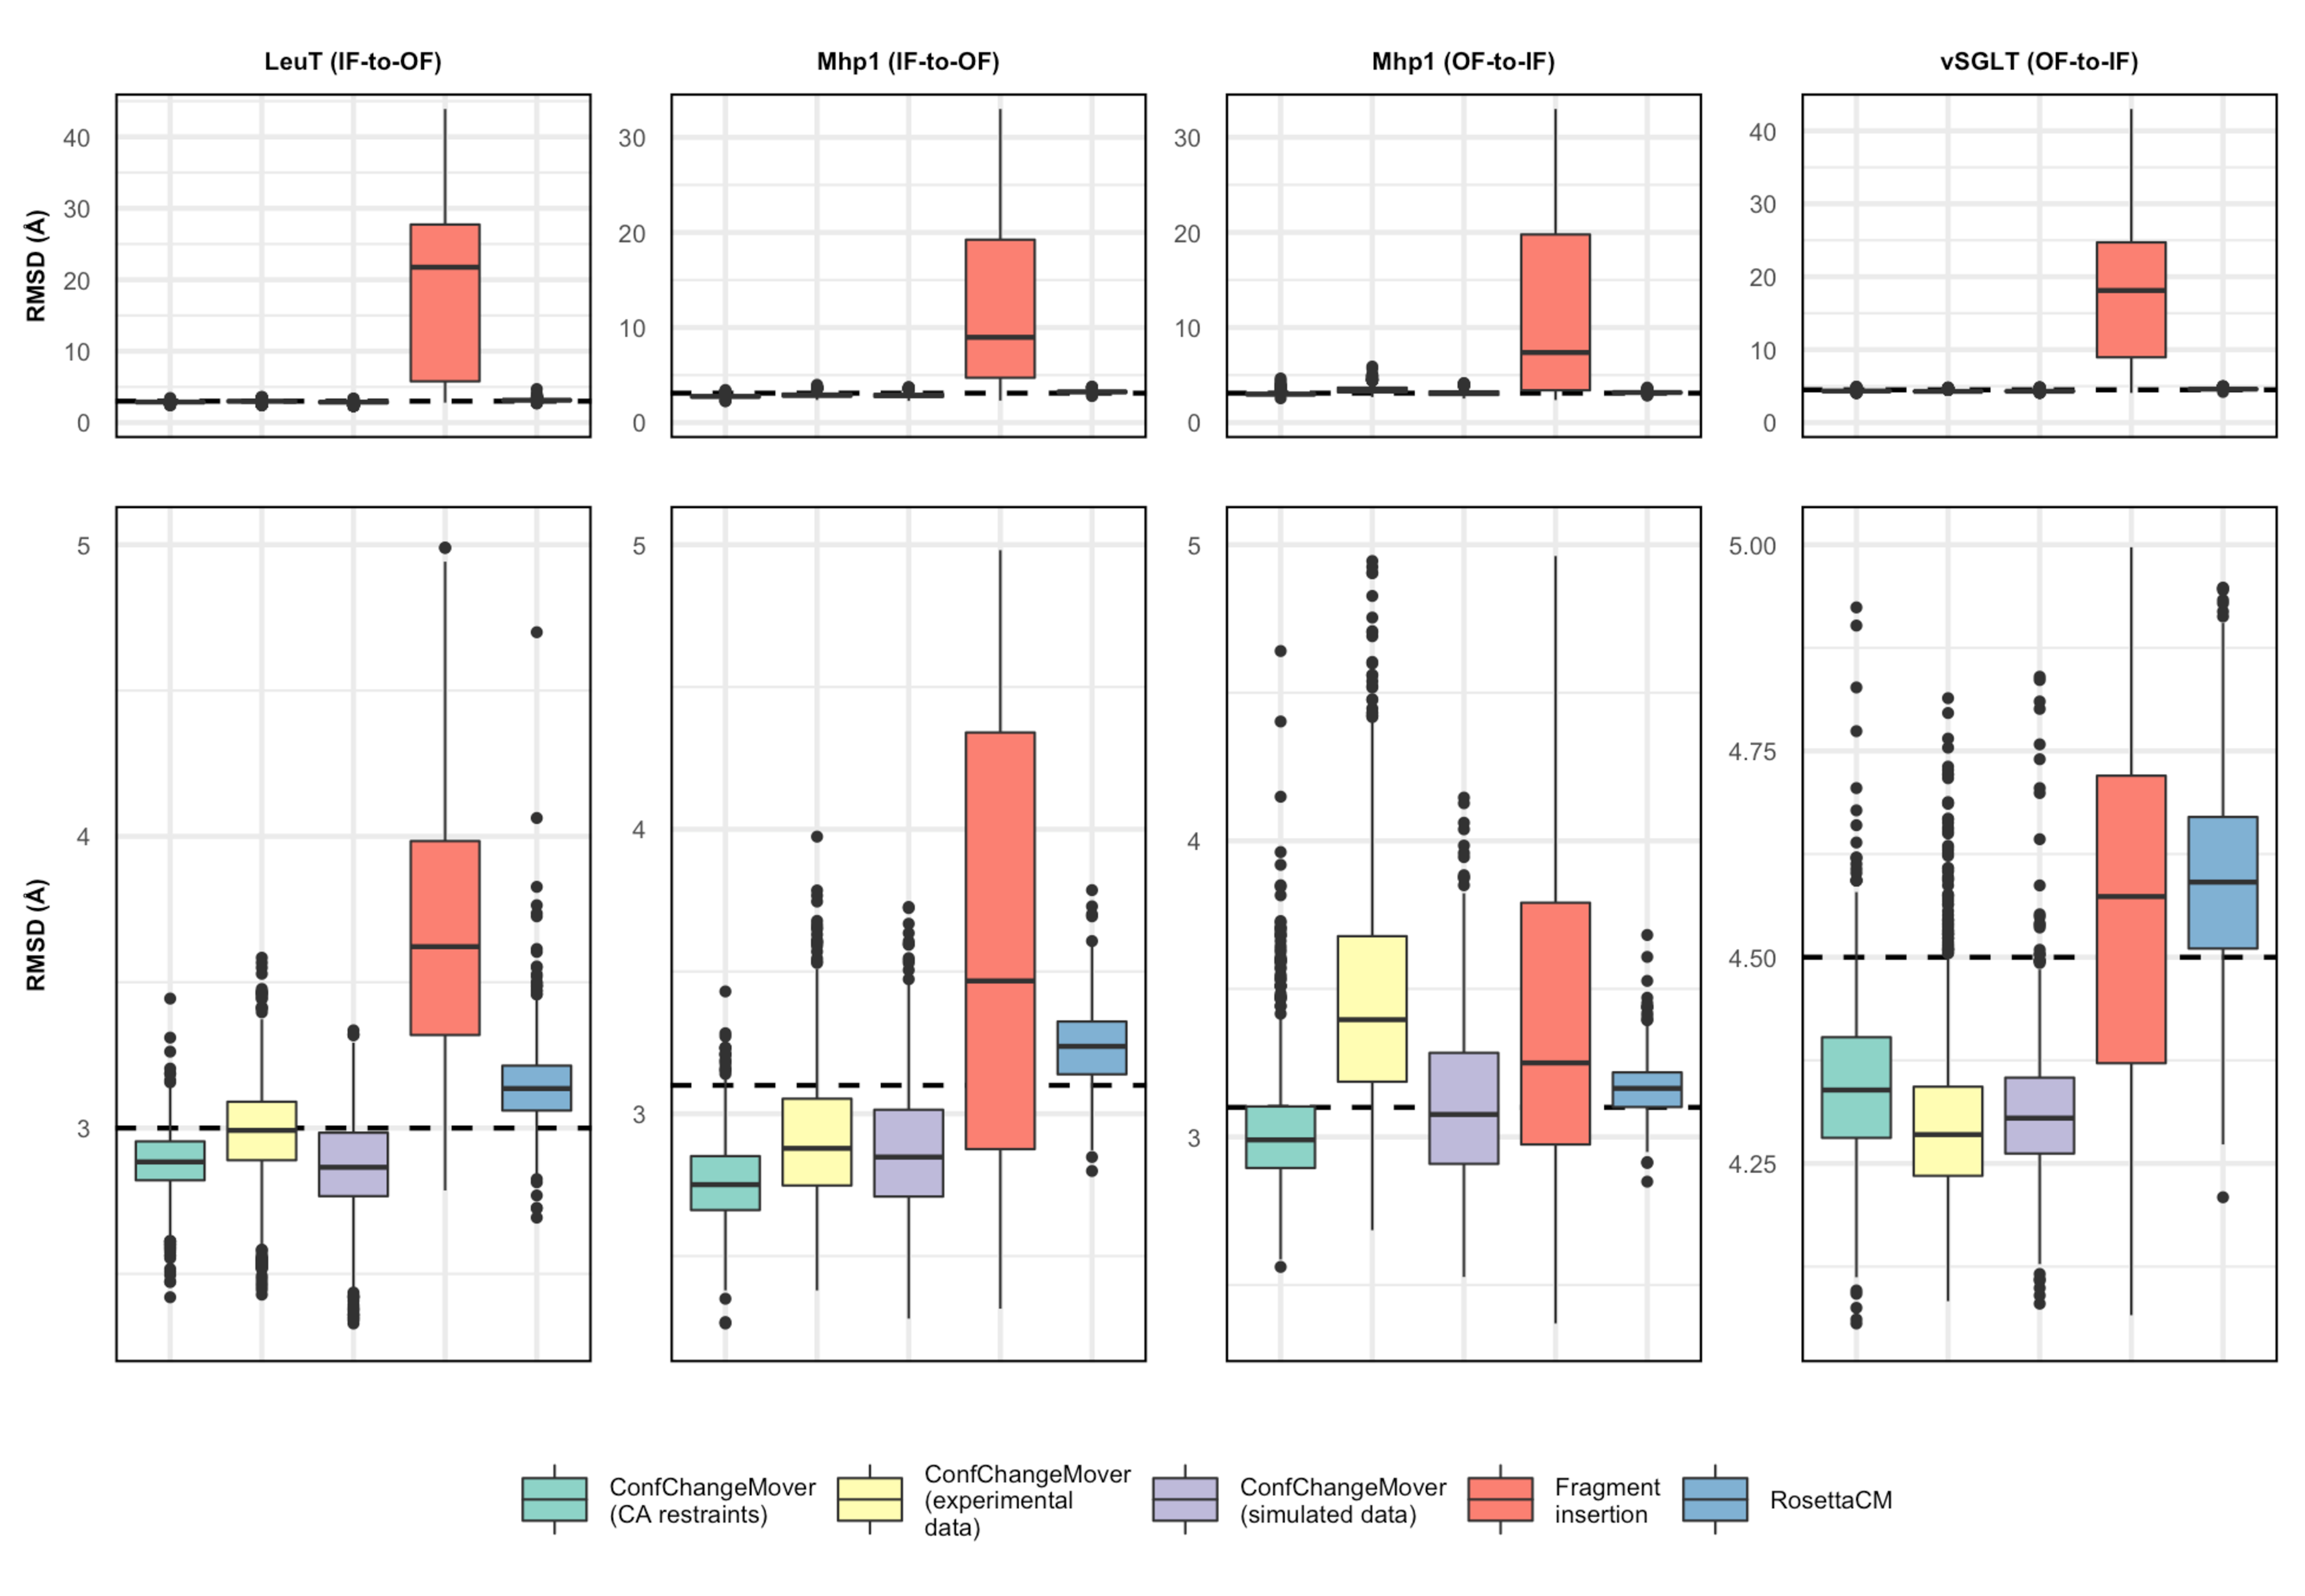
\includegraphics[width=6.5in]{Figures/ccm_leut.pdf}
 \caption[ConfChangeMover outperforms available methods in Rosetta when modeling conformational changes in LeuT-fold transporters using EPR data.]{ConfChangeMover outperforms available methods in Rosetta when modeling conformational changes in LeuT-fold transporters using EPR data. Starting models indicated by the dashed black line.}
\label{fig:ccm_leut}
\end{figure}

The results are shown in Figure \ref{fig:ccm_leut} and repeat the pattern observed in those obtained in the soluble protein benchmark. ConfChangeMover largely samples structures similar to the starting model, with virtually all models improving in \gls{rmsd} relative to the starting structure. The exception, \gls{of}-to-\gls{if} Mhp1, saw most models get worse in quality. The striking different between models generated using simulated and experimental data suggested that poor model quality could be attributed to differences between predicted and experimental spin label distances. Indeed, a distance restraint between \gls{tmh}1a and \gls{tmh}9 on the intracellular side of the protein (30/338) differed from predictions obtained using MDDS by \SI{14}{\angstrom} \citep*{Kazmier2014}. Additionally, visual examination of representative models obtained using simulated \gls{deer} restraints revealed that the kinked \gls{tmh}5 facilitating substrate egress into the cytoplasm could not be recapitulated using this method (Figure \ref{fig:ccm_bestmodels}). 

Related to this observation, we found that in three cases the $\mathrm{C_{\upalpha}}$-$\mathrm{C_{\upalpha}}$ distance restraints provided the greatest benefit, suggesting that the precision obtained when directly restraining the backbone is generally superior to those obtained from spin probes measured using \gls{deer}. The results from the fourth case, vSGLT, were not statistically different from either experimental or simulated \gls{deer} data (unpaired two-tailed $t$-test), highlighting the consistency of that crystal structure with the experimental \gls{deer} data.

\begin{figure}[h!]
\centering
\includegraphics[width=6.5in]{Figures/ccm_bestmodels.pdf}
 \caption[Lowest RMSD models obtained using ConfChangeMover with experimental EPR restraints.]{Lowest RMSD models obtained using ConfChangeMover with experimental EPR restraints.}
\label{fig:ccm_bestmodels}
\end{figure}

In marked contrast, and as was seen in the soluble protein benchmark, we found that fragment insertion similarly unfolded these models, with average \gls{rmsd} values of \SIrange{10}{25}{\angstrom} (Figure \ref{fig:ccm_soluble}). Unlike the soluble protein benchmark, in no cases did it outperform ConfChangeMover among proteins with this topology. Additionally, the homology modeling program RosettaCM sampled too conservatively and did not allow models to be modified away from the starting structure.

\subsection{Concluding remarks}

The modeling protocol ConfChangeMover is presented and discussed. Benchmarks in both soluble proteins using simulated distance restraints and membrane transporter proteins using experimental restraints show how this method can tackle various modes of conformational interconversion while generating models that nonetheless resemble the starting conformation. Its implementation as a Mover in Rosetta allows it to be used in combination with countless other modeling methods. Further development should focus on combining ConfChangeMover with other protocols, or embedding it in more complex modeling approaches \citep*{Park2018}.

\subsection{Acknowledgements}

We would like to thank Dr. Davide Sala for collaborating on this project and Dr. Marion F. Sauer for fruitful discussions during its early stages. The research in this Appendix was supported by the National Institutes of Health (R01 GM080403 and R01 GM073151), and by the Deutsche Forschungsgemeinschaft (DFG, German Research Foundation) through SFB1423, project number 421152132, subproject A07 and Z04. 
\clearpage % clear the prior chapter's page

\chapter{Efficient sampling of loop conformations using conformational hashing and random coordinate descent} \label{app:loophash}
%\vspace{-7mm}
%\bigskip

The contents of this Appendix have been previously published \citep*{DelAlamo2021}.

%\vspace{-7mm}
\bigskip

\emph{De novo} construction of loop regions is an important problem in computational structural biology. Compared to regions with well-defined secondary structure, loops tend to exhibit significant conformational heterogeneity. As a result, their structures are often ambiguous when determined using experimental data obtained by crystallography, \gls{cryoem}, or \gls{nmr}. Although structurally diverse models could provide a more relevant representation of proteins in their native states, obtaining large numbers of biophysically realistic and physiologically relevant loop conformations is a resource-consuming task. To address this need, we developed a novel loop construction algorithm, Hash/RCD, that combines knowledge-based conformational hashing with \gls{rcd}. This hybrid approach achieved a closure rate of 100\% on a benchmark set of 195 loops in 29 proteins that range from three to thirty-one residues. More importantly, the use of templates allows Hash/RCD to maintain the accuracy of state-of-the-art coordinate descent methods while reducing sampling time from over \SI{400}{ms} to \SI{141}{ms}. These results highlight how the integration of coordinate descent with knowledge-based sampling overcomes barriers inherent to either approach in isolation. This method may facilitate the identification of native-like loop conformations using experimental data or full-atom scoring functions by allowing rapid sampling of large numbers of loops. In this manuscript, we investigate and discuss the advantages, bottlenecks, and limitations of combining conformational hashing with \gls{rcd}. By providing a detailed technical description of the Hash/RCD algorithm, we hope to facilitate its implementation by other researchers.

\section{Introduction}\label{sec:loophash_intro}

Despite its importance to computational structural biology, the prediction of protein loops remains a challenge \citep*{Li2013}. Without the periodic backbone hydrogen bonds defining regular secondary structure, a large conformational space needs to be searched. Moreover, loops can interconvert between many isoenergetic conformations, complicating efforts to identify a single conformation at a global energy minimum. Perturbation of loops in structures determined using experimental techniques such as crystallography further complicates the development of loop modeling methods \citep*{Jacobson2004}, as the conformations observed in a crystal lattice may be artifacts of experimental design and/or data collection.

Algorithms that predict loop regions in proteins generally use one of several strategies. Template-based methods rely on experimentally determined loop conformations deposited in the Protein Databank to build missing loop regions. For example, in the Loophash algorithm \citep*{Tyka2012}, which is implemented in Rosetta \citep*{Leaver-fay2011, Leman2020}, the sequence of the loop target is threaded onto a template selected from a loop library. Other examples of template-based methods include Superlooper \citep*{Hildebrand2009}, which searches the Loops-in-proteins database \citep*{Michalsky2003}; FREAD \citep*{Choi2010}, which uses several criteria to identify experimentally determined loops of interest; and DaReUs-Loop \citep*{Karami2018, Karami2019}, which uses loop flanking regions to identify suitable candidate loops for modeling. In general, template-based loop prediction has the advantage of being fast, since the loop dihedral angles have been experimentally observed. However, they are limited by the underrepresentation of long loops in the PDB (11 or more residues), which leads to fewer templates. Consequently, this approach is generally suitable for short and medium-sized loops (10 or fewer residues).

An alternative approach for modeling missing loops is to do so \emph{de novo}. This approach achieves loop closure by relying on an energy function to optimize the dihedral angles of the residues comprising the loop. Various methods have been described that use this strategy, such as GalaxyLoop-PS2 \citep*{Park2014}, ModLoop \citep*{Fiser2000}, LEAP \citep*{Liang2014}, PETRA \citep*{Deane2000}, and Rosetta-KIC \citep*{Mandell2009} and NGK \citep*{Stein2013}. A widely-used method is the \gls{ccd} algorithm \citep*{Canutescu2003, Boomsma2005}, which was inspired by the random tweak algorithm used in robotics. Both \gls{ccd} and the closely-related \gls{rcd} algorithm \citep*{Chys2013} rotate the loop’s backbone torsion angles to place the a "virtual" terminal residue over the loop’s anchor point. Coordinate descent methods have the advantage of high closure rates, even among longer loops. However, as with all \emph{de novo} methods, they are limited by their time complexity, which depends on the loop's sequence length. Moreover, they can introduce distortions in the loop’s dihedral angles.

Finally, a series of “hybrid” approaches hold promise to find middle ground between low time complexity of template-based modeling with the high closure rate of \emph{de novo}-based methods. For example, both CODA \citep*{Deane2001} and Sphinx \citep*{Marks2017} arrive at consensus predictions by combining the template-based predictions from FREAD \citep*{Choi2010} with loops modeled \emph{de novo}. The comparative modeling protocol RosettaCM \citep*{Song2013} predicts loop conformations by assembling three- and nine-residue fragments from the PDB and closing loop regions using Cartesian minimization. Similar protocols have used a hybrid approach to model long hypervariable loops in antibodies \citep*{Fasnacht2014, Martin1989, Mas1992, Whitelegg2000}. In summary, these methods allow long loops to be predicted in a reasonable amount of time without being restrained by the lack of experimentally determined templates of a given length.

An optimal loop construction algorithm would find the middle ground between low time complexity and high closure rate. Here we introduce and discuss an algorithm, Hash/RCD, that combines conformational hashing with \gls{rcd}. Hash/RCD circumvents the lack of templates for long loops by constructing them from shorter fragments using a \gls{mc} framework. The resulting hybrid algorithm, which is implemented as part of the \gls{bcl} \citep*{Karakas2012, Woetzel2012}, combines the advantages of conformational hashing and coordinate descent while mitigating their respective limitations. 

This Appendix discusses the implementation and performance of conformational hashing with and without \gls{rcd} and is organized as follows. First, Materials and Methods (section \ref{sec:loophash_methods}) describes the general methodology that combines conformational hashing and \gls{rcd} within an \gls{mc} framework. Next, generation of the loop template library is discussed. This is followed by the mathematical details regarding the parametrization of 1) loop conformations for conformational hashing and 2) fragments for recombination into longer loop templates. We then provide a technical description of the \gls{rcd} method used in this study and a summary of the benchmark set used to quantify the performance of Hash/RCD. Finally, this section is concluded with a description of the method's performance compared to the Rosetta Loophash algorithm \citep*{Tyka2012}, \gls{rcd} in isolation, and the orthogonal sampling approach RosettaCM \citep*{Song2013}. In the Results section we discuss the performance of Hash/RCD, which we evaluated using several metrics, including closure rate and \gls{cpu} time consumption. We also explored the limits of conformational hashing and compare the loops generated by Hash/RCD to those generated by Rosetta Loophash, \gls{rcd} in isolation, and RosettaCM.

\section{Materials and Methods}\label{sec:loophash_methods}

\subsection{General methodology and generation of the loop template library}

The sampling approach used by Hash/RCD is described in Figure \ref{fig:loophash_db} and consists of two stages and a post-processing step. The first stage uses conformational hashing to construct loop regions from precomputed templates (the term “template” refers to any experimentally determined loop structure used for modeling purposes). The second stage identifies and closes loops that could not be closed during the first stage using \gls{rcd}. Finally, a post-processing step constructs loops that may be missing from the protein's N- and C-termini.

\begin{figure}[h]
\centering
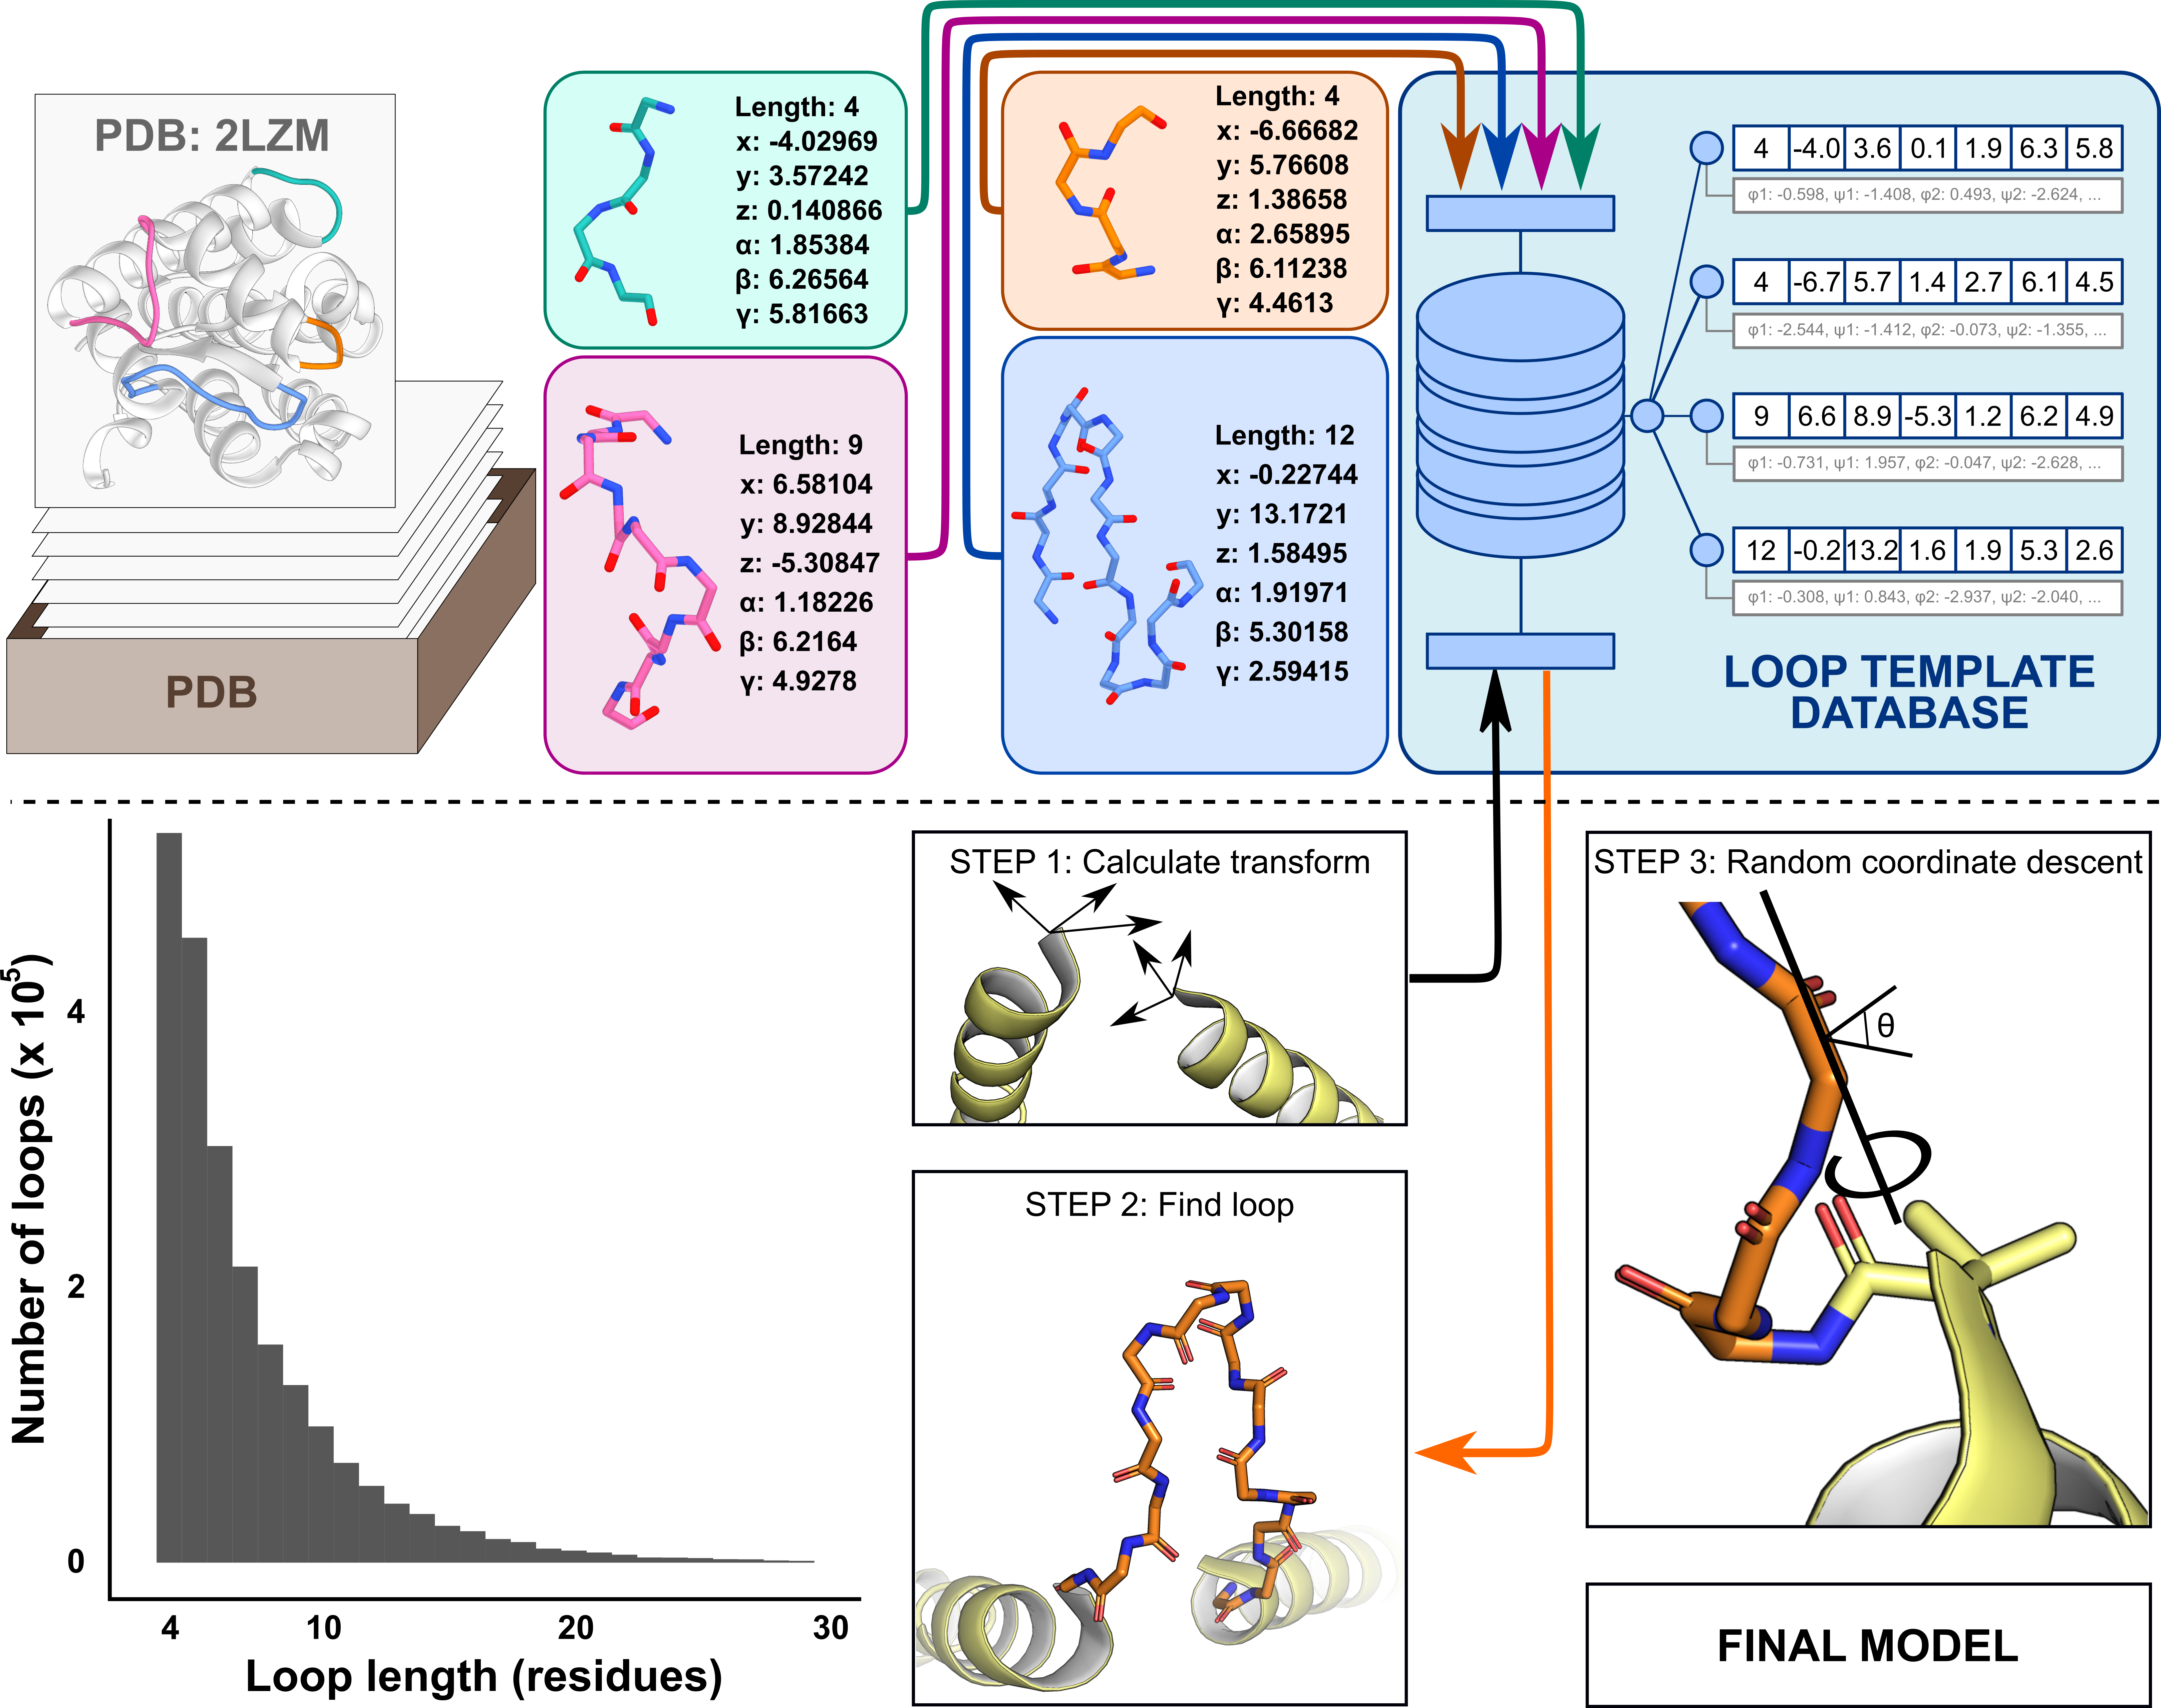
\includegraphics[width=6in]{Figures/loophash_db.pdf}
 \caption[Overview of the Hash/RCD algorithm.]{Overview of the Hash/RCD algorithm. Top: Loop parameterization using a hash key computed from the length and relative orientation of its anchor points. A hash look-up identifies and selects suitable template conformations. Bottom left: The initial template library consisted of about 3.7 million loop conformations with different sequence lengths. These loops were collected from a set of about 87,000 protein structures deposited in the PDB. Bottom right: Depiction of the conformational hashing and \gls{rcd} stages of this algorithm. An \gls{mc} framework embeds both stages and allows loop templates to be added, replaced, and removed.}
\label{fig:loophash_db}
\end{figure}

We compiled the initial template library used by the first stage from a nonredundant subset of experimentally determined structures in the PDB \citep*{Bernstein1978}. The Dunbrack lab’s protein sequence culling server (PISCES) server was used to filter out structures whose resolutions exceeded \SI{3.0}{\angstrom} and did not fully or partially consist of $\mathrm{C_{\upalpha}}$-traces \citep*{Wang2003, Wang2005}. This avoided the overrepresentation of protein structures that have been determined in multiple nearly identical conformations and resulted in about 87,000 structures. From there, we discarded the \gls{sse} definitions provided in the PDB files, instead using the \gls{sse} definition program \gls{dssp} \citep*{Kabsch1983}. Loops were defined as contiguous regions in sequence space that could not assigned any regular secondary structure. This approach both ensured reproducibility and standardized the assignment of secondary structure on the basis of backbone hydrogen bonding geometry. Finally, we removed loops containing unresolved backbone coordinates. Using this approach, we collected about 3.7 million loop conformations (Figure \ref{fig:loophash_db}).

The templates were then translated into hash keys describing the geometric aspects of the anchor residues flanking the loop (see next section for details). Lists of loops corresponding to specific geometries were stored together in a hash table. As we discuss below, Hash/RCD draws from this hash table to sample the addition and replacement of loops for given protein models by computing the parametrization of the missing loop, calculating the associated hash key, and inserting a suitable template chosen at random. The loop's sequence is then threaded over this template and inserted into the protein model. By relying on a hash table to identify templates, this approach has the advantage of $O(1)$ computation time and generally requires \gls{cpu} time on the order of microseconds. Since long loops have fewer templates in the loop library, they could be assembled from shorter fragments using a procedure discussed below.


Following conformational hashing, Hash/RCD uses random coordinate descent, previously described by Canutescu et al. \citep*{Canutescu2003} and Chys and Chacon \citep*{Chys2013}, to minimize the distance between a moving (loop end) and target (anchor) set by calculating the rotation that must occur around a given axis $({\phi},{\psi})$. We took several steps to diversify the loops generated this way. First, we found that randomly choosing which dihedral angle (either $\phi$ or $\psi$) at every step allowed Hash/RCD to avoid getting stuck in non-closable conformations. Additionally, only a random fraction of the rotation is applied. Further, we modified the original protocol to bend the terminal regions of the \gls{sse}s flanking the loop (Figure \ref{fig:loophash_db}). Finally, supplementing this protocol with scoring functions allows it to identify and reject rotations that cause the loop to clash with the rest of the protein model.

The final step of the protocol constructs the terminal loop regions. These were initialized with dihedral angles that are randomly chosen from a $({\phi},{\psi})$ distribution derived from experimentally determined protein structures. The coordinate descent algorithm was then executed to resolve steric interferences and/or energetically unfavorable configurations.

\subsection{Parametrization of loop conformations and selection of suitable conformations}

In addition to their length, loop conformations can be defined by the relative rotational and translational orientation of the anchor residues flanking them. Therefore, we defined a local orthonormal coordinate system for the anchor points of each loop as $(e_x, e_y, e_z)$ based on their backbone coordinates. Here $e_x$ is the normalized $C_{\upalpha}-C$ vector, $e_y$ is the normalized component of the $C_{\upalpha}-O$ vector orthogonal to $e_x$, and $e_z$ is computed from $e_x$ and $e_y$ such that $e_z=e_x×e_y$. Accordingly, the translation vector resides within this coordinate system and is defined as follows: 

\begin{equation}
    \vec{t}=(t_{\mathup{x}},t_{\mathup{y}},t_{\mathup{z}} )=(\alpha_{\mathup{c,x}}-\alpha_{\mathup{n,x}},\alpha_{\mathup{c,y}}-\alpha_{\mathup{n,y}},\alpha_{\mathup{c,z}}-\alpha_{\mathup{n,z}})
\end{equation}

Here $\alpha_{\mathup{c,x}}$ and $\alpha_{\mathup{n,x}}$ are the $x$-coordinates of the $C_{\mathup{\upalpha}}$-atom of the N-terminal and C-terminal anchors, respectively. The relative rotational orientation of the two anchor points was quantified using Euler angles $(\alpha,\beta,\gamma)$ following the extrinsic $x$-$y$-$z$ convention \citep*{Pio1966}. These can be readily extracted from the matrix $\mathbf{M}_{\mathup{r}}$ describing the rotation between both coordinate systems that can be computed as $\mathbf{M}_{\mathup{r}}=\mathbf{M}_{\mathup{n}}^{-1}\cdot \mathbf{M}_{\mathup{c}}$, where $\mathbf{M}_{\mathup{n}}$ and $\mathbf{M}_{\mathup{c}}$ are the transformation matrices of the local coordinate systems at the N- and C-terminal anchor points \citep*{Slabaugh1999}.

Thus, each loop was parametrized into seven parameters: the loop's sequence length ($d$), translation vector $(t_{\mathup{x}},t_{\mathup{y}},t_{\mathup{z}})$, and Euler angles $(\alpha,\beta,\gamma)$. Each parameter is discretized into bins and translated into a one-dimensional hash key $k$ using the hash function $f$:

\begin{equation}
    f:d×(t_{\mathup{x}},t_{\mathup{y}},t_{\mathup{z}} )×(\alpha,\beta,\gamma)\rightarrow k
\label{eq:loophash_hashfxn}
\end{equation}

By grouping structurally similar loops into the same bins using this function, sparse populations within the hash map are avoided. We evaluated several different bin sizes in this study and found bin sizes of \SI{1}{\angstrom} for the translation vector and 60° for the Euler angles provided the optimal balance between closure rates and accuracy. Additionally, the hash map only stores the dihedral angles $(\phi, \psi)$ of each residue in the loop conformation. As a result, each loop conformation $c$ can be described using only $2d+2$ parameters, e.g. $c=(\psi_{\mathup{N}},\phi_{1},\psi_1,…,\phi_d,\psi_d,\psi_{\mathup{C}})$. Here $d$ is the length of the loop in amino acid residues, $\psi_{\mathup{N}}$ is the $\psi$-angle of the N-terminal anchor point, $(\phi_{\mathup{i}},\psi_{\mathup{i}})$ are the dihedral angles of the $i$th residue of the loop, and $\phi_C$ is the $\phi$-angle of the C-terminal anchor point. The key-value pair $(k,c)$ of each conformation is stored in the hash map accordingly.

These steps are all carried out during the generation of the loop template prior to loop prediction. During modeling, loop look-up proceeds as follows. First, the coordinate systems for the anchor points are computed and converted into a hash function (Equation \ref{eq:loophash_hashfxn}). Second, a range of suitable conformations capable of closing this loop are returned in $O(1)$ time, and one is chosen at random. Third, the sequence of the loop being modeled is threaded onto this randomly chosen conformation, a process that happens in $O(n)$ time. Therefore, the overall time complexity of the algorithm is limited by the linear-time computation of this last step, which is in turn determined by the length of the loop being modeled.

\subsection{Integration of conformational hashing within a Monte Carlo Metropolis framework}

In a protein model containing multiple loop regions, closing a certain loop with a certain conformation might hinder the closure of other loops. Consequently, our algorithm must be able to sample different combinations of loops without needlessly increasing computational complexity. Owing to the previously demonstrated success of \gls{mc} algorithms \citep*{Leaver-fay2011, Leman2020, Karakas2012, Fischer2016a}, we embedded the conformational hashing step in an \gls{mc} framework. Effectively, the loop construction algorithm consists of two sub-algorithms, conformational hashing and \gls{rcd}, which are executed back-to-back. Each sub-algorithm places a "pseudo-residue" at the terminal end of a loop and tries to perfectly superimpose it over the corresponding anchor residue. Loop closure is calculated using the \gls{rmsd} of this pseudo-residue and the anchor residue; we use an \gls{rmsd} cutoff of \SI{0.08}{\angstrom} to account to allow for minor inaccuracies in bond lengths and angles.

In the \gls{mc} implementation of the conformational hashing algorithm (Figure \ref{fig:loophash_db}), a loop is randomly selected, perturbed, and evaluated using a scoring function. Several perturbations can be sampled. First, missing loops can be added directly from the hash map. Second, subregions of a loop can be replaced with loops added from the hash map. Third, short stretches of up to three residues can be cut back at the anchor residues and replaced with loop conformations obtained from the hash map. Fourth, when suitable loops with sequence length $d+2$ are absent from the template library, stepwise construction of loops can instead be achieved by randomly selecting loop conformations with sequence length less than $d-2$ from the template library and applying them to the selected template.

Depending on the impact of these perturbations on the score of the model, the new model is either accepted or rejected \citep*{Karakas2012}.  Knowledge-based score terms used to evaluate loop conformations include clash evaluation, consistency with Ramachandran potentials, and residue-residue interactions. We also added score terms to evaluate a model's consistency with secondary structure prediction algorithms such as PSI-blast based secondary structure Prediction \citep*{Jones1999, Ward2003}, Jufo9D \citep*{Leman2013}, and MASP \citep*{Mendenhall2014}. Finally, a score term consisting of 30\% of the scoring function pushes the algorithm toward loop closure by linearly penalizing stretches of missing residues.

\subsection{Construction of missing loop regions using random coordinate descent}

The \gls{rcd} algorithm closed loops only when they could not be closed using the conformational hashing algorithm. Its implementation is modeled on the CCD algorithm described by Canutescu et al. \citep*{Canutescu2003}, which is in turn based on the random tweak algorithm \citep*{Fine1986, Shenkin1987}; additionally, we included several modifications discussed by Chys and Chacon \citep*{Chys2013}. This portion of the algorithm can be divided into a pre-stage and a main-stage component.

During the pre-stage, missing residues are dynamically added to the anchor residues. The backbone dihedral angles of these residues are initialized with $(\phi, \psi)$ angles derived from a probability distribution of experimentally observed backbone dihedral angles. Then, using a knowledge-based potential, these $(\phi, \psi)$ angles are subsequently perturbed and evaluated. Potential inaccuracies in the secondary structure prediction are accounted for by adding and/or removing residues from the anchor \gls{sse}s. Throughout this pre-stage, sampling is guided by scoring terms evaluating the completeness of the amino acid sequence, steric interference between residues, residue-residue interactions, and the loop trajectory towards its anchor point. This module also constructed the terminal loop regions of the protein models. The main-stage portion of the algorithm iteratively uses \gls{rcd} to calculate the rotation that must occur around a given axis ($\phi$ of $\psi$) to minimize the distance between the end of the loop and the target coordinates over many iterations to close a chain break. Throughout this step, residue-residue interactions and steric interferences between residues were evaluated using scoring functions.

We found that running the conformational hashing algorithm for 500 iterations appeared to offer the best balance between performance (loop closure) and time complexity. The algorithm could be terminated early if no score improvements were identified after 50 iterations. For the \gls{rcd} algorithm, we obtained the best results when the algorithm was run for 2000 total iterations with the option of terminating early after 500 iterations without any improvements.

\subsection{Compensation for lack of templates for long loops}

The initial set of about 87,000 protein structures contained about 3.7 million loop templates. Of those, the majority of these templates (about 2.2 million) were four or more residues in length (Figure \ref{fig:loophash_db}). By contrast, only 12\% of the templates were ten or more residues in length. Moreover, longer loops cover a greater conformational space, making the conformational hashing algorithm less likely to close these loops. We developed a two-pronged approach to overcome this challenge.

First, we supplemented our algorithm with a method that combines two short loop templates into a larger loop template by superimposing the backbone coordinates of one loop's C-terminal anchor point with the backbone coordinates of the other loop's N-terminal anchor point. The resulting template has a sequence length of $d=d_1+d_2+1$, with $d_n$ being the sequence length of the $n$th template. The translation vector $\vec{t}$ and the Euler angles $(\alpha,\beta,\gamma)$ are then computed in a straightforward manner. The local coordinate system of the N-terminal anchor point of the second template is first transformed into the local coordinate system of the N-terminal anchor point of the first template. This is achieved by multiplying the first coordinate system's rotation matrix the inverse of the second coordinate system's rotation matrix, i.e., $\mathbf{M}=\mathbf{M}_2^{-1}\cdot \mathbf{M}_1$. By multiplying the translation vector $t_2$ of the second template with this matrix, the resulting translation vector can be computed by simple vector addition, i.e., $\vec{t}=t_1+(t_2\cdot \mathbf{M})$.

Nevertheless, although this approach is theoretically sound, we found that small inaccuracies, likely due the binning strategy used in the original hash map, could be propagated when templates generated this way are in turn combined into new templates. Therefore, the stored dihedral angles for both templates were recombined into a sequence consisting of $2(d_1+d_2+2)$ dihedral angles: $(\psi_{n,1},\phi_1,1,\psi_1,1,…,\phi_{1,d},\psi_{1,d},\phi_{1,\mathup{c}},\psi_{\mathup{n},2},\phi_2,1,\psi_2,1,…,\phi_{2,d},\psi_{2,d},\phi_{2,\mathup{c}})$. An artificial amino acid sequence of length $d+2$ was generated within the algorithm and fitted against the combined sequence of dihedral angles, permitting the accurate computation of this template's parameterization. 

\subsection{The benchmark set used to evaluate the algorithm}

We evaluated the performance of this algorithm using a benchmark set consisting of twenty-nine soluble and membrane proteins (Table \ref{tab:loophash_benchmark}). This included the set of soluble proteins previously used by Tyka et al. to benchmark the Rosetta Loophash algorithm \citep*{Tyka2012}, as well as the eleven membrane proteins previously used to benchmark the protein structure prediction algorithm BCL::MP-Fold \citep*{Fischer2015}. These proteins ranged in size from 57 to 1,560 residues with varying $\alpha$-helical and $\beta$-strand secondary structure content. The 195 loops in this benchmark set with four or more residues had lengths between three and 31 residues. As we described earlier, secondary structure definitions were obtained using \gls{dssp} \citep*{Kabsch1983}; loops identified this way were then removed from each of the PDB structures. Loops with stretches of missing coordinates were excluded from the benchmark set.

For the purposes of this benchmark, we used a modified loop template library in which we removed templates belonging to homologs of proteins in the benchmark set (for heterooligomers, we kept chains that were not homologous, but removed those that were). For these purposes, a cutoff of 25\% sequence identity was used when defining homology. Homologs were identified by pairwise alignment of all 87,000 proteins to each protein in the benchmark set using Clustal Omega \citep*{Sievers2011}. This reduced the size of the loop template library by 3.4\%.

\subsection{Comparison with RCD, Rosetta Loophash, and RosettaCM}

Three loop prediction protocols were compared to Hash/RCD. We used the Rosetta scoring function \emph{score4\_smooth\_cart} to score all models generated this way. The first method, \gls{rcd}, is simply the Hash/RCD algorithm without any conformational hashing. The second method, Rosetta Loophash \citep*{Tyka2012}, was modified slightly to change the focus from loop diversification to loop closure. The “relax” stage of the procedure was skipped, leaving only resampling- and minimization-based loop closure stages. Because Loophash assumes “ideal” bond length and angles, we ran the Rosetta idealize application on each structural model in the benchmark set prior to use. The same set of structures obtained in the previous section were used to create a database for Loophash (unlike our loop database, however, even regions of the protein with secondary structure were included in the Loophash database). The 195 non-terminal loops present in the benchmark set were each tested individually, in the context of the full experimentally determined structure of the remaining loops, with parameters set to skip \gls{rmsd}-based filtering. A total of 100 output structures were sampled for each loop in the benchmark set, and each output structure represents the result of 100 randomly selected database loops matching the required geometry. Although Loophash always produced models, we found that its substitution and minimization approach frequently perturbed the protein structure, even in regions outside the loop. For this reason, whenever at least one of the 100 output structures were within \SI{1}{\angstrom} $\mathrm{C_{\upalpha}}$ \gls{rmsd} from the input structure, Loophash's ability to close that loop was defined as successful. Correspondingly, if none of the output structures met this criterion, Loophash's ability to close the loop was defined as a failure. Runtimes for Loophash are reported as an average for a single output structure and include only the time spent actively sampling the loop.

The third method, RosettaCM, is a homology modeling protocol that fills loops using a hybrid approach combining fragment insertion with full-atom Cartesian minimization \citep*{Song2013}. We chose this protocol as an orthogonal approach for the purposes of benchmarking Hash/RCD for two reasons. First, it is widely used for homology modeling, a task that often involving loop prediction and closure. Second, the strategy for loop closure, which involves the insertion of three- and nine-residue fragments followed by Cartesian minimization, is superficially similar to the strategy used by Hash/RCD. The fragment templates used by RosettaCM were obtained from the Robetta web server with homologs excluded \citep*{Kim2004}. During the coarse-grained stages of the protocol, the \emph{atom\_pair\_constraint} score term was set to 5.0 and the \emph{frag\_weight\_aligned} option was set to 0.0 to avoid modifying non-loop regions. The full-atom Cartesian minimization step was then carried out with coordinate constraints from the starting model. Models were then scored using the scoring function \emph{ref2015\_cart}. Because RosettaCM explicitly models all sidechains and has an execution time ranging from minutes to hours, we do not report runtimes for this protocol and use it only to compare the \gls{rmsd} values of the resulting models.

\section{Results}

This section describes the distribution of templates collected from structures in the PDB and rationalizes the need for template recombination. Following this, the performance of the conformational hashing algorithm is reported using loop closure rate and compute time. Additionally, we discuss the algorithm's performance as a function of different optimization parameters. This section concludes with a comparison of models generated by Hash/RCD, \gls{rcd} alone, Rosetta Loophash, and RosettaCM.

\subsection{Effect of parameter bin size and loop length on loop closure by conformational hashing}

Before computing the hash key for a loop template, the loop’s parametrization needs to be discretized, which is achieved through binning (see Section \ref{sec:loophash_methods}). The hash map's granularity is heavily influenced by the bin width, which in turn significantly influences the closure rate and physical reasonableness of the loop regions it generates. For example, whereas larger bin widths are more densely populated, the resulting loop regions can be physically unreasonable. Smaller bin widths, by contrast, result in a sparser population of the hash map and come at the cost of a lower loop closure rate. Therefore, we quantified the influence of the bin width on the loop closure rate by repeating loop construction for the benchmark set with different bin widths. Specifically, the rotation bin width was increased in 30° steps from 30° to 120° (the translation bin width was kept at \SI{1}{\angstrom} because larger translation bin widths would require post-processing of the fitted loop to avoid overextension of the peptide bonds). This evaluation did not use a post-processing step, such as minimization, to reduce computational complexity.

The results are shown in Figure \ref{fig:loophash_closurerate} and demonstrate how loop closure rate decreased approximately linearly with loop length. For example, among loops no more than five residues long, a bin width of 60° led to a loop closure rate of 94\%. Among loops between six and ten residues long, however, it dropped to 61\%, and for loops greater than ten residues long, it fell further to 33\%, for an average total loop closure rate of 70\%. We observed a similar, almost linear relation between loop length and loop closure rates when using the other three evaluated angle bin widths. More generally, we found that loop closure strongly depended on angle bin width. For the evaluated angle bin widths of 30°, 60°, 90°, and 120°, the total loop closure rate of the conformational hashing algorithm arrived at 58\%, 70\%, 78\% and 89\% (Figure \ref{fig:loophash_closurerate}). Although these results suggest that larger angle bin widths are preferable, upon closer examination we found that many of the resulting models revealed had unnatural angles within the peptide bonds connecting the anchor \gls{sse}s and the loop. Rather than increase the computational complexity of the algorithm by using minimization or other post-processing steps, we opted for an angle bin width of 60°.

\begin{wrapfigure}{R}{0.55\textwidth}
\centering
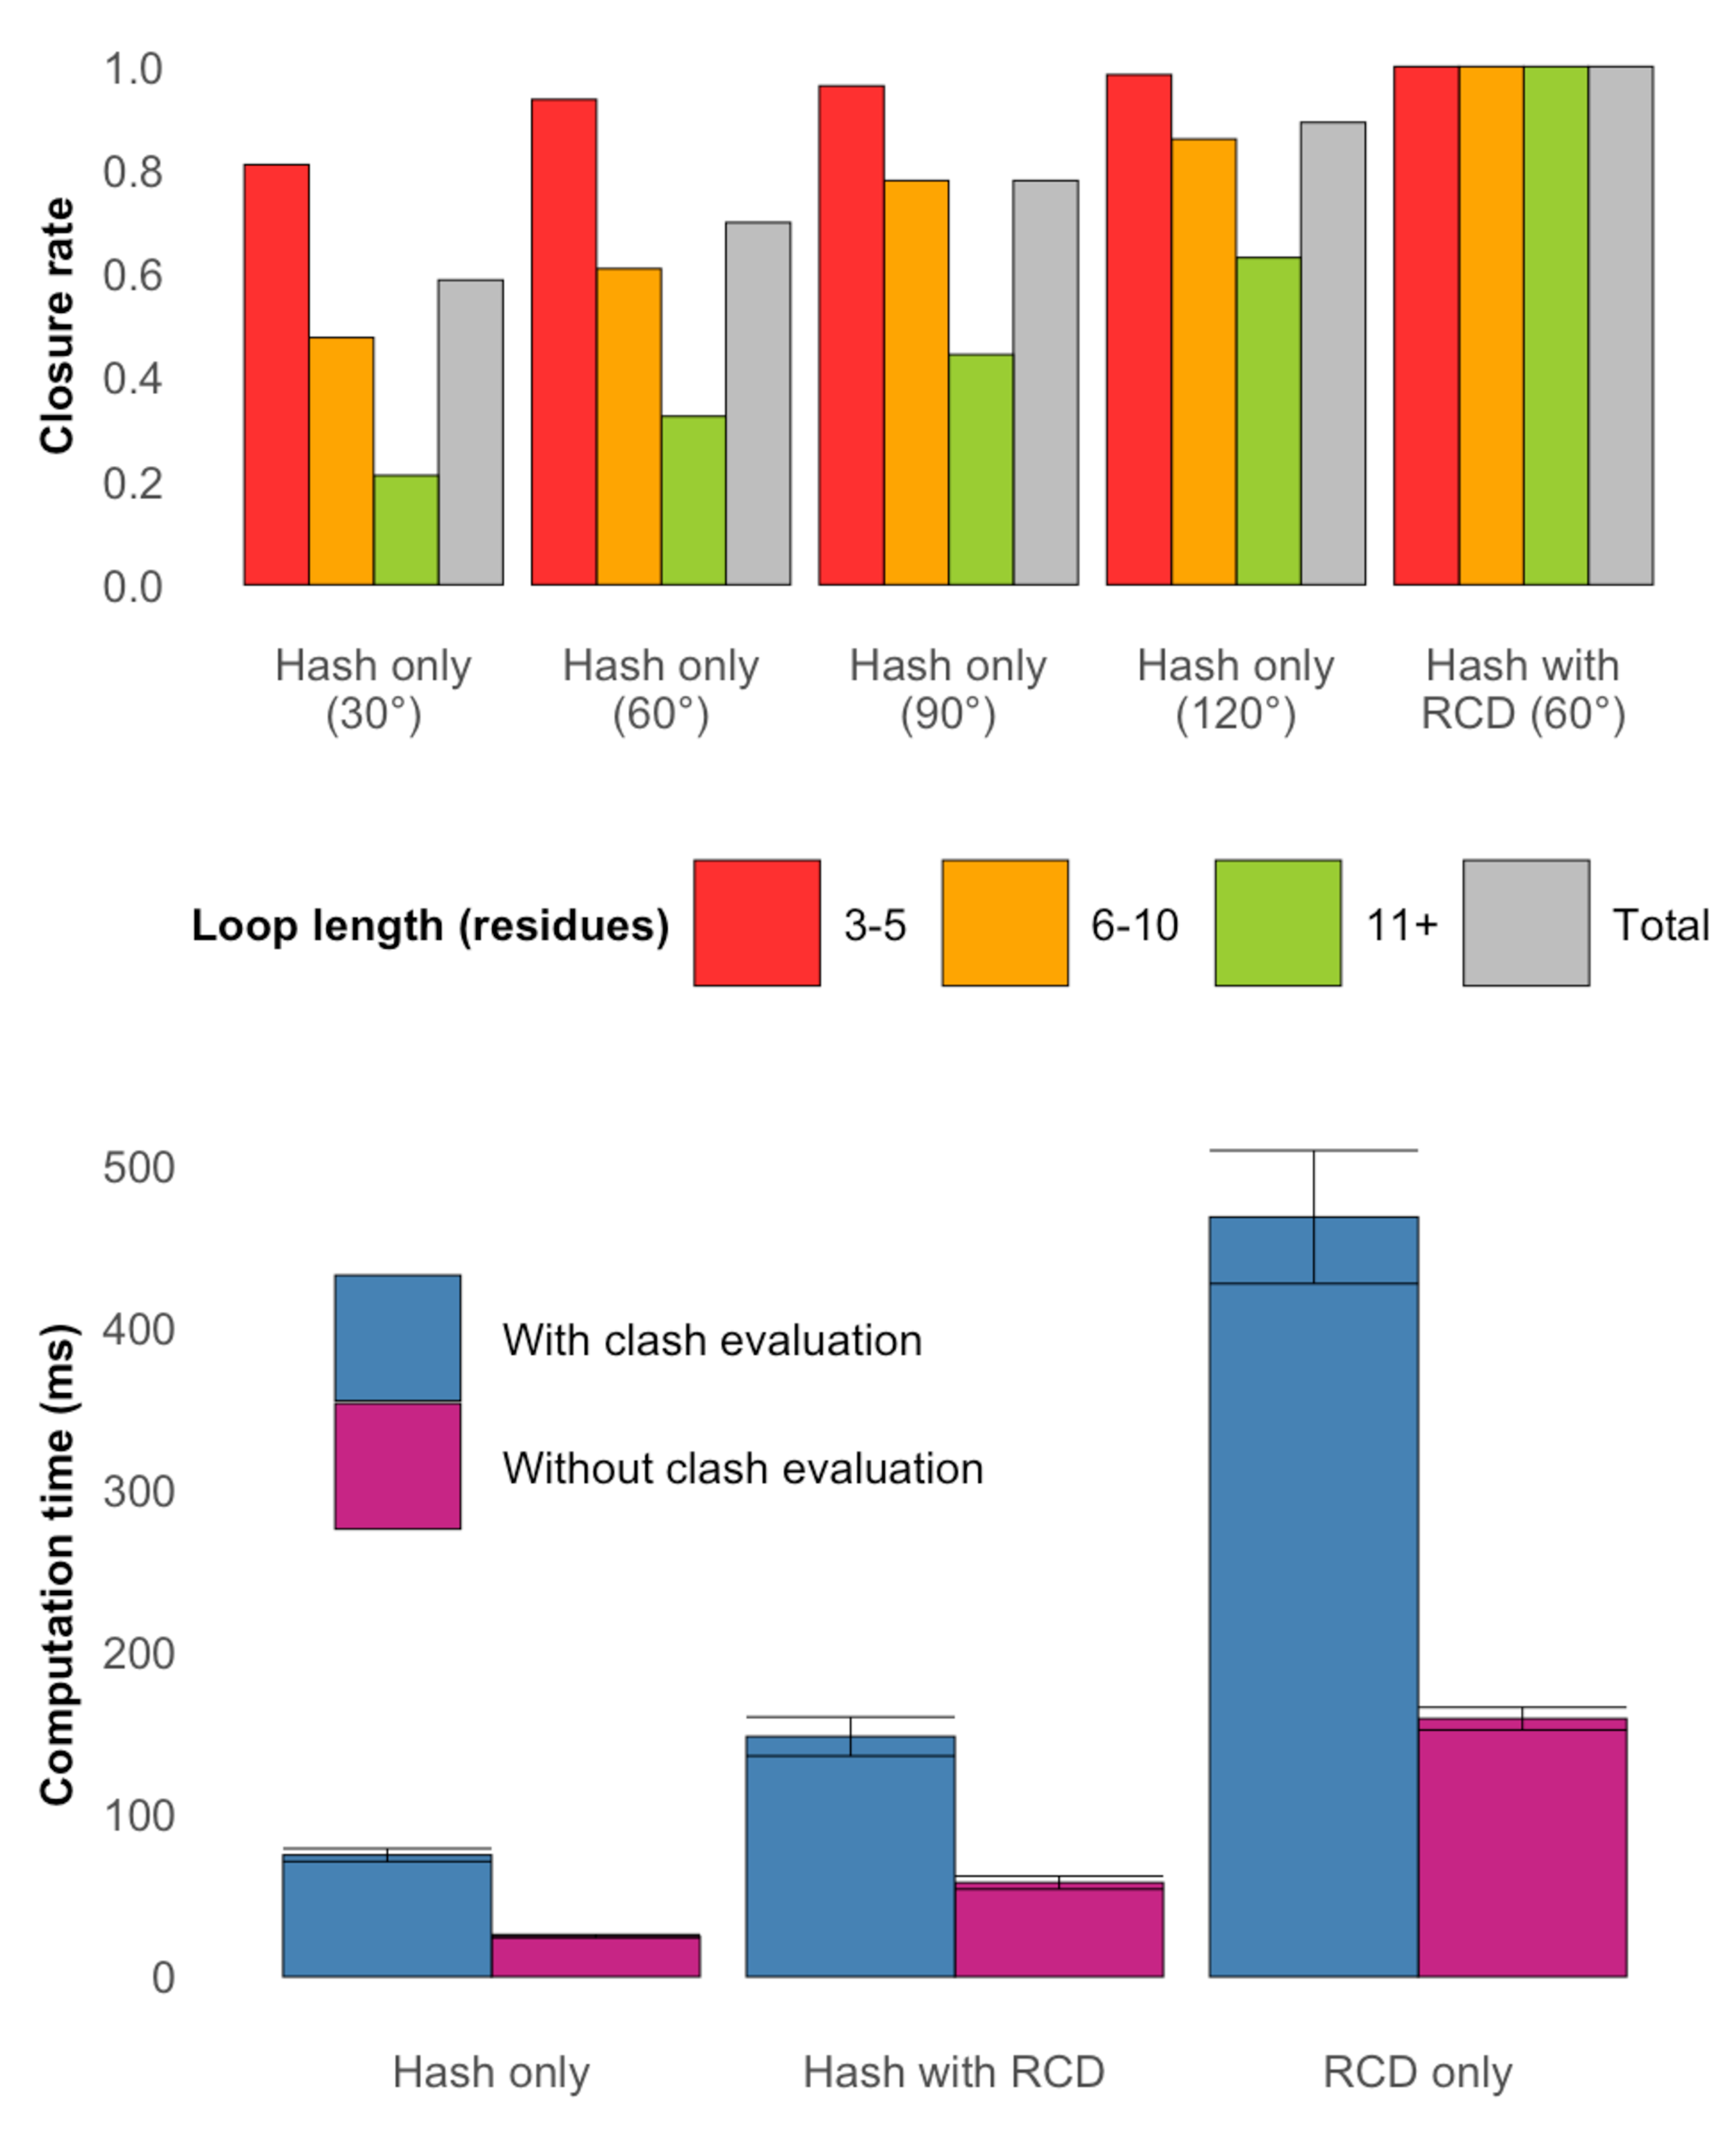
\includegraphics[width=3.25in]{Figures/loophash_closurerate.pdf}
 \caption[Evaluating conformational hashing and \gls{rcd} algorithms for loop construction.]{Evaluating conformational hashing and \gls{rcd} algorithms for loop construction. Top: The rotation angle bin width of the hash map influenced the loop closure rate of longer loops when using conformational hashing alone. When modeling short loops, we found high loop closure rates regardless of bin width. When conformational hashing was combined with \gls{rcd}, the loop closure rate increased to 100\% in our benchmark set. Bottom: The calculation of steric interference constituted the overwhelming majority of this algorithm's \gls{cpu} time requirement. Combining conformational hashing with \gls{rcd} was found to improve \gls{cpu} time efficiency.}
\label{fig:loophash_closurerate}
\end{wrapfigure}
 
\subsection{Conformational hashing achieves a high loop closure rate for short loops but RCD is required for long loops}

We evaluated the percentage of missing loop regions among our benchmark set (Table \ref{tab:loophash_benchmark}) that could be successfully constructed by first removing all non-terminal loop regions from each protein structure. We then constructed the missing loop regions using our algorithm and computed the loop closure rate per benchmark protein. This was performed with the original template library either prior to or following extension by template recombination and fragment-based loop construction (see section \ref{sec:loophash_methods}). In both cases, the loop libraries were binned at 60°.

When additional templates through fragment combination are excluded, the algorithm achieved a loop closure rate of 54\% over all twenty-nine benchmark proteins. As demonstrated above, a loop's length strongly influenced whether it could be successfully closed. For example, loops up to five residues long were successfully closed 87\% of the time, whereas loops ten residues long or greater were closed only 21\% of the time. By contrast, when the template library was extended to include loops generated using fragment-based construction, the overall loop closure rate could be improved by nearly 30\% to an overall closure rate of 70\% (Figure \ref{fig:loophash_closurerate}). Further increases in either the size of this library through additional fragment recombination did not appear to improve loop closure rate (data not shown). Nevertheless, as we mentioned above, following this step with \gls{rcd} achieved a closure rate of 100\%.
We found that Rosetta Loophash achieves a 99\% loop closure rate on the loops with a length of ten residues or less. However, this plummeted to 39\% when loop length exceeded ten residues. We note that this high loop closure rate is achieved in part by using a \SI{2}{\angstrom} bin width, which is wider than the \SI{1}{\angstrom} width used by Hash/RCD. A consequence of this approach is its reliance on optimization and refinement following the fitting, which increases the computational effort required (discussed below).

\subsection{CPU time requirement is dominated by the evaluation of steric interference}

Although the time complexity of the template look-up is O(1), the task of threading the target sequence against the template is O(n), which leads to linear time complexity for the overall loop construction algorithm. We therefore studied the effect this had on the CPU time required to execute the algorithm (specifically, the time between entering the \gls{mc} algorithm and leaving the \gls{mc} algorithm divided by the number of successfully constructed loop regions). To evaluate the contribution of the scoring term evaluating steric interference between residues relative to the overall CPU time requirement, the computation time needed by this term was evaluated separately. This was repeated for both \gls{rcd} alone and Hash/RCD.

When steric interference was not included during sampling, conformational hashing required on average 27±\SI{4}{ms} \gls{cpu} time per loop, whereas \gls{rcd} required 159±\SI{11}{ms}. By contrast, Hash/RCD required only 68±\SI{7}{ms} (Figure \ref{fig:loophash_closurerate}). When steric interference is calculated during sampling, the required CPU time increased to 59±5 ms for conformational hashing, 468±41 ms for RCD, and 161±13 ms for Hash/RCD. The evaluation of steric interferences dominated the computational burden by accounting for 54\%, 66\%, and 58\% of the total CPU time requirement among conformational hashing, \gls{rcd}, and Hash/RCD, respectively. Overall, these results demonstrate that using templates prior to coordinate descent can lead to a threefold decrease in the computation time of loop closure.

In contrast, the Rosetta Loophash protocol has a CPU runtime of \SI{160}{s} to sample each loop. This runtime is highly correlated with total protein size ($R^2=0.8$). We found that it is overwhelmingly devoted to minimization, as only 5\% of the algorithm's runtime involved conformational sampling.

\newpage

\subsection{Hash/RCD samples experimentally observed conformations}

Hash/RCD was developed to efficiently sample both major and minor populations that a loop might adopt. We assume that the experimentally determined structures deposited in the PDB correctly and accurately represent one of the proteins’ major populations (minor populations, by contrast, can only rarely be verified experimentally and are not considered for this benchmark). To test whether Hash/RCD correctly samples those conformations, we generated 100 models with constructed loop regions for each protein in the benchmark set. These conformations were subsequently compared to the experimentally determined structures using the \gls{rmsd} of the $\mathrm{C_{\upalpha}}$-atoms. For the membrane protein structure 3P5N, two non-terminal loops were not resolved in the X-ray-derived model and consequently excluded from this comparison. Moreover, in the case of homo-oligomeric proteins in the benchmark set, we excluded each instance of a given loop beyond the first to avoid their overrepresentation in the benchmark set. This led to 195 non-terminal loops comprised of three or more residues.

To focus on how effectively Hash/RCD could sample the major loop population, we determined the loop with the lowest $\mathrm{C_{\upalpha}}$ \gls{rmsd} among each of the 100 conformers sampled for each of the 195 loops in the benchmark set (Figure \ref{fig:loophash_rmsd}, top left). As expected, the lowest \gls{rmsd} among the conformers we sampled depended on the length of the loop, which in turn dictated the size of the sampling space. However, in the majority of loops, at least one conformer was within \SI{2}{\angstrom} of the experimentally observed structure, and all of the longer loops sampled at least one conformer within \SI{5}{\angstrom} $\mathrm{C_{\upalpha}}$ \gls{rmsd}. We found that these results were comparable to those obtained using \gls{rcd} alone, as well as the orthogonal hybrid method RosettaCM. In sharp contrast, Rosetta Loophash was far less capable of sampling native-like loop conformers with lengths exceeding ten residues. These results suggest that the lack of long templates prevents these loops from being closed using physiologically meaningful structures, and that sampling becomes the predominant obstacle for modeling long loops using conformational hashing.
 
\begin{figure}[h!]
\centering
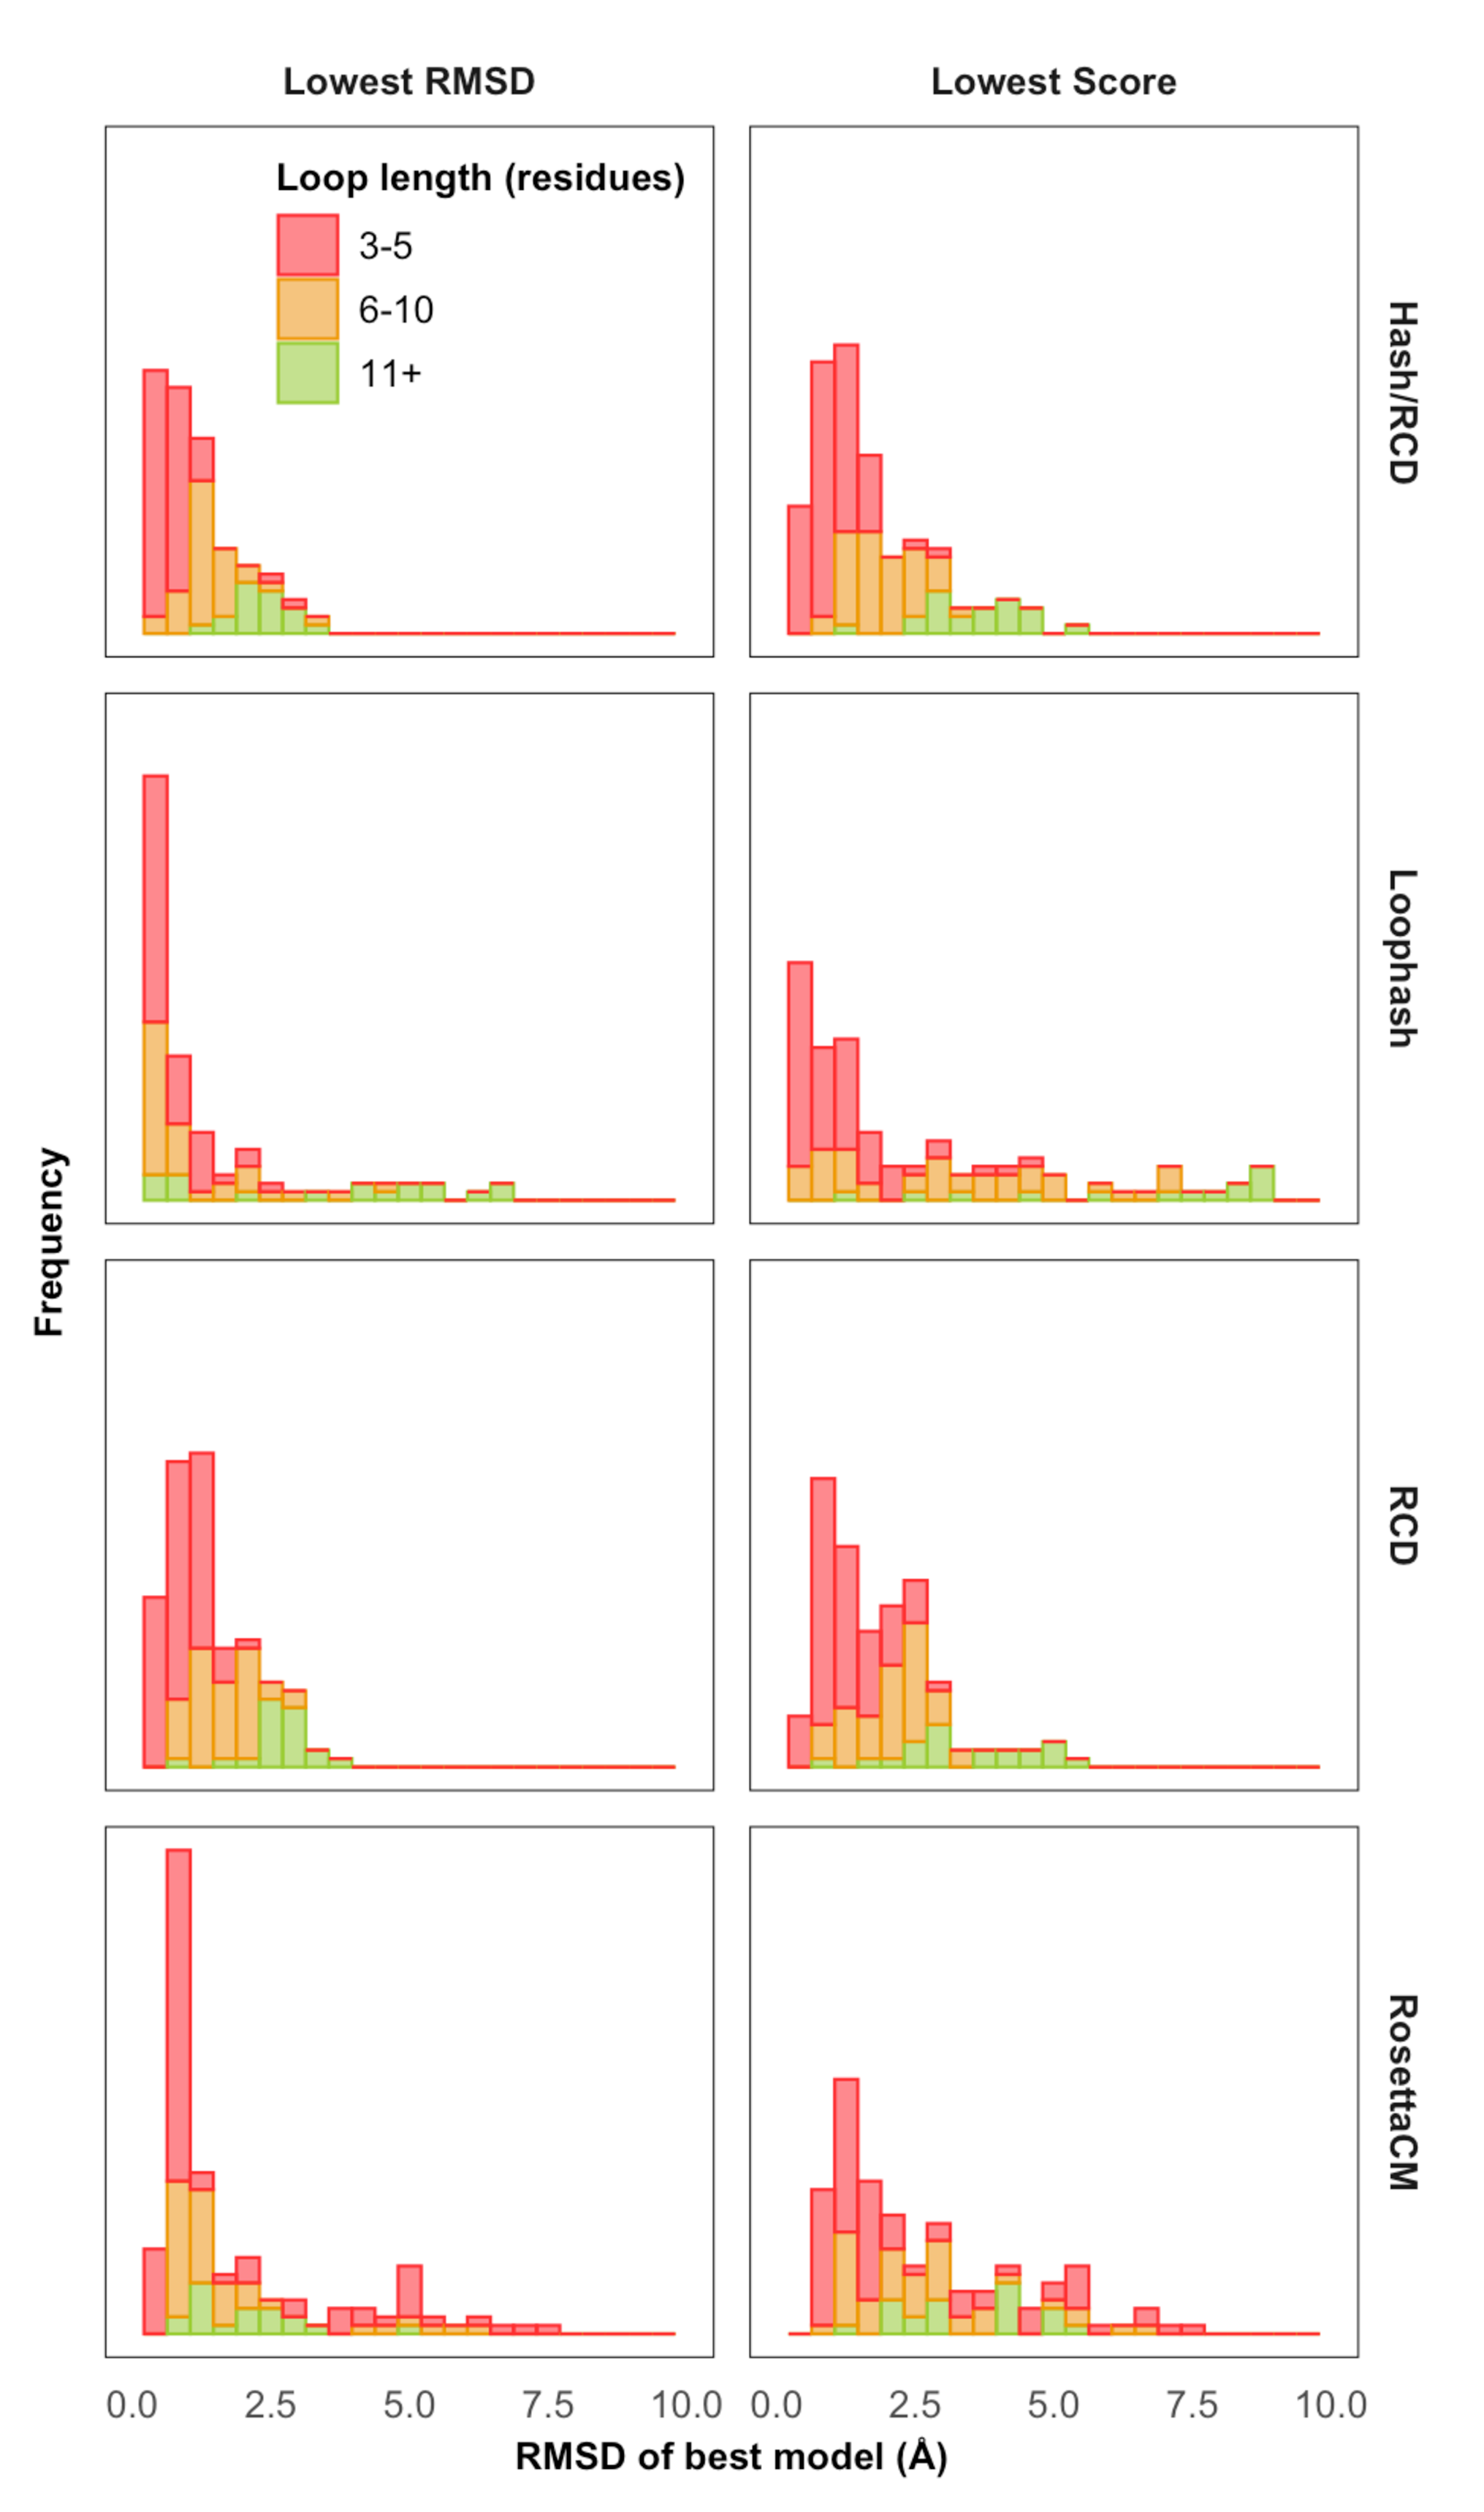
\includegraphics[width=3.25in]{Figures/loophash_rmsd.pdf}
 \caption[Loops generated using Hash/RCD are comparable in quality to those using RCD alone.]{Loops generated using Hash/RCD are comparable in quality to those using RCD alone. Left: Histograms of the lowest \gls{rmsd} values among loop conformers sampled by a variety of methods. Although Rosetta Loophash slightly outperformed Hash/RCD, \gls{rcd} alone, and RosettaCM when modeling short loops, it was unable to model native-like conformations for long loops. Right: Histograms of the \gls{rmsd} values of the lowest-scoring loop conformers.}
\label{fig:loophash_rmsd}
\end{figure}

When native loop conformations are unavailable and \gls{rmsd} values cannot be calculated, scoring functions must be used to infer which loop conformers are structurally relevant. We therefore focused on the lowest-scoring loops obtained using each method. Distributions are shown in Figure \ref{fig:loophash_rmsd} (right panels), and pairwise comparisons between Hash/RCD and other methods are shown in Figure \ref{fig:loophash_comparison}. The results reinforce the findings discussed above. Notably, the lowest-scoring loop conformer in most cases had \gls{rmsd} values only slightly higher than the lowest-\gls{rmsd} loop. We interpret this to suggest that the sampling space of the Hash/RCD method is focused on native-like conformers and ignores portions of the conformational space that are unlikely to be physiologically relevant. Moreover, these \gls{rmsd} values are comparable to those obtained from the lowest-scoring loops obtained using \gls{rcd} alone and contrast with the lowest-scoring conformers of long loops obtained by Rosetta Loophash. Finally, they improve upon loop modeling using RosettaCM, which interestingly was less effective at predicting short loops than we expected but reproduced the model quality of long loops that was observed using either Hash/RCD or \gls{rcd} alone.

Our results highlight the shortcomings of an exclusively template-based strategy when attempting to model long loops. When taken alongside the improvements in computation time, the results suggest that Hash/RCD arrives at conformations similar in quality to \gls{rcd} alone, but skips over a large number of intermediate conformations that would otherwise be expensive to sample. By further improving conformations obtained using conformational hashing, Hash/RCD achieves results comparable to \gls{rcd} alone on computational timescales comparable to those of template-based methods.

\newpage

\section{Discussion}

\begin{wrapfigure}{r}{0.4\textwidth}
\centering
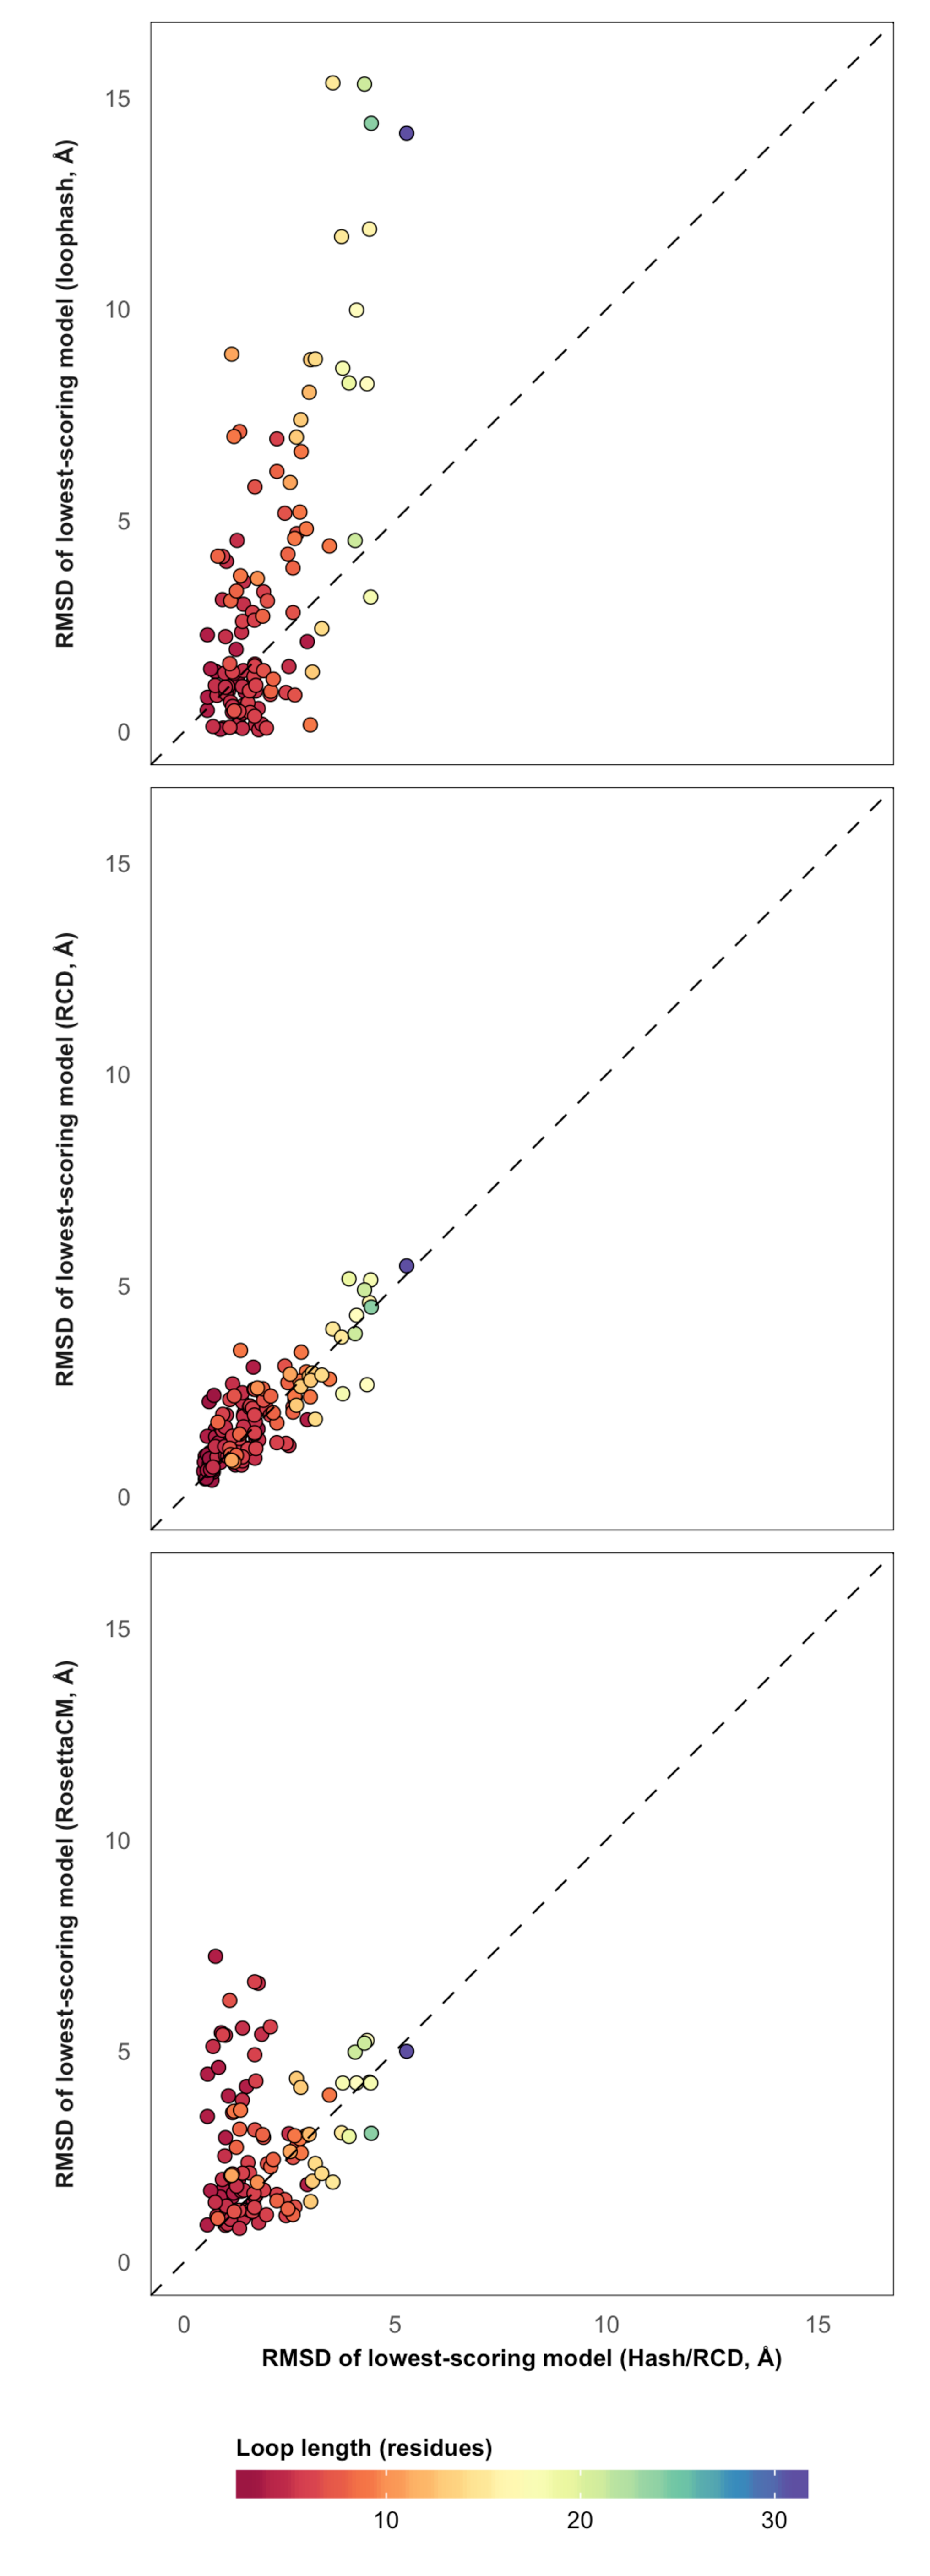
\includegraphics[width=2.35in]{Figures/loophash_comparison.pdf}
 \caption[Pairwise comparison of RMSD values among the best-scoring loop conformations obtained using Hash/RCD, Rosetta Loophash, RCD alone, or RosettaCM.]{Pairwise comparison of RMSD values among the best-scoring loop conformations obtained using Hash/RCD, Rosetta Loophash, RCD alone, or RosettaCM.}
\label{fig:loophash_comparison}
\end{wrapfigure}

\subsection{Complementing conformational hashing with template-independent modeling}

Loop modeling algorithms that employ conformational hashing methods must address the fact that most loops found in structures deposited in the PDB have sequence lengths of less than ten residues. This is evidenced by our initial loop library, which was derived from about 87,000 protein structures and disproportionately consists of short loops (Figure \ref{fig:loophash_db}). Additionally, longer loops can cover a larger conformational space, further impeding construction of long loops using conformational hashing. When we designed Hash/RCD, we found that this led to discrepancies between the loop closure rates for different loop lengths. For example, whereas loops between three to five residues long were closed 96\% of the time, the loop closure rate dropped to 61\% and 33\% among loops with lengths of either six to ten residues or eleven or more residues, respectively. (Figure 2). We mitigated this problem by using template recombination and fragment-based loop construction (see section \ref{sec:loophash_methods}), which improved the loop closure rate from 54\% to 70\%. Nonetheless, these results reinforced the need for template-independent conformational sampling. In this study, we integrated and applied an implementation of random coordinate descent to portions of loops that could not be constructed by conformational hashing, which compensated for the latter’s inability to close long loops. As a result, loop closure improved to 100\%. Consequently, whereas a stand-alone conformational hashing approach might suffice when the goal is to construct very short loop regions, loops found in most proteins will require a hybrid template-based/template-independent loop construction algorithm.

\subsection{Hash/RCD efficiently samples structurally diverse loop conformations}

Prediction of structural heterogeneity in proteins can be achieved by sampling diverse conformations (Figure \ref{fig:loophash_gallery}), which could capture major and minor populations of the protein in equilibrium. Random coordinate descent, although computationally demanding, achieves a high loop closure rate that cannot be replaced by more \gls{cpu}-efficient template-based methods. Relying on \gls{rcd} only in cases where conformational hashing was unsuccessful led to a significant reduction in \gls{cpu} time; this was demonstrated by a drop from 468ms using \gls{rcd} alone to \SI{161}{ms} using Hash/RCD (Figure \ref{fig:loophash_closurerate}). Thus, integrating conformational hashing with \gls{rcd} combines the efficiency of conformational hashing with the high loop closure rate of \gls{rcd}. The reduction in CPU time allows a wider range of possible loop conformations to be considered (Figure \ref{fig:loophash_comparison}). However, it needs to be noted that for longer loops in the benchmark set, the conformation of the experimentally determined structure was not sampled in any of the models to within \SI{2}{\angstrom} (Figure \ref{fig:loophash_rmsd}). Since this problem was exclusively faced by loops longer than ten residues in length, it can be solved by incorporating experimental data from technique such as electron paramagnetic resonance spectroscopy or fluorescence resonance energy transfer, to reduce the size of the conformational space. Alternatively, models obtained using Hash/RCD can be further refined in molecular dynamics simulations, which may save considerable sampling time and assist in identifying more physiologically relevant loop conformers.

\begin{figure}[h!]
\centering
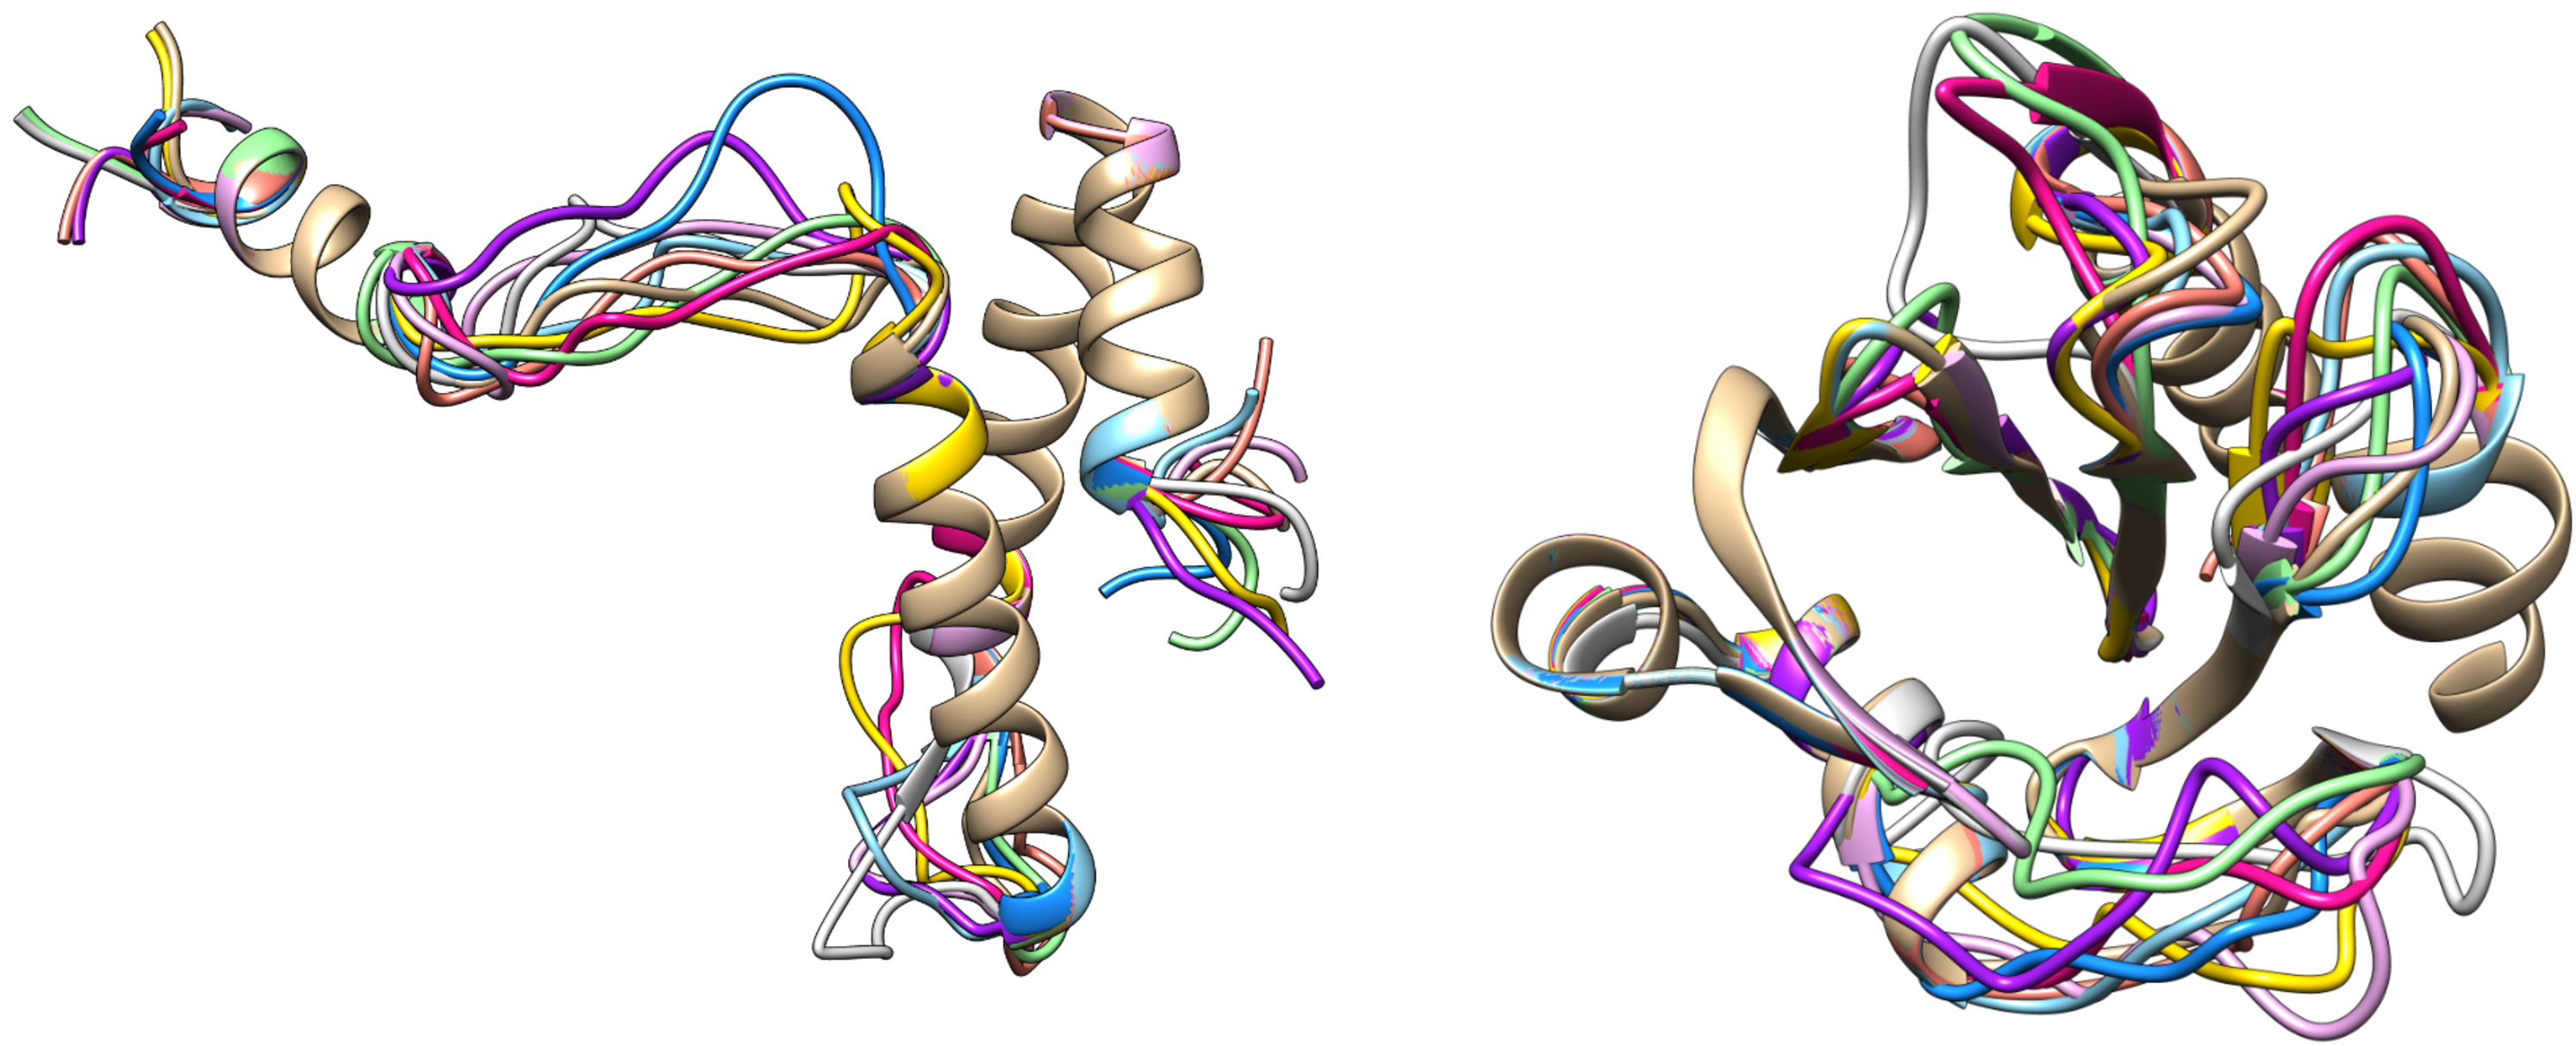
\includegraphics[width=5.5in]{Figures/loophash_gallery.pdf}
 \caption[Representative loop predictions obtained using Hash/RCD.]{Representative loop predictions obtained using Hash/RCD.}
\label{fig:loophash_gallery}
\end{figure}

\section{Conclusion}

The hybrid loop modeling method Hash/RCD provides an efficient way to sample structurally diverse loop conformations and is significantly faster than using the template-independent approach \gls{rcd} alone. We found that the constructed loop regions largely exhibit naturally occurring dihedral angles due to their construction from experimentally observed conformations. While this algorithm’s millisecond-timescale computation time was only quantified when implemented in the \gls{bcl}, we believe similar performance can be theoretically achieved in any protein structural modeling program.

Two applications of this approach are proposed. First, it could be used for the prediction of conformational ensembles in loop regions. For example, one could conceivably fit these loops against experimental data to determine a weighted distribution of conformers that represents the protein in question under equilibrium conditions. Second, the simultaneous prediction of adjacent loops could reveal a protein’s topological details, for example by capturing to what extent two loops may be intertwined. This may be relevant to multipass integral membrane proteins, as their solvent-exposed loop regions are least likely to be resolved.

\section{Acknowledgments}

We want to thank Dr. Marion F. Sauer for thorough proofreading of this manuscript. Work in the Meiler laboratory is supported through NIH (R01 GM080403 and R01 GM073151). The authors acknowledge funding by the Deutsche Forschungsgemeinschaft (DFG, German Research Foundation) through SFB1423, project number 421152132, subproject A07 and Z04. Parts of the data analysis were performed using R in conjunction with the ggplot2 package \citep*{Wickham2009}. Figures depicting protein models were created using Chimera \citep*{Pettersen2004} and composite figures were created using Inkscape. To determine sequence identities between the template set and the benchmark set, the sequences were aligned using Clustal Omega \citep*{Sievers2011}.


\clearpage % clear the prior chapter's page

\chapter{Supplement to "Rapid simulation of unprocessed DEER decay data for protein fold prediction"} \label{app:rosettadeer_supp}
%\vspace{-7mm}
%\bigskip

This Appendix contains supplementary information for Chapter \ref{ch:rosettadeer}.

\begin{table}[h!]
\scriptsize
\renewcommand{\tabcolsep}{0.09cm}
\centering
\caption[List of spin-labeled proteins in the Protein Databank.]{List of spin-labeled proteins in the Protein Databank.}

\newcolumntype{Y}{>{\raggedright\arraybackslash}X}

\begin{center}
\begin{tabular}{l l l l r}
\toprule \\
\textbf{Protein} & \textbf{PDB} & \textbf{Angle} & \textbf{Distance} & \textbf{Ref.} \\
T4 Lysozyme & 1ZYTa & 5.23  & 0.83 & \citep*{Fleissner2009} \\
T4 Lysozyme & 2CUUa & 7.24  & 0.84 & \citep*{Fleissner2009} \\
T4 Lysozyme & 2CUUa & 3.39  & 0.78 & \citep*{Fleissner2009} \\
T4 Lysozyme & 2IGCa & 11.49 & 0.81 & \citep*{Guo2008} \\      
T4 Lysozyme & 2NTHa & 3.06  & 0.8  & \citep*{Guo2008} \\      
T4 Lysozyme & 2OU8a & 7.13  & 0.82 & \citep*{Guo2008} \\      
T4 Lysozyme & 2OU8a & 9.08 & 0.86 & \citep*{Guo2008} \\      
T4 Lysozyme & 2OU9a & 15.13 & 0.84 & \citep*{Guo2008} \\      
T4 Lysozyme & 2Q9Da & 10.99 & 0.8  & \citep*{Guo2008} \\      
T4 Lysozyme & 2Q9Ea & 14.55 & 0.86 & \citep*{Guo2008} \\      
T4 Lysozyme & 2Q9Eb & 14.55 & 0.86 & \citep*{Guo2008} \\      
T4 Lysozyme & 2Q9Ec & 8.08  & 0.84 & \citep*{Guo2008} \\      
GB1         & 3V3Xb & 4.78  & 0.83 & \citep*{Cunningham2012} \\ 
GB1         & 3V3Xb & 8.53  & 0.82 & \citep*{Cunningham2012} \\ 
GB1         & 3V3Xb & 1.13  & 1.02 & \citep*{Cunningham2012} \\ 
GB1         & 3V3Xc & 2     & 0.8  & \citep*{Cunningham2012} \\ 
GB1         & 3V3Xd & 5.65  & 0.78 & \citep*{Cunningham2012} \\ 
GB1         & 3V3Xd & 1.39  & 0.8  & \citep*{Cunningham2012} \\ 
GB1         & 3V3Xd & 2.71  & 0.81 & \citep*{Cunningham2012} \\ 
%P450cam     & 4EK1a & 5.64  & 0.78 & \citep*{Still2012}      \\ 
%P450cam     & 4EK1b & 8.46  & 0.8  & \citep*{Still2012}      \\ 
GB1         & 5BMGa & 10.97 & 1.08 & \citep*{Cunningham2016} \\ 
GB1         & 5BMGb & 4.57  & 0.79 & \citep*{Cunningham2016} \\ 
GB1         & 5BMGc & 13.52 & 1.13 & \citep*{Cunningham2016} \\ 
GB1         & 5BMGd & 5.89  & 0.8  & \citep*{Cunningham2016} \\ 
GB1         & 5BMGe & 1.45  & 0.99 & \citep*{Cunningham2016} \\ 
GB1         & 5BMGf & 7.7   & 0.84 & \citep*{Cunningham2016} \\ 
GB1         & 5BMGg & 8.47  & 0.87 & \citep*{Cunningham2016} \\ 
GB1         & 5BMHa & 8.29  & 0.77 & \citep*{Cunningham2016} \\ 
GB1         & 5BMHa & 9.38  & 0.77 & \citep*{Cunningham2016} \\ 
GB1         & 5BMIa & 7.42  & 0.83 & \citep*{Cunningham2016} \\ 
Azurin      & 5I26a & 4.8   & 0.81 & \citep*{Consentius2016} \\ 
Azurin      & 5I26b & 0.55  & 0.99 & \citep*{Consentius2016} \\ 
Azurin      & 5I26c & 0.92  & 1.01 & \citep*{Consentius2016} \\ 
Azurin      & 5I26d & 0.89  & 1    & \citep*{Consentius2016} \\ 
Azurin      & 5I28a & 0.5   & 1    & \citep*{Consentius2016} \\ 
Azurin      & 5I28b & 0.71  & 1    & \citep*{Consentius2016} \\ 
Azurin      & 5I28c & 0.32  & 1.01 & \citep*{Consentius2016} \\ 
Azurin      & 5I28d & 0.25  & 1.01 & \citep*{Consentius2016} \\ 
Azurin      & 5I28e & 4.49  & 0.96 & \citep*{Consentius2016} \\ 
Azurin      & 5I28f & 1.81  & 1.01 & \citep*{Consentius2016} \\ 
Azurin      & 5I28f & 2.15  & 0.98 & \citep*{Consentius2016} \\ 
Azurin      & 5I28h & 2.1   & 0.89 & \citep*{Consentius2016} \\ 
Azurin      & 5I28i & 5.44  & 0.8  & \citep*{Consentius2016} \\ 
Azurin      & 5I28j & 6.8   & 0.85 & \citep*{Consentius2016} \\ 
T4 Lysozyme & 5JDTa & 2.52  & 0.78 & \citep*{Consentius2016} \\ 
T4 Lysozyme & 5JDTa & 0.85  & 0.76 & \citep*{Consentius2016} \\ 
\bottomrule \\
\end{tabular} 
\end{center}
\label{tab:rosettadeer_main_slproteins}
\end{table}

\begin{figure}[h]
\centering
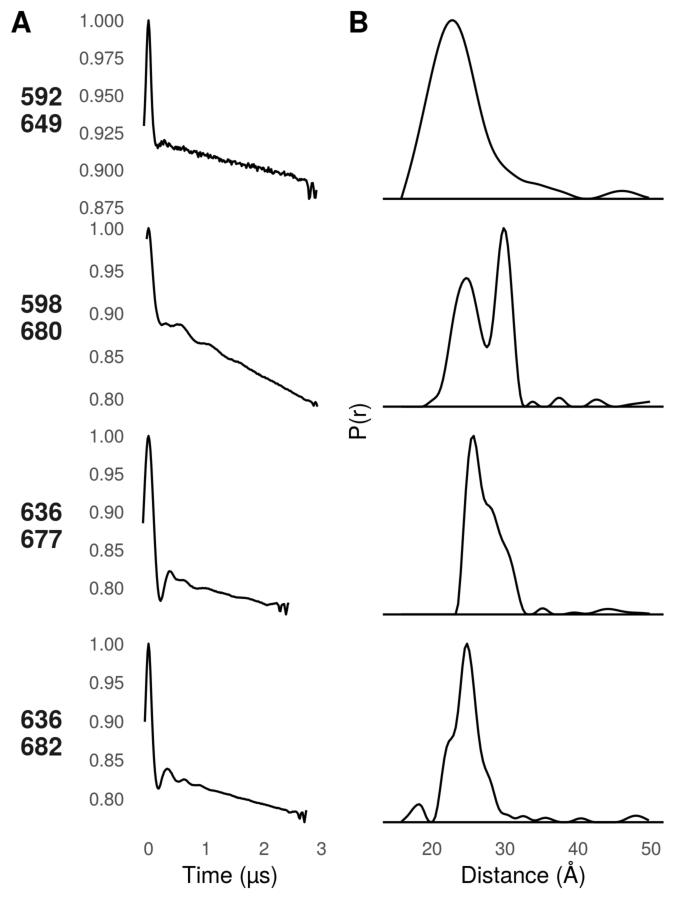
\includegraphics[width=4in]{Figures/rosettadeer_supp_exou.pdf}
 \caption[Data gathered in the ExoU C-terminus for this study.]{Data gathered in the ExoU C-terminus for this study.}
\label{fig:rosettadeer_supp_exou}
\end{figure}

\begin{figure}[h]
\centering
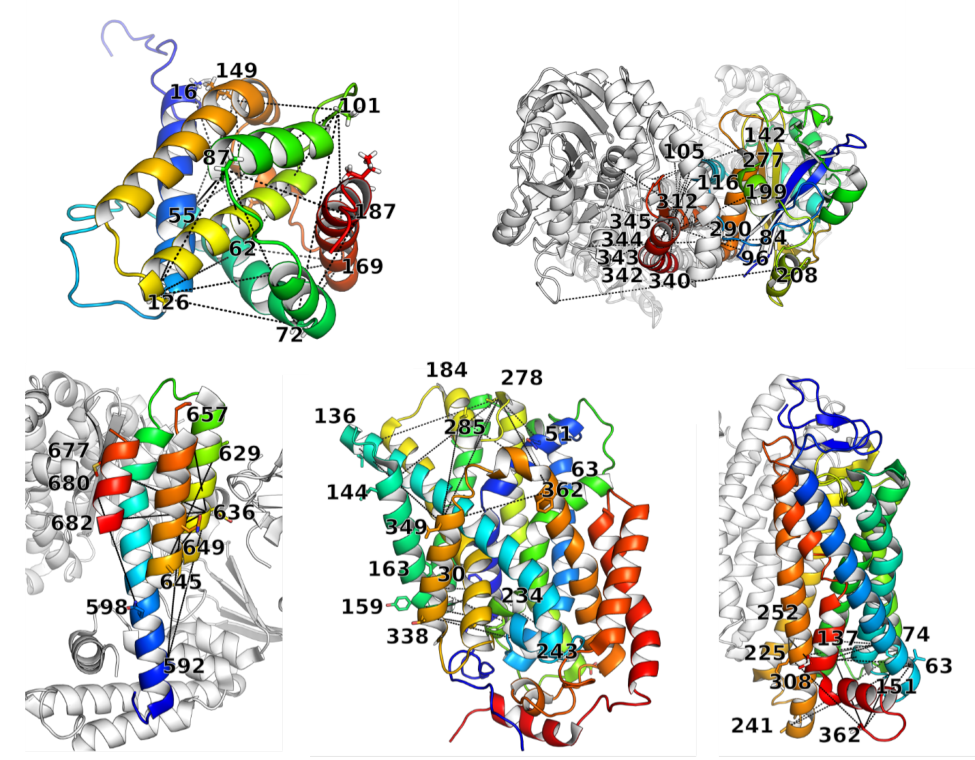
\includegraphics[width=5.5in]{Figures/rosettadeer_supp_restraints.pdf}
 \caption[Placement of experimental DEER restraints on protein structures used in this study.]{Placement of experimental DEER restraints on protein structures used in this study. Clockwise from top left: Bax (PDB: 1F16 model 8), CDB3 (PDB: 1HYN chains R/S), Rhodopsin (1GZM chain A), Mhp1 (PDB: 2JLN), and ExoU (PDB: 3TU3, C-terminus only).}
\label{fig:rosettadeer_supp_restraints}
\end{figure}

\begin{figure}[h]
\centering
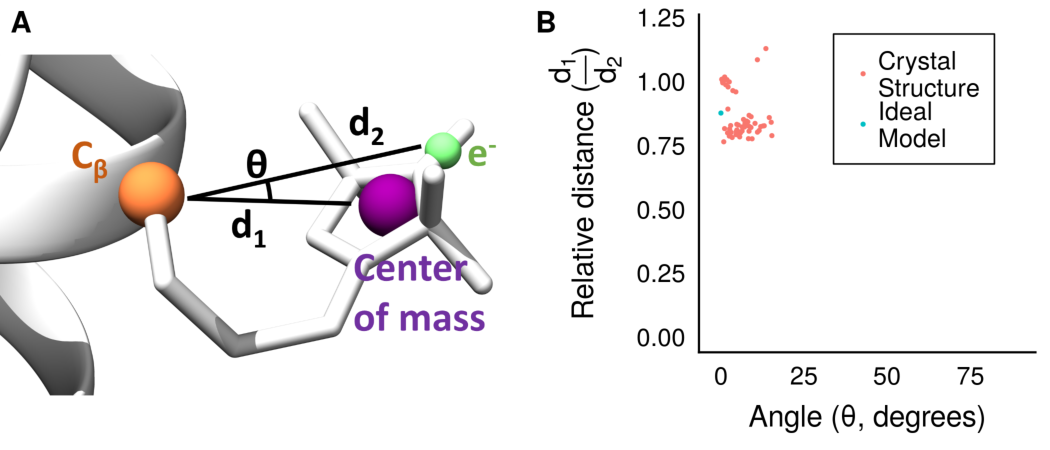
\includegraphics[width=6in]{Figures/rosettadeer_supp_sl.pdf}
 \caption[Nitroxide centers of mass fall along the $\mathrm{C_{\upbeta}}$-electron vector.]{Nitroxide centers of mass fall along the $\mathrm{C_{\upbeta}}$-electron vector. A) Depiction of spin label from PDB: 2Q9D showing the nitroxide center of mass (purple) and the nitroxide bond midpoint (green). B). Angle and relative distance of nitroxide center of mass along the $\mathrm{C_{\upbeta}}$-electron vector.}
\label{fig:rosettadeer_supp_sl}
\end{figure}

\begin{figure}[h]
\centering
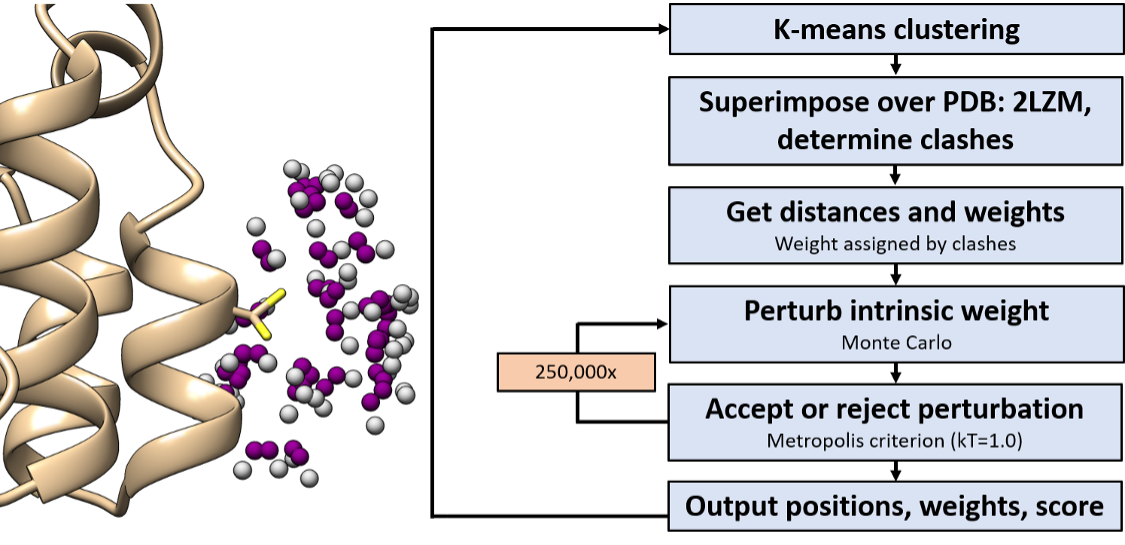
\includegraphics[width=6in]{Figures/rosettadeer_supp_scheme.pdf}
 \caption[Optimization of RosettaDEER measurement coordinates.]{Optimization of RosettaDEER measurement coordinates. Left: Each of the rotamers in Rosetta’s \gls{mtssl} rotamer library was converted into two coordinates: one representing the nitroxide ring center of mass (purple), which was used to evaluate clashes; and one representing the nitroxide bond midpoint (silver), from which distances were measured. Shown over PDB 2CUU residue 131. Right: Optimization scheme for reducing the number of measurement coordinates using experimental T4 Lysozyme distance data. One thousand replicates were performed for each of N clusters, with N ranging from 3 to 53 coordinates.}
\label{fig:rosettadeer_supp_scheme}
\end{figure}

\begin{figure}[h]
\centering
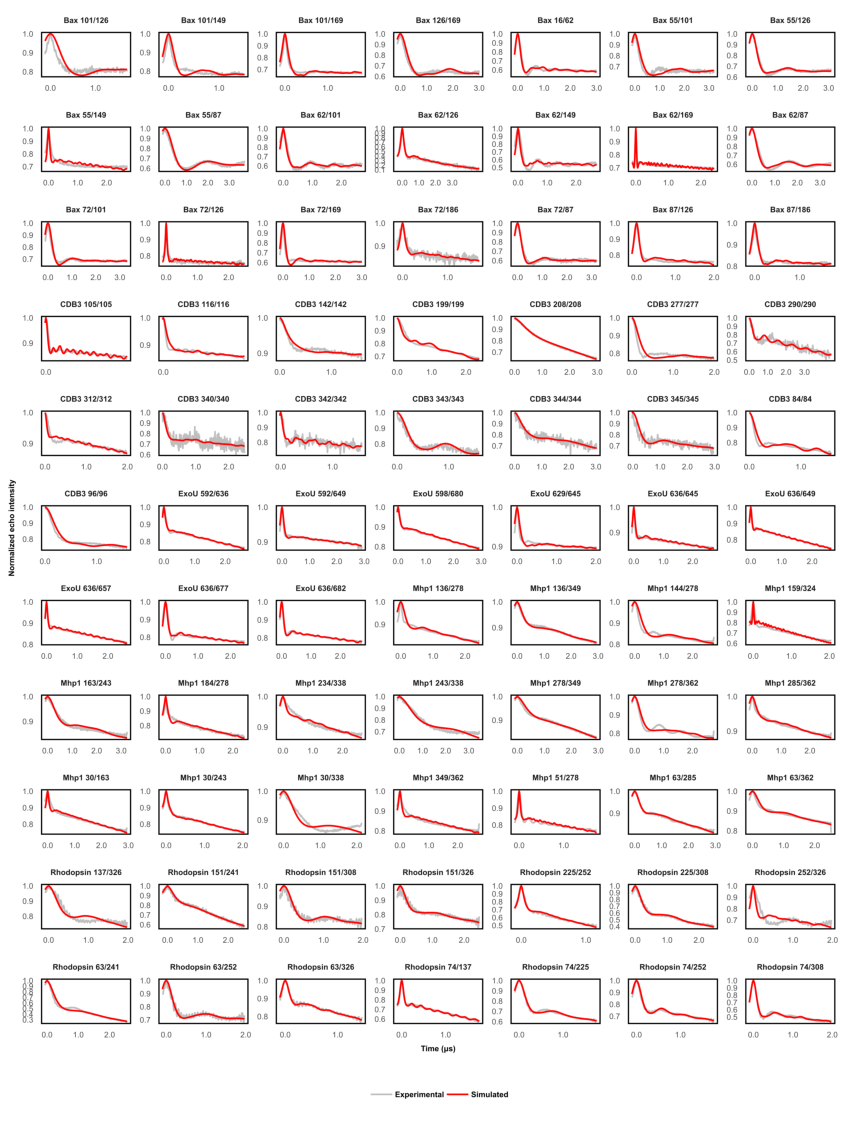
\includegraphics[width=5.5in]{Figures/rosettadeer_supp_alltraces.pdf}
 \caption[All simulated and experimental DEER decay data used in this study between experimentally resolved residues.]{All simulated and experimental DEER decay data used in this study between experimentally resolved residues. RosettaDEER could generally, but not always, simulate DEER traces from native-like models that are comparable to the experimental data.}
\label{fig:rosettadeer_supp_alltraces}
\end{figure}

\begin{figure}[h]
\centering
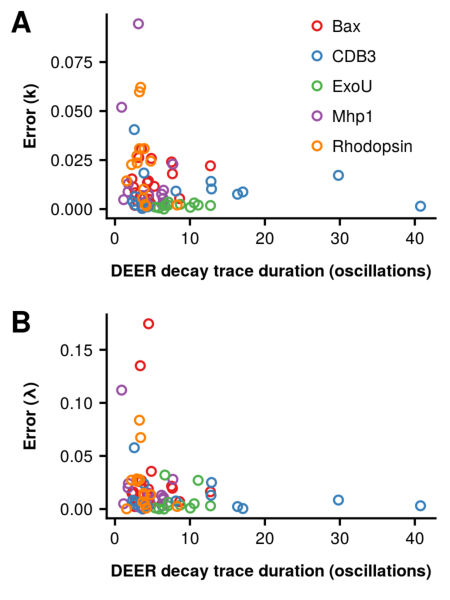
\includegraphics[width=3in]{Figures/rosettadeer_supp_oscillations.pdf}
 \caption[Deviation between experimental and simulated background decay ($k$) and modulation depths ($\lambda$).]{Deviation between experimental and simulated background decay ($k$) and modulation depths ($\lambda$).}
\label{fig:rosettadeer_supp_oscillations}
\end{figure}

\begin{figure}[h]
\centering
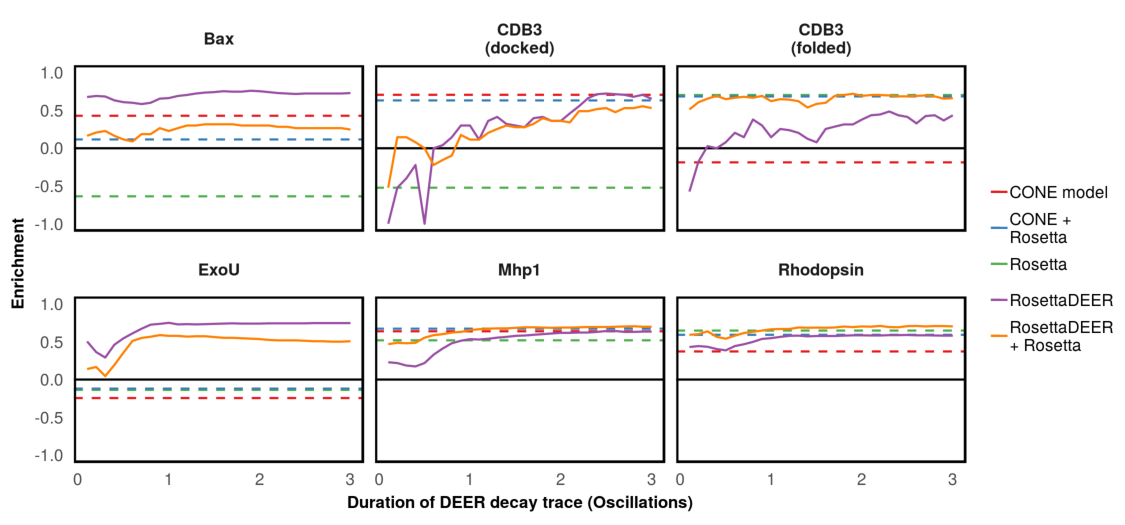
\includegraphics[width=5.5in]{Figures/rosettadeer_supp_oscillation_decoys.pdf}
 \caption[Enrichment of misfolded and misdocked decoys as a function of DEER decay trace duration.]{Enrichment of misfolded and misdocked decoys as a function of DEER decay trace duration. Enrichment was quantified as the logarithm of the percentage of native-like models (top 10\% by $\mathrm{RMSD_{100SSE}}$) that were also in the top 10\% by score. An enrichment of 1 indicates that the set of models constituting the top 10\% by RosettaDEER score was identical to the set of models constituting the top 10\% by Rosetta score.}
\label{fig:rosettadeer_supp_oscillation_decoys}
\end{figure}

\begin{figure}[h]
\centering
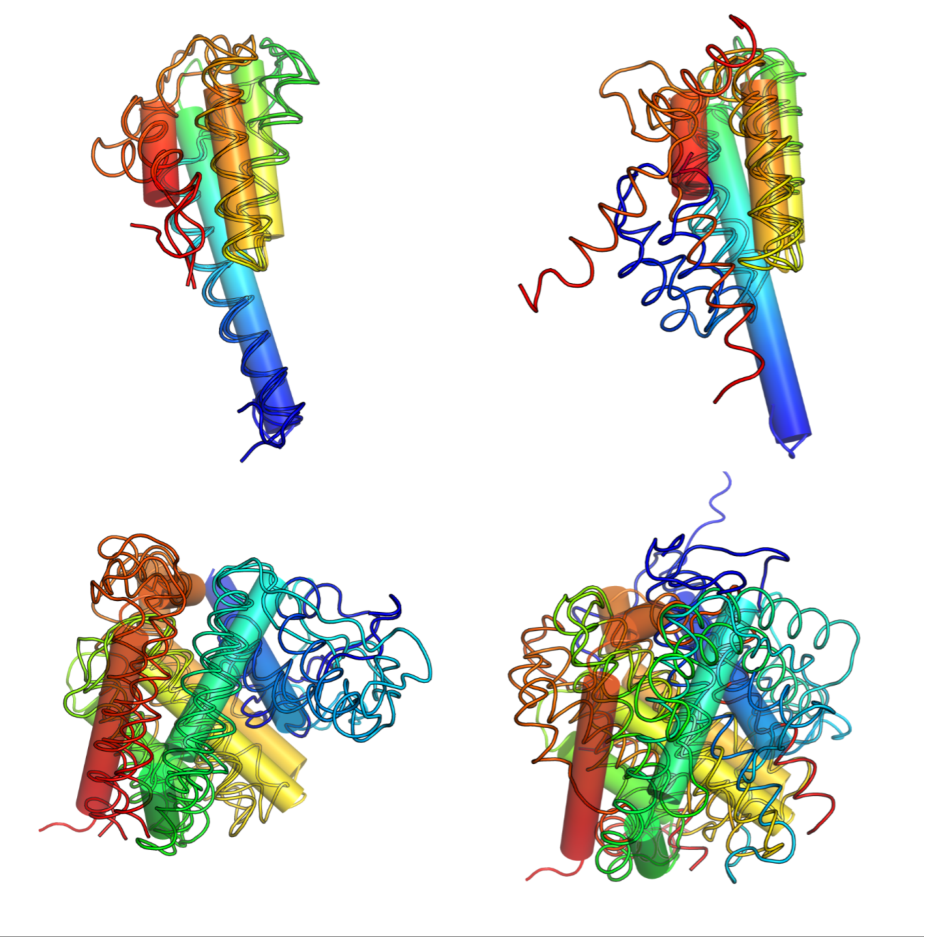
\includegraphics[width=5.5in]{Figures/rosettadeer_supp_top3.pdf}
 \caption[Effect of DEER restraints on structure prediction of Bax and ExoU. ]{Effect of DEER restraints on structure prediction of Bax and ExoU. Top 3 best-scoring models of ExoU (top) and Bax (bottom) folded either with (left) or without (right) experimental \gls{deer} restraints. The native models are shown as cylinders for comparison.}
\label{fig:rosettadeer_supp_top3}
\end{figure}

%\vspace{-7mm}
\bigskip

\clearpage % clear the prior chapter's page

\chapter{Supplement to "Methodology for rigorous modeling of protein conformational changes by Rosetta using DEER distance restraints"} \label{app:multilateration_supp}
%\vspace{-7mm}
%\bigskip

This Appendix contains supplementary information for Chapter \ref{ch:multilateration}.

%\vspace{-7mm}
%\bigskip

\begin{figure}[h]
\centering
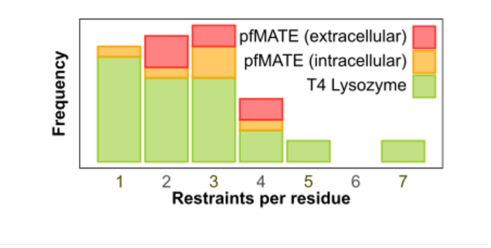
\includegraphics[width=2.5in]{Figures/multilateration_supp_n_restraints.pdf}
 \caption[Number of DEER restraints per spin-labeled residue across T4 Lysozyme and PfMATE.]{Number of DEER restraints per spin-labeled residue across T4 Lysozyme and PfMATE.}
\label{fig:multilateration_supp_n_restraints}
\end{figure}

\begin{figure}[h]
\centering
\includegraphics[width=6in]{Figures/multilateration_supp_alltraces.pdf}
\caption[All simulated and experimental DEER decay data used in this study between experimentally resolved residues.]{All simulated and experimental DEER decay data used in this study between experimentally resolved residues. All DEER traces determined by multilateration are shown in red. Experimental DEER traces are shown in black.}
\label{fig:multilateration_supp_alltraces}
\end{figure}

\begin{figure}[h]
\centering
\includegraphics[width=6in]{Figures/multilateration_supp_gladdvu.pdf}
\caption[Comparison of distributions obtained using GLADDvu and those using the RosettaDEER multilateration algorithm.]{Comparison of distributions obtained using GLADDvu and those using the RosettaDEER multilateration algorithm. All DEER distance distributions determined by multilateration are shown in black. DEER distributions calculated using GladdVU are shown in green, with the shaded regions indicating 95\% confidence intervals. Distance values shorter than \SI{15}{\angstrom} (indicated by the dashed line) were not used to simulate DEER traces.}
\label{fig:multilateration_supp_gladdvu}
\end{figure}

\begin{figure}[h]
\centering
\includegraphics[width=6in]{Figures/multilateration_supp_deeranalysis.pdf}
\caption[Comparison of distributions obtained using DeerAnalysis and those using the RosettaDEER multilateration algorithm.]{Comparison of distributions obtained using DeerAnalysis and those using the RosettaDEER multilateration algorithm. All DEER distance distributions determined by multilateration are shown in black. DEER distributions calculated using DeerAnalysis are shown in green, with the shaded regions obtained using the validation tool.}
\label{fig:multilateration_supp_deeranalysis}
\end{figure}

\begin{figure}[h]
\centering
\includegraphics[width=6in]{Figures/multilateration_supp_deernet.pdf}
\caption[Comparison of distributions obtained using DeerNet and those using the RosettaDEER multilateration algorithm.]{Comparison of distributions obtained using DeerNet and those using the RosettaDEER multilateration algorithm. All DEER distance distributions determined by multilateration are shown in black. DEER distributions calculated using DeerNet are shown in pink, with the shaded regions obtained using ensemble statistics.}
\label{fig:multilateration_supp_deernet}
\end{figure}

\begin{figure}[h]
\centering
\includegraphics[width=3.5in]{Figures/multilateration_supp_avgs_stdevs.pdf}
\caption[Comparison of average and standard deviation values obtained when fitting DEER data collected in pfMATE and T4 Lysozyme to values obtained using DeerAnalysis and DeerNet.]{Comparison of average and standard deviation values obtained when fitting DEER data collected in pfMATE and T4 Lysozyme to values obtained using DeerAnalysis and DeerNet. Long-distance fitting artifacts were removed from fits obtained using DeerAnalysis. These fits appeared to overstate the standard deviation values relative to GLADDvu, whereas those obtained using DeerNet appeared to be biased toward certain width values.}
\label{fig:multilateration_supp_avgs_stdev}
\end{figure}

\begin{figure}[h]
\centering
\includegraphics[width=6in]{Figures/multilateration_supp_conf_bands.pdf}
\caption[Confidence analysis among the five best-scoring rotamer ensembles generated using the RosettaDEER multilateration algorithm. ]{Confidence analysis among the five best-scoring rotamer ensembles generated using the RosettaDEER multilateration algorithm. Shaded regions depict 95\% confidence intervals, and line represents the mean distribution. Ensembles were selected using the \gls{aicc}.}
\label{fig:multilateration_supp_conf_bands}
\end{figure}

\begin{figure}[h]
\centering
\includegraphics[width=2.in]{Figures/multilateration_supp_validation.pdf}
\caption[Comparison of DEER distance distributions used to validate pseudo-rotamers obtained using the RosettaDEER multilateration algorithm.]{Comparison of DEER distance distributions used to validate pseudo-rotamers obtained using the RosettaDEER multilateration algorithm. Distributions obtained using GLADDvu and RosettaDEER are shown in green and grey, respectively. Confidence bands for RosettaDEER depict the five best sets of pseudo-rotamers.}
\label{fig:multilateration_supp_validation}
\end{figure}

\begin{figure}[h]
\centering
\includegraphics[width=2in]{Figures/multilateration_supp_scores.pdf}
\caption[Rosetta energy functions for membrane proteins cannot identify the inward-facing conformation of PfMATE.]{Rosetta energy functions for membrane proteins cannot identify the inward-facing conformation of PfMATE.  In all three cases, the lowest-energy models are fully occluded from both sides of the membrane. RMSD is measured from the inward-facing crystal structure (PDB: 6FHZ); the first 50 residues were omitted.}
\label{fig:multilateration_supp_scores}
\end{figure}
\clearpage % clear the prior chapter's page

\chapter{Supplement to "pH-dependent structural dynamics of the glutamate-GABA antiporter GadC"} \label{app:gadc_supp}
%\vspace{-7mm}
%\bigskip

This Appendix contains supplementary information for Chapter \ref{ch:gadc}.

\begin{figure}[h]
\centering
\includegraphics[width=3.5in]{Figures/gadc_supp_time_transport.png}
\caption[Time-dependent glutamate transport by wildtype and cysless GadC reconstituted into proteoliposomes filled with GABA.]{Time-dependent glutamate transport by wildtype and cysless GadC reconstituted into proteoliposomes filled with \SI{5}{mM} GABA.}
\label{fig:gadc_supp_time_transport}
\end{figure}

\begin{figure}[h]
\centering
\includegraphics[width=5.5in]{Figures/gadc_supp_transport45.pdf}
\caption[Glutamate transport activity by GadC cysteine mutants.]{Glutamate transport activity by GadC cysteine mutants. All experiments executed in triplicate and baseline-normalized. Wildtype transport rate is shown in black. Error bars show the standard error of the mean.}
\label{fig:gadc_supp_transport}
\end{figure}

\begin{figure}[h]
\centering
\includegraphics[width=5.5in]{Figures/gadc_supp_transport75.pdf}
\caption[pH-dependent inactivation of glutamate transport activity by GadC cysteine mutants.]{pH-dependent inactivation of glutamate transport activity by GadC cysteine mutants. Transport activity at pH 4.5 and 7.5 are shown in mauve and orange, respectively. All experiments executed in triplicate and baseline-normalized.}
\label{fig:gadc_supp_transport75}
\end{figure}

\begin{figure}[h]
\centering
\includegraphics[width=5in]{Figures/gadc_supp_substrates.pdf}
\caption[Representative EPR pairs do not show evidence of large-scale substrate-dependent conformational changes in GadC.]{Representative EPR pairs do not show evidence of large-scale substrate-dependent conformational changes in GadC. Top: DEER traces prior to and following background-correction. Middle: DEER distance distributions at pH 4.5 with \SI{1}{mM} GABA (orange) or glutamate (teal). Apo distributions shown in grey. Bottom: continuous-wave EPR lineshapes with or without substrates.}
\label{fig:gadc_supp_substrates}
\end{figure}

\begin{figure}[h]
\centering
\includegraphics[width=5in]{Figures/gadc_supp_tail.pdf}
\caption[pH-dependent DEER data and continuous-wave EPR spectra of GadC 143/480.]{pH-dependent DEER data and continuous-wave EPR spectra of GadC 143/480.}
\label{fig:gadc_supp_tail}
\end{figure}

\begin{figure}[h]
\centering
\includegraphics[width=6.5in]{Figures/gadc_supp_tail_rsq.png}
\caption[Correlation between short-distance DEER components in spin pair 143/480 during detachment of the tail.]{Correlation between short-distance DEER components in spin pair 143/480 during detachment of the tail.}
\label{fig:gadc_supp_tail_rsq}
\end{figure}

\begin{figure}[h]
\centering
\includegraphics[width=3.5in]{Figures/gadc_supp_bundle_hash_extra.pdf}
\caption[DEER data and CW profiles of double-cysteine mutants labeled on both the bundle and scaffold domains on the extracellular side.]{DEER data and CW profiles of double-cysteine mutants labeled on both the bundle and scaffold domains on the extracellular side.}
\label{fig:gadc_supp_bundle_hash_extra}
\end{figure}

\begin{figure}[h]
\centering
\includegraphics[width=3.5in]{Figures/gadc_supp_bundle_hash_intra.pdf}
\caption[DEER data and CW profiles of double-cysteine mutants labeled on both the bundle and scaffold domains on the intracellular side.]{DEER data and CW profiles of double-cysteine mutants labeled on both the bundle and scaffold domains on the intracellular side.}
\label{fig:gadc_supp_bundle_hash_intra}
\end{figure}


\begin{figure}[h]
\centering
\includegraphics[width=3.5in]{Figures/gadc_supp_el4.png}
\caption[DEER data and CW profiles of double-cysteine mutants labeled in EL4 and the scaffold domain on the extracellular side.]{DEER data and CW profiles of double-cysteine mutants labeled in EL4 and the scaffold domain on the extracellular side.}
\label{fig:gadc_supp_el4}
\end{figure}

\begin{figure}[h]
\centering
\includegraphics[width=3.5in]{Figures/gadc_supp_il1.pdf}
\caption[DEER data and CW profiles of double-cysteine mutants labeled in IL1 and the scaffold domain on the extracellular side.]{DEER data and CW profiles of double-cysteine mutants labeled in IL1 and the scaffold domain on the extracellular side.}
\label{fig:gadc_supp_il1}
\end{figure}

\begin{figure}[h]
\centering
\includegraphics[width=3.5in]{Figures/gadc_supp_bundle_only.pdf}
\caption[DEER data and CW profiles of double-cysteine mutants labeled in the bundle domain.]{DEER data and CW profiles of double-cysteine mutants labeled in the bundle domain.}
\label{fig:gadc_supp_bundle_only}
\end{figure}

\begin{figure}[h]
\centering
\includegraphics[width=6.5in]{Figures/gadc_supp_models.pdf}
\caption[Positions of the transmembrane helices among the five best low pH (pink) and high pH (gray) models relative to crystal structure (shown in red, green, blue, and yellow for bundle domain, hash domain, gating helices and EL4, respectively).]{Positions of the transmembrane helices among the five best low pH (pink) and high pH (gray) models relative to crystal structure (shown in red, green, blue, and yellow for bundle domain, hash domain, gating helices and EL4, respectively).}
\label{fig:gadc_supp_models}
\end{figure}

\begin{figure}[h]
\centering
\includegraphics[width=5.5in]{Figures/gadc_supp_rosettafold.pdf}
\caption[Experimental DEER distance distributions measured in GadC and compared to a model generated \emph{de novo} using RosettaFold.]{Experimental DEER distance distributions measured in GadC and compared to a model generated \emph{de novo} using RosettaFold.}
\label{fig:gadc_supp_rosettafold}
\end{figure}
\clearpage % clear the prior chapter's page

\chapter{Supplement to "Efficient sampling of loop conformations using conformational hashing and random coordinate descent"} \label{app:loophash_supp}
%\vspace{-7mm}
%\bigskip

This Appendix contains supplementary information for Appendix \ref{app:loophash}.


\begin{wraptable}{R}{0.5\textwidth}
\scriptsize
\renewcommand{\tabcolsep}{0.09cm}
\centering
\caption[Protein structures used in the benchmark of Hash/RCD.]{Protein structures used in the benchmark of Hash/RCD.}

\newcolumntype{Y}{>{\raggedright\arraybackslash}X}

\begin{center}
\begin{tabular}{l l r}
\toprule \\
\textbf{Protein } & \textbf{PDB ID} & \textbf{Length} \\
\midrule \\
\multicolumn{3}{l}{\textbf{Soluble proteins}} \\
Ribosomal protein S15 & 1A32 &	88\\
Acanthamoeba castellani profilin IB & 1ACF &	125\\
A-spectrin SH3 domain (D48G) & 1BK2 &	57\\
$\mathrm{\upbeta}$-Spectrin (CH domain)& 1BKR &	109\\
TRP1/HSC70 & 1ELW &	252\\
HSD (S46D) & 1OPD &	85\\
Streptococcal protein G & 1PGX &	83\\
Phage 434 repressor & 1R69 &	69\\
XcR50 & 1TTZ &	87\\
Ubiquitin & 1UBI &	76\\
Topoisomerase I & 1VCC &	77\\
Glia maturation $\mathrm{\upgamma}$-factor & 1VKK &	154\\
APE2540 & 1WDV &	304\\
Acetylcholinesterase & 2ACY &	98\\
CheY & 2CHF &	128\\
YeeU & 2H28 &	260\\
SLC9A3R2 & 2HE4 &	90\\
HigA & 2ICP &	94 \\
\\
\multicolumn{3}{l}{\textbf{Membrane proteins}} \\
Aquaporin & 1J4N &	271\\
Mitochondrial ADP/ATP carrier & 1OKC &	297\\
Glycogen phosphorylase B & 1PY6 &	498\\
V-type ATPase & 2BL2 &	1560\\
GlpG & 2IC8 &	182\\
DsbB & 2K73 &	183\\
KdpD & 2KSF &	107\\
Rhodopsin II & 2KSY &	247\\
GlpG & 2NR9 &	196\\
ApcT & 3GIA &	444\\
Riboflavin uptake protein & 3P5N &	378\\
\bottomrule \\
\end{tabular} 
\end{center}

\label{tab:loophash_benchmark}
\end{wraptable}
% \clearpage % clear the prior chapter's page

\chapter{Alternating access in LeuT-fold transporters}\label{ch:leutintro}
%\vspace{-7mm}
%\bigskip

\section{Introduction}
Secondary active transporters tap the potential energy stored in electrochemical gradients to allow cells to import and export nutrients and cytotoxic drugs as needed \citep*{Bosshart2019}. Despite a divergence in topologies and ligands \citep*{Drew2016, Shi2013}, these transporters are believed to operate via alternating access, a generic term referring to the exposure of the substrate-binding site to no more than one side of the membrane at a time \citep*{Jardetzky1966, Mitchell1957}. This mechanism allows transporters to couple conformational changes critical to substrate binding and/or release while minimizing the uncoupled flux or leaking of ions down their electrochemical gradients. Although this basic working model of transport has been devised over sixty years ago \citep*{Jardetzky1966}, characterizing the precise molecular mechanisms relating substrate binding to translocation in individual proteins of interest presents a formidable scientific challenge. High-resolution structures cannot identify the movements underpinning alternating access unless a protein is captured in multiple distinct conformations \citep*{Hofmann2019, Perez2012}. As such, solution-state measurements, carried out in the absence or presence of various substrates under conditions permitting conformational interconversion, directly report on the transporter's energy landscapes and allows high-resolution snapshots to be assigned to specific intermediate states observed in the functional cycle \citep*{Juette2014, Liapakis1999, Mchaourab2011, Oganesyan2018}. Unfortunately, but not unexpectedly, few proteins have been so exhaustively characterized.

\begin{figure}[h!]
\centering
\includegraphics[width=6.5in]{Figures/leutintro_arch.pdf}
 \caption[Architecture of the bacterial amino acid transporter LeuT.]{Architecture of the bacterial amino acid transporter LeuT. (A) The sodium-coupled amino acid transporter LeuT. (B) The ten-transmembrane helix core consists of a bundle domain (highlighted in red), a hash domain (green), and a pair of gating helices (blue). (C) Cartoon depiction of the conserved transport domain showing the pseudo-twofold symmetry of the ten-helix core. Substrate-binding site indicated by the red X. (D) Inverted repeats in helices 1-5 and 6-10.}
\label{fig:leutintro_arch}
\end{figure}

The bacterial \gls{nss} homolog LeuT found in the thermophilic archaea \emph{Aquifex aeolicus} presents a rare example of a transporter that has been studied to this extent (Figure \ref{fig:leutintro_arch}) \citep*{Yamashita2005}. LeuT couples the import of small aliphatic amino acids such as leucine and alanine to an inward sodium gradient and an outward proton gradient \citep*{Zhao2010}. Nearly two decades of persistent investigation has produced a library of atomic-resolution crystal structures capturing conformational intermediate states \citep*{Fan2021, Gotfryd2020, Krishnamurthy2012, Malinauskaite2016, Singh2008, Yamashita2005} linked by solution-state experimental data collected using various techniques \citep*{Adhikary2017, Billesbølle2015, Billesbølle2016, Claxton2010, Kazmier2014a, Merkle2018, Zhao2011}. Collectively, this body of knowledge describes in exquisite detail the molecular and energetic basis of ligand-dependent conformational changes driving sodium-coupled amino acid transport.

In this chapter, we explore the extent to which structural homologs of LeuT, many of which are found in humans and whose dysfunction contribute to a range of diseases, undergo similar ligand-dependent structural rearrangements \citep*{Loland2015}. These homologs include mammalian \gls{nss}s, such as \gls{sert} and \gls{dat} \citep*{Beuming2006, Coleman2016, Penmatsa2013}, as well as a multitude of more distant homologs that have been identified across nearly a dozen families (Tables \ref{tab:leutintro_proteins1} and \ref{tab:leutintro_proteins2}). As many proteins with the LeuT-fold have been the subject of extensive study over the course of many decades and have been the subject of numerous recent reviews \citep*{Bozzi2021, Cheng2019, Chew2021,  ErrastiMurugarren2021, Henriquez2021, Krammer2019, Patching2018, Rudnick2019, Singh2018, Ziegler2010}, this chapter focuses on comparing their conformational changes, structural dynamics, and energy landscapes. Necessarily, emphasis is placed on \gls{nss}s which are the most extensively studied family of transporters with this topology.

\begin{table}[h!]
\scriptsize
\renewcommand{\tabcolsep}{0.09cm}
\centering
\caption[Curated library of LeuT-fold protein structures.]{Curated library of LeuT-fold protein structures. Conformations are assigned to either \gls{ofop}, \gls{ofoc}, \gls{oo}, \gls{ifoc}, or \gls{ifop}. Structures are marked if they were mutated ($\dagger$) or bound to inhibitors ($\ddagger$) or antibodies ($\mathsection$). Redundant structures have been omitted.}

%\newcolumntype{Y}{>{\raggedright\arraybackslash}X}

% Structures are marked if they were mutated ($\dagger$) or bound to inhibitors ($\ddagger$) or antibodies ($\mathsection$).}

\begin{center}
\begin{tabular}{l l l l l r}
\toprule \\
\textbf{Protein \emph{(Organism)}} & \textbf{Conf.} & \textbf{PDB ID} & \textbf{Resolution} & \textbf{Substrates} & \textbf{Reference} \\
\midrule \\

\multicolumn{5}{l}{\textbf{Neurotransmitter-sodium symporter family}} \\
$\mathrm{b^{0}AT1}$ \emph{(Homo sapiens)} & \gls{ofoc} & 6M17 & 2.90 \AA & Apo & \citep*{Yan2020b} \\
DAT \emph{(Drosophila melanogaster)} & \gls{ofop} & $\mathrm{4XP1^\mathsection}$ & 2.89 \AA & $\mathrm{2Na^+/Cl^-/Dopamine}$ & \citep*{Penmatsa2015} \\
GlyT1 \emph{(Homo sapiens)} & \gls{ifop} & $\mathrm{6ZPL}^{\dagger \ddagger \mathsection}$ & 3.94 \AA & $ \mathrm{2Na^+/Cl^-/Benzoylisoindoline}$ & \citep*{Shahsavar2021} \\
LeuT \emph{(Aquifex aeolicus)} & \gls{ofop} & $\mathrm{3TT1^{\dagger \mathsection}}$ & 3.10 \AA & $\mathrm{2Na^+}$ & \citep*{Krishnamurthy2012} \\
& & $\mathrm{3F3A^{\ddagger}}$ & 2.00 \AA & $\mathrm{2Na^+/Tryptophan}$ & \citep*{Singh2008} \\
& & 7DIXb & 3.49 \AA & $\mathrm{Na^+/Leucine}$ & \citep*{Fan2021} \\
& \gls{ofoc} & 2A65 & 1.65 \AA & $\mathrm{2Na^+/Leucine}$ & \citep*{Yamashita2005} \\
& & 5JAE & 2.50 \AA & Apo & \citep*{Malinauskaite2016} \\
& \gls{ifoc} & $\mathrm{6XWM^\dagger}$ & 2.60 \AA & $\mathrm{2Na^+/Phenylalanine}$ & \cite*{Gotfryd2020} \\
& \gls{ifop} & $\mathrm{3TT3^{\dagger \mathsection}}$ & 3.22 \AA & Apo & \citep*{Krishnamurthy2012} \\
MhsT \emph{(Bacillus halodurans)} & \gls{ifoc} & 4US3 & 2.10 \AA & $\mathrm{2Na^+/Tryptophan}$ & \citep*{Malinauskaite2014} \\
SERT \emph{(Homo sapiens)} & OFOp & $\mathrm{5I6Z^{\dagger \mathsection}}$ & 4.53 \AA & Apo & \citep*{Coleman2016} \\
& & $\mathrm{5I6X^{\dagger \ddagger \mathsection}}$ & 3.14 \AA & Paroxetine & \citep*{Coleman2016} \\
& \gls{ifoc} & $\mathrm{6DZZ^{\ddagger \mathsection}}$ & 3.60 \AA & Ibogaine & \citep*{Coleman2019} \\
\\
\multicolumn{5}{l}{\textbf{Amino acid-polyamine-organocation transporter family}}
\\
AdiC \emph{(Escherichia coli)} & OFOp & 3OB6 & 3.00 \AA & Arginine & \citep*{Kowalczyk2011} \\
& & 5J4I & 2.21 \AA & Apo & \citep*{Ilgu2016} \\
& & 5J4N & 2.59 \AA & Agmatine & \citep*{Ilgu2016} \\
& \gls{ofoc} & $\mathrm{3L1L^{\dagger}}$ & 3.00 \AA & Arginine & \citep*{Fang2009} \\
AdiC \emph{(Salmonella typhimurium)} & \gls{ofop} & 3NCY & 3.20 \AA & Apo & \citep*{Fang2009} \\
ApcT \emph{(Methanococcus janaschii)} & \gls{ifoc} & 3GIA & 2.32 \AA & Apo & \citep*{Shaffer2009} \\
$\mathrm{b^{(0,+)}AT1}$ \emph{(Homo sapiens)} & \gls{ifop} & 6LI9 & 2.30 \AA & Arginine & \citep*{Yan2020a} \\ 
& & 6LID & 2.70 \AA & Apo & \citep*{Yan2020a} \\
BasC \emph{(Carnobacterium} sp. AT7\emph{)} & \gls{ifop} & $\mathrm{6F2W^{\mathsection}}$ & 3.40 \AA & 2-Aminoisobutyrate & \citep*{Errasti-Murugarren2019} \\
& & $\mathrm{6F2G^{\mathsection}}$ & 2.92 \AA & Apo & \citep*{Errasti-Murugarren2019} \\
GadC \emph{(Escherichia coli)} & \gls{ifop} & 4DJI & 3.19 \AA & Apo & \citep*{Ma2012} \\
GkApcT \emph{(Geobacillus kaustophilus)} & \gls{ifoc} & 5OQT & 2.86 \AA & Alanine & \citep*{Jungnickel2018} \\
& & 6F34 & 3.13 \AA & Arginine & \citep*{Jungnickel2018} \\
Lat1 \emph{(Homo sapiens)} & \gls{ofop} & $\mathrm{7DSQ^{\ddagger}}$ & 3.40 \AA & Diiodotyrosine & \citep*{Yan2021} \\
& \gls{ifop} & $\mathrm{6IRS^{\ddagger}}$ & 3.30 \AA & JPH203 & \citep*{Yan2019} \\
& & $\mathrm{6IRT^{\ddagger}}$ & 3.50 \AA & BCH & \citep*{Yan2019} \\
& & $\mathrm{6JMQ^{\mathsection}}$ & 3.31 \AA & Apo & \citep*{Lee2019} \\
Lat2 \emph{(Homo sapiens)} & \gls{ifop} & 7CMH & 3.40 \AA & Tryptophan & \citep*{Yan2020} \\
xCT \emph{(Homo sapiens)} & \gls{ifop} & $\mathrm{7CCS^{\dagger}}$ & 6.20 \AA & Apo & \citep*{Oda2020} \\
\\
\multicolumn{5}{l}{\textbf{Cation-chloride cotransporter family}} \\
NKCC1 \emph{(Homo sapiens)} & \gls{ifop} & 6PZT & 3.46 \AA & Apo & \citep*{Yang2020} \\
NKCC1 \emph{(Danio rerio)} & \gls{ifop} & 6NPL & 2.90 \AA & $\mathrm{K^+/2Cl^-}$ & \citep*{Chew2019} \\
KCC1 \emph{(Homo sapiens)} & \gls{ifop} & 6KKT & 2.90 \AA & $\mathrm{K^+/2Cl^-}$ & \citep*{Liu2019} \\
& & 6KKR & 2.90 \AA &  Apo & \citep*{Liu2019} \\
KCC2 \emph{(Homo sapiens)} & \gls{ifop} & 7D8Z & 3.40 \AA & Apo & \citep*{Xie2020} \\
KCC3 \emph{(Homo sapiens)} & \gls{ifop} & $\mathrm{6M22^{\ddagger}}$ & 2.70 \AA & DIOA & \citep*{Chi2021} \\
& & 7D90 & 3.60 \AA & Apo & \citep*{Xie2020} \\
KCC4 \emph{(Homo sapiens)} & \gls{ifop} & 7D99 & 2.90 \AA & Apo & \citep*{Xie2020} \\
KCC4 \emph{(Mus musculus)} & \gls{ifop} & 6UKN & 3.65 \AA & $\mathrm{K^+/Cl^-}$ & \citep*{Reid2020} \\
\bottomrule \\
\end{tabular} 
\end{center}
\label{tab:leutintro_proteins1}
\end{table}

\begin{table}[h!]
\scriptsize
\renewcommand{\tabcolsep}{0.15cm}
\centering
\caption[Curated library of LeuT-fold protein structures (continued).]{Curated library of LeuT-fold protein structures (continued).}

%\newcolumntype{Y}{>{\raggedright\arraybackslash}X}

% Structures are marked if they were mutated ($\dagger$) or bound to inhibitors ($\ddagger$) or antibodies ($\mathsection$).}

\begin{center}
\begin{tabular}{l l l l l r}
\toprule \\
\textbf{Protein \emph{(Organism)}} & \textbf{Conf.} & \textbf{PDB ID} & \textbf{Resolution} & \textbf{Substrates} & \textbf{Reference} \\
\midrule \\
\multicolumn{5}{l}{\textbf{Betaine/carnitine/choline transporter family}} \\
BetP \emph{(Corynebacterium glutamicum)} & \gls{ofop} & $\mathrm{4DOJb^{\dagger}}$ & 3.25 \AA &Apo & \citep*{Perez2012} \\
& \gls{ofoc} & $\mathrm{4DOJa^{\dagger}}$ & 3.25 \AA & Apo & \citep*{Perez2012} \\
& \gls{oo} & 4AINa & 3.10 \AA & Apo & \citep*{Perez2012} \\
& \gls{ifoc} & 2WIT & 3.35 \AA & $\mathrm{2Na^+/Betaine}$ & \citep*{Ressl2009} \\
& \gls{ifop} & 3P03 & 3.35 \AA & $\mathrm{2Na^+/Choline}$ & \citep*{Perez2011} \\
CaiT \emph{(Escherichia coli)} & \gls{ifop} & 2WSX & 3.50 \AA & $\mathrm{\upgamma}$-Butyrobetaine & \citep*{Schulze2010} \\
& & 3HFX & 3.15 \AA & Carnitine & \citep*{Tang2010} \\
CaiT \emph{(Proteus mirabilis)} & \gls{ifop} & 2WSW & 2.29 \AA & Apo & \citep*{Schulze2010} \\
\\
\multicolumn{5}{l}{\textbf{Natural resistance-associated macrophage protein family}} \\
ScaDMT \emph{(Staphylococcus capitis)} & \gls{ifop} & $\mathrm{5M94^{\dagger \mathsection}}$ & 3.10 \AA & Apo & \citep*{Ehrnstorfer2014} \\ 
& & $\mathrm{5M95^{\dagger \mathsection}}$ & 3.40 \AA & $\mathrm{Mn^{2+}}$ & \citep*{Ehrnstorfer2014} \\ 
EcoDMT \emph{(Eremococcus coleocola)} & \gls{ofop} & $\mathrm{5M8K}^{\dagger}$ & 3.60 \AA & Apo & \citep*{Ehrnstorfer2017} \\
& & $\mathrm{5M87}^{\dagger}$ & 3.30 \AA & $\mathrm{Mn^{2+}}$ & \citep*{Ehrnstorfer2017} \\
DraNramp \emph{(Deinococcus radiodurans)} & \gls{ofop} & $\mathrm{6D91^{\dagger}}$ & 2.36 \AA & Apo & \citep*{Bozzi2019} \\
& & $\mathrm{6BU5^{\dagger}}$ & 3.30 \AA & $\mathrm{Mn^{2+}}$ & \citep*{Bozzi2019} \\
& \gls{ifoc} & $\mathrm{6C3I^{\dagger}}$ & 2.40 \AA & Apo & \citep*{Bozzi2019} \\
& \gls{ifop} & $\mathrm{5KTE^{\dagger \mathsection}}$ & 3.94 \AA & Apo & \citep*{Bozzi2016} \\
& & $\mathrm{6D9W^{\dagger \mathsection}}$ & 3.94 \AA & Apo & \citep*{Bozzi2019} \\
\\
\multicolumn{5}{l}{\textbf{Sodium-solute symporter family}} \\
vSGLT \emph{(Vibrio parahaemolyticus)} & \gls{ifoc} & 3DH4 & 2.70 \AA & $\mathrm{2Na^+/Galactose}$ & \citep*{Faham2008} \\
& \gls{ifop} & $\mathrm{2XQ2^{\dagger}}$ & 2.70 \AA & Apo & \citep*{Watanabe2010} \\
SiaT \emph{(Proteus mirabilis)} & \gls{ofop} & 5NV9 & 1.95 \AA & $\mathrm{2Na^+/}$Neuraminic acid & \citep*{Wahlgren2018} \\
& & 5NVA & 2.26 \AA & Apo &  \citep*{Wahlgren2018} \\
\\
\multicolumn{5}{l}{\textbf{Potassium uptake permease family}} \\
KimA \emph{(Bacillus subtilis)} & \gls{ifop} & 6S3K & 3.70 \AA & $\mathrm{3K^+}$ & \citep*{Tascon2020} \\
\\
\multicolumn{5}{l}{\textbf{Amino acid-auxin permease family}} \\
DrSLC38A9 \emph{(Danio rerio)} & \gls{ifop} & $\mathrm{6C08^{\dagger \mathsection}}$ & 3.17 \AA & Arginine & \citep*{Lei2018} \\
& & $\mathrm{7KGV^{\dagger \mathsection}}$ & 3.40 \AA & Apo & \citep*{Lei2021} \\
\\
\multicolumn{5}{l}{\textbf{Nucleobase-cation symporter-1 family}} \\
Mhp1 \emph{(Microbacterium tumefaciens)} & \gls{ofop} & 2JLN & 2.85 \AA & Apo & \citep*{Weyand2008} \\
& \gls{ofoc} & 4D1B & 3.80 \AA & $\mathrm{Na^+/Benzylhydantoin}$ & \citep*{Simmons2014} \\
& \gls{ifop} & 2X79 & 3.80 \AA & Apo & \citep*{Shimamura2010} \\
\\
\multicolumn{5}{l}{\textbf{Alanine/glycine-cation symporter family}} \\
AgcS \emph{(Methanococcus maripaludis)} & \gls{oo} & $\mathrm{6CSE^{\mathsection}}$ & 3.24 \AA & $\mathrm{Na^+/Alanine}$ & \citep*{Ma2018} \\
& & $\mathrm{6CSF^{\mathsection}}$ & 3.30 \AA & $\mathrm{Na^+/}$D-Alanine & \citep*{Ma2018} \\
\bottomrule \\
\end{tabular} 
\end{center}
\label{tab:leutintro_proteins2}
\end{table}

\section{Functional and structural diversity within the fold}

\subsection{The ten transmembrane helix topology}

Proteins in the LeuT-fold belong to the \gls{apc} superfamily of transporters \citep*{Vastermark2014} and share a core transport structure consisting of ten \gls{tmh}s related by pseudo-twofold symmetry \citep*{Forrest2008, Kazmier2017}. These ten helices can be subdivided into three domains: the bundle domain (\gls{tmh} 1, 2, 6, and 7), the hash domain (\gls{tmh} 3, 4, 8, and 9), and gating helices (\gls{tmh} 5 and 10; this Chapter uses this canonical numbering scheme and ignores N-terminal transmembrane helices). Additional N- and/or C-terminal helices uninvolved in transport flank this ten-helix core and vary across individual transporter families comprising the LeuT fold. Characteristically, \gls{tmh} 1 and 6 contain conserved unwound regions, observed near the geometric center of the ten-helix core, and their involvement in ligand coordination is a hallmark of the fold \citep*{Screpanti2007}. Importantly, structural similarity is not accompanied by sequence similarity: few structural motifs are identifiable at the sequence level \citep*{Billesbølle2015, Malinauskaite2014, Stolzenberg2017}, which prevented these protein families from being co-categorized prior to the determination of their structures \citep*{Beuming2006}.

\begin{figure}[h!]
\centering
\includegraphics[width=6.5in]{Figures/leutintro_panel.pdf}
 \caption[Structural diversity within the LeuT fold.]{Structural diversity within the LeuT fold. The LeuT fold is adopted by proteins found in a range of transporter families. PDB IDs, starting from top left: 2A65, 4US4, 5I6X, 6PZL, 3DH4, 5NVA; 4DJI, 6IRS, 6LI9, 6M23, 6S3K; 2JLN, 6CSE, 2WIT, 6D91, 6C08.}
\label{fig:leutintro_panel}
\end{figure}

The LeuT fold is perhaps best defined by its evolutionary persistence across families of transporters with sequences that appear unrelated (Figure \ref{fig:leutintro_panel}) \citep*{Abramson2009}. In addition to \gls{nss} \citep*{Cheng2019}, the LeuT fold has been found to be adopted by members of the \gls{sss} \citep*{Henriquez2021}, \gls{ccc} \citep*{Chew2021}, \gls{apc} transporter \citep*{ErrastiMurugarren2021}, \gls{nramp} \citep*{Bozzi2021}, \gls{ncs} \citep*{Patching2018}, and \gls{aaap} families. The same topology also describes representatives of proteins families unique to prokaryotes, such as those in the \gls{bcct} \citep*{Ziegler2010}, \gls{agcs}, and \gls{kup} families. Additionally, several transporter families lacking representatives in the PDB are predicted to have this fold (Figure \ref{fig:leutintro_unknowns}) \citep*{Saier2016, Tunyasuvunakool2021, Vastermark2014}.

\begin{figure}[h!]
\centering
\includegraphics[width=5.5in]{Figures/leutintro_unknowns.pdf}
 \caption[Predicted structural models of proteins belonging to LeuT-fold families with no representatives in the PDB.]{Predicted structural models of proteins belonging to LeuT-fold families with no representatives in the PDB. Transporter families are defined by the Transporter Classification Database, and each model was generated using AlphaFold2.}
\label{fig:leutintro_unknowns}
\end{figure}

\subsection{Functional variation within the LeuT fold}

Retention of this ten-helix core is all the more remarkable considering the extent to which the functions, ligands, and sequences of these proteins differ. Although the majority of LeuT-fold proteins studied thus far cotransport their substrates and driving ions, others exchange them in opposite directions (symport and antiport, respectively \citep*{Forrest2009}). The centrally located substrate-binding site, shared by symporters and antiporters, accommodates ligands ranging in size and charge from halogen ions and divalent metals to sugars and aromatic amino acids. Its manipulation by mutagenesis has been shown to alter substrate specificity profiles in LeuT (\gls{nss}) \citep*{Piscitelli2011, Zomot2007}, GAT-1 (\gls{nss}) \citep*{Zomot2007}, and BetP (\gls{bcct}) \citep*{Perez2014}, highlighting the involvement of this region in identifying and trafficking ligands.

Beyond plasticity at this specific site, structural features decorating the core transporter further contribute to functional specialization. A remarkable example is SLC38A9, which both exports amino acids from the lysosome and activates the regulatory complex mTORC1 under nutrient-rich conditions \citep*{Rebsamen2015, Wang2015}. An N-terminal domain elegantly couples these two functions by binding to the cytoplasmic cavity \citep*{Lei2021} and, following displacement by the transported substrate arginine, releases and binds to GTPases involved in downstream signaling \citep*{Fromm2020}. In an interesting case of convergent evolution, the C-terminal domain of the pH-dependent \gls{glu}/\gls{gaba} exchanger GadC arrests transport by binding to the intracellular cavity at neutral pH in a nearly identical conformation \citep*{Ma2012}. Autoinhibition by disordered terminal domains has also been directly visualized in several potassium-chloride symporters \citep*{Chi2021, Xie2020}. In other proteins, such as eukaryotic \gls{nss}s, disordered termini instead regulate transport by interacting with a range of cytoplasmic proteins \citep*{Cooper2019, Karam2018}. In BetP, a cytoplasmic C-terminal helical domain regulates transport in response to osmotic stress \citep*{Gueler2016, Kraemer2009}. These domains often go unobserved in structural studies \citep*{Coleman2016, Liu2019, Penmatsa2013} due to truncation or intrinsic disorder, prompting speculation regarding their role in transport.

\newpage

\subsection{Quaternary structures adopted by LeuT-fold transporters}

Recent structures obtained by \gls{cryoem} have bolstered the diversity of quaternary structures known to be adopted by these proteins. Whereas X-ray crystallography demonstrated that LeuT-fold transporters can assemble as homodimers (AdiC, vSGLT) \citep*{Faham2008, Gao2009}, homotrimers (BetP, CaiT) \citep*{Ressl2009, Schulze2010}, or heterodimers (GkApcT) \citep*{Jungnickel2018}, due to technical limitations only compact binding interfaces were observed. By contrast, oligomers visualized by \gls{cryoem} reveal a multitude of weaker, more flexible, and in some cases asymmetric binding interfaces \citep*{Chew2019, Lee2019, Oda2020, Tascon2020, Yan2020a, Yan2020b, Yan2019, Yan2020}. For example, the eukaryotic \gls{apc} transporters Lat1, Lat2, and xCT each associate with 4f2hc (also called CD98hc) \citep*{Jeckelmann2020, Oda2020, Yan2019, Yan2020}, a protein with a large extracellular domain and a single transmembrane helix that is uninvolved in transport (Figure \ref{fig:leutintro_panel}). The homologous \gls{apc} transporter $\mathrm{b^{(0,+)}AT1}$ further assembles into a dimer of dimers with rBAT, each of which resemble the Lat/4f2hc complexes \citep*{Wu2020, Yan2020a}. This dimer-of-dimers arrangement was even observed in the \gls{nss} $\mathrm{b^{0}AT1}$, which associates with Angiotensin-converting enzyme 2 (the experimental structure of this tetramer was determined as part of a larger complex involving the SARS-CoV-2 spike protein) \citep*{Yan2020b}. Notably, the N-terminal transmembrane helices of rBAT and 4f2hc bind to the hash domains of $\mathrm{b^{(0,+)}AT1}$ and the Lats, respectively, at a similar position as the C-terminal transmembrane helix of ACE2 to $\mathrm{b^{0}AT1}$. Separately, the eukaryotic \gls{ccc}s \citep*{ Chew2019, Chi2020, Liu2019, Reid2020, Yang2020} and the bacterial potassium transporter KimA \citep*{Tascon2020} both fold as homodimers with large domain-swapped cytoplasmic regions. Divergence in both the sequences of these protein families and the structures of their cytoplasmic domains may highlight a recurrent quaternary assembly mechanism, the extent of which has not yet come to light.

Finally, in many cases, the oligomeric interfaces observed by \gls{cryoem} appear to be weaker and more flexible than suggested by the crystal structures. In both Lat1 and KCC1, for example, substantial interdomain movements have been reported when comparing their respective inward-facing apo and outward-facing inhibitor-bound states \citep*{Liu2019, Yan2021, Yan2019, Yan2020, Zhao2020}. Molecular dynamics simulations of the homodimer KimA suggested that contacts between the two transport domains are transient and fleeting, as these domains are tethered to one another only by their intertwined cytoplasmic domains \citep*{Tascon2020}; similar observations were experimentally made in \gls{ccc}s \citep*{Chi2021}. Such arrangements sharply contrast with the interfaces observed in vSGLT \citep*{Faham2008, Watanabe2010}, BetP \citep*{Ressl2009}, and other oligomers determined by crystallography, and hint at future discoveries regarding how these transporters interact as part of larger complexes.

\subsection{Recurring elements of substrate binding}\label{sec:ligands}

These unique structural features and arrangements surround a highly conserved ten-helix architecture shown in Figure \ref{fig:leutintro_arch}.C that, in several cases, have been shown to retain ligand-binding modes across distantly related proteins (Figure \ref{fig:leutintro_ligands}). A widely discussed example is the conserved sodium site, termed Na2, found in the majority of sodium-coupled symporters \citep*{Faham2008, Ressl2009, Wahlgren2018, Weyand2008, Yamashita2005}. In fact, the Na2 site's recurrence in this fold prompted Chew \emph{et al.} to assign its position to the sodium-binding site in the sodium/potassium/chloride symporter NKCC1, which was subsequently corroborated by molecular dynamics simulations and mutagenesis experiments that severely abrogated transport \citep*{Chew2019, Janos2021}. Among symporters that bind two sodium ions (\gls{nss}s, SiaT \citep*{Wahlgren2018}, BetP \citep*{Khafizov2012}), no such conservation is observed in the position of the other sodium ion. In proton-coupled symporters and amino acid exchangers, positively-charged residues occupy this position (lysine in ApcT, GkApcT, and BasC, and arginine in CaiT \citep*{Errasti-Murugarren2019, Gao2009, Jungnickel2018, Schulze2010, Tang2010}), highlighting the malleability of substrate coupling throughout the fold. A noteworthy exception is the sodium-coupled amino acid symporter AgcS, which coordinates its only sodium at a position equivalent to LeuT's Na1 site, leaving the Na2 site unoccupied \citep*{Ma2018}. This is despite its alanine binding site overlapping nearly perfectly with the substrate binding sites of unrelated amino acid transporters from the \gls{nss} and \gls{apc} families (Figure \ref{fig:leutintro_ligands}.C). To our knowledge, no cations besides sodium ions and protons have been observed in this site, and no comparable degree of structural conservation has observed at other ligand-binding sites, such as those involved in binding potassium (transported by \gls{sert}, as well as the \gls{kup} and \gls{ccc} families) or chloride (transported by \gls{nss}s and \gls{ccc}s).


\begin{figure}[h]
\centering
\includegraphics[width=6.5in]{Figures/leutintro_ligands_hoz.pdf}
 \caption[Examples of conserved ligand coordination.]{Examples of conserved ligand coordination. (A) Sodium ions (orange) and leucine (pink) in LeuT. (B) Conservation of the Na2 site. (C) Partial recurrence of amino acid binding modes. Substrates colored white are shared in all four panels.}
\label{fig:leutintro_ligands}
\end{figure}


\section{Alternating access inferred from crystal and cryo-EM structures}

At the molecular level, alternating access involves the opening and closing of gates providing passage to the substrate-binding site from either the intracellular or extracellular spaces \citep*{Jardetzky1966} For transporters with the LeuT-fold, this principally manifests as isomerization between \gls{of} and \gls{if} states using a "rocking bundle" mechanism that forbids substrate entry and exit from the cytoplasmic or periplasmic side of the membrane, respectively \citep*{Forrest2009}. Despite their co-classification, however, closer examination at structural changes in these proteins reveals a striking lack of consensus over the molecular details of alternating access. Conformational divergence as the rule, not the exception, became apparent nearly a decade ago with the publication of high-resolution structures of Mhp1 \citep*{Shimamura2010, Weyand2008}, BetP \citep*{Ressl2009}, and LeuT \citep*{Kazmier2017, Krishnamurthy2012, Yamashita2005}, and has since been reinforced by similar studies in SERT \citep*{Coleman2016, Coleman2019}, DraNramp \citep*{Bozzi2016, Bozzi2019}, and Lat1/4f2hc (Figure \ref{fig:leutintro_aa}) \citep*{Yan2021, Lee2019, Yan2021}. Additional structures of AdiC \citep*{Fang2009, Gao2009} and vSGLT \citep*{Faham2008, Watanabe2010} in both open and occluded conformations, though limited to \gls{of} and \gls{if} states, respectively, further expand the ways in which these transporters grant access to the substrate-binding site. Overall, comparison of pairs of structures reveals fundamental differences in which helices move and which stay fixed (Figure \ref{fig:leutintro_rmsf}).

\begin{figure}[h!]
\centering
\includegraphics[width=6.5in]{Figures/leutintro_aa.pdf}
 \caption[Variations in structural dynamics within the LeuT-fold.]{Variations in structural dynamics within the LeuT-fold. Conformational dynamics of LeuT-fold transporters show striking differences in how alternating access is carried out. Dynamic and static helices are depicted as ribbons and cylinders, respectively. Bottom left: No individual \gls{sss} has been characterized in both \gls{of} and \gls{if} conformations.}
\label{fig:leutintro_aa}
\end{figure}

\begin{figure}[h!]
\centering
\includegraphics[width=6.5in]{Figures/leutintro_rmsf.pdf}
 \caption[Residue-level movements during IF-to-OF isomerization in various LeuT-fold proteins.]{Residue-level movements during \gls{if}-to-\gls{of} isomerization in various LeuT-fold proteins. Unresolved residues omitted from the plot. All structures were aligned using TM-Align \citep*{Xu2010, Zhang2005}.}
\label{fig:leutintro_rmsf}
\end{figure}

\subsection{Movement of gating helix TMH5}\label{sec:leutintro_tm5}

Along with the intracellular loop preceding it, \gls{tmh}5 ranks among the most consistently mobile and dynamic regions in the transporters studied so far \citep*{Stolzenberg2017}.  In \gls{of} conformations, \gls{tmh}5 nestles against the bundle domain helices \gls{tmh}1a and \gls{tmh}6b, forming the highly ordered intracellular "thick gate". In the IF state, by contrast, opening of the intracellular vestibule is driven by rearrangements that vary across families and even individual proteins within families. The contribution of \gls{tmh}5 to alternating access has been most extensively studied in \gls{nss}s \citep*{Stolzenberg2017}. A $\mathrm{G_{X}NP}$ sequence, strictly conserved within the family and partially conserved throughout the fold, putatively mediates both bending and unfolding motions instrumental to the initiation of substrate release (Figure \ref{fig:leutintro_tm5tm10}). Mutagenesis of glycine or proline severely abrogates transport \citep*{Malinauskaite2014}, highlighting the importance of the dynamic processes facilitated by this motif. First observed in a substrate-bound \gls{if}-occluded conformation of MhsT \citep*{Malinauskaite2014}, partial unwinding of \gls{tmh}5 has been corroborated in several \gls{nss}s by \gls{hdxms} studies under conditions promoting the \gls{if} conformation of each protein \citep*{Adhikary2017, Merkle2018, Moeller2019, Nielsen2019}. However, although \gls{if}-open structures of LeuT and \gls{sert} show this helix protruding out from the rest of the transporter \citep*{Coleman2016, Gotfryd2020, Krishnamurthy2012}, orthogonal measurements in LeuT both suggest that under \gls{if}-promoting conditions it adopts conformations where the intracellular cavity is occluded, rather than open \citep*{Kazmier2014, Shi2008, Zhao2011, Zhao2010}. As is elaborated below in Section \ref{sec:leutintro_nss_dynamics} below, however, these results are qualified by the frequent use of leucine, which has a low transport rate and nanomolar binding affinity \citep*{Singh2008}. Subsequent solution-state experiments bound to different amino acids found that quenching of fluorescent probes attached to the intracellular half of \gls{tmh}5 inversely correlated with transport rate \citep*{Billesbølle2015}, suggesting that this \gls{if}-occluded conformation may be less stable, relative to \gls{if}-open, when transporting substrates with higher turnover rates such as alanine. Nevertheless, in conjunction with other findings discussed below in Section \ref{sec:leutintro_nss_dynamics}, this points to a mechanism in which \gls{tmh}5 preferentially adopts the partially unwound occluded conformation when bound to its substrate but transiently bends to release substrates.

It is notable that \gls{tmh}5 adopts a similar, but not identical, conformation in \gls{if}-open Mhp1, which shares this $\mathrm{G_{X}NP}$ sequence \citep*{Shimamura2010}. Despite this agreement, \gls{epr} measurements revealed a degree of disorder in \gls{tmh}5 altogether absent from similar measurements carried out on LeuT in the presence of leucine \citep*{Kazmier2014a}. Interestingly, ApcT also shares a LeuT-like bend despite lacking a proline in \gls{tmh}5 at the equivalent position \citep*{Shaffer2009}. Since its structure has only been determined in a single conformation, and since its homologs such as GadC and BasC maintain a straight conformation of this helix \citep*{Jungnickel2018, Ma2012}, the extent to which the aforementioned \gls{nss} movements occur in ApcT and its homologs is unclear \citep*{Shi2010}. Finally, although \gls{tmh}5 is also involved in opening the intracellular cavity in DraNramp \citep*{Bozzi2019}, which also lacks the conserved mid-helical proline, it undergoes a rigid-body up-and-out translation rather than bending and unfolding. Many other \gls{if} structures, such as those observed in vSGLT and GkApcT, lack a fully resolved stretch of residues corresponding to \gls{il} 2, located between \gls{tmh}s 4 and 5, indicating a high degree of heterogeneity in the crystal lattice or \gls{cryoem} grid \citep*{Jungnickel2018, Watanabe2010}. Ultimately, the conformational variation observed across the fold in this loop and helix, combined with solution-state data indicative of local disorder, suggests that the protruded conformation observed in some proteins, though perhaps physiologically relevant and likely fundamental to the transport cycle, may not represent a well-defined low-energy state.

\begin{figure}[h]
\centering
\includegraphics[width=6.5in]{Figures/leutintro_tm5tm10_hoz.pdf}
 \caption[Pivoting of TMH5 and TMH10 is observed in a subset of LeuT-fold transporters.]{Pivoting of \gls{tmh}5 and \gls{tmh}10 is observed in a subset of LeuT-fold transporters. Top left: LeuT with \gls{tmh}4/5 and TM9/10 highlighted. Bottom: Movements of \gls{tmh}5 observed in \gls{nss}s, ApcT, and DraNramp in the IF state. Conserved proline residues are highlighted in LeuT, MhsT and Mhp1. Top right: Movement of \gls{tmh}0 in Mhp1.}
\label{fig:leutintro_tm5tm10}
\end{figure}

\subsection{Movement in gating helix TMH10}

Movement in \gls{tmh}10, despite its pseudosymmetry to \gls{tmh}5, is less frequently observed (Figure \ref{fig:leutintro_tm5tm10}.B). In \gls{nss}s, for example, no evidence has been collected that show involvement in either ligand-dependent conformational dynamics, or partial unwinding \citep*{Kazmier2014a, Merkle2018, Moeller2019, Nielsen2019}. Mhp1 shows some partial symmetry of \gls{tmh}10 to \gls{tmh}5 in both sequence and structure, with comparable increases in conformational heterogeneity detected by \gls{epr} under \gls{of}-stabilizing experimental conditions (Figure \ref{fig:leutintro_tm5tm10}) \citep*{Kazmier2014, Shimamura2010, Weyand2008}. However, the movement inferred from crystal structures is less dramatic than that of \gls{tmh}5. In both BetP and DraNramp, differences between their \gls{of}-closed and open conformations in this region, though less drastic than in Mhp1, are nonetheless unmistakable; indeed, the corresponding proline in \gls{tmh}10 facilitating this bend is strictly conserved in the \gls{bcct} family and partially conserved among \gls{nramp}s \citep*{Bozzi2021, Schulze2010}. Although the \gls{apc} transporter AdiC both shares this specific residue and shows evidence of this structural movement, its structural similarity to the eukaryotic homolog Lat1, which instead has a cysteine at the equivalent position, indicates that placement of the proline halfway across \gls{tmh}10 may be coincidental \citep*{Fang2009, Yan2021}.

\subsection{Helical pivoting in the bundle domain}\label{sec:leutintro_bundle}

LeuT's twofold pseudosymmetry initially appeared to imply that a rigid-body rotation of the bundle domain relative to the rest of the structure mediates alternating access \citep*{Forrest2008}. This proposal, although elegant, failed to predict subsequent structural evidence in two key respects. First, the contribution of this domain to alternating access, although prominent in some proteins, is far from universal. Movement in ancillary helices and loop regions has been observed in every protein studied thus far. Second, the bundle domain virtually never moves as a rigid body. The exception, Mhp1, locks the bundle domain into place and instead pivots the hash domain and gating helices around this scaffold \citep*{Weyand2008} (see Section \ref{sec:leutintro_hash} below).

Movements in \gls{tmh}1a embody the variable intradomain dynamics observed in these helices. Its apparent dissociation from the rest of the intracellular vestibule, observed in X-ray and \gls{cryoem} structures of \gls{nss}s and \gls{nramp}s \citep*{Bozzi2019, Coleman2019, Ehrnstorfer2014, Krishnamurthy2012}, has been verified in solution (both families, it should be noted, lack N-terminal helices and oligomeric interfaces capable of restricting the dynamics of \gls{tmh}1a; see Figure \ref{fig:leutintro_rmsf}). Particular controversy surrounds the relevance of the signature 45° pivot observed in LeuT, which has been attributed to both the use of short-chain detergents commonly used in membrane protein crystallography \citep*{Moeller2020, Sohail2016}, as well as alanine mutagenesis of a conserved tyrosine residue essential for function \citep*{Krishnamurthy2012, Loland2002}. Molecular dynamics simulations of LeuT's \gls{if}-open crystal structure in a lipid bilayer later revealed the steep energetic cost of this movement into a more physiological membrane environment \citep*{Sohail2016}. Although this brought attention to the contribution of the membrane mimetic (along with a high-affinity antibody) in stabilizing such an extreme conformer, these findings, alongside experimental measurements obtained using both \gls{lret} \citep*{Sohail2016} and \gls{hdxms} \citep*{Adhikary2017} in lipid environments, nonetheless corroborated the more general hypothesis that \gls{tmh}1a becomes conformationally disordered in the \gls{if}-open state. Nevertheless, as these experiments were executed on similar tyrosine-to-alanine mutants, they do not address the extent to which this \gls{if}-open conformation is sampled by the wildtype protein in solution. For example, \gls{epr} measurements on equivalent tyrosine-to-alanine mutants recorded a comparable degree of disorder in \gls{tmh}1a; by contrast, no such dynamics were observed in variants without this mutation \citep*{Kazmier2014a, Merkle2018}. Follow-up experiments in \gls{sert} would paint a similar picture, with ibogaine, a ligand used to stabilize the \gls{if}-open structure during \gls{cryoem} studies, taking the role of this tyrosine-to-alanine mutation in LeuT \citep*{Coleman2019, Moeller2019}. Overall, the data suggest that the \gls{if}-open conformations of \gls{nss}s, and perhaps other proteins with similar conformational dynamics, transiently sample disordered \gls{tmh}1a states as part of their function, dovetailing with the conclusions on \gls{tmh}5 discussed above.

A similar pattern of increased disorder under \gls{if}-open-promoting conditions has also been observed in the intracellular side of \gls{tmh}7. In addition to the movements observed crystallographically, \gls{tmh}7 in LeuT appears to partially unfold under \gls{if}-favoring experimental conditions \citep*{Merkle2018}. For example, the eight N-terminal residues of this helix were not assigned to electron density in \gls{if}-open apo DraNramp \citep*{Bozzi2019}. The most pronounced motion of \gls{tmh}7 is likely found in Lat1, which swings over \SI{10}{\angstrom} to close its intracellular cavity \citep*{Yan2021}. As is discussed below, such a motion was suggested by, but not directly observed in, its bacterial homologs in the \gls{apc} family \citep*{Errasti-Murugarren2019, Ma2012}. Interestingly, no comparable movements are observed on the extracellular side of \gls{tmh}7. Unfortunately, the absence of data reporting the dynamics of transporters in the \gls{apc} family prevents any conclusions regarding increases in disorder in this helix from being established.

\gls{tmh}1b and \gls{tmh}6a, located on the extracellular sides of the protein, consistently undergo smaller scale but nonetheless significant dynamics essential to opening of the extracellular vestibule \citep*{Singh2008}. These helices appear to open the extracellular vestibule by moving in concert with the conserved helix \gls{el} 4, located between \gls{tmh}7 and \gls{tmh}8, in \gls{nss}s, \gls{apc} transporters, and \gls{nramp}s. While the observed movements of \gls{el}4 appear minor when compared to \gls{tmh}1a on the intracellular side, \gls{epr} spectroscopy data on LeuT indicate that crystal structures may understate the true extent to which these helices move \citep*{Kazmier2014}. Interestingly, on the intracellular side, no equivalent coupling between \gls{tmh}1a, \gls{tmh}6b, and \gls{il}1 has been detected to our knowledge. Indeed, unlike \gls{el}4, \gls{il}1 appears to be firmly stapled to the hash domain.

\subsection{The hash domain generally acts as a rigid body}\label{sec:leutintro_hash}

Relative to movements outlined above, independent helical movement within the hash domain are relatively rare. Mhp1 stands out in rocking this domain, alongside bending in \gls{tmh}5 and \gls{tmh}10, to fully mediate alternating access \citep*{Kazmier2014a, Shimamura2010, Weyand2008}. Similar movements were recorded in vSGLT using \gls{epr} \citep*{Paz2018}, although these coincided with additional movement distributed throughout the rest of the structure. As a point of contrast, other proteins limit their movements to bending of \gls{tmh}4 on the intracellular side and \gls{tmh}9 on the extracellular side to complement aforementioned movements of \gls{tmh}5 and \gls{tmh}10, respectively. The contribution of ancillary helices, which are frequently found adjacent to the hash domain, in explaining this phenomenon is unclear. In an interesting twist, a preprint publication describing the \gls{if}-to-\gls{of} transition in KCC1 proposes that alternating access is purely mediated by movement of \gls{tmh}3 and \gls{tmh}8, while \gls{tmh}4 and \gls{tmh}9 remain fixed \citep*{Liu2019, Zhao2020}.

\subsection{Conformational stabilization complicates the interpretation of these structures}

Importantly, many of these transporters, with Mhp1 and BetP being noteworthy exceptions, could only be coaxed into specific conformations using mutations, antibodies, or high-affinity transport inhibitors detrimental to function (see Tables \ref{tab:leutintro_proteins1} and \ref{tab:leutintro_proteins2}). In addition to the controversial use of a transport-abolishing tyrosine-to-alanine mutation in LeuT discussed above (Section \ref{sec:leutintro_bundle}) \citep*{Krishnamurthy2012}, stabilization of its \gls{if}-open state was also achieved by mutating a conserved tryptophan similarly found to be essential for function \citep*{Gotfryd2020}. Crystallographic capture of DraNramp in \gls{of} and \gls{if} conformations required glycine-to-arginine and glycine-to-tryptophan mutations near the unwound regions of \gls{tmh}1a and \gls{tmh}6a, respectively, that prevented isomerization by obstructing closure of the appropriate vestibule \citep*{Bozzi2016, Bozzi2019}. In human \gls{nramp}s, the equivalent missense mutation in \gls{tmh}1a is correlated with severely reduced iron uptake \emph{in vivo} \citep*{Barrios2012}, highlighting the extent to which transport function is impaired. Similarly, crystallization of \gls{if}-open vSGLT resulted from a lysine-to-alanine mutation that prevented ligand binding and showed no transport activity \citep*{Watanabe2010}. Capture of the OF-occluded conformation of AdiC, achieved using an aspartate-to-alanine mutation, may have played a role in stabilizing a ligand pose distinct from those observed in subsequent ligand-bound crystal structures of the wildtype protein \citep*{Gao2009}. Equivalent studies of the eukaryotic transporters \gls{sert} \citep*{Coleman2019}, Lat1 \citep*{Yan2021}, and KCC1 \citep*{Zhao2020} have employed a broad panel of potent inhibitors that preferentially bind to specific conformations. Whereas apo \gls{sert} readily crystallized in an \gls{of} conformation, capture of its \gls{if} conformation required the small molecule ibogaine \citep*{Coleman2019}. Similarly, both Lat1 and KCC1 were structurally characterized in \gls{if} conformations in the absence of ligands \citep*{Lee2019, Liu2019, Xie2020, Yan2020a} but could only be described in \gls{of} conformations using inhibitors \citep*{Yan2021, Zhao2020}. In each of these cases, the introduction of small molecules and/or inactivating mutations arrested transport by stabilizing conformers off-path with respect to the protein's functional cycle.

Nevertheless, assuming the physiological relevance of these structures, their comparison naturally prompts speculation regarding the evolutionary and/or functional basis for the variation in alternating access mechanisms. One proposal, made by the authors that determined the \gls{of} structure of KCC1, is the size of the ligand; only small-scale movements, limited to \gls{tmh}3 and \gls{tmh}8, are necessary for symport of the relatively small ions potassium and chloride \citep*{Zhao2020}. This hypothesis implies that larger substrates require larger movements and is supported by the observation that outward-locked DraNramp can transport protons, but not metals \citep*{Bozzi2019}. However, the small size of metals nonetheless raises questions about why DraNramp's \gls{of}-to-\gls{if} transition consists of such large-amplitude movements. Similarly, the relatively minor conformational changes observed in the transport cycle of BetP \citep*{Perez2012}, the substrates of which are comparable in size to amino acids, have been justified by function-specific adaptations. Ultimately, the insufficient data prevent any conclusions from being established in this respect.

\section{Connecting the dots: from structures to landscapes}

Proteins rarely navigate the conformational space accessible to them in the stepwise fashion suggested by depictions such as the one shown in Figure \ref{fig:leutintro_nss}. Mechanistic models of transport must necessarily, therefore, also map the conditions under which specific conformations occur. Secondary active transporters lack a molecular motor such as an ATPase and must therefore rely on the energy input provided by ions and ligands to undergo forward transport \citep*{Boudker2010}. The central question concerns how transporters harness this energy to undergo reconfigurations that ultimately result in productive transport. Unfortunately, the outstanding structural record of the LeuT-fold overrepresents static states amenable to structural characterization \citep*{Mullen2016, Tsai2010}. As a result, although the resulting structures enrich mechanistic models of transport, such as the glide-symmetry symport mechanisms proposed over two decades ago for \gls{nss}s \citep*{Rudnick2006} and \gls{ccc}s \citep*{Russell2000}, they are ill-equipped to directly test them. An example that will not be discussed further is the possible existence of an allosteric binding site in LeuT and other prokaryotic \gls{nss}s, which remains controversial despite over a decade of structural and experimental research \citep*{Fitzgerald2019, LeVine2019, Merkle2018, Piscitelli2010, Quick2009, Quick2012, Shi2010, Tavoulari2011}.

\subsection{Characterizing dynamics in the NSSs}\label{sec:leutintro_nss_dynamics}

The energy landscapes of \gls{nss}s are far better characterized than thoose of LeuT-fold proteins in other families and point to a striking degree of conservation. Measurements carried out in solution consistently demonstrate that sodium stabilizes OF conformations, ligands stabilize occluded conformations, and absence of either promotes flexible interconversion between \gls{if}-open and \gls{of}-open \citep*{Kazmier2014, Merkle2018, Terry2018, Zhang2018, Zhang2021}. These data provide additional context for these structures by reporting on how ligand-binding events bias the conformational ensemble, which can hint at the drivers of the transport cycle. At the same time, the data can reveal steps unanticipated by canonical symport and/or antiport mechanisms. For example, recent data suggesting that potassium stabilizes \gls{if}-open LeuT hint at a step in which intracellular potassium ions indirectly participate in the transport cycle by competing with sodium and accelerating their release from the central binding site \citep*{Billesbølle2016, Merkle2018} (facilitation of substrate release by allosterically bound ions has since been reported in KCC1 \citep*{Liu2019} and KCC2 \citep*{Zhang2021a} and suggested for KCC4 \citep*{Reid2020}).

These studies further highlight how homologs might diverge due to functional specialization. Despite their structural similarity, LeuT, \gls{sert} and \gls{dat} were observed to have slight variations in their conformational dynamics. Whereas LeuT adopts an \gls{if}-occluded conformation when bound to leucine \citep*{Kazmier2014a, Merkle2018}, \gls{sert} fluctuates between \gls{if}-occluded and \gls{if}-open \citep*{Moeller2019}. More intriguingly, the helical unwinding in \gls{il}2 and \gls{tmh}5 initially proposed by the \gls{if}-occluded structure of MhsT \citep*{Malinauskaite2014}, although plausible in LeuT and \gls{sert}, was altogether inconsistent with data collected in \gls{dat} suggesting a lack of cooperative movement in this region \citep*{Nielsen2019}. Comparable dynamics were instead observed in \gls{il}4, a nearby region that was previously found to be critical to \gls{if}-opening in other eukaryotic \gls{nss}s but static in LeuT \citep*{Hansra2004, Kazmier2014a} (lack of coverage in \gls{hdxms} studies of \gls{sert} prevented this region from being studied \citep*{Moeller2019}). However, the presence of lipids and cholesterol in \gls{dat} samples presents a confounding factor when attempting to directly compare these results to those collected in \gls{sert}, which was studied in detergent micelles. This suspicion is supported by previous studies that reported modulation of conformational dynamics in both eukaryotic \gls{nss}s and other secondary active transporters by detergent and lipids \citep*{Coleman2019, Damian2021, Jagessar2020, Martens2016, Moeller2019, Penmatsa2013, Zakrzewska2019}.

\begin{figure}[H]
\centering
\includegraphics[width=6.5in]{Figures/leutintro_nss.pdf}
 \caption[Conformational dynamics of neurotransmitter-sodium symporters inferred from crystal structures.]{Conformational dynamics of neurotransmitter-sodium symporters inferred from crystal structures. Top: LeuT couples the import of small aliphatic amino acids, such as leucine, to the inward and outward electrochemical gradients of sodium and protons, respectively. Bottom: Incomplete transport cycles of other \gls{nss}s. Inhibitor-bound states are highlighted in purple.}
\label{fig:leutintro_nss}
\end{figure}

Single-molecule visualization of conformational changes using \gls{fret} has added a layer of detail entirely missed by these ensemble-level measurements \citep*{Juette2014, Schuler2013}. A recent study employing this technique showed how LeuT appears to undergo uncoupled movement on the intracellular and extracellular sides of the membrane in the absence of substrate, including sampling a channel-like conformation simultaneously open to both sides \citep*{Terry2018}. Although canonical symport mechanisms of alternating access forbid this arrangement \citep*{Forrest2009}, LeuT appears to avoid uncoupled sodium flux by sealing the intracellular cavity in response to sodium binding. Additionally, this study corroborated previous experimental and computational studies on LeuT suggesting that substrate dissociation, and specifically ligand-dependent sodium dissociation from the Na2 site (see Section \ref{sec:ligands} above) \citep*{Billesbølle2015, Razavi2018}, is the rate-limiting step in transport. However, as mentioned above, this phenomenon may be unique to LeuT. A subsequent study on wildtype MhsT, in which soluble amino acid-binding proteins labeled with pairs of complementary fluorescent probes were cleverly introduced to the interior of MhsT-containing proteoliposomes, determined that the substrate-free \gls{if}-to-\gls{of} transition was instead rate-limiting \citep*{Fitzgerald2019}. Electrophysiology studies in human \gls{nss}s led to similar conclusions \citep*{Bhat2021}, suggesting that these discrepancies may be attributable to lower rates of transport and/or higher ligand-binding affinity observed in the thermophilic protein LeuT relative to transporters adapted to function at lower temperatures. 

\subsection{Differential dynamics in the SSS family}

The differences in conformational dynamics among \gls{nss}s, although not trivial, are dwarfed by those distinguishing them from \gls{sss}s such as the eukaryotic sodium/glucose symporter SGLT1, the prokaryotic sodium/galactose symporter vSGLT, and the prokaryotic sodium/proline symporter PutP. While not as well studied, these proteins traverse an energy landscape that is distinct from those of \gls{nss}s and indicative of the challenges inherent to the interpretation of solution-state dynamics data. \Gls{epr} measurements of vSGLT \citep*{Paz2018} and PutP \citep*{Raba2014} as well as fluorescent labeling and cysteine accessibility measurements in SGLT1 \citep*{Loo1998, Loo2006, SalaRabanal2012} suggest that ligand-dependent conformational dynamics were effectively inverted relative to \gls{nss}s, with apo and/or sodium-rich conditions favoring \gls{if} conformations and substrate binding stabilizing the \gls{of} conformation. As with \gls{nss}s discussed above, key differences between vSGLT and PutP were observed: no conformational response to sodium binding was detected in the former \citep*{Paz2018}, whereas sodium binding to the latter led to closing of \gls{el}4 and increased labeling of residues lining the intracellular vestibule \citep*{Jeschke2004a, Raba2014, Wegener2000}. Importantly, similar sodium-invariant conformational dynamics were independently reported in the unrelated bacterial transporter Mhp1 using both \gls{epr} and cysteine accessibility measurements \citep*{Kazmier2014, Calabrese2017, Weyand2011}, and sodium-driven stabilization of an \gls{if} state was also suggested by \gls{epr} data in BetP \citep*{Leone2019}.

Data from \gls{epr} studies on vSGLT prompted the conclusion that the sodium gradient is a critical driver of transport \citep*{Paz2018}. Consistent with this hypothesis, accessibility measurements and fluorescent labeling data collected in human SGLT1 in cells that actively maintain a sodium gradient showed a conformational landscape nearly identical to \gls{nss}s: unrestricted isomerization between \gls{of} and \gls{if} in the apo state \citep*{SalaRabanal2012} and stabilization of the \gls{of} conformation in the presence of sodium and absence of glucose \citep*{Loo1998, Meinild2002}. Critically, the \gls{of}-promoting effect of sodium diminished when the electrochemical gradient was decreased \citep*{Loo1998}. However, while these data support the hypothesis that the gradient may play a similar role in prokaryotic \gls{sss}s, a critical difference with unknown significance is SGLT1’s 2:1 sodium-to-glucose stoichiometry, which contrasts with the 1:1 stoichiometry of the prokaryotic model systems discussed above. 

\subsection{Energy landscapes in antiporters}\label{sec:leutintro_antiporters}

Missing from our knowledge of transporters with this fold is a detailed accounting of conformational dynamics data in antiporters. Despite their ubiquity in all domains of life and their extensive structural study by crystallography and \gls{cryoem} (Figure \ref{fig:leutintro_apc}), their energy landscapes remain virtually uncharacterized. Whereas canonical symport mechanisms, such as those broadly defining \gls{nss}s and \gls{sss}s, contain a substrate-free isomerization step, canonical antiport mechanisms facilitate substrate exchange by forbidding this conformational change \citep*{Forrest2009}. Instead, the second half of the antiport cycle involves the translocation of a second substrate in the opposite direction. In non-LeuT-fold antiporters, import of one molecule is proposed to power the energetically unfavorable export of another. For example, mechanisms of alternating access in unrelated transporters that expel toxic drugs frequently involve the cation-dependent stabilization of an \gls{if} conformation \citep*{Eisinger2017, Jagessar2020, Masureel2014}. The relevance of these findings to understanding LeuT-fold antiporters, however, is unclear, since many of them are not coupled to electrochemical ion gradients and instead function as substrate exchangers facilitating downhill translocation in opposite directions \citep*{Fang2009, Ma2012, Schulze2010, Tang2010}.

\begin{figure}[H]
\centering
\includegraphics[width=6.5in]{Figures/leutintro_apc.pdf}
 \caption[Structures and transport cycles of amino acid exchangers in the APC family.]{Structures and transport cycles of amino acid exchangers in the APC family. Top: The pH-activated precursor-product exchangers GadC and AdiC are co-transcribed with decarboxylases GadB and AdiA, respectively. Bottom: Canonical mechanisms of antiport forbid substrate-free conformational isomerization.}
\label{fig:leutintro_apc}
\end{figure}

A range of pH-dependent amino acid/polyamine antiporters in the \gls{apc} family, sometimes called "virtual proton pumps", import and export the precursors and products, respectively, of proton-consuming amino acid decarboxylases with which they are cotranscribed (Figure \ref{fig:leutintro_apc}) \citep*{Fang2009, Foster2004, Kanjee2013, Krammer2019, Ma2012}. Activation of these decarboxylases under extreme acidic conditions drains the intracellular concentration of the appropriate amino acids and raises that of the cognate polyamines, thus ensuring that both halves of the antiport cycle are energetically favorable. In fact, the two most well-characterized transporters, AdiC and GadC, are capable of forward and reverse transport of both substrates under equilibrium conditions \citep*{Ma2012, Ma2013, Tsai2013, Tsai2013a}. In contrast, they are inactive when their intracellular sides, but not extracellular sides, are exposed to protons, or in the presence of a negative-inside electric potential \citep*{Tsai2013, Tsai2013a}. One hypothesis proposed from \gls{md} simulations of AdiC posits that protonation of a conserved glutamate leads to the rate-limiting substrate dissociation from the central binding site \citep*{Zomot2011}, similar to the proposed role of potassium-induced substrate release on the intracellular side of LeuT (see section \ref{sec:leutintro_nss_dynamics}).

Homologs with broader substrate specificities such as BasC and Lat1 exchange amino acids in accordance with cellular needs while maintaining high intracellular amino acid concentrations \citep*{Errasti-Murugarren2019, Lee2019, Yan2019}. A critical adaptation in these proteins is their asymmetric binding affinity, with apparent Km values in the micromolar and millimolar range during out-to-in and in-to-out transport, respectively \citep*{Bartoccioni2019}. This is hypothesized to address the disparity between amino acid concentrations on the intracellular and extracellular side, which differ by several orders of magnitude. A secondary form of asymmetry in amino acid exchangers of the APC family is the selective import and export of charged substrates; $\mathrm{b^{(0,+)}AT1}$ selectively imports and exports cationic and neutrally charged amino acids, respectively, although neither the structures nor subsequent studies have shed light on the structural basis of this observation \citep*{Wu2020, Yan2020a}.

Unfortunately, the recent explosion of structures in the \gls{apc} transporter family has not been accompanied by studies into these proteins' energy landscapes. To our knowledge, the only study of dynamics in antiporters in the \gls{apc} family has been in the bacterial serine/threonine antiporter SteT \citep*{Reig2007} using single-molecule dynamic force spectroscopy, which reports on a protein's kinetic barriers \citep*{Bippes2009}. This study found that conformational flexibility in SteT increased under substrate-bound conditions relative to apo, consistent with the substrate-dependent conformational movement predicted by a canonical model of antiport. However, the data do not report on the protein's thermodynamics, which leaves critical questions about the protein's energy landscape unanswered.

\section{Comparison to homologous proteins}\label{sec:leutintro_homologs}

Overall, the outstanding evidence suggests that proteins in the LeuT-fold share few, if any, signature motifs of alternating access. To answer the question posed in the Introduction, differences in the structures and conformational dynamics of transporters both within and across families suggest that functional specialization has contributed to a degree of evolutionary divergence that prevents our rich knowledge of \gls{nss}s in general and LeuT in particular from being directly applied to less well-known families such as \gls{kup}s or \gls{aaap}s. However, the data also suggest that transporters in the same family are more similar to each other, both in structure and dynamics, than to proteins in other families. Thus, the question is one of evolutionary conservation at the family-level.

\subsection{Structural similarity within families of transporters}

From the perspective of structural similarity, the outstanding data suggest that homologs within a protein family show a degree of structural conservation not shared by other proteins with this fold. During their transport cycles, individual proteins sample conformations that differ by \SI{3}{\angstrom} $\mathrm{C_{\upalpha}}$ \gls{rmsd} \citep*{Ponzoni2018}. Structures of homologous proteins within and across families, meanwhile, differ by around \SI{3}{\angstrom} and \SI{5}{\angstrom} $\mathrm{C_{\upalpha}}$ \gls{rmsd}, respectively. This divergence has complicated the development of unified mechanistic models of transport for any protein or family because structural variation between different proteins could either reflect differences in sequence and function, or represent distinct steps in the transport cycle. Indeed, minor structural differences are even observed when comparing the structures of the same protein across different species, such as CaiT from \emph{Proteus mirabilis} and \emph{Escherichia coli} \citep*{Schulze2010}, AdiC from \emph{Salmonella typhimurium} and \emph{E. coli} \citep*{Fang2009}, NKCC1 from \emph{Homo sapiens} \citep*{Yang2020, Zhang2021a} and \emph{Danio rerio} \citep*{Chew2019}, and KCC4 from \emph{H. sapiens} \citep*{Xie2020} and \emph{Mus musculus} \citep*{Reid2020}.

An instructive example that was discussed in Section \ref{sec:leutintro_tm5} above is the varying position of \gls{tmh}5 in \gls{nss}s. The ligand-bound \gls{if}-occluded structure of MhsT \citep*{Malinauskaite2014, Stolzenberg2017} was interpreted as evidence that unwinding of \gls{tmh}5 is a feature preceding substrate release in all \gls{nss}s. In contrast, the conformation of \gls{tmh}5 in \gls{if}-occluded LeuT, which was corroborated by \gls{fret}, was bent and not unwound, which provided comparatively greater access to the intracellular vestibule \citep*{Gotfryd2020, Terry2018}, while the conformation of \gls{tmh}5 in \gls{if}-occluded \gls{sert} was described as "halfway" between that of LeuT and MhsT \citep*{Coleman2019}. It remains unclear if these structures represent distinct steps in a shared transport cycle, or if they reflect more fundamental differences between proteins resulting from functional specialization, evolutionary divergence, and/or environment-specific adaptations.

\subsection{Structural similarity between prokaryotic and eukaryotic transporters}

Nevertheless, the striking degree of structural correlation observed between distantly related proteins, particularly between bacterial and eukaryotic proteins, has been a recurring theme throughout studies of proteins with this fold. The first eukaryotic LeuT-fold transporter to be structural determined, the dopamine transporter \gls{dat} from \emph{Drosophila melanogaster} \citep*{Penmatsa2013}, bore a remarkable resemblance to LeuT, obtained from a thermophilic archaeum found in hot springs. Similarly, the structure of the \gls{apc} transporter GadC in an \gls{if} conformation \citep*{Ma2012} aligns well with those determined for the eukaryotic transporters Lat1/4f2hc \citep*{Lee2019, Yan2021, Yan2019}, Lat2/4f2hc \citep*{Jeckelmann2020, Yan2020}, and $\mathrm{b^{(0,+)}AT1}$ \citep*{Wu2020, Yan2020a}. This observation is all the more intriguing given that GadC's structure putatively represents an auto-inhibited state with no mechanistic equivalent in the transport cycles of these eukaryotic proteins \citep*{Ma2012, Ma2013}. Equally fascinating is the correspondence between the \gls{of}-open inactive conformations of Lat1 \citep*{Yan2021} and AdiC \citep*{Ilgu2016}. Unfortunately, comparison of eukaryotic and bacterial homologs is only possible in the \gls{nss} and \gls{apc} families, as the structurally determined proteins comprising every other family of transporters are either exclusively prokaryotic or exclusively eukaryotic.

Regarding the energy landscapes of these proteins, a dearth of dynamics data prevents straightforward comparisons from being made. It is nonetheless remarkable that the structural dynamics of vSGLT are more similar to those of Mhp1, which has identical 1:1 sodium-to-substrate stoichiometry despite being unrelated at the sequence level, than those of its homolog SGLT1, which instead mirror those of \gls{nss}s sharing its 2:1 sodium-to-substrate stoichiometry \citep*{Kazmier2014, Loo1998, Paz2018}. At the same time, given the variation in dynamics data observed among NSSs \citep*{Adhikary2017, Kazmier2014a, Merkle2018, Moeller2019}, small divergences in how \gls{sss}s respond to their substrates at the structural level appear to be expected.

\subsection{Implications of structural similarity and divergence on modeling}\label{sec:leutintro_modeling}

In 2008, vSGLT became the second protein, after LeuT itself, to be observed with the LeuT-fold \citep*{Faham2008}. Publication of its crystal structure in an \gls{if} conformation was complemented by an \gls{of} model generated from the structure of LeuT that attempted to predict which helices are involved in alternating access. Though this comparison is, with the benefit of hindsight, somewhat inappropriate, modeling of alternate conformers has since been a staple of structural studies that has guided experimental design \citep*{Geier2013, Gotfryd2020, Paz2018, Napolitano2017, Ylikangas2014}, generated starting points in simulations \citep*{Bisignano2018, Kelashvilli2015, Razavi2018}, and contextualized experimental findings \citep*{Kazmier2014a, Paz2018, Terry2018}. The previous discussion emphasized the risk of assuming that conformations observed in one protein are relevant to others, modeling has been particularly effective at extracting mechanistic insights into eukaryotic proteins from bacterial model systems \citep*{Bisignano2018, Forrest2008, Forrest2007, Geier2013, Wang2013, Zomot2007}.

Shortly after structure determination of LeuT in 2005, modeling studies led to the identification of the chloride-binding site of eukaryotic \gls{nss}s \citep*{Forrest2007, Zomot2007}. Chloride ions are not native ligands of LeuT, which instead exchanges two extracellular sodium ions and an amino acid with an intracellular proton \citep*{Zhao2010}. Nevertheless, by identifying a negatively-charge side chain near the sodium binding site exclusive to chloride-independent \gls{nss}s \citep*{Beuming2006}, this chloride-transporting phenotype could be introduced by mutating native glutamate and aspartate near the sodium-binding site of LeuT and the bacterial \gls{nss} Tyt1, respectively \citep*{Zomot2007}. Likewise, chloride-independent transport could be introduced in the \gls{gaba} transporter GAT1 by replacing the serine in the same position with a glutamate. In parallel, the chloride-binding site in \gls{sert} was identified by aligning its sequence to LeuT, and the resulting homology model predicted the chloride-binding position in \gls{sert} with astonishing detail \citep*{Forrest2008}.

Several drug discovery studies of Lat1 employed homology models, generated from \gls{if}-occluded ApcT \citep*{Shaffer2009} and \gls{of}-open AdiC \citep*{Gao2009}, to guide rational design of inhibitors and ligands \citep*{Geier2013, Napolitano2017, Singh2018, Ylikangas2014}. Although small details in the substrate-binding sites of these models were subsequently found to be inconsistent with the \gls{cryoem} structures \citep*{Lee2019, Yan2021, Yan2019}, they nonetheless facilitated the identification of multiple novel inhibitors. One of these inhibitors was later used to trap Lat1 in an OF-open conformation for \gls{cryoem} studies \citep*{Yan2021}, and the resulting structures verified the "carboxylate-up" orientation initially predicted by the homology model that had been observed in other transporters (Figure \ref{fig:leutintro_ligands}).

Finally, structural models have been invaluable in guiding restraint selection using sparse experimental data. A model of \gls{of} vSGLT, generated from the homologous SiaT \citep*{Wahlgren2018}, was used to determine which measurements to pursue using \gls{epr} \citep*{Paz2018}. Importantly, the \gls{of} model provided a context for the relatively sparse distance data and highlighted the flexibility of \gls{tmh}10 that was unanticipated. Additionally, prior to the structural determination of NKCC1 by \gls{cryoem}, cross-linking experiments were guided by computational models generated from AdiC; the conformation and register of \gls{tmh}s 10-12 predicted by this model was subsequently validated by \gls{cryoem} \citep*{Monette2014, Yang2020}.

\section{Scope of this dissertation}

The objectives of this dissertation are twofold.

The first objective focuses on studying the structural dynamics of the glutamate/GABA antiporter GadC. At low pH, GadC serves as a model system for other LeuT-fold antiporters, particularly those in the APC sub-family, while at high pH it putatively adopts an inactive conformation. As was discussed in section \ref{sec:leutintro_antiporters}, these transporters are far less well studied than homologous sodium-coupled symporters, and the extent to which their mechanisms of alternating access are conserved is unclear. Symporters such as LeuT, Mhp1, PutP, vSGLT, and SERT have been shown to undergo ligand-dependent changes in their conformational equilibria; whether GadC or homologous exchangers found in eukaryotes do the same is unknown. These questions are explored in Chapter \ref{ch:gadc} using \gls{epr} spectroscopy and computational modeling.

As will be discussed in Chapter \ref{ch:intro_deer}, the experimental data collected in GadC can report on changes in the distribution of distances between two spin labels but are local in nature and must be complemented with computational modeling to obtain global, fold-level structural insights. Thus, the second objective of this dissertation focuses on developing novel computational methods to model the structures of these proteins using these data. The Markov Chain Monte Carlo approach used throughout this text separates the modeling process into two steps, sampling and scoring. As is discussed in subsequent chapters, existing sampling and scoring methods do not effectively leverage the experimental data, leading to unacceptable losses in modeling precision and unnecessary increases in computation time. Therefore, this dissertation describes and discusses advancements in both halves of the modeling process. However, more attention is paid to the development of scoring approaches; the novel sampling approach is discussed further in Appendix \ref{app:confchangemover}. These sampling and scoring methods are combined to attempt to model conformational changes in three homologs of GadC using experimental \gls{epr} data.

One thread discussed in chapters \ref{ch:rosettadeer} and \ref{ch:multilateration} of this dissertation, unrelated to these two objectives, explores the extent to which the analysis of \gls{deer} data and its use for computational modeling can be integrated. In general, the time-domain data are first interpreted as distance distributions, which are in turn used as modeling restraints (see Chapter \ref{ch:intro_deer} for details). While several recent reports have begun to couple interpretation of the time domain data with structural modeling, the benefits of this approach have not been studied. Chapters \ref{ch:rosettadeer} and \ref{ch:multilateration} explore these approaches in greater detail for two specific tasks, predicting the folds of protein structures using sparse \gls{deer} and determining the positions of nitroxide rotamers, respectively. The goal of these two chapters is to determine the extent to which these two steps can be coupled. As is discussed in Chapter \ref{ch:rosettadeer}, this has the potential to advance the integration of computation and spectroscopy in a manner analogous to the prediction of protein structures using unassigned \gls{nmr} chemical shifts or raw SAXS scattering profiles. An overview of methods to analyze and simulate \gls{deer} data is provided in the following chapter. %As we discuss in section \ref{sec:multilateration_main_intro}, this has the potential to avoid propagating artifacts introduced during data analysis, which may negatively affect the quality of structural models.

%The work presented here focuses on studying and modeling the structure of GadC, a glutamate/GABA antiporter that is only active at low pH. Critical unanswered questions surround the effect of substrate on the transport cycles of antiporters in general as well as GadC's pH-dependent activation mechanism in particular. Both questions are answered using \gls{epr} studies comparable to those carried out in LeuT, Mhp1, and vSGLT mentioned earlier. Importantly, while these measurements are executed in the absence of a pH gradient, they are performed on protein reconstituted into lipid nanodiscs that more faithfully recapitulate the protein's native environment. Nevertheless, due to the low information content of \gls{epr}, modeling is necessary to translate these pairwise distance measurements into mechanistic insights. Thus, considerable attention is paid to the development of methods capable of accurately modeling structural states using these data, which are briefly reviewed in Chapter \ref{ch:intro_deer}. Chapter \ref{ch:rosettadeer} and Appendices \ref{app:scoring} and \ref{app:rosettadeer_supp} cover the methods developed for modeling proteins using \gls{deer} data. Chapter \ref{ch:multilateration} and Appendices \ref{app:confchangemover} and \ref{app:multilateration_supp} use these data to model conformational changes in several benchmark cases. Finally, Chapters \ref{ch:gadc} and \ref{app:gadc_supp} unite these methodological advancements and model the structure of GadC using experimental data collected at low and neutral pH. Chapter \ref{ch:conclusions} discusses the challenges that methods development must address to improve the precision of protein structural models, as well as how these integrative approaches might be applied in light of recent advancements in the field of structural biology.



\singlespacing

\end{document}
